\documentclass[12pt,fleqn]{report}
\usepackage{graphicx}
\usepackage{epstopdf}
\usepackage{amsmath}
\usepackage{natbib}
\usepackage{longtable}
\usepackage{appendix}
\usepackage{mathtools}
\usepackage{hyperref}
\usepackage{tikz}

% Workaround for longtable labels
\AtBeginDocument{%
\newlabel{tab:rentdata}{{}{}}%
\newlabel{tab:prepostdata}{{}{}}%
\newlabel{tab:bushdata}{{}{}}%
\newlabel{tab:outdata}{{}{}}%
}


\title{Notes on regression analysis for social research}
\author{E. C. Hedberg \\ hedbergec@gmail.com}
\date{}
\newcommand\intro[1]{
 \chapter*{#1}
 \markboth{\MakeUppercase{#1}}{}
 \addcontentsline{toc}{chapter}{#1}
}

\begin{document}
\maketitle
\tableofcontents
\listoftables
\listoffigures
\intro{About}
This document is a collection of my notes for an advanced regression course. It comes with no assurance of absolute accuracy. These notes are updated constantly and dated.

NOTE: These notes are based on the work of many statisticians and social scientists, and in no way reflect my own intellectual contributions.

I will eventually build a larger bibliography, but for right now these are just notes for a class. These notes are not designed to replace a proper text. ~\nocite{*}

I assume you have had a basic regression course and, of course, introduction to statistics. This is not about theory, and I go through the basics quickly.


\chapter{Univariate statistics}

\section{The mean, statistics, and parameters}
To calculate the mean, simply add up the numbers for each of the cases and divide by the total number of cases. For example, the mean of the numbers 1,2,3,4,5,6,7,8,9 is (1+2+3+4+5+6+7+8+9) / 9 = 41/9 = 4.556. Statisticians and mathematicians symbolize the addition of values in a set by using the summation symbol, $\Sigma$. The $\sum_{i=1}^{N}$ phrase represents the summation of each $i^{th}$ case, starting with the first one $i = 1$ and ending with the $N^{th}$ case. To calculate the mean, this sum is divided by $N$, or the total number of cases.

The formula of the mean is:
\begin{equation}\label{eq:mean}
\mu=\frac{\sum_{i=1}^{N}x_i}{N},
\end{equation}
which is estimated by the statistic:
\begin{equation}
\bar{x}=\frac{\sum_{i=1}^{N}x_i}{N}.
\end{equation}
In the previous paragraph, the term statistic is used. It is important to note that there are two concepts: parameters and statistics, which are often conflated by students. Frequentists generally think that the population at large can be described with parameters. For example, one parameter is the mean, or $\mu$. For example, a statistician might say that the population of objects (e.g., people) has some mean income. The statistician could then use a sample of objects to estimate this parameter. This estimate is the statistic.

For example, the estimate of the population mean, $\mu$, of some variable {\it x} is the mean statistic $\bar{x}$. If the variable was {\it w}, the statistic would be $\bar{w}$. The estimate of the population variance $\sigma^2$ is the statistic $s^2$. One way to think about this is with the mnemonic {\bf PPSS}: {\underline P}opulations have {\underline P}arameters, {\underline S}amples have {\underline S}tatistics.

Of course, these statistics are not going to be absolutely correct, and will vary from one sample to the next. Thus, one of the things that researchers fret most about is how well a certain statistic estimates a parameter. This is the sampling variation of that statistic, or the variance of the estimate. The square root of the variance of a statistic is the standard error. More on that later.
\section{Deviance}
The next important idea is that of deviance. This is central to most of what statistics is about since statisticians often wonder how one population differs from another that has experienced some effect or treatment. The most basic deviation is the difference between a case's value of {\it x} and the mean of {\it x}, $\bar{x}$. Deviance can be symbolized as:
\begin{equation}
  e_i=x_i-\bar{x}.
\end{equation}
Even this basic idea has substantive interest. It is often important to know how some case differs from what is typical. Here, the mean is considered typical, and it is valuable to know whether a case is typical, above typical, or below typical. Negative deviance values are below the mean, positive deviance values are above the mean, and 0 deviance is exactly the mean.
\section{The sum of squares}
It is often important to understand how much deviance there is in our sample. One method might be to add up each deviance score, but because of properties of the mean this will wind up at 0 which makes this a rather useless method. As luck would have it, there is a simple solution to this problem.

By squaring each deviance, the negative values of deviance are effectively made positive (since the square of any negative number is positive) and then by adding up each squared deviance term, a measurement of total deviance is obtained. We call this total deviance the sum of squares, or $SS$:
\begin{equation}
  SS=\sum_{i=1}^{N}e_i^2={\sum_{i=1}^{N}(x_i-\bar{x})^2}.
\end{equation}
One interesting way to view $SS$ is to consider it a measure of how much information is available in a variable. The larger the $SS$, the more information that is contained in the variable that can be modeled and correlated with other variables. If the $SS$ is small, then little will be correlated with it.
\section{The variance}
The next quantity is the variance. This is simply the average of $SS$. In the population, this is
\begin{equation}
  \sigma_x^2=\frac{{\sum_{i=1}^{N}(x_i-\bar{x})^2}}{N}.
\end{equation}
The estimate of the population variance is the sum of squared deviations divided by N-1:
\begin{equation}
  s_x^2=\frac{{\sum_{i=1}^{N}(x_i-\bar{x})^2}}{N-1}.
\end{equation}
We divide by N-1 instead of N because we lose a degree of freedom since this statistic employs another statistic (the mean). This is also a correction to remove bias, since this estimate of the population variance without this correction is slightly smaller than the expected parameter.
\section{The standard deviation}
A problem with the variance is that it in units of squared deviations. To get back to simple deviations, we take the square root of the variance to get the standard deviation. In the population this is
\begin{equation}
  \sigma_x=\sqrt{\frac{{\sum_{i=1}^{N}(x_i-\bar{x})^2}}{N}},
\end{equation}
and the statistic is
\begin{equation}
  s_x=\sqrt{\frac{{\sum_{i=1}^{N}(x_i-\bar{x})^2}}{N-1}}.
\end{equation}

\section*{For more information}
For foundational understanding of univariate statistics, see \citep{rice2007mathematical}, \citep{agresti}, and \citep{skk}.



\chapter{A little probability theory}
\label{sec:prob}

At the end of the day, all analyses are attempting to make some statement(s) with two parts:
\begin{itemize}
\item{Some assertion (or set of assertions)}
\item{The probability that this assertion is (or these assertions are) false}
\end{itemize}
Most of these notes focus on the methods to make such statements using a regression model of some sort. These regression models produce some {\it statistic} of interest, whether it is a coefficient, predicted value, or measure of model fit. Generally, all statistics have an associated {\it variance}, or measure of uncertainty that can generally be used to produce some estimated probability of observing the data on hand if we assume some (null) worldview.  Thus, we should never lose sight of keeping track of the probabilities associated with our assertions. The probability associated with an assertion depends on several factors:
\begin{itemize}
\item{The statistic being estimated, for example}
\subitem{a coefficient from a OLS regression}
\subitem{a coefficient from a GLS regression}
\subitem{a coefficient from a GLM regression}
\subitem{a coefficient from a Mixed regression model}
\item{The degrees of freedom associated with the statistic, if applicable}
\item{The distribution of the statistic, for example}
\subitem{z}
\subitem{t}
\subitem{F}
\subitem{$\chi^2$}
\item{How the data were collected, for example}
\subitem{Census or administrative data}
\subitem{Simple random sample}
\subitem{Stratified random sample}
\subitem{Cluster randomized sample}
\subitem{Stratified cluster randomized sample}
\end{itemize}

Therefore, it is important to remind ourselves of the basics of probability, random variables, and samples. This will not be a very in-depth discussion of these concepts, but should put you on notice to spend some time to better understand them as you start your research career.

The study of probability as a formal science started in $17^{th}$ century France when a gambler started talking to his mathematician buddies, namely, Pascal (yup, that Pascal). We generally care about probability not because the events we study are random, but that the observations we have in our data set, our {\it sample}, generally arrived there through some random process.

Here are some basic concepts, quickly.

The universe of possible events is considered the {\bf sample space}, which we can sometimes call $\Omega$. An element of the sample space is sometimes called $\omega$. For example, if we roll a dice, we have 6 possible sides than can land upright:
\[
\Omega = \left\{1,2,3,4,5,6\right\}
\]
From a sample space, we are generally concerned with a particular event occurring, for example, we can say that the event $A$ occurs when we roll a dice and a number greater than or equal to 5 shows up
\[
A = \left\{5,6\right\}
\]
or we can say that the even $B$ occurs when we roll a dice and a number less than or equal to 2 shows up
\[
B = \left\{1,2\right\}
\]
We can also say that the event $C$ is the union of $A$ and $B$ when either $A$ or $B$ occur
\[
C = A \cup B
\]
or
\[
C = \left\{1,2,5,6\right\}
\]
Suppose we had another even $D$, that is the number on the dice was even
\[
D = \left\{2,4,6\right\}
\]
We could say that the intersection of events $C$ and $D$ is event $E$
\[
E = C \cap D
\]
or
\[
E = \left\{2,6\right\}
\]
Of course, we could always get an empty set, that is a set with nothing in it. For example if we have event $F$, that the number of the dice is odd, then
\[
E \cap F = \emptyset
\]
in which case we can say that $E$ and $F$ are disjoint.

Here are some important laws
\begin{itemize}
\item{Communicative law}
\begin{equation}
A \cup B = B \cup A
\end{equation}
\begin{equation}
A \cap B = B \cap A
\end{equation}
\item{Associative law}
\begin{equation}
\left(A\cup B\right)\cup C = A \cup \left(B \cup C\right)
\end{equation}
\begin{equation}
\left(A\cap B\right)\cap C = A \cap \left(B \cap C\right)
\end{equation}
\item{Distributive law}
\begin{equation}
\left(A \cup B\right)\cap C = \left(A \cap C\right)\cup\left(B \cap C\right)
\end{equation}
\begin{equation}
\left(A \cap B\right)\cup C = \left(A \cup C\right)\cap\left(B \cup C\right)
\end{equation}
\end{itemize}

Next, we have the concept of a {\bf probability measure} on $\Omega$. A probability measure is a function $P$ that maps subsets of $\Omega$ to a real number. The rules (or axioms) are
\begin{itemize}
\item{The probability of the whole sample space is 1}
\begin{equation}
P\left(\Omega\right) = 1
\end{equation}
\item{If A a subset of the sample space, then the probability of greater than or equal to 0}
\begin{equation}
\mbox{if } A \subset \Omega \mbox{, then } P\left(A\right) \ge 0
\end{equation}
and the big one that makes a lot of things work:
\item{If $A$ and $B$ are disjoint, then the probability of either happening is the sub of the probabilities of each}
\begin{equation}
P\left(A \cup B\right) = P\left(A\right) + P\left(B\right)
\end{equation}
which generalizes to (if all $S$ sets $1\ldots N$ are disjoint)
\begin{equation}
P\left(\bigcup_{i=1}^N S_i\right)= \sum_{i=1}^N P\left(S_i\right)
\end{equation}
\end{itemize}

These axioms lead to several useful observations. First, the probability of a complement of a set $A$, $A^c$, is $1-P\left(A\right)$. Second, the probability of a empty set is 0, or $P\left(\emptyset\right) = 0$. Third, if $A \subset B$, then $P\left(A\right) \le P\left(B\right)$. Finally, $P\left(A \cup B\right) = P\left(A\right) + P\left(B\right) - P\left(A\cap B\right)$.

Other important observations and laws include the definition of conditional probabilities
\begin{equation}
P\left(A\mid B\right) = \frac{P\left(A\cap B\right)}{P\left(B\right)}
\end{equation}
assuming, of course, that $P\left(B\right) \neq 0$. This can work backwards,
\begin{equation}
P\left(A\cap B\right) = P\left(A\mid B\right)P\left(B\right)
\end{equation}
This makes life easier down the road when you consider the situation in which $B_1\ldots B_n$ are a set of mutually disjoint events with non-zero probabilities. In that case, you can get the total probability of another event $A$ with
\begin{equation}
P\left(A\right) = \sum_{i=1}^n P\left(A \mid B_i \right)P\left(B_i\right)
\end{equation}
Which leads to Bayes' rule. If we have the same circumstances, then we can actually find the probability of an event $B_j$ in the other way
\begin{equation}\label{eq:bayes}
P\left(B_j \mid A\right) = \frac{P\left(A\mid B_j\right)P\left(B_j\right)}{\sum_{i=1}^n P\left(A \mid B_i \right)P\left(B_i\right)}
\end{equation}

The frequentist approach produces probabilities of statistics on the basis of a hypothetical set of repeated samples or experiments. Bayesians, on the other hand, assert that the probability of a statistic should be based on the researchers quantification of the probability (usually based on computer simulations). Neither is without merit or warts. We take the frequentist approach here because it is more common, but not because it is necessarily "better."

This is all well and good, but how to you compute probabilities? Basically, if you have a sample space $\Omega$ with elements $\left\{\omega_1 \ldots \omega_n\right\}$, each element has a certain probability $P\left(\omega_i\right) = p_i$. If we want the probability of $A$, we add all the probabilities in the set $A$. For example, dice again, the probability of an even number roll when all sides are equally possible are
\[
\Omega = \left\{1,2,3,4,5,6\right\}
\]
where
\[
p_1 = \frac{1}{6}\ldots p_6= \frac{1}{6}
\]
so
\[
P\left(even\right) = p_2+p_4+p_6 = \frac{1}{6}+\frac{1}{6}+\frac{1}{6} = \frac{3}{6} = \frac{1}{2} = 0.5
\]
In general, if the sample space has $N$ elements, and if $A$ can occur in any $n$ mutually exclusive ways, then $P\left(A\right) = \frac{n}{N}$.

In order to talk samples, we now need to discuss permutations. A permutation is an ordered arrangement of elements--in other words, order matters in permutations. It is important to note whether our permutation occurs with or without replacement.

If we have a sample space of $N$ elements and a sample size of $n$, there are a possible $N^n$ number of unique ordered samples that can be drawn if we replace elements after drawing them. If we do not replace, then the expression is more complicated in that we have $N\left(N-1\right)\ldots\left(N-n\right)\left(N-n+1\right)$ different ordered samples.

Of course, order in sample rarely matters, so we really care about combinations of elements. If we sample without replacement and do not care about order, then the number of possible unordered samples are
\begin{equation}
\frac{N!}{\left(N-n\right)!n!}
\end{equation}
which we can codify as ${N \choose n}$.

We always talk about independent sample elements. Therefore, we can say that events A and B are independent when $P\left(A \cap B\right) = P\left(A\right)P\left(B\right)$.



\chapter{Simple random samples}
These notes assume your data come from a simple random sample. Here, I describe what that actually means.

Simple random samples are the most basic of "good" samples. Essentially, you start with a sampling frame and each element has an equal chance of being selected. You then randomly selected $n$ elements.

Other types of more complex samples are those usually used in large-scale surveys. While the estimation procedures for complex samples are more difficult, the cost savings and quality assurance that come with this extra effort are worth it. Some examples of complex samples include stratified random samples, cluster samples, and stratified cluster samples.

\section{Back to probability}

We think of the universe of objects to which we want to generalize to as a finite population. This is the sampling space $\Omega$, defined in Chapter~\ref{sec:prob}, where each element is indexed by $i$:
\[
\Omega = \left\{i=1, i=2, i=3,\ldots, i=N\right\}
\]
From this population, we have a set of $\frac{N!}{\left(N-n\right)!n!}$ unordered samples of size $n$, each with a known probability. In simple probability samples, each possible sample $S_s$ has an equal chance of being selected.

Because each sample has a known probability, we can determine the chance of any one unit being selected by adding up the probability of each sample in which they appear. That is, if we have $\left\{S_1, S_2, \ldots , S_m\right\}$ possible samples and
\begin{equation}
I_{ij} = \left\{ \begin{array}{ll}
     1 & \mbox{unit } i \mbox{ in sample j};\\
     0 & \mbox{otherwise}.\end{array} \right.
\end{equation}
then
\begin{equation}
P\left(\mbox{unit } i \mbox{ in sample}\right) = \pi_i = \sum_{j=1}^m I_{ij}P\left(S_j\right)
\end{equation}.

\section{Expectation}

The backbone of statistical inference depends on the idea of a sampling distribution and expectation. A sampling distribution is a statistic's distribution based on all possible samples. That is, if we took the mean of each possible sample, the sampling distribution is the distribution of each sample's mean.

A statistic's expected value is simply the mean of the sampling distribution. That is, for some statistic $\theta$, the expected value is the sum of each sample's estimate of $\theta$, or $\hat{\theta}$, times the probability of drawing that sample.
\begin{equation}
E\left[\hat{\theta}\right]=\sum_{j=1}^mP\left(S_j\right)\hat{\theta}_j
\end{equation}
We worry about bias when there is a difference between the expected value and the true value, $\mbox{Bias} = E\left[\hat{\theta}\right]-\theta$. Finally, standard errors come from the variance of the sampling distribution, which is
\begin{equation}
var\left[\hat{\theta}\right] = \sum_{j=1}^mP\left(S_j\right)\left(\hat{\theta}_j-E\left[\hat{\theta}\right]\right)^2
\end{equation}

\section{Simple random sampling}
Life is pretty simple with simple random sampling (without replacement), the probability of each possible sample is the same,
\begin{equation}
P\left(S\right) = \frac{1}{{N\choose n}} = \frac{n!\left(N-n\right)!}{N!}
\end{equation}
in these cases, since $P\left(S\right)$ is the same for all samples, the estimates for various parameters are very simple. The population mean of a variable $y$ is
\begin{equation}
\mu = \frac{1}{N}\sum_{i=1}^Ny_i
\end{equation}
with a variance
\begin{equation}
\sigma^2 = \frac{1}{N-1}\sum_{i=1}^N\left(y_i-\mu\right)^2
\end{equation}
and standard deviation of $\sqrt{\sigma^2}$.

If we have a sample, the chance of being in the sample is a random variable,
\begin{equation}
I_{i} = \left\{ \begin{array}{ll}
     1 & \mbox{unit } i \mbox{ in sample};\\
     0 & \mbox{otherwise}.\end{array} \right.
\end{equation}
and so we think of the estimated mean as
\begin{equation}
\bar{y} = \frac{1}{\sum_{i=1}^NI_i}\sum_{i=1}^Ny_i\times I_i
\end{equation}
which reduces to
\begin{equation}
\bar{y} = \frac{1}{n}\sum_{i\in S}y_i
\end{equation}
and the sample variance is
\begin{equation}
s^2 = \frac{1}{n-1}\sum_{i \in S1}\left(y_i-\bar{y}\right)^2
\end{equation}
There are other details, like the finite population correction term, that are important to sampling. Since this is mainly about regression, we will skip these for now.
\section*{For more information}
The foundational text on survey sampling is \citep{kish1965survey}. For modern perspectives on sampling and estimation, see \citep{freedman2009statistical}.


\chapter{Some distributions}

Statistics is all about comparing our data to the expected distribution of some variable. Whether we are modeling a function of a variable to a specific distribution or assuming a specific sampling distribution, it is always a good idea to have a good working knowledge of distributions.

\section{Discrete distributions}
\label{sec:disdist}

A discrete random variable can only take on positive integer values. Such variables are dichotomous variables such as whether a respondent voted (0 or 1) or a count variable such as the number of children (0, 1, 2, ... etc.). We will revisit these distributions when it comes time to model variables that follow the distribution in Chapter~\ref{sec:logit}.

There are two important concepts for any probability distribution:
\begin{itemize}
\item{The probability mass function}
\item{The cumulative distribution function}
\end{itemize}

The probability mass function (PMF) specifies a probability for observing any one possible value of a random variable, $X$. For example, we can speak of the probability that $X$ is equal to a specific value $x_i$
\begin{equation}
P\left(X=x_i\right)
\end{equation}
and that the sum of the probabilities of all possible values is 1
\begin{equation}
\sum_{i=0}^{\infty} P\left(X=x_i\right) = 1
\end{equation}
We also can talk about the cumulative distribution function, which adds the probabilities for each value of $X$ up to and including a specific value, $x_i$
\begin{equation}
F(x_i)=P\left(X\le x_i\right)
\end{equation}
\subsection{Bernoulli distribution}
\label{sec:bernoilli}
A Bernoulli variable takes on two values, 0 or 1. We are generally interested in the probability of a 1 $(p)$ or the probability of a 0 $(1-p)$. The probability mass function of this distribution is
\begin{equation}
P(x) = p^x\left(1-p\right)^{1-x}
\end{equation}
\subsection{Binomial distribution}
\label{sec:binomial}
We then extend the Bernoulli distribution to consider $n$ Bernoulli events. That is, out of $n$ times, how many instances are 0 or 1? The probability mass function of $k$ events of 1 is
\begin{equation}\label{eq:binomial}
P(k) = {n \choose k}p^k(1-p)^{n-k}
\end{equation}

Figure ~\ref{fig:binomial} illustrates likely distributions of a binomial variable given values for $n$ and $p$.

\begin{figure}
   \centering
   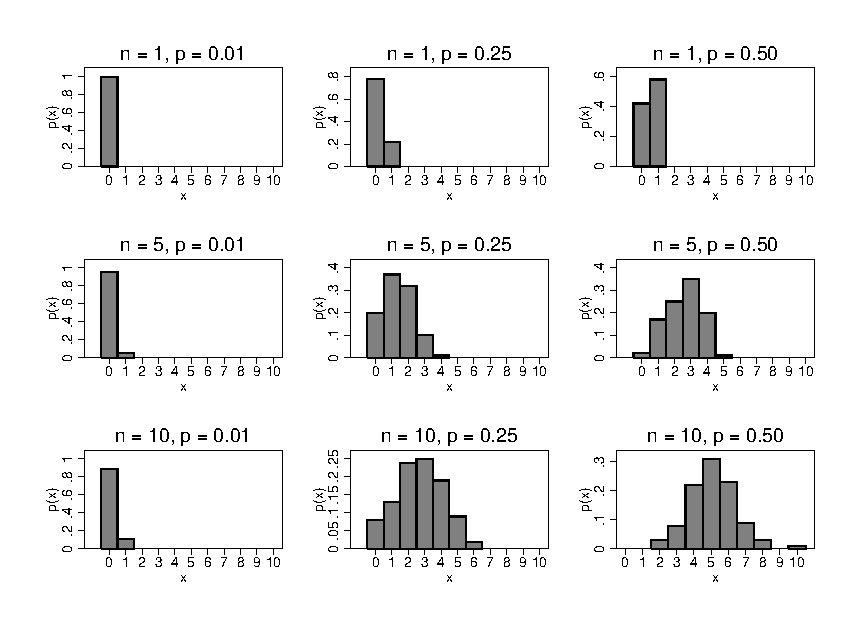
\includegraphics[angle=0,
           width=.75\textwidth]{binomial.eps}
   \caption{Distributions of random binomial variables with different values of $n$ and $p$.}
  \label{fig:binomial}
\end{figure}

\subsection{The Poisson distribution}
\label{sec:poisson}
The Poisson distribution is an extension of the binomial distribution. If we conceive of a parameter $\lambda = np$, where $n$ approaches infinity and $p$ approaches 0 (that is, the first couple trials have a high probability, but as trials increase the probability decreases), then this frequency distribution function becomes
\begin{equation}\label{eq:poisson}
P\left(X=k\right) = \frac{\lambda^k}{k!}e^{-\lambda}
\end{equation}
This distribution if often used to model count data.
\begin{figure}
   \centering
   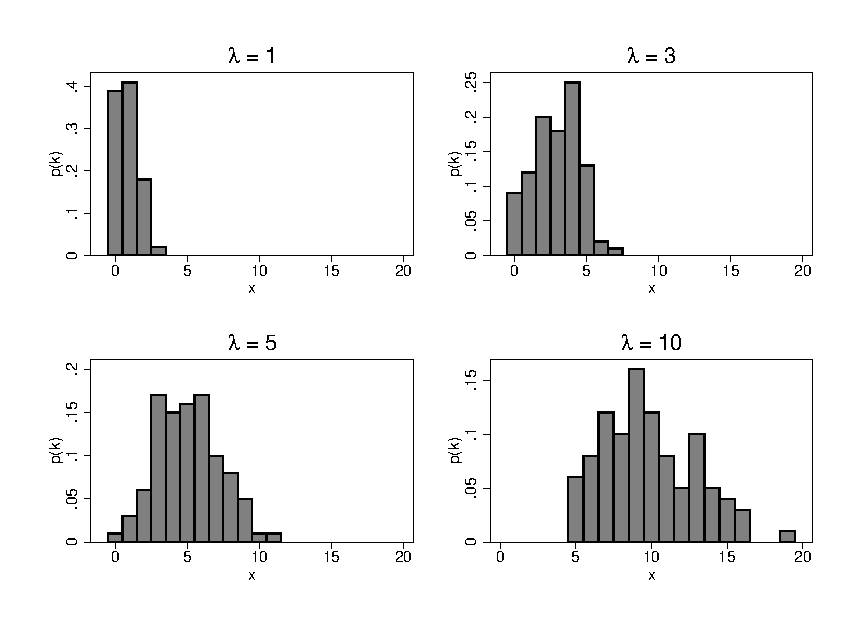
\includegraphics[angle=0,
           width=.75\textwidth]{poisson.eps}
   \caption{Distributions of random Poisson variables with different values of $\lambda$.}
  \label{fig:poisson}
\end{figure}

\subsection{Negative binomial distribution}
\label{sec:negbinomial}
We can extend the Bernoulli distribution to consider a series of Bernoulli events, each with a probability $p$, but ending after $r$ successes (or 1s). That is, out of $n$ times, how many instances are 0 or 1? The probability mass function of $k$ events to get $r$ successes is
\begin{equation}
\label{eq:negbinomial}
P(X=k) = {k-1 \choose r-1}p^r(1-p)^{k-r}
\end{equation}

\section{Continuous distributions}
\label{sec:condist}
The analogous idea to the probability mass function for discrete variables is the probability density function (PDF) that describes continuous variables. These functions have the property that the cumulation of all possible values equals 1. More importantly, we can find the probability that a variable has a value with the interval between $a$ and $b$ by integrating the function
\begin{equation}
P\left(a < X < b\right) = \int_a^b f(x)dx
\end{equation}
Of course, the chance of a specific value is 0
\begin{equation}
P\left(X = c\right) = \int_c^c f(x)dx = 0
\end{equation}
\subsection{The uniform distribution}

A useful distribution is the uniform distribution that spreads the chance of a variable falling between $a$ and $b$ evenly
\begin{equation}
f(x) = \frac{1}{b-a}
\end{equation}

\subsection{The normal distribution}
\label{sec:normaldist}
The big one is the normal distribution. We use this distribution (and others based on it) all statistical tests in regression. We define it with two parameters, $\mu$ and $\sigma$, or the mean and standard deviation.
\begin{equation}
f(x) = \frac{1}{\sigma\sqrt{2\pi}}\mbox{exp}\left[\frac{-\left(x-\mu\right)^2}{2\sigma^2}\right]
\end{equation}
The standard normal is shown in Figure~\ref{fig:normal}. A standard normal curve is one with $\mu = 0$ and $\sigma = 1$.

\section{Distributions based on the normal distribution}

From here, we move to the major distributions used for statistical tests. The central idea of such distributions is less about describing variables in data, but more describing the sampling distributions of statistics. We encounter these distributions when we consider the probability of observing a statistic (or the data that generated a statistic) assuming a specific null hypothesis in Chapter~\ref{sec:inference}. Note that some details, such as moment generating functions and the gamma distribution are left out, for more details, check out the mathematical statistics text in the bibliography.

\begin{figure}
   \centering
   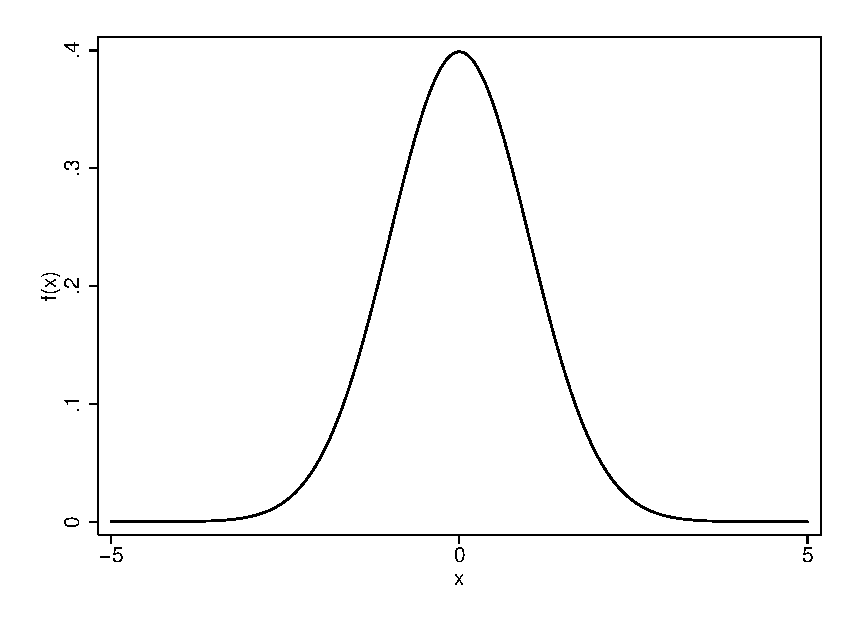
\includegraphics[angle=0,
           width=.75\textwidth]{normal.eps}
   \caption{A variable $x$ distributed $N \sim \left(0,1\right)$.}
  \label{fig:normal}
\end{figure}

\subsection{The $\chi^2$ distribution}

The $\chi^2$ distribution (written chi-square and rhymes with sky-square). This distribution (with 1 degree of freedom) is essentially the square of the normal distributions. That is, if $Z$ is standard normal, then $U = Z^2$ and $U$ is the $\chi^2$ distribution with 1 degree of freedom.

We note the distribution as $\chi_{df}^2$. We can take any normally distributed variable with mean $\mu$ and standard deviation $\sigma$ and transform it into a $chi_1^2$ by transforming it into standard normal and squaring it. That is, if
\[
X \sim N\left(\mu,\sigma\right)
\]
then
\[
\frac{X-\mu}{\sigma} \sim N\left(0,1\right)
\]
so
\[
\left(\frac{X-\mu}{\sigma}\right)^2 \sim \chi_1^2
\]
Formally, the $\chi^2$ distribution employs the gamma function ($\Gamma$) to find the density for any value ($v$) greater than 0 with a certain number of degrees of freedom ($df$):
\begin{equation}
f(v) = \frac{1}{2^{df/2}\Gamma\left(df/2\right)}v^{\left(df/2\right)-1}e^{-v/2}
\end{equation}
Finally, what really makes this distribution useful is that we can {\it add} independent variables' distributions and find the joint probability distribution (again, only if independent). Thus, if $U \sim \chi_n^2$ and $V \sim \chi_m^2$, then $U + V \sim \chi_{n+m}^2$. Thus, you will find many statistics used to evaluate aspects of a regression model will follow a $\chi^2$ distribution.

\begin{figure}
   \centering
   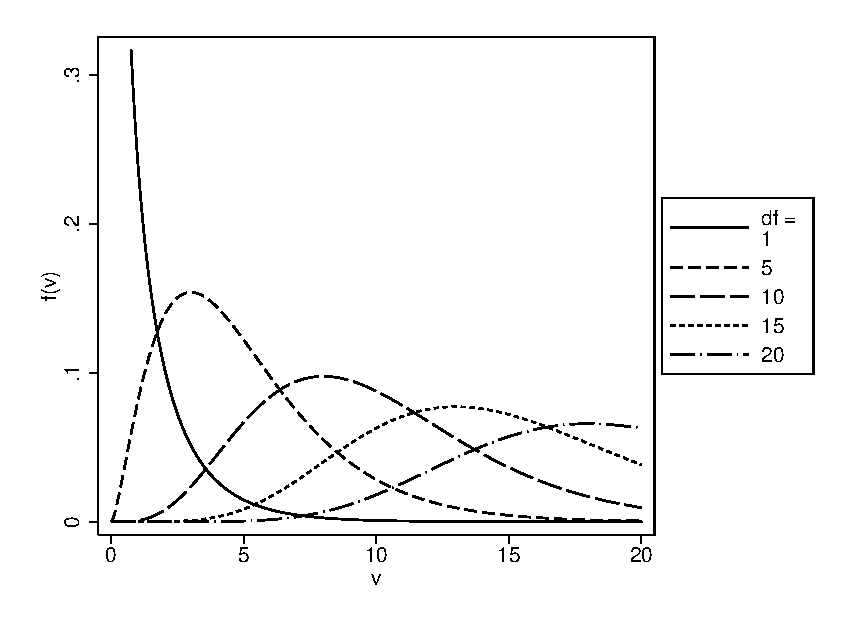
\includegraphics[angle=0,
           width=.75\textwidth]{chi.eps}
   \caption{Plot of $\chi^2$ distribution with various degrees of freedom.}
  \label{fig:chi}
\end{figure}

\subsection{The $t$ distribution}

The distribution you will encounter most often is the $t$ distribution, or sometimes called the "student's" $t$ distribution. This is not because a student derived it, far from it, but it was instead derived by a guy named Gossett in 1908 who was working for Guinness (as in beer) at the time, and published it under the pseudonym "student" for various reasons.

The $t$ distribution essentially works like the normal distribution, except it takes into account the small(er) sample sizes often used in research. If independent variables $Z \sim N\left(0,1\right)$ and $U \sim \chi_{df}^2$, then the $t$ distribution is the ratio of the normal $Z$ to the square root of the ratio of $\chi^2 U$ with $df$ degrees of freedom to $df$, or $t = \frac{Z}{\sqrt{U/df}}$.

Again, using the gamma function, this can we written as the following density function
\begin{equation}
f(t) = \frac{\Gamma\left(\frac{df+1}{2}\right)}{\sqrt{df\pi}\Gamma\left(\frac{df}{2}\right)}\left(1+\frac{t^2}{df}\right)^{\frac{-\left(df+1\right)}{2}}
\end{equation}

\begin{figure}
   \centering
   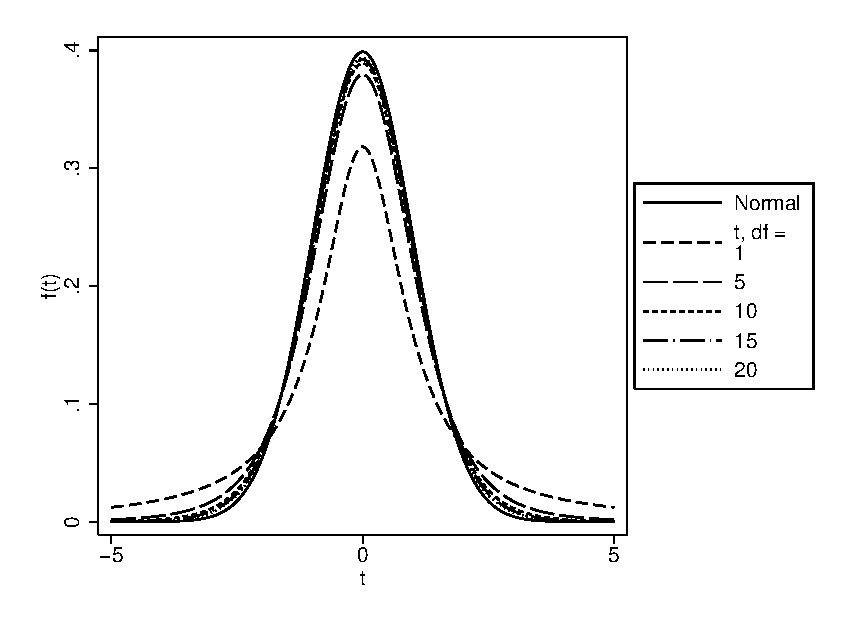
\includegraphics[angle=0,
           width=.75\textwidth]{tdist.eps}
   \caption{Plot of the normal distribution and two $t$ distributions with various degrees of freedom}
  \label{fig:tdist}
\end{figure}

\subsection{The $F$ distribution}

Finally, we have the $F$ distribution. If we have two independent $\chi^2$ variables, $U$ and $V$, distributed with $m$ and $n$ degrees of freedom respectively, then $F=\frac{U/m}{V/n}$, or formally for all positive values of $F$,
\begin{equation}
f(F) = \frac{\Gamma\left(\frac{m+n}{2}\right)}{\Gamma\left(\frac{m}{2}\right)\Gamma\left(\frac{n}{2}\right)}\left(\frac{m}{n}\right)^{\frac{m}{2}}F^{\frac{m}{2}-1}\left(1+\frac{m}{n}F\right)^{\frac{-\left(m+n\right)}{2}}
\end{equation}
\subsection{Who cares?}
There are several notable aspects of statistical analysis that make all these distributions based on the normal curve important. First, means and variances are independent with normally distributed variables, making modeling them in regressions very easy. Second, variances follow $\chi^2$ distributions, making the $F$-distribution appropriate for the ratio of variances.


\begin{figure}
   \centering
   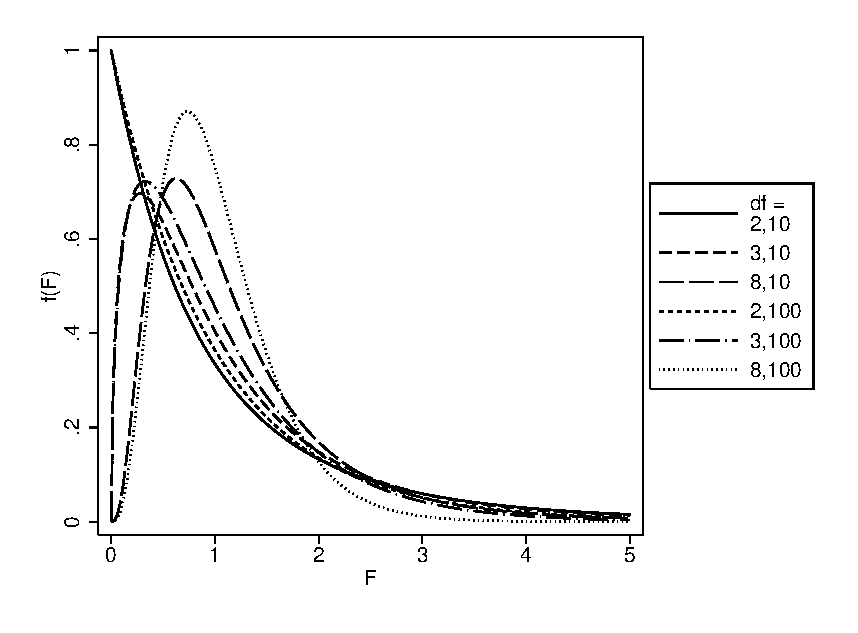
\includegraphics[angle=0,
           width=.75\textwidth]{f.eps}
   \caption{Plots of $F$ distribution with various degrees of freedom combinations.}
  \label{fig:f}
\end{figure}



\chapter{Basic Statistical Inference}\citep{cohen1988statistical}
\label{sec:inference}
\section{Sampling distributions}
Almost all the methods in these notes assume a simple random sample. {\bf If it is not a simple random sample, such as a two-stage cluster randomized sample from a major survey, these notes do not apply.} While the population mean, $\mu$, is fixed, the estimation of the mean, $\bar{x}$, is random because the selection of the sample is random. It therefore makes sense that if we were to gather another sample, that new sample's estimation of the mean will be different. This is the idea of sampling distributions: given a large number of samples, how will the estimate likely vary? What would the range of our estimate be 95 percent of the time?

\subsection{Basic principles of the central limit theorem}
If repeated random samples of size $N$ are drawn from any population with mean $\mu$ and standard deviation $\sigma$, as $N$ becomes large the sampling distribution of sample means will approach normality, with a mean of $\mu$ and standard deviation $\frac{\sigma}{\sqrt{N}}$.

There are two important parts here: that the mean of the sampling distribution should be close to the actual mean, and the standard deviation of the sampling distribution should be close to the standard deviation of the population divided by the square root of the sample size.

Keep in mind that the population distribution doesn't have to be normal--but the sampling distribution becomes normal with large N.

It is important to note that the central limit theorem suggests that the mean of our sample can be used as our guess of the population mean and we can quantify the uncertainly of this estimate with the variance of the estimates, of which the standard error is the square-root. This standard error is an estimate of the sampling distribution's standard deviation.

\section{The standard error of the mean}
Of course, it is extremely expensive to obtain repeated samples to get a good estimate of the mean. Researchers generally only have the resources for a single sample.

The formula for the standard deviation of samples of the a mean is similar to the standard deviation of the sampling distribution, except we substitute the population standard deviation, $\sigma$, with the estimate of the standard deviation from our sample, $s$. We start with the variance of the statistic, $\bar{x}$:
\begin{equation}
V\left(\bar{x}\right) = \frac{\sigma^2}{N}
\end{equation}
the square-root of which is the standard error
\begin{equation}
SE\left(\bar{x}\right) = \sqrt{\frac{\sigma^2}{N}}
\end{equation}
or the more familiar formula
\begin{equation}\label{eq:meanvar}
SE\left(\bar{x}\right) = \frac{\sigma}{\sqrt{N}}
\end{equation}
and our estimate of this replaces $\sigma$ with $s$
\begin{equation}
SE\left(\bar{x}\right) = \frac{s}{\sqrt{N}}
\end{equation}
This gives us the "variance" of our mean estimate. All statistics have "variances" associated with them. Much of the more advanced statistics and sample statistics that are taught in graduate schools focus on getting the right variances, and thus the right standard errors. Much the time, the formulas of the point estimates (the statistics) are pretty much the same.

\section{The standard error of a proportion}
The variance of a mean for linear variables is not direct a function of the value of the mean, it just depends on the standard deviation. In the case of proportions, the variance is a function of the estimate itself:
\begin{equation}\label{eq:par}
\sigma^2_p=p\left(1-p\right)
\end{equation}
This is true because if $p$ is the mean and $x_i$ only takes on values of 0 or 1, then $Np$ is the number of observations in which $x_i=1$ and $N\left(1-p\right)$ is the number of observations in which $x_i=0$. Thus, the variance (without the sample correction of $N-1$ for $N$) can be calculated as
\begin{equation}
s^2 = \frac{\sum_{i=1}^N\left(x_i - p\right)^2}{N} = \frac{Np\left(1-p\right)^2 + N\left(1-p\right)p^2}{N} = \frac{Np\left(1-p\right)}{N} = p\left(1-p\right)
\end{equation}
What is calculated by computers is this times $\frac{N}{N-1}$ to get an unbiased estimate of the population variance, but for large $N$ this is close to 1.
So, the standard error of the proportion is a function of the proportion itself:
\begin{equation}
SE\left(p\right) = \sqrt{\frac{N}{N-1}\times\frac{p\left(1-p\right)}{N}}
\end{equation}
\section{Hypothesis testing}
So now that we have an estimate of the mean, and a sense of our uncertainty about this estimate, we can now ask a theoretical question: let's say we did draw several samples from the population, what is the range for 95 percent of the means we would get? We can do this by calculating a confidence interval of the estimated statistic. Confidence intervals generally take the form of
\begin{equation}
CI\left(\theta,\left(1-\alpha\right)\times100\right)=\hat{\theta}\pm t_{df,\alpha/2}SE\left(\hat{\theta}\right)
\end{equation}
Where $\theta$ is the parameter of interest, $\hat{\theta}$ is the statistic that estimates the parameter, $SE\left(\hat{\theta}\right)$ is the standard error of that statistic, $\alpha$ is the Type I error rate, and $t$ is the critical value of the $t$-distribution associated with the $df$ degrees of freedom of the statistic and the Type I error rate. As you can see in Figure~\ref{fig:tdist}, the $t$ distribution is similar to the $Z$ distribution except that it has slightly different shapes for different degrees of freedom.

In this case, the parameter of interest is the population mean, $\mu$. We are estimating that with the sample mean statistic, $\bar{y}$ . Note that we are now talking about a variable $y$ instead of $x$, this is because we are transitioning from any old variable to outcomes, which are typically represented with the variable $y$. For that statistic, we also have a standard error $SE\left(\bar{y}\right)$.

In the social sciences, the common Type I error rate is 5 percent, or $\alpha = 0.05$. What is the Type I error rate? Type I error is the chance of falsely rejecting the hypothesis that the true parameter could fall outside the confidence interval. In other words, if we are going to make the assertion that some other parameter, $\theta_{null}$, is different than our population parameter, $\theta$, for which we have a sample estimate, $\hat{\theta}$, we want there to be only a $\left(1-\alpha\right)\times100$ percent chance of being wrong.

Finally, we need to scale our standard error by something to create the confidence interval. Since the sampling distribution is normal with a standard deviation of $SE\left(\hat{\theta}\right)$, we want to form our confidence interval so that it gives us the bounds of percent of the possible sample estimates.

One option is to use the normal $Z$ distribution, in which case, for example, a 95 percent confidence interval (meaning that $alpha = 0.05$) is bounded by -1.96 and 1.96. However, we typically use the $t$-distribution rather than the normal distribution because it "flattens out" as the sample size gets small, making the confidence intervals wider (see Figure~\ref{fig:tdist}). Thus, in order to get the right number from the $t$-distribution, we need to know the degrees of freedom, which in a one sample case is $N - 1$. Thus, confidence intervals for smaller samples will always be larger. They are larger for two reasons. First, if we look at the formula for a standard error,
\begin{equation}
SE\left(\bar{x}\right) = \frac{s}{\sqrt{N}}
\end{equation}
we see that the denominator is essentially the sample size. Smaller samples, larger standard errors. The second reason is that we use the sample size to determine the degrees of freedom when selecting the value from the $t$ distribution. Smaller samples, larger values of $t$ for any given $\alpha$.

Why do we care about this? We care because we may want to make an assertion that the estimated parameter, $\hat{\theta}$, is different from some other value, $\theta_{null}$. If $\theta_{null}$ is outside the confidence interval, then the estimate is statistically different. Another way is to find the difference between $\hat{\theta}$ and $\theta_{null}$, and divide by $SE\left(\hat{\theta}\right)$. This gives you the value of $t$ for a confidence interval, and you can compare it to the $t$ you would use to construct a confidence interval, or the critical $t$. If
\begin{equation}
\frac{\hat{\theta}-\theta_{null}}{SE\left(\hat{\theta}\right)}>t_{critical, df, \alpha/2}
\end{equation}
then the estimate is statistically different.

Can we be absolutely sure? No, because our confidence interval only covers $\left(1-\alpha\right)\times100$ percent of the sampling distribution, another sample could have given us a different answer.

This is all backing into hypothesis testing. We could play this game all day of calculating confidence intervals and seeing if some arbitrary value falls within the bounds. A much simpler approach is to do a hypothesis test.

Most stats text books will tell you that there are 5 steps to doing a hypothesis test that include making an assertion of our Type I error we assume, stating the critical value, etc. I think these steps are silly, since no one ever does these steps in discrete order. This is how it is done in practice.
We typically think of $\theta_{null}$ as the null hypothesis (or the value of the parameter or model we will assume to be true). We can write the null hypothesis like this (in terms of the population parameter $\theta$:
\[
H_0:\theta=\theta_{null}
\]
where we say that the population parameter, $\theta$, is equal to the null value, $\theta_{null}$.
The alternative hypothesis is that these values are unequal
\[
H_1:\theta\ne\theta_{null}
\]
First, we calculate our test statistic. Test statistics for parameters that use the $t$-distribution generally take the form of
\begin{equation}
t = \frac{\hat{\theta}-\theta_{null}}{SE\left(\hat{\theta}\right)}
\end{equation}\label{eq:ttest}
for $t$-tests when we have a specific degrees of freedom, or
\begin{equation}\label{eq:ztest}
z = \frac{\hat{\theta}-\theta_{null}}{SE\left(\hat{\theta}\right)}
\end{equation}
for $z$ tests when there are no real degrees of freedom to consider.

Basically, what we are doing is calculating the difference between what we estimated and what we assume is true (the null hypothesis) and then we divide that difference by the standard error of our estimate.

We then look up the probability of that test on the appropriate distribution associated with the statistic and degrees of freedom. If that probability is less than 0.05, then we say we can reject the null. I do not talk about one-tail tests.

A probability less than 0.05 means that what we get from our sample is highly unlikely if we assume the null hypotheses, so we can then reject the null hypothesis. There is still a chance that the null is correct and we got a weird sample, that's our Type I error rate, but we feel that 5 percent or less is acceptable.

\subsection{What is a $p$-value?}

When you have a result from one of the major distributions ($Z$, $\chi^2$, $t$, or $F$) and the associated degrees of freedom (if applicable), you can generate a $p$-value. $p$-values allow us to estimate the smallest $\alpha$ could be for a given hypothesis test to be rejected. If the $p$-value is greater than 0.05, generally, you have to accept the null. We use $p$-values mainly because of Fisher, who thought of them as the probability under the null hypothesis of a result as, or more extreme, than the data.

\subsection{Comparing two means}
\label{sec:pooled}
I really do not see many comparisons between a population mean and some other value. What I do see a lot of are comparisons between two groups that are sampled independently. We should be careful when we think about this, because in observational studies like the General Social Survey, we do not sample Republicans separately from Democrats. We randomly sample the population, and some are Republicans and some are Democrats. Even in experiments, we randomly sample a group then randomly assign treatment or control.

Regardless, we always talk about testing two independent means, for example between groups A and B. They are independent because the observations from group A are in no way related to observations from group B. However, we are not really dealing with a test of two statistics, we are estimating a single statistic, {\it the difference}. In population terms, this is
\[
\theta=\mu_A-\mu_B,
\]
and from our sample estimates it is
\[
\hat{\theta}=\bar{y}_A-\bar{y}_B.
\]
We then state the null hypothesis as this difference being 0 (i.e., $\theta_{null} = 0$) as
\[
H_0:\theta=\theta_{null}
\]
\[
H_0:\mu_A-\mu_B=0
\]
and the alternative hypothesis as
\[
H_1:\mu_A-\mu_B\ne0.
\]
In the case of independent means, we can estimate the standard error of this difference using a pooled standard deviation
\begin{equation}
SE\left(\bar{y}_A-\bar{y}_B\right)=\frac{s_{pooled}}{\sqrt{N}}
\end{equation}
where
\begin{equation}
s_{pooled} = \sqrt{\frac{\left(n_A-1\right)s_A^2+\left(n_B-1\right)s_B^2}{n_A+n_B-2}}.
\end{equation}
The $t$ test is then
\begin{equation}
t = \frac{\bar{y}_A-\bar{y}_B}{SE\left(\bar{y}_A-\bar{y}_B\right)}
\end{equation}
We then evaluate the value of $t$ against some level of $\alpha$ using $N-2$ degrees of freedom.

If there is a relationship between groups A and B, like one "group" was a set of pre-tests and the second "group" was a set of post tests, each pre-test and post-test was from the same set of people, then we would be doing a paired t-test. In this case the test is
\begin{equation}
t=\frac{\bar{d}\sqrt{N}}{s_d}
\end{equation}
where
\begin{equation}
\bar{d} = \frac{\sum_{i=1}^N\left(y_{Ai}-y_{Bi}\right)}{N}
\end{equation}
and
\begin{equation}
s_d = \sqrt{\frac{\sum_{i=1}^N\left(\left(y_{Ai}-y_{Bi}\right)-\bar{d}\right)^2}{N-1}}
\end{equation}
with $N$ pairs of values. The test is then evaluated against the $t$ distribution using $N-1$ degrees of freedom.

\section*{For more information}
For statistical power analysis, see \citep{cohen1988statistical} and \citep{aberson2011applied}. For sample size planning, consult \citep{maxwell2008sample}. Foundational material on statistical inference can be found in \citep{rice2007mathematical} and \citep{agresti}.




\chapter{Basic multivariate analyses}

\section{The analysis of variance (ANOVA)}
When we are considering three or more groups, we ask whether these groups are different from each other. Another way to think about this is to think about how much of the variance occurs between the groups compared to how much variance occurs within the groups. This ratio is the idea behind ANOVA.

The building blocks of ANOVA is that we can think about each $i^{th}$ case as part of the $j^{th}$ group. We can then conceptualize a way to think about deviance that involves groups.

Here, we can think of the total difference between an observation and the overall mean, $y_{ij}-\bar{y}$, as the difference between that observation and its group's mean, $y_{ij}-\bar{y}_j$, plus the difference between that group's mean and the overall mean, $\bar{y_{j}}-\bar{y}$:
\begin{equation}
y_{ij}-\bar{y} = \left(y_{ij}-\bar{y}_j\right)+\left(\bar{y_{j}}-\bar{y}\right)
\end{equation}
This idea has implications for the sum of squares. We can now think of the total sum of squares ($SST$) as breaking down into the sum of squares within groups ($SSW$) and the sum of squares between groups ($SSB$):
\begin{equation}
SST=SSW+SSB
\end{equation}
or
\begin{equation}
\sum_{j=1}^k\sum_{i=1}^{n_j}\left(y_{ij}-\bar{y}\right)^2=\sum_{j=1}^k\sum_{i=1}^{n_j}\left(y_{ij}-\bar{y}_j\right)^2+\sum_{j=1}^kn_j\left(\bar{y}_j-\bar{y}\right)^2
\end{equation}
There is some new notation here. We now have $k$ groups with the subscript $j$, and each $j^{th}$ group has cases with the subscript $i$.

ANOVA's test statistic relies on the F-distribution to evaluate Type I error. The F-distribution is used to test ratios and is thus defined by two degrees of freedom, one for the numerator and one for the denominator of the ratio, and there are no negative statistics.  As the number of each increases to a large number, the distribution starts to look normal.

As was just mentioned, the test statistic is a ratio. Again, we are concerned with the ratio of the variance that occurs between groups compared to that within groups. Thus, this ratio uses as the numerator the mean square between, which is the sum of squares between divided by the number of groups - 1:
\begin{equation}
MSB=\frac{\sum_{j=1}^kn_j\left(\bar{y}_j-\bar{y}\right)^2}{k-1}
\end{equation}
The denominator of the ratio is the mean square within, which is the sum of squares within divided by the number of cases minus k group means
\begin{equation}
MSW=\frac{\sum_{j=1}^k\sum_{i=1}^{n_j}\left(y_{ij}-\bar{y_{ij}}\right)^2}{N-k}
\end{equation}
The ratio then looks like this
\begin{equation}
F=\frac{MSB}{MSW}
\end{equation}
and we test how much of the $F$-distribution (with $k$ and $N-k$ degrees of freedom) is left after this value for our Type I error rate of our test of the the null hypothesis that all group means are the same. In other words, our null hypothesis is that all the group means are the same:
\begin{equation}
H_0:\mu_1=\mu_2 \ldots =\mu_k.
\end{equation}
Since this distribution has two degrees of freedom parameters, the critical value different for different combinations of $k$ and $N-k$. See Figure~\ref{fig:f} for various distributions.

\subsection{ANOVA Example}

As a cartoony example, let's use political views to predict vocabulary. Or, in less causal language, whether vocabulary varies by political view. These data come from the General Social Survey.

First, we have three political groups, liberal (lib), moderate (mod), and conservative (con). Summary statistics appear in Table~\ref{tab:polstats}.
\begin{table}[htbp]\centering
\caption{Number correct words by political affiliation\label{tab:polstats}
\textbf{} }\begin{tabular} {@{} l r r r @{}} \\
Political affilication &     $N$ & $\bar{y}$ &  $s$ \\
\hline
   lib &   733 &    6.32 &    2.21 \\
   mod &   983 &    5.81 &    1.84 \\
   con &   875 &    6.23 &    1.97 \\
   \hline
  Total &  2591 &    6.10 &    2.01 \\
\hline
\multicolumn{4}{@{}l}{\footnotesize{\emph{Source: General Social Survey: 2008}}}
\end{tabular}
\end{table}

Table~\ref{tab:wordanova} is a typical ANOVA table with the total sum of squares broken down into the sum of squares within and between, with the mean squares also calculated. We can calculate the $F$-test using the mean squares
\[
F=\frac{MSB}{MSW}=\frac{67.216}{3.984}=16.87.
\]
Which, evaluated with $\left(2,2588\right)$ degrees of freedom on the $F$ distribution, has a probability of 0.0000005. This indicates that at least one group is different than the others. To find out which group is different requires some regression analysis.

\begin{table}[htbp]\centering
 \caption{ANOVA of word test by political views
\label{tab:wordanova}}
\begin{tabular}{lrrr}
\hline
Source & Sum of squares & $df$ & Mean Squares \\
\hline
Between groups & 134.432 & 2 & 67.216 \\
Within groups & 10311.878 & 2588 & 3.984 \\
\hline
Total & 10446.31 & 2590 & 4.03 \\
\hline
\multicolumn{4}{l}{Model Statistics} \\
\hline
$N$      &   2591 & \\
$F$      &   16.87  \\
\hline
\end{tabular}
\end{table}

\section{Covariance}
The covariance is a simple idea: instead of squaring the deviance of one variable from its mean, the covariance multiplies the deviances of two variables from their means:
\begin{equation}
  \mbox{cov}\left(y,x\right)=\frac{\sum_{i=1}^N\left(y_i-\bar{y}\right)\left(x_i-\bar{x}\right)}{N-1}
\end{equation}
\begin{table}[htbp]\centering
\caption{Small dataset of random variables\label{tab:xy}
\textbf{} }\begin{tabular} {@{} c c @{}} \\
$y$ & $x$ \\
\hline
 8.20&4.51\\
 9.21&5.36\\
10.22&6.23\\
 8.56&3.84\\
10.66&4.90\\
 9.93&5.00\\
 8.29&4.80\\
 9.18&4.34\\
 9.22&5.78\\
 7.29&4.06\\
\hline
\multicolumn{2}{@{}l}{\footnotesize{\emph{} }}
\end{tabular}
\end{table}
\begin{figure}
   \centering
   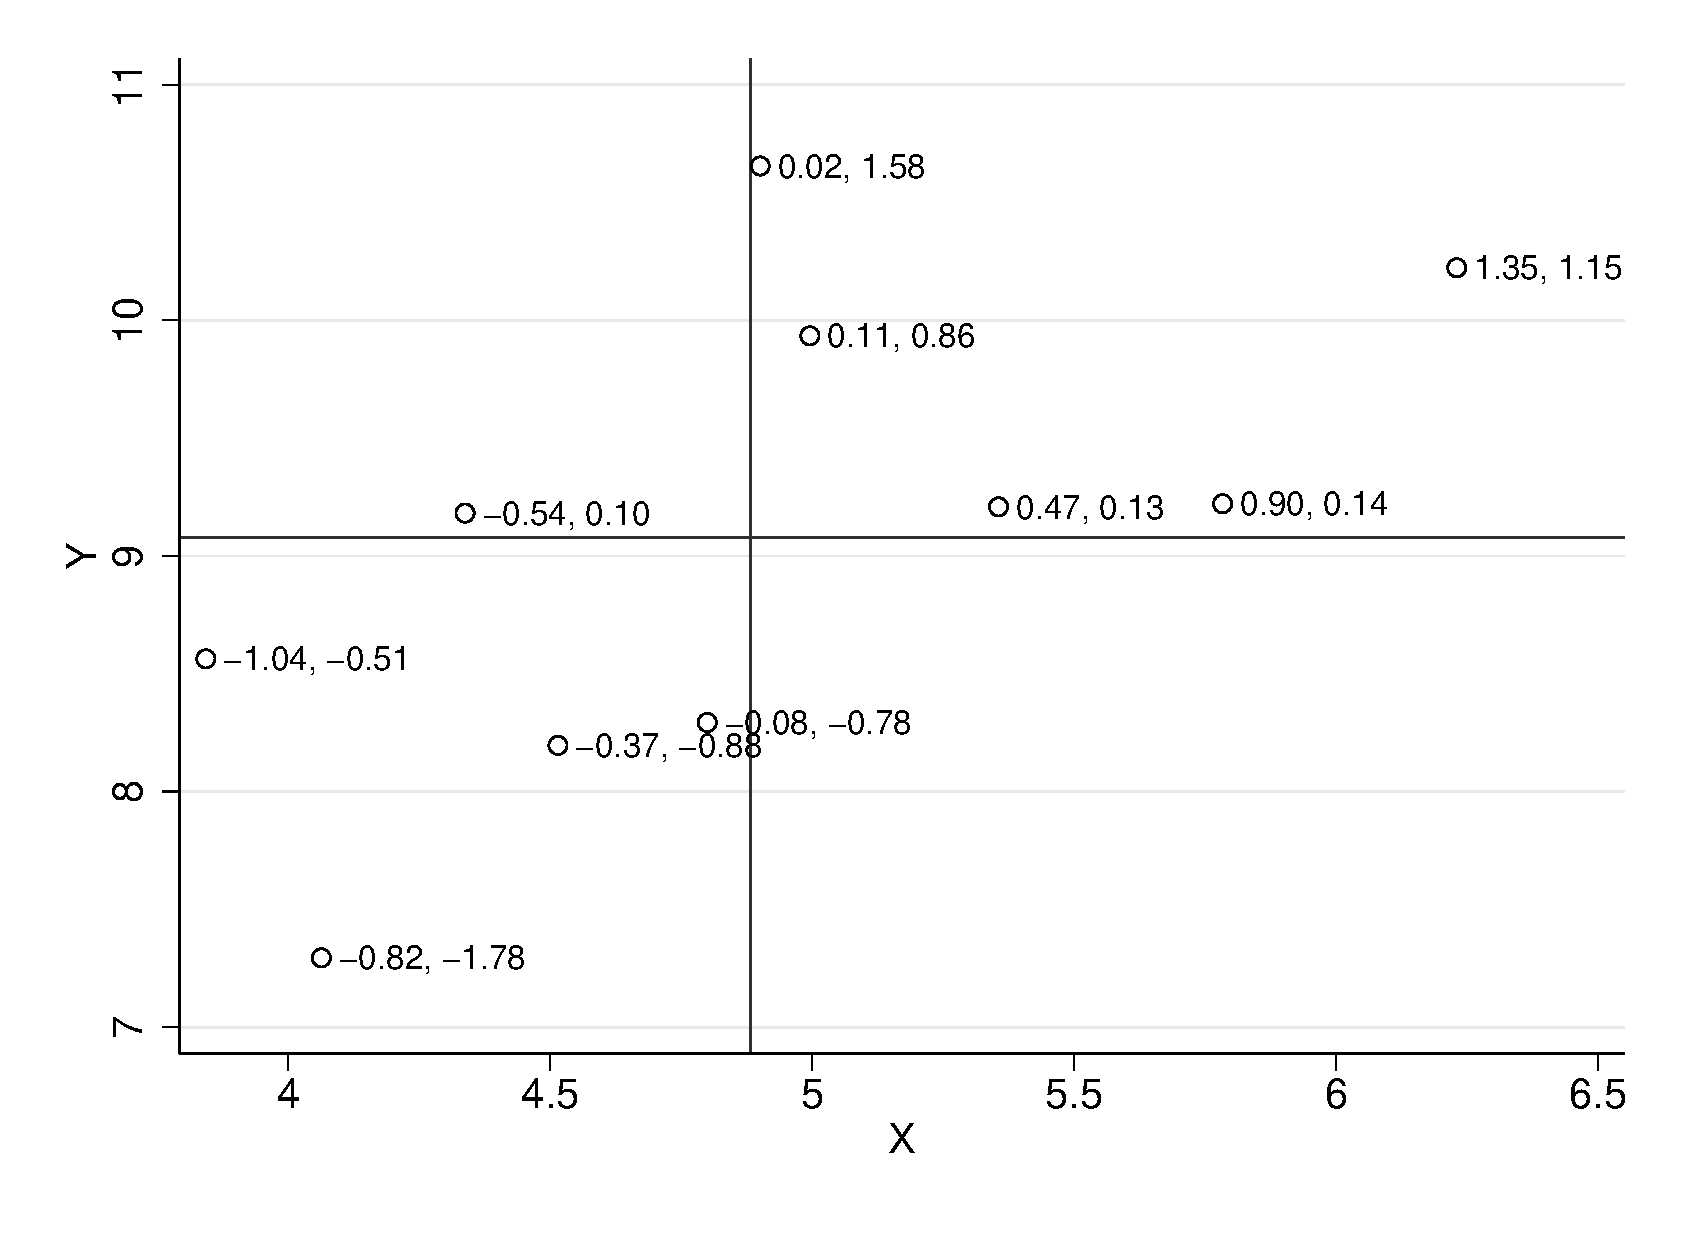
\includegraphics[angle=0,
           width=.75\textwidth]{cov_xy.eps}
   \caption{Plot of variables $y$ and $x$ with solid lines for means, labeled with deviations from the means}
  \label{fig:cov_xy}
\end{figure}
We can visualize this by using a scatterplot. Figure~\ref{fig:cov_xy} is a scatterplot of the data with the means of $x$ and $y$ marked with vertical and horizontal lines and each point marked with the deviations from the mean. The data appear in Table~\ref{tab:xy}.
\begin{figure}
   \centering
   \includegraphics[angle=0,
           width=.75\textwidth]{cov.eps}
   \caption{Covariance quadrants}
  \label{fig:cov}
\end{figure}
Now, consider Figure~\ref{fig:cov}. The means of $x$ and $y$ have been graphed into four quadrants. Each quadrant is defined by the sign of the deviation from the means of $x$ and $y$. Observations whose values of $x$ and $y$ are both larger than the mean of $x$ and $y$ respectively will fall into quadrant one $(+,+)$. Observations whose values have $x$ and $y$ are both lower than the respective means will fall into quadrant three $(-,-)$. The key is that the product of any deviations in either of these quadrants will be positive (a negative times a negative is positive). On the other hand, points that fall into the other quadrants (quadrant two and quadrant four) will have products that are negative (a negative times a positive is negative).

Why do we care about the products of the deviations? Consider the numerator of the covariance formula, $\sum_{i=1}^N\left(y_i-\bar{y}\right)\left(x_i-\bar{x}\right)$. All this is doing is adding up these products. Therefore, more positive products will produce a large positive number, more negative products will produce a large negative number. In addition, larger deviations of either $x$ or $y$ will create larger numbers, and large deviations of both $x$ and $y$ will create a really big number.

If more points fall into the positive quadrants $(+,+; -,-)$ the result is a positive number. If more points fall into the negative quadrants $(-,+;+,-)$, the result is negative. If equal numbers fall into each quadrant, then they will balance out and the number will be close to 0.

Figure~\ref{fig:cov_xy} shows the deviations marked for each point on the scatterplot: what do you think the covariance is?

The denominator of the covariance formula ($N-1$) just turns it into an average, like the variance. Looking at Figure~\ref{fig:cov_xy}, we can tell that the relationship between $x$ and $y$ is positive. The direction of a relationship is generally thought of as what happens to $y$ as $x$ increases. Thus, the covariance in Figure~\ref{fig:cov_xy} is 0.47. This tells me that when $x$ increases, so does $y$. If this number was negative, then as $x$ increases $y$ would decrease.
\section{Correlation}
One of the biggest problems with covariance is that it is really hard to interpret anything meaningful from it. Covariance identifies if the relationship is positive or negative, but it doesn't provide information about the magnitude of the relationship. In addition, the units get all messy. For instance, if the variables were wages and years of education, then the units would be wage-years. What is a wage-year? The solution to this problem is standardization. It would be helpful to standardize this quantity, and one method is to use the sum of squares of the two variables involved. This is basically what the correlation coefficient is about. It is a standardized covariance. The correlation formula is
\begin{equation}
  r_{y,x}=\frac{\sum_{i=1}^N\left(y_i-\bar{y}\right)\left(x_i-\bar{x}\right)}{\sqrt{\sum_{i=1}^N\left(y_i-\bar{y}\right)^2\sum_{i=1}^N\left(x_i-\bar{x}\right)^2}}
\end{equation}
The numerator of this equation is simply the covariance formula while the denominator is the sum of the squares equation. Since the units of the variables are the same for the numerator and denominator, the units cancel out

Correlation coefficients range from -1 to 1. If it is 0, it means that there is no covariance between $x$ and $y$. If it is close to 1, it means that there is a strong positive covariance between $x$ and $y$. If it close to -1, it means that there is a strong negative covariance between $x$ and $y$. All information about the units is lost. It does not matter what $x$ and $y$ are measured by.
\subsection{Testing the correlation coefficient}
\label{sec:introhypo}
What if we wanted to know if our correlation coefficient was {\it statistically} different than 0? In this case, we need to consider the sampling distribution of the correlation coefficient. I go into this in more detail below, but for now remember that we have a random {\it sample}, and if we started our research another day, we would get a different {\it sample}. Thus, the estimated correlation coefficient from our data is one of many possible estimates. We want to know the distribution of these estimates from different hypothetical samples, so we can know how likely our estimate is, assuming a world where a null hypothesis is true. In this case, our null hypothesis is that there is no correlation. For the data in Figure~\ref{fig:cov_xy}, the correlation is 0.61. The question is, is this statistically different than 0?

Since we have a sample, we will rely on the student's $t$ distribution. We can estimate a test statistic for a correlation with
\begin{equation}
t = \frac{|r|\sqrt{N-2}}{\sqrt{1-r^2}}
\end{equation}
which in this case is
\[
t = \frac{0.61\sqrt{10-2}}{\sqrt{1-0.61^2}}
\]
\[
t = 2.18
\]
Now, in our case in Table~\ref{tab:xy}, we have 10 cases, and with 2 means (for two variables) we have 10-2 = 8 degrees of freedom. Figure~\ref{fig:critical} is the sampling distribution of our statistic if we assume that the null hypothesis, or the hypothesis that the correlation is 0, is true. If you look carefully, you will see that the probability of finding a correlation of 0.61 with 10 cases is about 0.06. The math to find that number is a little tedious, so most stats books tell you what test you need to get in order to have a sufficiently low probability to reject the null hypothesis. In our case, that value is about 2.31. Why 2.31? That is a number large enough to claim that if we assume the null hypothesis, the chance of finding that test in our data is less than 0.05. Another way of saying that is that the Type I error rate is less than 5 percent. We sometimes call the Type I error rate $\alpha$ and so we say that $\alpha = 0.05$.

In this case, with a test statistic of 2.18, which is smaller than the critical value of 2.31, we have to accept the null hypothesis. It was close, but not enough.
\begin{figure}
   \centering
   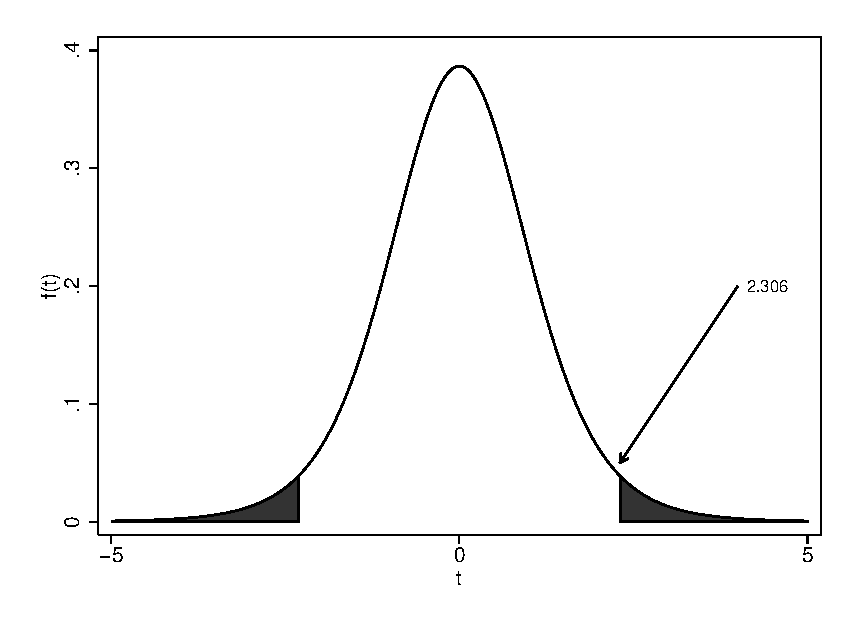
\includegraphics[angle=0,
           width=.75\textwidth]{critical.eps}
   \caption{Plot of $t$ distribution with 8 degrees of freedom and $\alpha$ = 0.05 critical tails marked.}
  \label{fig:critical}
\end{figure}

\section{Chi-square}
In the case of two categorical variables, neither covariance or correlation should be used to determine relationships. Instead, another method based on the idea of deviation is appropriate; the Chi-square $\left(\chi^2\right)$ test. The idea is to state a "null" hypothesis in terms of the researcher's expectation for the results of their analysis. The researcher states what she/he expects, and then offer an alternative hypothesis. If the data deviates in a substantial degree from what the researcher "expects," then the researcher must "fail to reject" the null hypothesis. In common practice, a null hypothesis indicates that there will be no statistically significant relationship between two variables while the alternative hypothesis indicates that there is a statistically significant relationship between the two variables.

The trick to Chi-square tests is that the "expected" value can be anything. You may remember the Chi-square tests from your research methods or statistics class. Frequently, data is presented in table format. In such a table we have (at least) two categorical variables $x$ and $y$. The variable $x$ takes on values such as $x\in\left\{1 \ldots i\right\}$ and variable $y$ takes on values such as $y\in\left\{1 \ldots j\right\}$. Each cell in the table has a number of observations associated with it, $n_{ij}$, for a total of $N=\sum_i\sum_jn_{ij}$ observations. In the case of a two variable table, $x$ makes up the rows and $y$ makes up the columns. We also have totals for each row, $n_{i+}$, and for each column, $n_{+j}$. Chi-square tests then make a comparison between the observed frequency, $n_{ij}$ and what the researcher "expects" each cell frequency to be, $m_{ij}$. This test is
\begin{equation}
\chi^2=\sum_i{\sum_j{\frac{\left(n_{ij}-m_{ij}\right)^2}{m_{ij}}}}.
\end{equation}
A big value for this number tells us that there is a difference between our data and our expectation. Depending on what we are doing, this expectation is different. If we are testing to see if two variables are independent, when we test against a random expectation, or we expect the cells to simply be a function of the margins. So, in this case, $m_{ij}$ is
\begin{equation}
m_{ij}=\frac{n_{i+}n_{+j}}{N}
\end{equation}
So, what's a big value? In this case, it depends on how many cells are in the table. Any statistical test is compared to a function, generally based on some degrees of freedom. For example, a Chi-square test is compared against a Chi-square distribution with $\left(rows-1\right)\left(columns-1\right)$ degrees of freedom. If the value of the test is far enough along that distribution to be considered unlikely if the expectation is true, then we reject the expectation. For example, a $2\times2$ table has a single degree of freedom and a critical value of 3.84 for a Type I error rate of 0.05. Figure~\ref{fig:chi} display some $\chi^2$ distributions.



\chapter{Least squares and maximum likelihood}
\section{The mean}\label{sec:mean}
\subsection{Least squares}
These notes are for regression. So now is the time to know that regression produces a conditional mean (a mean that exists under certain specified conditions). Since learning regression is what we are here to do, it makes sense to show how useful means really are. If we use as our criteria for whether a summary statistic about the data is "good" or not is the deviation between the observation and our statistic, then we want a summary statistic to minimize these differences.

As mentioned earlier, adding up all of the deviances will produce 0. To circumvent this problem, the deviances were squared and then added up. Therefore, we want our mystery statistic, $\theta$ to be a {\it function} of these squared deviations:
\begin{equation}
S\left(\theta\right)=\sum_{i=1}^{N}e_i^2=\sum_{i=1}^{N}\left(x_i-\theta\right)^2
\end{equation}
A "good" estimate will have the least amount of differences. Thus, we want our statistic to minimize $\sum_{i=1}^{N}\left(x_i-\theta\right)^2$. So, how to we figure out which statistics will minimize the sum of these squared deviations? Let's break it down into known and unknown quantities. Someone smarter than me figured out that if you rearrange the terms, you can express this function as
\[
S\left(\theta\right)=\sum_{i=1}^{N}\left(x_i-\theta\right)^2
\]
factor it
\[
S\left(\theta\right)=\sum_{i=1}^{N}\left(\left(x_i-\theta\right)\left(x_i-\theta\right)\right)
\]
\[
S\left(\theta\right)=\sum_{i=1}^{N}\left(x_i^2-x_i\theta-x_i\theta+\theta^2\right)
\]
\[
S\left(\theta\right)=\sum_{i=1}^{N}\left(x_i^2-2x_i\theta+\theta^2\right)
\]
then take the elements out of the summation
\begin{equation}
S\left(\theta\right)=\sum_{i=1}^{N}x_i^2-2\theta\sum_{i=1}^Nx_i+N\theta^2
\end{equation}
Since, theoretically, we know our data, and thus know the sum of x squared, $\sum_{i=1}^{N}x_i^2$ , and the sum of x, $\sum_{i=1}^{N}x_i$, and $N$, then this function only has one unknown, $\theta$. We can use calculus to find the first derivative of this function with respect to $\theta$. Relying on the fact that the derivative of a sum of functions is the sum of the derivatives of each function, we can find the derivative of each element. The derivative of $\sum_{i=1}^{N}x_i^2$ is 0, since it is a constant and doesn't involve $\theta$, the derivative of $-2\theta\sum_{i=1}^Nx_i$ with respect to $\theta$ is $-2\sum_{i=1}^Nx_i$, and finally the power rule tells us that the derivative of $N\theta^2$ is $2N\theta$. Adding this all together gets us the derivative of the function with respect to $\theta$ as
\begin{equation}
\frac{dS\left(\theta\right)}{d\left(\theta\right)}=-2\sum_{i=1}^{N}x_i+2N\theta
\end{equation}
Then we set this first derivative to 0 (the first derivative of a function is its slope, and when the slope of a function is zero, the function is at a minimum or maximum) and solve for $\theta$:
\[
0=-2\sum_{i=1}^{N}x_i+2N\theta
\]
\[
2\sum_{i=1}^{N}x_i=2N\theta
\]
\[
\sum_{i=1}^{N}x_i=N\theta
\]
\[
\frac{\sum_{i=1}^{N}x_i}{N}=\theta
\]
Now that we have it, we name the statistic $\mu$ and also call it the mean, c.f.~\eqref{eq:mean}. For example, Table~\ref{tab:desx} presents some random numbers and the key statistics to graph the least squares function. For Table~\ref{tab:desx} this function is
\[
S\left(\theta\right)=\sum_{i=1}^{N}x_i^2-2\theta\sum_{i=1}^{N}x_i+N\theta^2
\]
\[
S\left(\theta\right)=9887.521-2\theta 988.596+N\theta^2
\]
and this function is visualized in Figure~\ref{fig:sse}. I show that the mean we estimate does indeed present the minimum sum of squared errors. Any other value for the mean increases error.

\begin{table}[htbp]\centering
\caption{Random variable $x$\label{tab:desx}
\textbf{} }\begin{tabular} {@{} ccccc @{}} \\
\hline
10.939&10.470&10.333&8.738&9.827 \\
10.279&9.754&10.261&11.036&10.054 \\
10.637&10.659&10.742&10.492&11.260 \\
10.378&9.007&10.092&9.430&10.618 \\
8.147&10.414&10.250&9.378&9.728 \\
10.338&8.780&10.539&10.504&8.474 \\
8.430&10.244&11.622&9.584&10.187 \\
8.431&9.532&9.669&9.460&9.913 \\
7.349&9.671&10.607&9.558&10.503 \\
9.519&9.866&9.010&9.059&8.804 \\
9.709&9.194&9.318&7.893&10.205 \\
11.039&11.717&9.642&11.321&9.710 \\
9.370&10.890&10.162&8.852&9.086 \\
9.902&11.128&9.445&10.676&9.374 \\
9.932&11.948&12.313&10.559&11.943 \\
8.238&9.870&7.799&9.278&8.727 \\
12.202&6.458&10.487&7.822&9.337 \\
10.667&11.530&9.796&9.316&9.571 \\
8.543&10.585&10.686&10.117&11.155 \\
8.411&9.177&10.265&9.108&11.548 \\
\hline
\multicolumn{5}{@{}l}{$N= 100$} \\
\multicolumn{5}{@{}l}{$\sum_{i=1}^Nx_i = 988.596$} \\
\multicolumn{5}{@{}l}{$\sum_{i=1}^Nx_i^2 = 9887.521$} \\
\multicolumn{5}{@{}l}{$\bar{x} = 9.886$} \\
\hline
\end{tabular}
\end{table}


\begin{figure}
   \centering
   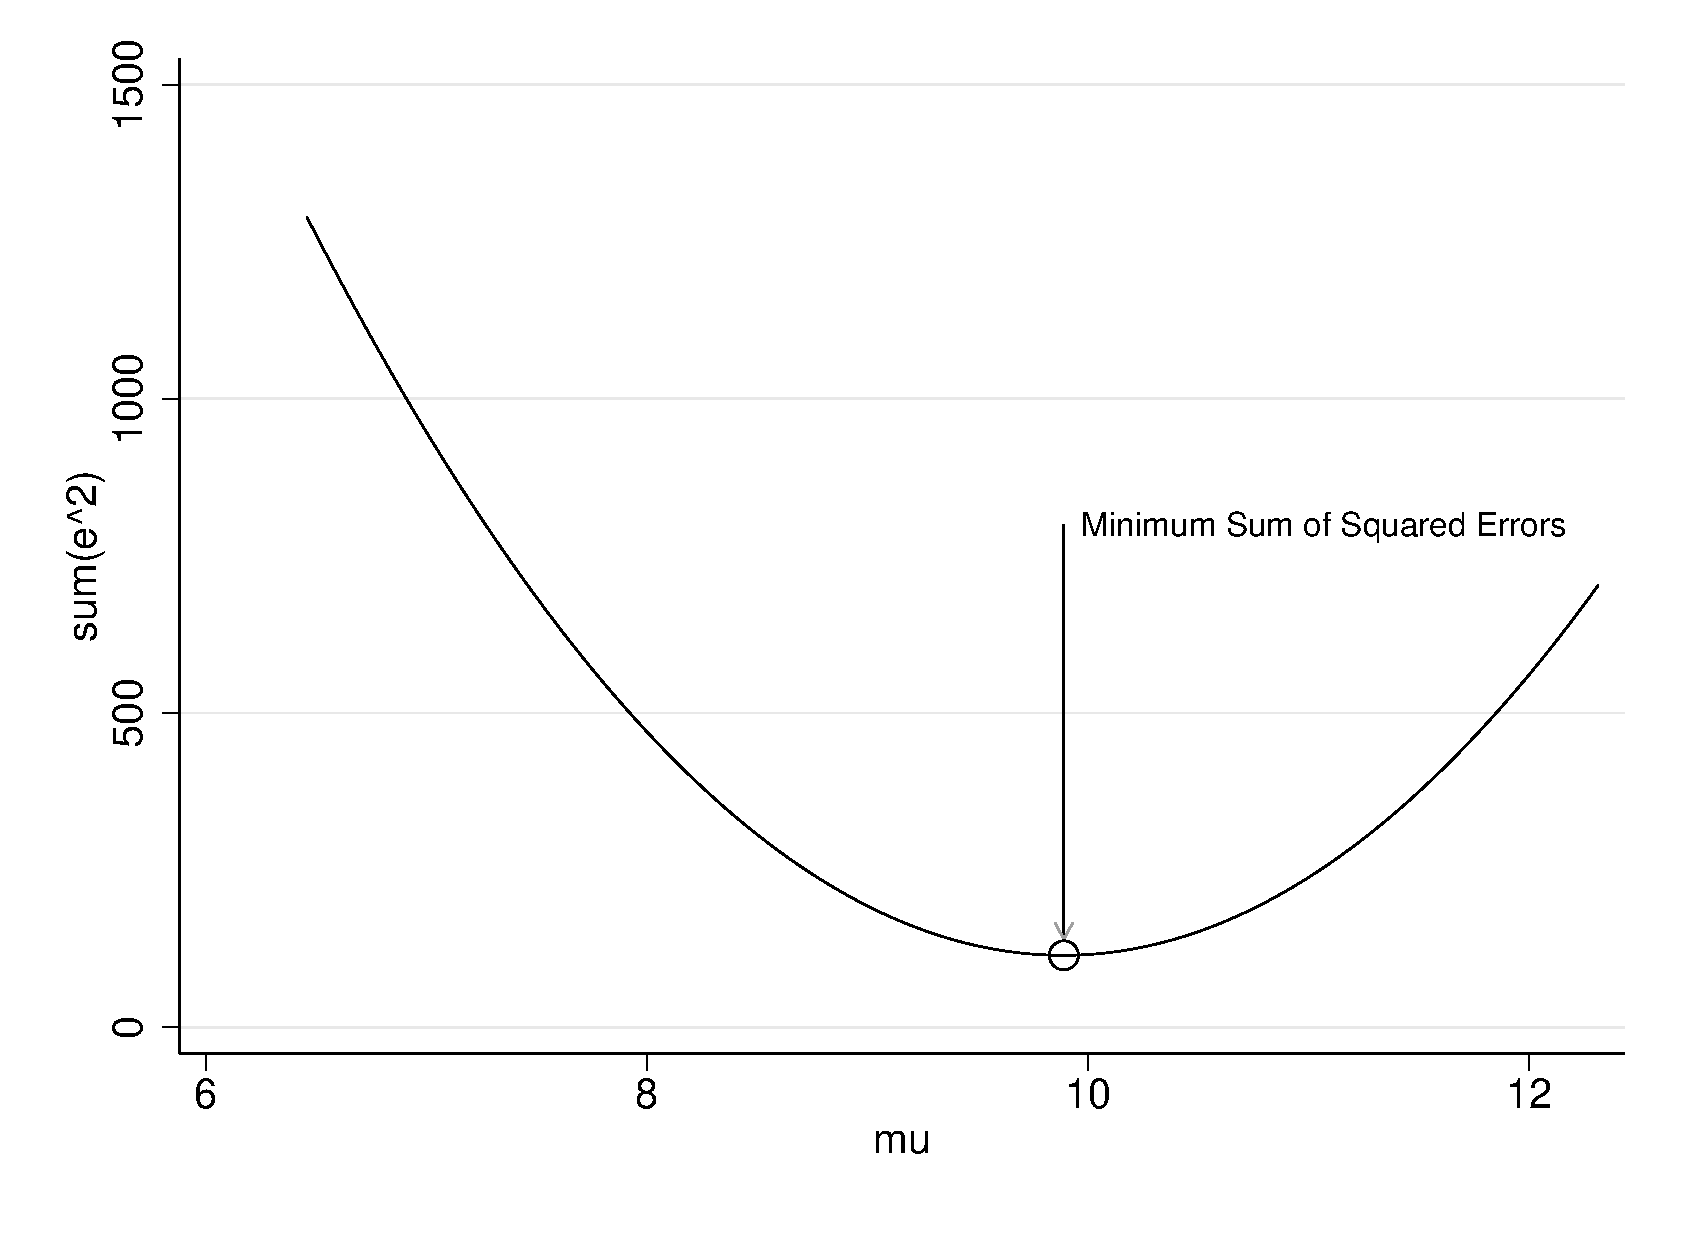
\includegraphics[angle=0,
           width=.75\textwidth]{sse.eps}
   \caption{The SSE as a function of the estimate of the mean for random variable $x$.}
  \label{fig:sse}
\end{figure}

\subsection{Maximum likelihood}
\label{sec:mimean}

Maximum likelihood is a method that expresses the probability of observing a particular parameter, given the observed data. Instead of attempting to minimize the error, this approach attempts to maximize this probability, or likelihood; hence maximum likelihood.

Each time we use maximum likelihood, we much work our parameter estimator assuming a particular distribution. Thus, if our variable is normally distributed we will use a different formula than the one for a binomial variable.

If we are dealing with a normally distributed variable, we can start with the probably of observing the $i^{th}$ value
\begin{equation}
\mbox{Pr}\left(x_i\right)=\frac{1}{\sigma\sqrt{2\pi}}\exp\left[-\frac{1}{2}\sigma^2\left(x_i-\mu\right)^2\right],
\end{equation}
and then the probability of observing a set of $x$s is then
\begin{equation}
\mbox{Pr}\left(x_i\ldots x_N\right)=\prod_{i=1}^N\frac{1}{\sigma\sqrt{2\pi}}\exp\left[-\frac{1}{2}\sigma^2\left(x_i-\mu\right)^2\right],
\end{equation}
or
\begin{equation}
\mbox{Pr}\left(x_i\ldots x_N\right)=\left(\frac{1}{\sigma\sqrt{2\pi}}\right)^N\exp\left[-\frac{1}{2}\sigma^2\sum_{i=1}^N\left(x_i-\mu\right)^2\right],
\end{equation}
we can make the formula easier if we assume that $\sigma= 1$. If we consider the probability of several {\it independent} observations, this likelihood formula becomes a function of the mean
\begin{equation}
\mbox{Pr}\left(\mu\vert x_1\ldots x_N\right)=L\left(\left(\mu\vert x_1\ldots x_N\right)\right)=\left(\frac{1}{\sqrt{2\pi}}\right)^N\exp\left[-\frac{1}{2}\sum_{i=1}^N\left(x_i-\mu\right)^2\right]
\end{equation}
We can take the log of this function to make it more tractable
\begin{equation}
\mbox{ln}\left(L\left(\mu\vert x_1\ldots x_N\right)\right)=-\frac{1}{2}\sum_{i=1}^N\left(x_i-\mu\right)^2-\frac{N}{2}\left(\mbox{ln}\left(\sqrt{2\pi}\right)\right)
\end{equation}
which is something we can handle with basic calculus. We just need to find the derivative of this function with respect to $\mu$. In this situation $\frac{N}{2}\left(\mbox{ln}\left(\sqrt{2\pi}\right)\right)$ is a constant that does not involve $\mu$, and the power rule brings the square (the 2) down as a multiplayer, and $\frac{1}{2}\times 2 = 1$, so the derivative is
\[
\frac{d\mbox{ln}\left(L\left(\mu\vert x_1\ldots x_N\right)\right)}{d\mu}=\sum_{i=1}^N\left(x_i-\mu\right)
\]
take out the sums
\[
\frac{d\mbox{ln}\left(L\left(\mu\vert x_1\ldots x_N\right)\right)}{d\mu}=\sum_{i=1}^Nx_i-N\mu
\]
set to 0 and solve
\[
0=\sum_{i=1}^Nx_i-N\mu
\]
\[
N\mu=\sum_{i=1}^Nx_i
\]
\[
\mu=\frac{\sum_{i=1}^Nx_i}{N}
\]
and there we are, the mean formula again.

\section{The proportion via maximum likelihood}
\label{sec:pml}
While the least squares principle works well for dichotomous variables (the math doesn't care if the numbers only vary between zero and one), the next step is to introduce the idea of likelihood for non-normal distributions. This will be important once we start estimating logits and probits and other models with non-normal distributions. In this section, we figure out the maximum likelihood estimate of a proportion.

Let's start with an example. A researcher takes random poll of 100 people and asks them if they like sardines. Some people said they liked sardines and were coded as 1, while others didn't like sardines and were coded as 0. The frequency table is in Table~\ref{tab:freq_x}.
\begin{table}[htbp]\centering
\caption{Frequency of dichotomous variable $y$\label{tab:freq_x}
\textbf{}}
\begin{tabular} {@{} l r r @{}} \\ \hline
Item& Number & Percent \\
\hline
0=No&    73&    73\\
1=Yes&    27&    27\\
\hline
Total&   100&   100\\
\hline
\multicolumn{3}{@{}l}{\footnotesize{\emph{$\bar{y} = 0.27$}}}
\end{tabular}
\end{table}
The researcher would like to use this data to determine the probability that someone in the population will like sardines, $y$. Of course, we would estimate the mean of this variable to get the proportion.
Why is this the right thing to do? Let's start with the function that determines the chance of observing a "1" or "0" for some variable x, given a probability p
\begin{equation}
f\left(p\vert y\right)=\mbox{Pr}\left(y=q\right)=p^q\left(1-p\right)^{1-q}, q=0,1
\end{equation}
The next important topic is the idea of a likelihood function. Researchers typically want to know the chance of observing the data they have if they assume some pre-specified model. In other words, if our model says that the chance of observing a 1 for any case is 50 percent, then how likely is it that we observed only 27 out of a 100? The likelihood function serves this purpose. It quantifies how likely we are to observe our data if we assume a specific model. In this case, our "model" is just some proportion we expect. Later, our models will become much more complicated multivariate functions. The likelihood function is
\begin{equation}
L\left(p \vert y_1 \ldots y_N\right)=\prod_{i=1}^Nf\left(y_i|p\right)
\end{equation}
To calculate the likelihood function, take the assumed chance of observing (which is $p$ for $y = 1$ and $(1 - p)$ for $y = 0$) for each case and multiply them together. (The symbol $\Pi$ works like the summation symbol, $\Sigma$, except it means multiply everything instead of adding everything). The likelihood function reduces to
\begin{equation}\label{eq:plikelihood}
L\left(p \vert y_1 \ldots y_N\right)=p^{\sum_{i=1}^Ny_i}\left(1-p\right)^{N-\sum_{i=1}^Ny_i}
\end{equation}
Which also looks scarier than it is. It's just the assumed model's probability, $p$, to the power of the total number of observed 1s times $1 - p$ to the power of the total number of observed 0s. Taking the natural log of this function gives us
\begin{equation}
\mbox{ln}\left(L\left(p \vert y_1 \ldots y_N\right)\right)=\left(\sum_{i=1}^Ny_i\right)\mbox{ln}\left(p\right)+\left(N-\sum_{i=1}^Ny_i\right)\mbox{ln}\left(1-p\right)
\end{equation}
Remember from our data that there are 27 yes answers and 100 - 27 = 73 no answers, so thus function is
\[
\mbox{ln}\left(L\left(p \vert y_1 \ldots y_N\right)\right)=\left(27\right)\mbox{ln}\left(p\right)+\left(73\right)\mbox{ln}\left(1-p\right)
\]
\begin{figure}
   \centering
   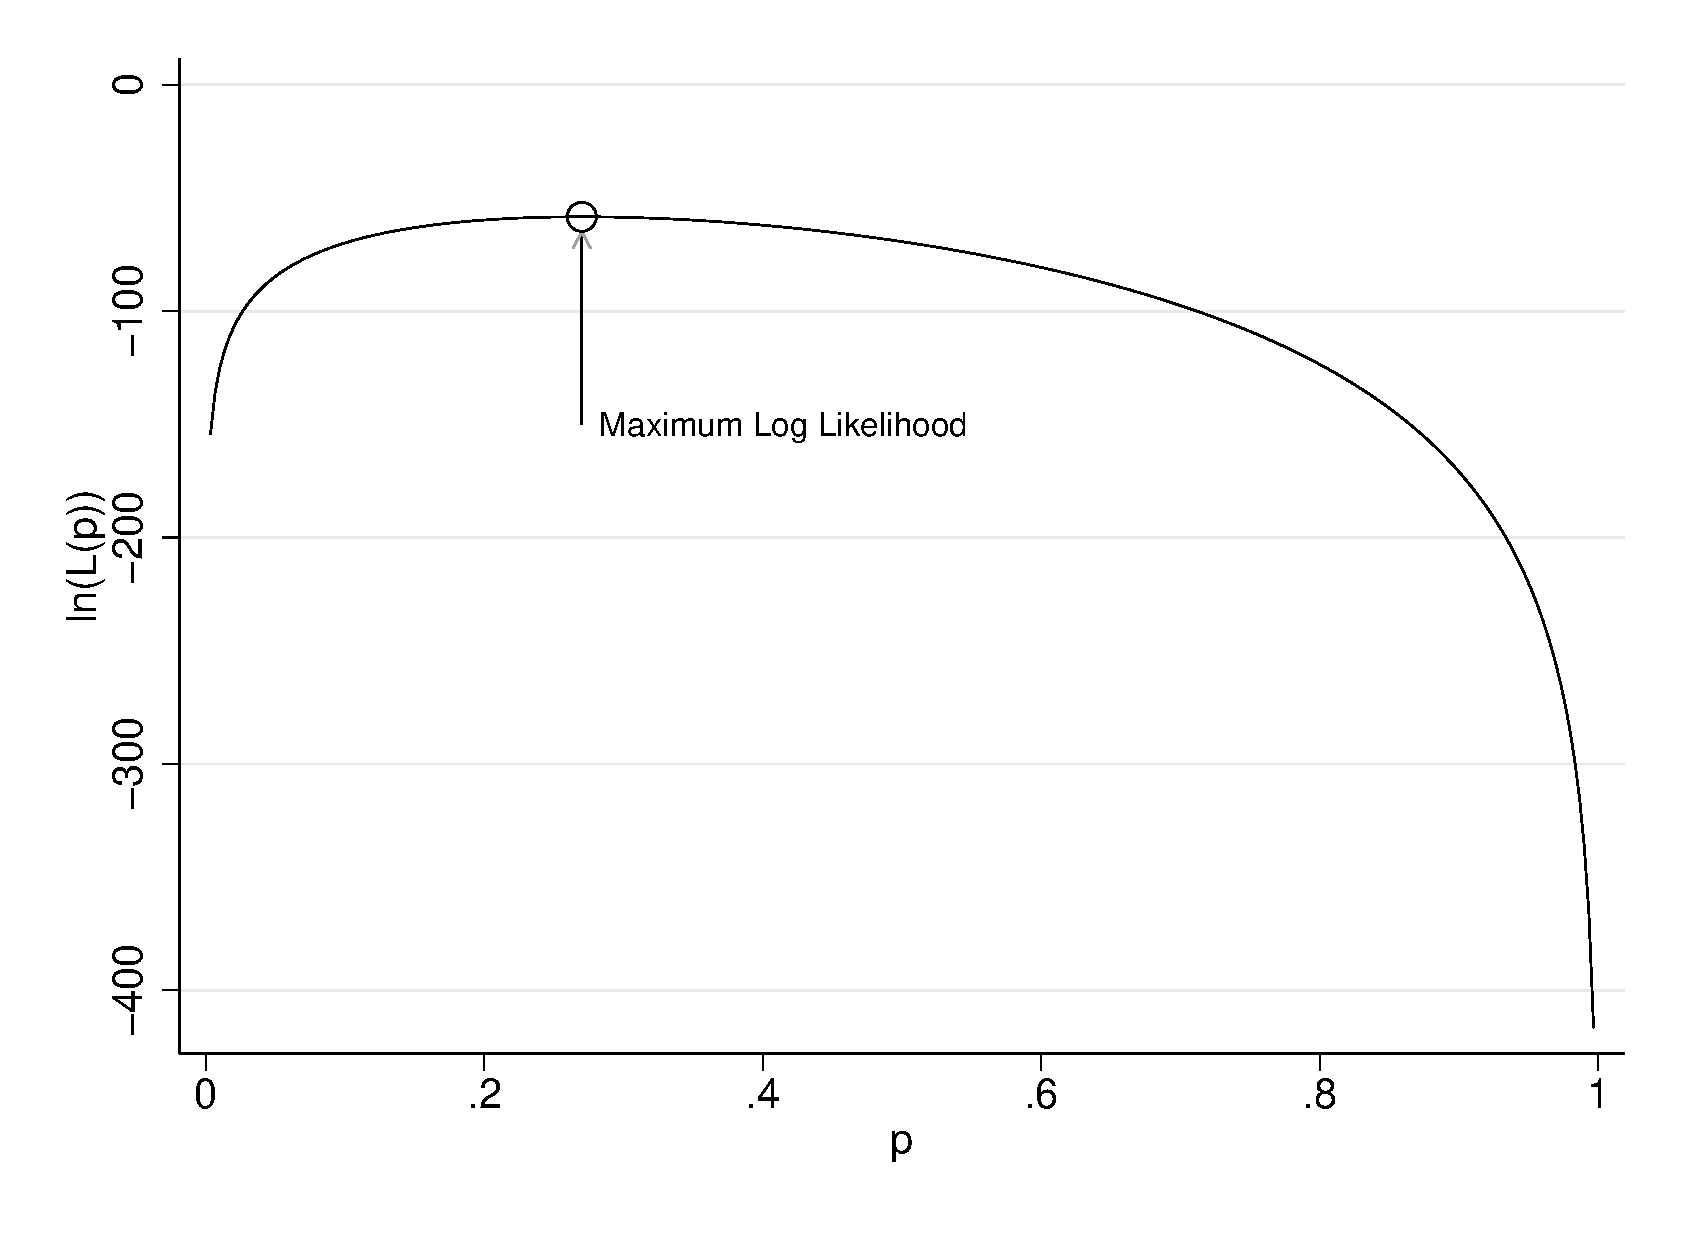
\includegraphics[angle=0,
           width=.75\textwidth]{ll.eps}
   \caption{The likelihood function for random variable $y$ with mean 0.27.}
  \label{fig:ll}
\end{figure}
Figure~\ref{fig:ll} tells a simple story: if one assumes a model where the chance of observing a 1 is the estimated mean, then the likelihood function is maximized. If any other model is assumed, the likelihood function decreases. This suggests that the optimum "model" for our data is the estimated mean. This may seem like we are going in circles, but when we have more complicated models, the idea of maximizing the likelihood of observing the data we have becomes powerful.

What process can be used to find the estimate that maximizes the likelihood? Again, the first step is to find the first derivative (which gives us an equation for slope) of this function with respect to p:
\begin{equation}
\frac{d\mbox{ln}\left(L\left(p \vert y_1 \ldots y_N\right)\right)}{dp}=\frac{\sum_{i=1}^Ny_i}{p}-\frac{N-\sum_{i=1}^Ny_i}{1-p}
\end{equation}
The next step is to set the derivative of this function to 0 (remember, when the slope is 0, the function is either at a local minima or maxima) and solve for p
\[
0=\frac{\sum_{i=1}^Ny_i}{p}-\frac{N-\sum_{i=1}^Ny_i}{1-p}
\]
\[
0=\left(\sum_{i=1}^Ny_i\right)\left(1-p\right)-\left(N-\sum_{i=1}^Ny_i\right)p
\]
\[
-\sum_{i=1}^Ny_i=-pN
\]
\[
-\frac{\sum_{i=1}^Ny_i}{N}=-p
\]
\begin{equation}\label{eq:proportion}
\frac{\sum_{i=1}^Ny_i}{N}=p
\end{equation}

\section*{For more information}
For comprehensive treatment of least squares and maximum likelihood methods, see \citep{eliason1993maximum}. For discussion of likelihood-based inference in regression models, consult \citep{fox} and \citep{gill2006essential}. Additional perspectives on numerical optimization and parameter estimation can be found in \citep{cameron2005microeconometrics}.
There we are, the formula that maximizes the likelihood is the mean, or proportion of 1s. In this case $p = 0.27$. It would be a simple matter to plug in the numbers (if they had been provided) to verify that $p = 0.27$. 



\chapter{Ordinary least squares regression}
\section{A line through the data}
Let's assume that a researcher wants to understand the relationship between two variables, $x$ and $y$, using a geometric line. Recall that a simple two dimensional line has two parameters, and intercept and a slope. In these notes, I call the intercept $\beta_0$ and the slope $\beta_1$ to form the function
\begin{equation}
\hat{y}_i=\beta_0+\beta_1x_i.
\end{equation}
Figure~\ref{fig:fit} is an example line. Note the hat above $y$ again, this lets us know that this is a prediction, not the actual value of $y$. The value of $\hat{y}_i$ is a {\it conditional mean}. If we wanted to show an expression for the actual value of $y$ for each case, we would need to show a residual, $e$, in the expression. This residual is the difference between the actual value of $y$ and the predicted value of $y$:
\begin{figure}
   \centering
   \includegraphics[angle=0,
           width=.75\textwidth]{fit.eps}
   \caption{Data from Table~\ref{tab:xy} fit with $\hat{y}_i=\beta_0+\beta_1x_i$.}
  \label{fig:fit}
\end{figure}
\begin{equation}
e_i=y_i-\hat{y}_i=y_i-\beta_0+\beta_1x_i
\end{equation}
It is also a deviation. Thus, the expression for the observed $y$ that includes the elements of the line is
\begin{equation}
y_i=\beta_0+\beta_1x_i+e_i.
\end{equation}
\begin{figure}
   \centering
   \includegraphics[angle=0,
           width=.75\textwidth]{efit.eps}
   \caption{Data from Table~\ref{tab:xy} fit with $\hat{y}_i=\beta_0+\beta_1x_i$ marked with the value of $e_i$.}
  \label{fig:efit}
\end{figure}
Figure~\ref{fig:efit} shows the residuals for each point on a scatterplot for the simulated data. Note how all the point below the regression line are negative, while all the points above the regression line are positive
\section{The regression slope}
Remember that correlation removes all information about the units of $x$ and $y$. Often, this is not useful to your average policy maker. They generally want to know, "if I put in one more unit of $x$, what happens to $y$?" In other words, if $x$ increases by one unit, what is the change in $y$ (and {\it in the units of $y$}).

We can do this with a regression slope. The formula for the regression slope is quite simple for bivaraite regression, and many parts should look familiar
\begin{equation}\label{eq:olsslope}
\beta_1=\frac{\sum_{i=1}^N\left(y_i-\bar{y}\right)\left(x_i-\bar{x}\right)}{\sum_{i=1}^N\left(x_i-\bar{x}\right)^2}
\end{equation}
Look back at the formula for correlation. This is exactly the same with one change: we removed the sum of squares for $y$ in the denominator. We interpret this statistic as the change in $y$ for a single unit increase in $x$.
\section{The intercept}
In order to draw a line we also need a $y$ intercept. The formula for this is also quite simple, With the slope in hand, we simply calculate the difference between the mean of $y$ and the mean of $x$ times the slope
\begin{equation}\label{eq:olsintercept}
\beta_0=\bar{y}-\beta_1\bar{x}
\end{equation}
This statistic tells us the predicted value of $y$ when $x$ is equal to 0. This will be very important later, as we can change the implicit meaning behind $x = 0$.
\section{Why is this the best fitting line?}
Where did this formula come from? The question to motivate this is: what line best summarizes the data? To answer this question, we need to operationalize what it means to best summarize the data, just as we did for the mean.

\subsection{Least squares formulation}

One idea is that we should first quantify the difference between what we observe for $y$ and what we predict for $y$. The deviation has previously been defined as $e_i$ for each case. Now, how can we summarize these differences in a single number? To do this, we once again return to the sum of squares. We summarize the deviation of the model from the observed as the sum of the squared residuals error ($SSE$)
\begin{equation}
SSE=\sum_{i=1}^Ne_i^2=\sum_{i=1}^N\left(y_i-\hat{y}_i\right)^2
\end{equation}
When $SSE$ is big, the model does a poor job predicting the data. When it's small, the model does a good job predicting the data. Intuitively, this should make sense. The closer the data are to the line, the smaller the $SSE$ will be and the further the data are away from the line, the larger the $SSE$ will be.

Now, how can we find the best line? We have a systematic way of finding the best line to fit the data. Here is the idea: we make $SSE$ a function of the slope and intercept:
\[
S\left(\beta_0,\beta_1\right)=\sum_{i=1}^Ne_i^2
\]
First, we replace the residual with what it is, the difference between $y$ and the regression line
\[
S\left(\beta_0,\beta_1\right)=\sum_{i=1}^N\left(y_i-\beta_0-\beta_1x_i\right)^2
\]
Next, we expand
\[
S\left(\beta_0,\beta_1\right)=\sum_{i=1}^N\left(y_i^2-2\beta_0y_i-2\beta_1y_ix_i+\beta_0^2+2\beta_0\beta_1x_i+\beta_1^2x_i^2\right)
\]
and pull the summations out
\[
S\left(\beta_0,\beta_1\right)=\sum_{i=1}^Ny_i^2-2\beta_0\sum_{i=1}^Ny_i-2\beta_1\sum_{i=1}^Ny_ix_i+N\beta_0^2+2\beta_0\beta_1\sum_{i=1}^Nx_i+\beta_1^2\sum_{i=1}^Nx_i^2
\]
We then find the partial derivative of $\beta_0$ (one of the two normal equations)
\[
\frac{\partial S}{\partial \beta_0}=2N\beta_0-2\sum_{i=1}^Ny_i-2\beta_1\sum_{i=1}^Nx_i
\]
and putting the elements back into the sum
\begin{equation}
\frac{\partial S}{\partial \beta_0}=-2\sum_{i=1}^N\left(y_i-\beta_0-\beta_1x_i\right)
\end{equation}
and the partial derivative of $\beta_1$ (the other normal equation)
\[
\frac{\partial S}{\partial \beta_1}=2\beta_0\sum_{i=1}^Nx_i+2\beta_1\sum_{i=1}^N-2\sum_{i=1}^Ny_ix_i
\]
and putting the elements back into the sum
\begin{equation}
\frac{\partial S}{\partial \beta_1}=-2\sum_{i=1}^N\left(y_i-\beta_0-\beta_1x_i\right)x_i
\end{equation}
We then set these both to 0, pull the constants out, and divide by $N$. That gives us for the intercept
\[
0=\bar{y}-\beta_0-\beta_1\bar{x}
\]
and for the slope
\[
0=\frac{1}{N}\sum_{i=1}^Nx_iy_i-\beta_0\bar{x}-\beta_1\frac{1}{N}\sum_{i=1}^Nx_i^2
\]
Two equations, two unknowns ($\beta_0$ and $\beta_1$). To get $\beta_1$, we figure that $\beta_0$ is
\[
\bar{y}-\beta_0-\beta_1\bar{x}=0
\]
\[
\beta_0=\bar{y}-\beta_1\bar{x}
\]
we then substitute $\bar{y}-\beta_1\bar{x}$ for $\beta_0$ in the second equation
\[
\frac{1}{N}\sum_{i=1}^Nx_iy_i-\beta_0\bar{x}-\beta_1\frac{1}{N}\sum_{i=1}^Nx_i^2 = 0
\]
\[
\frac{1}{N}\sum_{i=1}^Nx_iy_i-\left(\bar{y}-\beta_1\bar{x}\right)\bar{x}-\beta_1\frac{1}{N}\sum_{i=1}^Nx_i^2 = 0
\]
and solve for $\beta_1$
\[
\frac{1}{N}\sum_{i=1}^Nx_iy_i-\bar{y}\bar{x}+\beta_1\bar{x}^2-\beta_1\frac{1}{N}\sum_{i=1}^Nx_i^2 = 0
\]
\[
\frac{1}{N}\sum_{i=1}^Nx_iy_i-\bar{y}\bar{x} = -\beta_1\bar{x}^2+\beta_1\frac{1}{N}\sum_{i=1}^Nx_i^2
\]
\[
\frac{1}{N}\sum_{i=1}^Nx_iy_i-\bar{y}\bar{x} = \beta_1\left(-\bar{x}^2+\frac{1}{N}\sum_{i=1}^Nx_i^2\right)
\]
\[
\frac{\frac{1}{N}\sum_{i=1}^Nx_iy_i-\bar{y}\bar{x}}{\frac{1}{N}\sum_{i=1}^Nx_i^2-\bar{x}^2} = \beta_1
\]
which is the same as equation~\eqref{eq:olsslope}.

The data in Table~\ref{tab:xy} produced the regression in Table~\ref{tab:xyreg}. This is the best fit line. To demonstrate, I attempted to draw some other lines through the data, summed up the residuals, then plotted the $SSE$ for each line against the slope of that line in Figure~\ref{fig:altsse}.

\begin{table}[htbp]\centering
 \caption{Regression of $y$ on $x$ from data in Table~\ref{tab:xy}
\label{tab:xyreg}}
\begin{tabular}{lc}
Coefficients      &    Model  \\
\hline
$x$      &    0.829  \\
      &   (0.384)  \\
Intercept    &    5.032* \\
      &   (1.892)  \\
\hline
\multicolumn{1}{l}{$SE$s in parentheses, $*p<0.05$} \\
\hline
\end{tabular}
\end{table}

\begin{figure}
   \centering
   \includegraphics[angle=0,
           width=.75\textwidth]{altsse.eps}
   \caption{Alternate regression slopes and $SSE$s for data in Table~\ref{tab:xy}; real slope is 0.83.}
  \label{fig:altsse}
\end{figure}
What we find is that no matter what slope I use, I can't do better than the formulas provided here. Compare Figure~\ref{fig:sse} to Figure~\ref{fig:altsse} and you will see how regression works off the same least squares principle.

\subsection{Maximum likelihood formulation}

Another way to get to these estimates is to consider the likelihood of observing the data given the parameters. Since the predicted value $y$ is a conditional mean, we can start with the likelihood function of the mean
\begin{equation}
\mbox{ln}\left(L\left(\mu\vert y_1\ldots y_N\right)\right)=-\frac{1}{2}\sum_{i=1}^N\left(y_i-\mu\right)^2-\frac{N}{2}\left(\mbox{ln}\left(\sqrt{2\pi}\right)\right)
\end{equation}
and replace the mean with the regression formula
\begin{equation}
\mbox{ln}\left(L\left(\beta_0,\beta_1 \vert y_1\ldots y_N\right)\right)=-\frac{1}{2}\sum_{i=1}^N\left(y_i-\beta_0-\beta_1x_i\right)^2-\frac{N}{2}\left(\mbox{ln}\left(\sqrt{2\pi}\right)\right)
\end{equation}
and now we need to find the partial derivatives of this function, which look a lot like the least squares formulations. I won't do that all again, but hopefully you see that taking the derivatives of this function will produce the exact same estimators.  Thus, in this case, the least squares estimators are also the maximum likelihood estimators.

However, the only reason this works is because we assume a normal distribution. That is one of the assumptions of least squares: a normally distributed set of residuals. If that is not the case, then the maximum likelihood estimator will be different altogether, and then the least squares estimators will no longer be valid.



\chapter{Multiple regression}
\label{sec:multiple}

Bivariate regression fits a line to a two-dimensional space. If we have a regression with two predictors we fit a plane to a three-dimensional space. For example,
\begin{equation}
\hat{y}_i=\beta_0+\beta_1x_i+\beta_2z_i
\end{equation}
is an equation for plane and provides a formula for points on a (y,x,z) coordinate system. By fitting a plane to the data, regression can independently estimate the effects of one variable, while holding the other constant. The best way to think about multiple regression is with matrix algebra

\section{The matrix algebra formulation}
Thus, one of the beauties of regression is that we can have more than one predictor. Using two variables for example, we could fit a plane to the variables $x_1$ and $x_2$:
\begin{equation}
\hat{y}_i=\beta_0+\beta_1x_{1i}+\beta_2x_{2i}
\end{equation}
We could fit a hyperplane to three predictors, indexed as $x_1$, $x_2$, and $x_3$:
\begin{equation}
\hat{y}_i=\beta_0+\beta_1x_{1i}+\beta_2x_{2i}+\beta_3x_{3i}
\end{equation}
and so on.
The problem is the algebra for these solutions gets complicated fast. Instead, we have a matrix algebra equivalent of our least squares estimator
\begin{equation}\label{eq:olsmatrix}
{\bf{b=\left(X'X\right)^{-1}X'y}}
\end{equation}
\begin{table}[htbp]\centering
\caption{Small set of 4 cases\label{tab:mxy}
\textbf{} }\begin{tabular} {@{} l r @{}} \\
$y$ & $x$ \\
\hline
3 &4\\
2 &3\\
4 &3\\
5 &6\\
\hline
\multicolumn{2}{@{}l}{\footnotesize{\emph{} }}
\end{tabular}
\end{table}

Matrix algebra is powerful. It deals with vectors (single rows or columns of data) and matrixes (data with multiple rows and columns). Statistics packages take the data in tables and convert them to matrixes. For instance, we can think of our outcome in Table~\ref{tab:mxy} as a vector of numbers called ${\bf{y}}$, for example:
\[
{\bf{y}}=
\begin{bmatrix}
3 \\
2 \\
4 \\
5 \\
\end{bmatrix}
\]
Here we have 4 cases ($N$ = 4) where the first case of $y$ is 3, the second case of $y$ is 2, the third case of $y$ is 4, and the fourth case of $y$ is 5. We can then think of our predictors as a matrix with $N$ rows and $p$ columns
\[
{\bf{X}}=
\begin{bmatrix}
1&4 \\
1&3 \\
1&3 \\
1&6 \\
\end{bmatrix}
\]
The first column is for the intercept. That's why some programs call it a constant, because it is for a "variable" that is a constant value of 1s. Thus, we can then think of our typical regression equation as
\begin{equation}\label{eq:matrixolsmodel}
{\bf{y=Xb+e}}
\end{equation}
\[
\begin{bmatrix}
y_i \\
\vdots \\
y_N \\
\end{bmatrix}
= \\
\begin{bmatrix}
1&x_{11}&\cdots&x_{p11} \\
\vdots&\vdots&\ddots&\vdots \\
1&x_{1N}&\cdots&x_{pN} \\
\end{bmatrix}
\begin{bmatrix}
\beta_0 \\
\beta_1 \\
\vdots \\
\beta_p \\
\end{bmatrix}
+ \\
\begin{bmatrix}
e_1 \\
\vdots \\
e_N \\
\end{bmatrix}
\]
Note how easy it is to formulate any number of predictors, the regression equation always comes out to ${\bf{y=Xb+e}}$. Now, the formula to obtain the slopes (or the b vector) is
\[
{\bf{b=\left(X'X\right)^{-1}X'y}}
\]
This may not look familiar, but it is. For instance,
\[
{\bf{\left(X'X\right)}}=\sum_{i=1}^N\left(x_i-\bar{x}\right)^2
\]
which is the denominator of the slope formula, and since
\[
a^{-1} = \frac{1}{a}
\]
Also,
\[
{\bf{X'y}} =\sum_{i=1}^N\left(y_i-\bar{y}\right)\left(x_i-\bar{x}\right)
\]
which is the numerator of the slope formula.

Matrix algebra has many rules, and I'm not going to go through all of them here. However, here is an example calculation with the small set of 4 in Table~\ref{tab:mxy}. First, we need to transpose ${\bf X}$ to get ${\bf X'}$ (also known as ${\bf X}$ prime or the transpose of ${\bf X}$):
\[
{\bf X'} =
\begin{bmatrix}
1&1&1&1 \\
4&3&3&6 \\
\end{bmatrix}
\]
Note that the transpose of ${\bf X}$ simply makes rows out of columns. Column 1 becomes row 1, column 2 becomes row 2, and so on. ${\bf X'X}$ is multiplying ${\bf X'}$ and ${\bf X}$ (note: in matrix algebra the order of multiplication matter a lot). So, if
\[
{\bf X'} =
\begin{bmatrix}
a_{11}&a_{12}&a_{13}&a_{14} \\
a_{21}&a_{22}&a_{23}&a_{24} \\
\end{bmatrix}
\]
and
\[
{\bf X} =
\begin{bmatrix}
b_{11} & b_{12} \\
b_{21} & b_{22} \\
b_{31} & b_{32} \\
b_{41} & b_{42} \\
\end{bmatrix}
\]
then
\begin{equation}
{\bf X'X} =
\begin{bmatrix}
\left(\sum_ia_{1i}b_{i1}\right)&\left(\sum_ia_{1i}b_{i2}\right) \\
\left(\sum_ia_{2i}b_{i1}\right)&\left(\sum_ia_{2i}b_{i2}\right) \\
\end{bmatrix}
\end{equation}
This means that we can compute X'X like so
\[
\sum_ia_{1i}b_{i1} = \left(\left(1\times1\right)+(\left(1\times1\right)+(\left(1\times1\right)+(\left(1\times1\right)\right)
\]
\[
\sum_ia_{1i}b_{i2} = \left(\left(4\times1\right)+(\left(3\times1\right)+(\left(3\times1\right)+(\left(6\times1\right)\right)
\]
\[
\sum_ia_{2i}b_{i1} = \left(\left(1\times4\right)+(\left(1\times3\right)+(\left(1\times3\right)+(\left(1\times6\right)\right)
\]
\[
\sum_ia_{2i}b_{i2} = \left(\left(4\times4\right)+(\left(3\times3\right)+(\left(3\times3\right)+(\left(6\times6\right)\right)
\]
which means
\[
{\bf X'X} =
\begin{bmatrix}
4&16 \\
16&70 \\
\end{bmatrix}
\]
Next, we tackle ${\bf X'y}$. If
\[
{\bf y} =
\begin{bmatrix}
b_{11} \\
b_{12} \\
b_{13} \\
b_{14} \\
\end{bmatrix}
\]
then
\begin{equation}
{\bf X'y} =
\begin{bmatrix}
\left(\sum_ia_{1i}b_{i1}\right) \\
\left(\sum_ia_{2i}b_{i1}\right) \\
\end{bmatrix}
\end{equation}
which translates into
\[
\sum_ia_{1i}b_{i1} = \left(1\times3\right)+\left(1\times2\right)+\left(1\times4\right)+\left(1\times5\right)
\]
\[
\sum_ia_{2i}b_{i1} = \left(4\times3\right)+\left(3\times2\right)+\left(3\times4\right)+\left(6\times5\right)
\]
\[
{\bf X'y} =
\begin{bmatrix}
14 \\
16 \\
\end{bmatrix}
\]
Now, we need to invert $\bf X'X$. So, if
\[
{\bf X'X} =
\begin{bmatrix}
a&b \\
c&d \\
\end{bmatrix}
\]
and
\begin{equation}
\left({\bf X'X}\right)^{-1} =
\begin{bmatrix}
\left(\frac{d}{ad-bc}\right)&\left(\frac{-b}{ad-bc}\right) \\
\left(\frac{-c}{ad-bc}\right)&\left(\frac{a}{ad-bc}\right) \\
\end{bmatrix}
\end{equation}
and also if
\[
ad-bc = 24
\]
then
\[
\left({\bf X'X}\right)^{-1} =
\begin{bmatrix}
2.92&-0.67 \\
-0.67&0.16 \\
\end{bmatrix}
\]
Bring it all together:
\[
{\bf b = \left(X'X\right)^{-1}X'y} =
\begin{bmatrix}
\left(\sum_ia_{1i}b_{i1}\right) \\
\left(\sum_ia_{2i}b_{i1}\right) \\
\end{bmatrix}
\]
Which means we are left with
\[
\bf b =
\begin{bmatrix}
0.83 \\
0.66 \\
\end{bmatrix}
\]
where 0.83 is our intercept, $\beta_0$, and 0.66 is our slope $\beta_1$. There we are. It is not important that you be able to do this, but I do want you to remember the formula $\bf b = \left(X'X\right)^{-1}X'y$ because we are going to alter it from time to time for different estimators.

\subsection{The matrix formulation of least squares}

We can still show that these are least squares estimates. In matrix form, the sum of squares is $\bf e'e$, so we can write the matrix of slopes as a function of the sum of squares
\[
S\left({\bf b}\right)={\bf e'e}
\]
\[
S\left({\bf b}\right)={\bf \left(y-Xb\right)'\left(y-Xb\right)}
\]
\begin{equation}
S\left({\bf b}\right)={\bf y'y-\left(2y'X\right)b+b'\left(X'X'\right)b}
\end{equation}
We then again find the derivative
\begin{equation}
\frac{\partial S\left({\bf b}\right)}{\partial {\bf b}}={\bf 2X'Xb-2X'y}
\end{equation}
set the derivative to 0 and solve
\[
0={\bf 2X'Xb-2X'y}
\]
\[
{\bf -2X'Xb}={\bf -2X'y}
\]
\[
{\bf X'Xb}={\bf X'y}
\]
\[
{\bf b}={\bf \left(X'X\right)^{-1}X'y}
\]
the result matches equation~\eqref{eq:olsmatrix}.

\subsection{The matrix formulation of maximum likelihood}
\label{sec:regml}

We can also get to this estimate through maximum likelihood. If the mean is equal to the slopes and predictors combination, $\bf Xb$, then the likelihood of observing our data from our parameters is
\begin{equation}
\mbox{ln}\left(L\left({\bf b, V \vert \bf y}\right)\right)=-\frac{N}{2}\mbox{ln}\left(2\pi\right)-\frac{N}{2}\mbox{ln}\left(\bf V\right)-\frac{1}{2}{\bf \left(y-Xb\right))'V^{-1}\left(y-Xb\right)}
\end{equation}
 where $\bf V$ is the variance-covariance matrix of residuals. After some work, we can find the partial derivative of this function with respect to the slopes, $\bf b$ as
\begin{equation}
\frac{\partial\mbox{ln}\left(L\left({\bf b, V \vert \bf y}\right)\right)}{\partial \bf b} = {\bf -X'V^{-1}Xb+X'V^{-1}y}
\end{equation}
we then set to 0 and solve
\[
0= {\bf -X'V^{-1}Xb+X'V^{-1}y}
\]
\[
{\bf X'V^{-1}Xb}= {\bf X'V^{-1}y}
\]
\[
{\bf b}= {\bf \left(X'V^{-1}X\right)^{-1}X'V^{-1}y}
\]
As we see in Chapter~\ref{sec:het}, a very important set of assumptions in OLS regression is that the errors have 0 correlation and constant variance. this allows $\bf V$ to be a simple matrix where the diagonals are all $\sigma^2$ and every other number in the matrix is 0. Thus, $\bf V$ drops out and we are left with equation~\eqref{eq:olsmatrix},
\[
{\bf b}={\bf \left(X'X\right)^{-1}X'y}
\]
 The OLS estimator.

\section{Interpretation}
The general regression model is expressed algebracially like this
\begin{equation}
\hat{y}_i=\beta_0+\sum_p\beta_px_{ip}
\end{equation}
where $\sum_p\beta_px_{ip}$ is my shorthand for each $p$ predictor and its associated slope. We interpret the intercept, $\beta_0$, as the predicted value of $y$ when all predictors are equal to 0. Later we will do many neat things to control what the intercept means substantively by messing with what $x_p$ means.

Each slope for any predictor is then interpreted as the change in the predicted value of $y$, in the units of $y$ if we increase by one unit. Again, we can control what means substantively, and we will go over that later.


\section{Standardized coefficients}
One question that is often important to researchers is whether one variable is more important than another in predicting the outcome.

We can do this with the standardized regression coefficient. This is a scaled slope that takes into account the ratio of the standard deviation of the predictor to the standard deviation of the outcome
\begin{equation}
\beta_p^*=\beta_p\frac{s_p}{s_y}
\end{equation}
This procedure makes comparisons between predictors possible because its interpretation is changed from the change in $y$ for a one unit increase in $x$ (in the units of $x$) to the {\it standard deviation unit} change in $y$ for a {\it standard deviation increase} in $x$.

Be careful in doing this with dichotomous predictors.

\subsection{Standardized coefficient example}
Table~\ref{tab:wagesum} details the summary statistics for 200 observations from a dataset that collections wage, education, age and gender.

\begin{table}[htbp]
\caption{\label{tab:wagesum} Summary Statistics for Wage Model}\centering\medskip
\begin{tabular}{lcccc}
 & mean & sd & min & max \\ \hline
wage & 16.03 & 8.32 & 3.13 & 45.36 \\
edu & 13.48 & 2.91 & 5 & 20 \\
age & 36.73 & 12.31 & 16 & 64 \\ \hline
 \end{tabular}
\end{table}
\begin{table}[htbp]\centering
 \caption{Model predicting wages by education and age
\label{tab:wagereg}}
\begin{tabular}{lc}
\hline
Coefficients      &    Model  \\
\hline
edu     &    0.882***\\
      &   (0.184)  \\
age     &    0.218***\\
      &   (0.043)  \\
Intercept    &   -3.866  \\
      &   (3.061)  \\
\hline
\multicolumn{1}{l}{Model Statistics} \\
\hline
$N$      &   200.000  \\
$F$      &   22.947  \\
$R^2$     &    0.189  \\
$df$ Regression     &    2.000  \\
Sum of Squares Regression     &  2603.472  \\
$df$ Error    &   197.000 \\
Sum of Squares Error    &  11175.277  \\
\hline
\multicolumn{1}{l}{$SE$s in parentheses, $***p<0.001$} \\
\hline
\end{tabular}
\end{table}
Table~\ref{tab:wagereg} presents the regression model for wages as a function of education (edu) and age.
We can calculate the standardized coefficients using the information in Tables~\ref{tab:wagesum} and~\ref{tab:wagereg}. For example, the standardized coefficient for edu is
\[
\beta_{edu}^*=\beta_{edu}\frac{s_{edu}}{s_{wage}}=0.882\frac{2.91}{8.32}=0.308
\]
and for age is
\[
\beta_{age}^*=\beta_{age}\frac{s_{age}}{s_{wage}}=0.218\frac{12.31}{8.32}=0.322
\]
You will notice that even though the coefficient for education was larger, the standardized coefficient for age was larger because age had a larger standard deviation.
\section{Introduction to coding and interpreting nominal predictors}
So far we have only worked with regression predictors that are continuous in nature. However, in social science we often have nominal variables of interest that we think would make good predictors of continuous outcomes (for nominal outcomes, see the logit and probit chapter). This is just a brief introduction, we will have a chapter devoted to other things you can do with nominal variables.
\subsection{Two groups}
We can consider a variable dichotomous when it takes on only two values, 0 and 1. This can indicate a trait of some sort, or may simply be a way to organize a variable with two values.

In the bivariate case, the slope, standard error, and $t$-test of some outcome $y$ regressed on a dichotomous predictor $d$ will give the same answer as the independent groups' $t$-test. That is to say that in the model
\begin{equation}
y_i=\beta_0+\beta_1d_i+e_i
\end{equation}
the value of $\beta_1$ equals the difference between the average of $y$ when $d=1$ and $d=0$
\begin{equation}
\beta_1 = \left(\bar{y}|d=1\right)-\left(\bar{y}|d=0\right)
\end{equation}
Also, the standard error of $\beta_1$ is the same standard error from the independent test. As a result, the $t$-test and result are also the same.
\subsection{More than two groups}

We could use ANOVA to test generally whether these means are different. Table~\ref{tab:wordanova} told us with an $F$ test of 16.87, and with (2,2588) degrees of freedom, that groups were different.  Unfortunately, this doesn't tell us about who is different, just that at least one group is.

What we need is to enter dichotomous (or "dummy") variables into a regression model. This works by creating for each category in $x$ (except one reference group) new variables, $d_j$ where $j\in\left\{1 \ldots k\right\}$ that is equal to 1 if that case is a member of that group, and 0 otherwise:
\begin{equation}
d_j = \left\{ \begin{array}{ll}
     1 & \mbox{if $x = j$};\\
     0 & \mbox{otherwise}.\end{array} \right.
\end{equation}
Picking moderate as our reference group, and creating variables $lib$ and $con$, we can fit the following model
\[
\widehat{words}_i=\beta_0+\beta_1lib_i+\beta_2con_i
\]
This model is presented in Table~\ref{tab:wordmodel}. Note that the $F$-test is the same as what was reported by the ANOVA model.
\begin{table}[htbp]\centering
 \caption{Model predicting words correct by political affiliation
\label{tab:wordmodel}}
\begin{tabular}{lc}
\hline
Coefficients      &    Model  \\ \hline
lib &    0.513***\\
      &   (0.097)  \\
con &    0.422***\\
      &   (0.093)  \\
Intercept    &    5.812***\\
      &   (0.064)  \\
\hline
\multicolumn{1}{l}{Model Statistics} \\
\hline
$N$          &   2591.000  \\
$F$          &   16.869  \\
$R^2$        &    0.013  \\
$df$ Regression      &    2.000  \\
Sum of Squares Regression     &  134.432  \\
$df$ Error    &   2588.000  \\
Sum of Squares Error    &  10311.878  \\
\hline
\multicolumn{1}{l}{$SE$s in parentheses, $***p<0.001$} \\
\hline
\end{tabular}
\end{table}
A few things to note in this model. First, the intercept is the predicted value of $y$ when all predictors are equal to 0. Thus, this is the predicted value for the reference group (moderate).

Compare the constant with the mean of the moderate group. It's the same. Now, also compare the effect of $lib$, it is the difference in the means of the liberal group and the moderates. The effect of $con$ is the difference in the means of the conservative group and the moderates.

Sometimes researchers do not want to know the difference between a particular group and a reference group. Perhaps the research question is about the difference between a particular group and the population average, or specifically the average of group averages. In this case we use deviance coding. In deviance coding, instead of just a simple "1 for the group and 0 otherwise," we instead code each group as 1 for the group, -1 for the reference ($m$), and 0 otherwise:
\begin{equation}
d_j = \left\{ \begin{array}{ll}
     1 & \mbox{if $x = j$};\\
     -1 & \mbox{if $x = m$};\\
     0 & \mbox{otherwise}.\end{array} \right.
\end{equation}
we then fit the model with this coding
\begin{table}[htbp]\centering
 \caption{Model predicting words correct by political affiliation--deviance coding
\label{tab:wordreg_dc}}
\begin{tabular}{lc}
\hline
Coefficients      &    Model  \\ \hline
lib     &    0.201***\\
      &   (0.058)  \\
con     &    0.111* \\
      &   (0.055)  \\
Intercept    &    6.124***\\
      &   (0.040)  \\
\hline
\multicolumn{1}{l}{Model Statistics} \\
\hline
$N$          &   2591.000  \\
$F$          &   16.869  \\
$R^2$        &    0.013  \\
$df$ Regression      &    2.000  \\
Sum of Squares Regression     &  134.432  \\
$df$ Error    &   2588.000  \\
Sum of Squares Error    &  10311.878  \\
\hline
\multicolumn{1}{l}{$SE$s in parentheses, $***p<0.001$} \\
\hline
\end{tabular}
\end{table}
Now the intercept is an estimate of the average of group averages $((6.32 + 5.81 + 6.23)/3) = 6.12$, and each slope is the difference between that group and the average of group averages. For example, we see a difference of 0.20 words between liberals and and the average of group averages. Note, also, that all the model statistics are the same.

\begin{table}[htbp]\centering
 \caption{Model predicting words correct by political affiliation--linear contrasts
\label{tab:wordreg_contr}}
\begin{tabular}{lc}
\hline
Coefficients      &    Model  \\ \hline
$constrast_1$     &   -0.312***\\
      &   (0.054)  \\
$constrast_2$     &    0.045  \\
      &   (0.050)  \\
Intercept    &    6.124***\\
      &   (0.040)  \\
\hline
\multicolumn{1}{l}{Model Statistics} \\
\hline
$N$          &   2591.000  \\
$F$          &   16.869  \\
$R^2$        &    0.013  \\
$df$ Regression      &    2.000  \\
Sum of Squares Regression     &  134.432  \\
$df$ Error    &   2588.000  \\
Sum of Squares Error    &  10311.878  \\
\hline
\multicolumn{1}{l}{$SE$s in parentheses, $***p<0.001$} \\
\hline
\end{tabular}
\end{table}


A third method of coding variables is linear contrasts. Suppose, after our investigation, that we wanted to test other hypotheses such as how two groups compared to another. Suppose we wanted to test the null hypotheses that moderates were less smart than the average of liberals and conservatives. Such a hypothesis would be
\[
H_0:\mu_{mod}=\frac{\mu_{lib}+\mu_{con}}{2}
\]
which can be rewritten as
\[
H_0:0=1\times\mu_{mod}-0.5\times\mu_{lib}-0.5\times\mu_{con}
\]
A second hypothesis would test specifically whether liberals could be smarter than conservatives, ignoring moderates.
\[
H_0:\mu_{lib}=\mu_{con}
\]
which can be rewritten as
\[
H_0:0=0\times\mu_{mod}+1\times\mu_{lib}-1\times\mu_{con}
\]
and all could be symbolized generally with contrast coefficients
\[
H_0:0=c_1\times\mu_{mod}+c_2\times\mu_{lib}+c_3\times\mu_{con}
\]
where $c_1$, $c_2$, and $c_3$, are the contrast coefficients. We create new variables for each set of contrast coefficients. For example, we create a new variable $contrast_1$ that is equal to 1 ($c_1$) for moderates, -0.5 for both liberals ($c_2$) and conservatives ($c_3$). We then create another variable, $contrast_2$ that is equal to 0 ($c_1$) for moderates, 1 for liberals ($c_2$), and \[
\widehat{words}_i=\beta_0+\beta_1contrast_1+\beta_2contrast_2
\]
The results of this model are in Table~\ref{tab:wordreg_contr}. The effect of the first contrast shows that the moderate average is less than the average of liberals and conservatives. We see that the first contrast is statistically signifiant. However, the second contrast is not: liberals are not smarter than conservatives. Again, the model fit statistics are the same. For any set of contrasts, there are three sets of rules:
\begin{enumerate}
 \item The coefficients must add to 0 for each contrast
 \item The sum of the products of all contrasts must equal 0
 \item You must have $m$-1 contrasts, where $m$ is the number of categories
\end{enumerate}

\chapter{OLS model inference and evaluation}\citep{fox}
So now we know how to get slopes and the intercept. Now we need to get a handle on whether we can conclude anything substantive about them. There are two aspects to model evaluation: hypothesis tests of coefficients and evaluating model fit. These topics are of course connected and we see that when we test blocks of coefficients.

Let us consider, again, a model where wages are a function of education and other variables. In Tables~\ref{tab:wagesum} and~\ref{tab:wagereg} I referenced a dataset of 200 observations with three variables: hourly wages ("wage"), years of education ("edu"), and age. Table~\ref{tab:wagereg_all} displays three different models. The first model is simply
\begin{equation}
\hat{y}_i=\beta_0+\beta_1edu_i
\end{equation}
the second model adds age to the model
\begin{equation}
\hat{y}_i=\beta_0+\beta_1edu_i+\beta_2age_i
\end{equation}
and the final model adds a dichotomous female indicator
\begin{equation}
\hat{y}_i=\beta_0+\beta_1edu_i+\beta_2age_i+\beta_3female_i
\end{equation}
\begin{table}[htbp]\centering
 \caption{Models predicting wages
\label{tab:wagereg_all}}
\begin{tabular}{lccc}
\hline
Coefficients  &   Model 1  &   Model 2  &   Model 3  \\ \hline
edu     &    0.835***&    0.882***&    0.847***\\
      &   (0.195)  &   (0.184)  &   (0.184)  \\
age     &        &    0.218***&    0.229***\\
      &        &   (0.043)  &   (0.044)  \\
female   &        &        &   -2.033  \\
      &        &        &   (1.074)  \\
intercept  &    4.780  &   -3.866  &   -2.817  \\
      &   (2.682)  &   (3.061)  &   (3.091)  \\
\hline
\multicolumn{4}{l}{Model Statistics} \\
\hline
$N$   &   200.000  &   200.000  &   200.000  \\
$F$    &   18.410  &   22.947  &   16.692  \\
$R^2$   &    0.085  &    0.189  &    0.204  \\
$df$ Regression    &    1.000  &    2.000  &    3.000  \\
Sum of Squares Regression  &  1172.179  &  2603.472  &  2804.011  \\
$df$ Error    &   198.000  &   197.000  &   196.000  \\
Sum of Squares Error   &  12606.570  &  11175.277  &  10974.738  \\
\hline
\multicolumn{4}{l}{$SE$s in parentheses, $***p<0.001$} \\
\hline
\end{tabular}
\end{table}
Table~\ref{tab:wagereg_all} gives a lot information. First we get the slopes and intercept on the upper table. Second, we get model fit statistics on the lower table. In this section, I describe these measures.
\section{The variance and covariance of regression coefficients}
\label{sec:matrixv}
In statistics, we are obsessed with the variance of our estimators. The variance of an estimator is just the square of the standard error. Thus, once we know the variance of the estimator, we can just get the square root and use that for hypothesis testing. In matrix notation, the variance of the regression slopes is
\begin{equation}
\bf V\left({\hat{b}}\right)=\left(\frac{1}{N}X'X\right)^{-1}\sigma^2
\end{equation}
where $\sigma^2$ is the variance of the regression residuals, or
\begin{equation}
\sigma^2 = \frac{\sum_{i=1}^N\left(e_i-\bar{e}\right)^2}{N-p}
\end{equation}
and $\bf X'X$ is the sum of squares of the matrix of predictors. We can express this with conventional algebra in the bivariate regression model as
\begin{equation}\label{eq:olsb1var}
\mbox{var}\left(\beta_1\right)=\frac{\sigma^2}{\sum_{i=1}^N\left(x_i-\bar{x}\right)^2}
\end{equation}
and we can express the standard error of the slope as the square root of this
\begin{equation}
SE\left(\beta_1\right)=\sqrt{\frac{\sigma^2}{\sum_{i=1}^N\left(x_i-\bar{x}\right)^2}}
\end{equation}
Here we see that the variance, and thus the standard error, is a function of the variance in the residuals and the variance in the predictor. It's the variance in the predictor that is the big player here. The larger the variance in $x$, or the more $x$ is "spread out," the smaller the standard error.
This is related to this is the variance of predicted point, $\hat{y}_0$, where again the crucial ingredient is the variance of $x$
\begin{equation}\label{eq:varfit}
\mbox{var}\left(\hat{y}_0\right)=\left(\frac{\sigma^2}{N}+\frac{\left(x_0-\bar{x}\right)^2\sigma^2}{\sum_{i=1}^N\left(x_i-\bar{x}\right)^2}\right)\sigma^2
\end{equation}
Here, $\hat{y}_0$ is the predicted value of $y$ associated with a hypothetical value of $x$, $x_0$. We see that as the hypothetical value of $x$ moves away from the mean of $x$, that the variance will increase.  This formula allows us to construct a confidence interval for each prediction
\begin{equation}
CI\left(\hat{y}_0,\left(1-\alpha\right)\times100\right)=\hat{y}_0\pm t_{df,\alpha/2}\sqrt{\left(\frac{\sigma^2}{N}+\frac{\left(x_0-\bar{x}\right)^2\sigma^2}{\sum_{i=1}^N\left(x_i-\bar{x}\right)^2}\right)\sigma^2}
\end{equation}
Thus, the greater the variance in $x$, the smaller the confidence interval in any predicted value of $y$. A smaller confidence interval means that the range of possible slopes for $y$ is smaller.
\begin{figure}
   \centering
   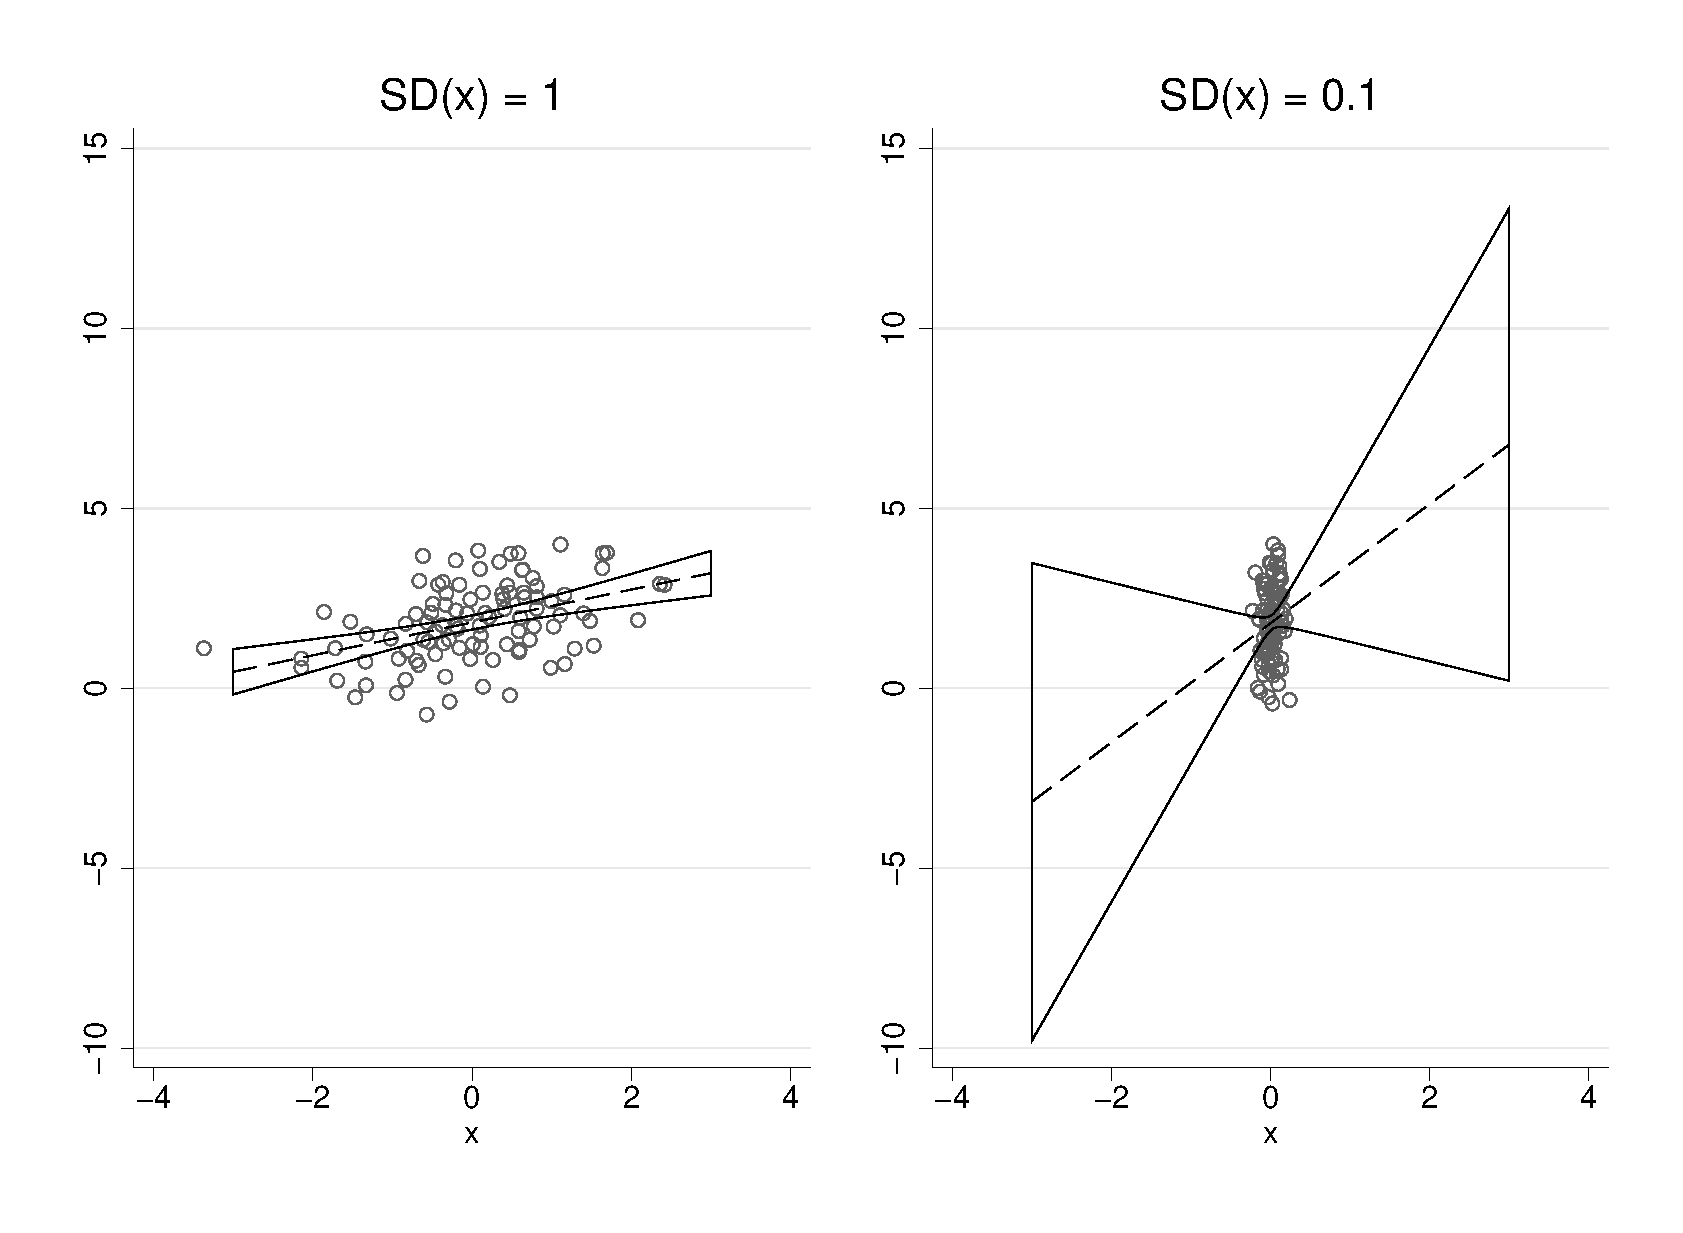
\includegraphics[angle=0,
           width=.75\textwidth]{cislope.eps}
   \caption{Variance of regression slopes as a function of the variance of $x$}
  \label{fig:cislopes}
\end{figure}
Figure~\ref{fig:cislopes} features this difference. The panel on the left is a situation in which $x$ has the larger standard deviation. We see that the slope is accurate and the 95 percent confidence interval (the fan like shape around the prediction line) of the prediction is pretty tight, implying a small standard error of the slope. The panel on the right, however, $x$ has a small standard deviation and we see that the range of possible slopes is large because the 95 percent confidence interval of values is quite high.
\section{Hypothesis testing with regression slopes}
Recall our hypothesis testing for the difference between means. We were testing the difference between two mean values of $y$, $\bar{y}_A$ and $\bar{y}_B$. Testing regression slopes is quite similar. Here we are testing the difference between a predicted value of $y$ when $x$ is equal to some arbitrary value, $A$ and the predicted value of $y$ when that value of $x$ increases by a single unit to $B$. In other words, we are comparing $\hat{y}_A$ and $\hat{y}_B$.

Obviously, since regression slopes reflect the difference in the predicted value of $y$ reflected in a one unit change in $x$, our regression slope reflects this difference. Here the null hypothesis is that this slope is 0, or that there is no relationship
\begin{equation}
H_0:\beta_p = 0
\end{equation}
and the alternative hypothesis is that this slope is something other than 0
\begin{equation}
H_1:\beta_p \ne 0
\end{equation}
Note that I use the term $\beta_p$ here because this applies for any coefficient, including the intercept. With the null hypothesis equal to 0, the form of our $t$-test is the slope divided by the standard error; c.f.,~\eqref{eq:ttest}
\begin{equation}
t=\frac{\beta_p-0}{SE\left(\beta_p\right)}=\frac{\beta_p}{SE\left(\beta_p\right)}
\end{equation}
This $t$-test has $N-p-1$ degrees of freedom, where $p$ is the number of predictors and we subtract 1 for the intercept as well.
Returning to our education and wages example in Table~\ref{tab:wagereg_all} (Model 1), we see that for every year of education, the average wages increase by about 83.5 cents. The standard error of this estimate is 0.195. The $t$-test for this coefficient is
\[
t=\frac{0.835}{0.195}=4.28
\]

The $df$ Error in the table tells us our degrees of freedom for this test. Using a computer or table, we can find that the probability of finding this slope if the null hypothesis were true is 0.00003, far below the $\alpha = 0.05$ threshold. Therefore, we say the effect is statistically significant. Most computer programs will tell you this probability, known as a $p$-value. Thus, we think that the slope is significantly different from 0 and thus we make the conclusion that an effect of education on wages is plausible.

We also test whether the intercept is equal to 0:
\[
t=\frac{4.780}{2.682}=1.78
\]
In this case, since the $p$-value is 0.077, and we cannot reject the null hypothesis, and we have to conclude that if someone with 0 years of education, there wages are practically 0, which of course makes intuitive sense.

Finally, since the intercept and slope are jointly estimated, we also estimate a covariance of these parameters
\begin{equation}
\mbox{cov}\left(\beta_0,\beta_1\right)=\sigma^2\left(\frac{-\bar{x}}{\sum_{i=1}^N\left(x_i-\bar{x}\right)^2}\right)
\end{equation}
which is actually estimated, along with the variances of the slopes themselves, in a matrix form as
\begin{equation}\label{eq:olsmatrixvar}
\bf V\left(\hat{b}\right) = \sigma^2\left(X'X\right)^{-1}
\end{equation}
which in in this case is
\[
\bf V\left(\hat{b}\right) =
\begin{bmatrix}
\mbox{var}\left(\beta_{edu}\right) & \mbox{cov}\left(\beta_{edu},\beta_{intercept}\right) \\
\mbox{cov}\left(\beta_{intercept},\beta_{edu}\right) & \mbox{var}\left(\beta_{intercept}\right) \\
\end{bmatrix}
=
\begin{bmatrix}
0.038 & -0.510 \\
-0.510 & 7.193 \\
\end{bmatrix}
\]
Note that $\mbox{var}\left(\beta_{intercept}\right)$ is the square of the standard error for the intercept and that $\mbox{var}\left(\beta_{edu}\right)$ is the square of the standard error for the slope. This doesn't have an immediate use in bi-variate regression, but in multiple regression it is a useful quantity for accurate testing differences between coefficients of predictors with formulas like
\begin{equation}
t=\frac{\beta_p-\beta_q}{\sqrt{\mbox{var}\left(\beta_p\right)+\mbox{var}\left(\beta_q\right)-2\mbox{cov}\left(\beta_p,\beta_q\right)}}
\end{equation}
\section{Model fit by way of ANOVA}

Folks often ignore the ANOVA table in regression output because they do not know why it's there. Here is a cool fact for bivariate regression: if you square the t-test of the slope, you find that it is equal to the F-test in the output. Least squares regression and ANOVA are very much related. Recall how in ANOVA we consider how the total sum of squares is decomposed into the sum of squares between groups and the sum of squares within groups
\begin{equation}
SST=SSW+SSB
\end{equation}
or
\begin{equation}
\sum_{j=1}^k\sum_{i=1}^{n_j}\left(y_{ij}-\bar{y}\right)^2=\sum_{j=1}^k\sum_{i=1}^{n_j}\left(y_{ij}-\bar{y}_j\right)^2+\sum_{j=1}^kn_j\left(\bar{y}_j-\bar{y}\right)^2
\end{equation}
The analogue in regression is that instead of group means, $\bar{y}_j$, we have predicted values of $y$ for a given value of $x$, $\hat{y}$. Instead of the sum of squares within groups ($SSW$), we have the sum of squares error ($SSE$), which is how each case deviates from it's predicted value. Instead of the sub of squares between ($SSB$), we have the sum of squares regression ($SSR$), which is how the regression prediction deviates from the overall mean of $y$,
\begin{equation}
SST=SSE+SSR
\end{equation}
or
\begin{equation}
\sum_{i=1}^{N}\left(y_{i}-\bar{y}\right)^2=\sum_{i=1}^{N}\left(y_{i}-\hat{y}_i\right)^2+\sum_{i=1}^N\left(\hat{y}_i-\bar{y}\right)^2
\end{equation}
\begin{figure}
   \centering
   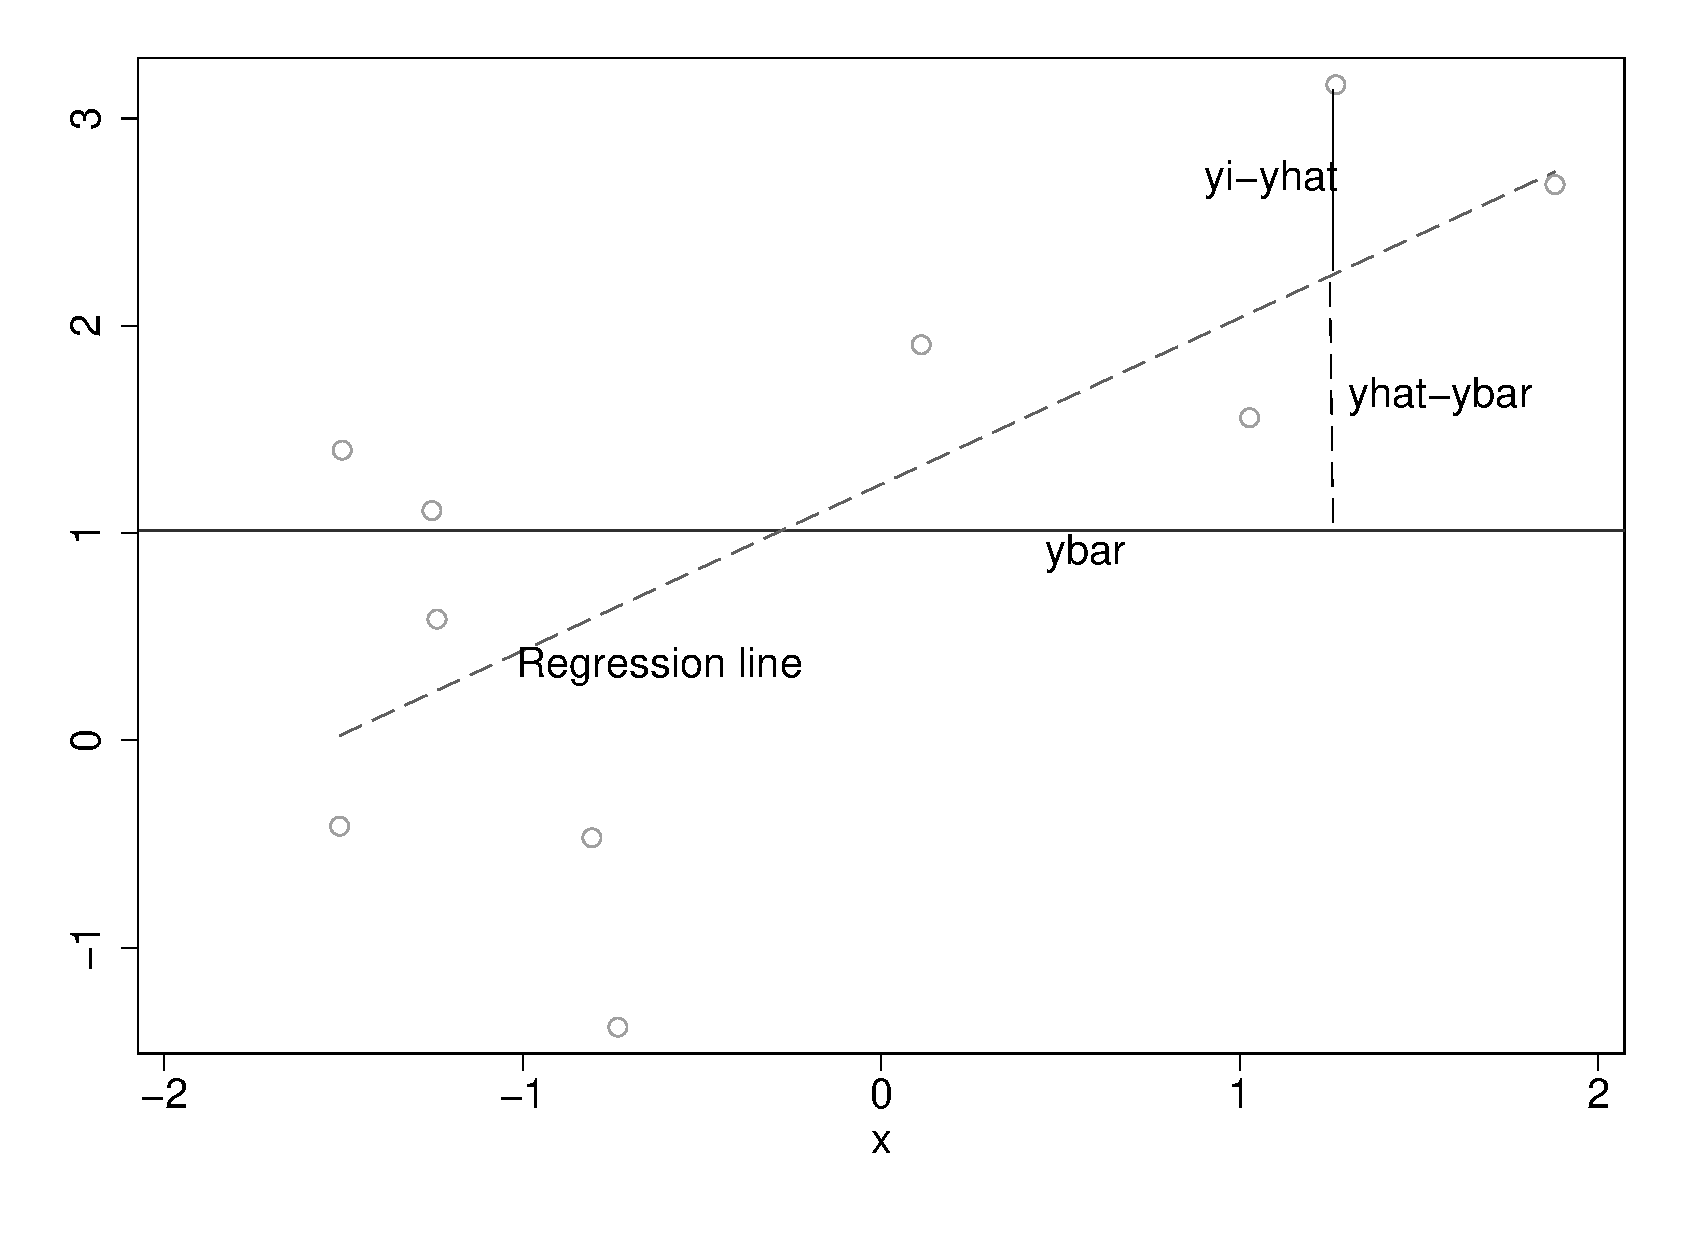
\includegraphics[angle=0,
           width=.75\textwidth]{anova.eps}
   \caption{The deviance of $y_i$ to $\hat{y}_i$ to $\bar{y}$}
  \label{fig:anova}
\end{figure}
This is visualized in Figure~\ref{fig:anova}, which is data from Table~\ref{tab:xy}. The solid line on the scatter plot is the overall mean of $y$, the dotted line with the slope is the regression fit line. We then take a single point and draw a solid vertical line from that point and the regression line. This represents $y_i-\hat{y}_i$. We then draw a dotted line from the predicted value of the regression line to the overall mean. This represents $\hat{y}_i-\bar{y}$ . The total difference between the observation and and the overall mean, $y_i-\bar{y}$, is the sum of these quantities.

With these quantities we can do an F-test to test whether the sum of squares residual is less than the sum of squares total
\begin{equation}
F=\frac{MSR}{MSE}
\end{equation}
where
\begin{equation}
MSR = \frac{SSR}{p}
\end{equation}
and
\begin{equation}
MSE = \frac{SSE}{N-p-1}
\end{equation}
This test is then evaluated against the F distribution with ($p, N-p-1$) degrees of freedom. The degrees of freedom for the sum of squares error is $N-p-1$, just like the $t$-test, and the degrees of freedom for the sum of squares regression is $p$, again where $p$ is the number of predictors excluding the intercept.

Examining the fit statistics from our wage and education example, Model 1 in Table~\ref{tab:wagereg_all}, the sum of squares from the model is 1,172.179 and the sum of squares error is 12,606.570. We then see the degrees of freedom ($df$) for each quantity. We can test the fit of the model with the $F$-test,
\[
F=\frac{\left(\frac{1172.179}{1}\right)}{\left(\frac{12606.570}{198}\right)}=18.410
\]
which is associated with a probability ($p$-value) of 0.00003. This should be familiar, that's because the unrounded $t$-test was 4.29, the square of which is 18.410. This means that our model contributes something to explaining the variation in wages.
\section{Model fit by way of $R^2$}
Another statistic reported in our regression output is $R^2$. Substantively, this is a measure of how much variation is "explained" in the data. The calculation for $R^2$ is simply the ratio of the sum of square regression to the sum of squares total ($SST = SSR + SSE$)
\begin{equation}
R^2 = \frac{SSR}{SSR+SSE}
\end{equation}

Since it is a ratio and $SSR$ is always smaller than $SST$, it ranges from 0 to 1, with better model fit as we approach 1. In the first model in Table~\ref{tab:wagereg_all}, education explains about 8.5 percent of the variation in wages. What is also interesting is that in bivariate regression $R^2$ is literally the square of the correlation coefficient. This means that education and wages have a correlation of $\sqrt{0.085} = 0.292$. In multiple regression, the meaning is a little bit vague, but can be thought of as the square of the correlation of all predictors and the outcome.

The adjusted R-square is a somewhat different formula that includes a penalty for adding several variables that are not correlated with the outcome. This is sometimes useful since R-squares will always increase with new variables and so we can fool ourselves with large R-squares by putting a lot of junk in the model. The formula is
\begin{equation}
R_{adjusted}^2=1-\left(\left(1-R^2\right)\frac{N-1}{N-p-1}\right)
\end{equation}
where $p$ is the number of predictors.
\section{Testing blocks of coefficients}
The $t$-tests of coefficients test each coefficient individually. This test is a test of whether that parameter is equal to 0. Another way to think of it is that it is a test of whether that variable adds to the explanatory power of the model compared to a model without that variable. This test compares the sum of squares error in the full model (or {\it unrestricted}) to the sum of squares error in the {\it restricted} model. For a single variable, this ratio is an F-test with ($1,N-p_U-1$) degrees of freedom, for more than 1 variable, the degrees of freedom are ($J_R,N-p_U-1$), where $J_R$ is the number of variables being tested and $p_U$ is the number of predictors (including the intercept) in the full model. The test is
\begin{equation}
F=\frac{\left(\frac{SSE_R-SSE_U}{J_R}\right)}{\left(\frac{SSE_U}{N-p_U-1}\right)}
\end{equation}
For example, Model 2 in Table~\ref{tab:wagereg_all} adds age as a predictor. The $t$-test indicates it is a significant predictor according to the three stars ($***$), but we can also find out with an $F$ test. Looking at the model statistics, we can call Model 1 the restricted model, so $SSE_R$ is 12606.570, and Model 2 the unrestricted model, so $SSR_U$ is 11175.277. Since the model adds a single variable, $J_R = 1$, and $N-3-1 = 200-2-1 = 196$. Thus, our test is
\[
F=\frac{\left(\frac{12606.570-11175.277}{1}\right)}{\left(\frac{11175.277}{196}\right)}
\]
\[
F=\frac{1431.293}{57.017}
\]
\[
F=25.103
\]
With ($1,196$) degrees of freedom, the probability of observing this test is 0.00001, which is very significant. We can check our work by estimating the $t$-test on the age effect:
\[
t=\frac{0.218}{0.043}
\]
\[
t=5.070
\]
the square of which is almost the same number as the $F$ test (differences due to rounding).

Model 3 in Table~\ref{tab:wagereg_all} adds the effect of gender. However, this effect is not significant.

Looks like gender ($female$) isn't significant, but does it add to the explanatory power of the model?

\section{Model Likelihood}
\label{sec:lrtest}

Since the least squares estimator is the same as the maximum likelihood estimator for normally distributed outcomes, OLS models have log-likelihood functions that get maximized, see section~\ref{sec:regml}.
Computers generally store the model likelihood along with other model statistics. With these we can perform likelihood ratio tests that compare different models on the same data. The ratio-test is
\begin{equation}\label{eq:lrtest}
\chi^2=2\left(\mbox{ln}\left(L\left(\theta_a\right)\right)-\mbox{ln}\left(L\left(\theta_{null}\right)\right)\right)
\end{equation}
when comparing the results of two likelihood functions (the value is evaluated on the $\chi^2$ distribution of a single degree of freedom). There is an example of this test in \ref{sec:likelihoodtest}.

\section{Important assumptions of OLS regression}
The formulas discussed in the previous sections make several assumptions. You'll find that a lot of statistical theory starts with "assume..." then "we can think of this relationship as..." Assumptions form the basis of any statistical analysis. Often, the new methods that come out are a result of data breaking some assumption so a new method needs to be created. In fact, most of these notes are about what to do when you break these assumptions. Thus, it is important to understand these assumptions.
\subsection{$y$ is a linear function of the predictors}
The first assumption is important for interpretation. We assume that $y$ is a linear function function of the predictors. When this is true, graphs tend to look like Figure~\ref{fig:linearok}.
\begin{figure}
   \centering
   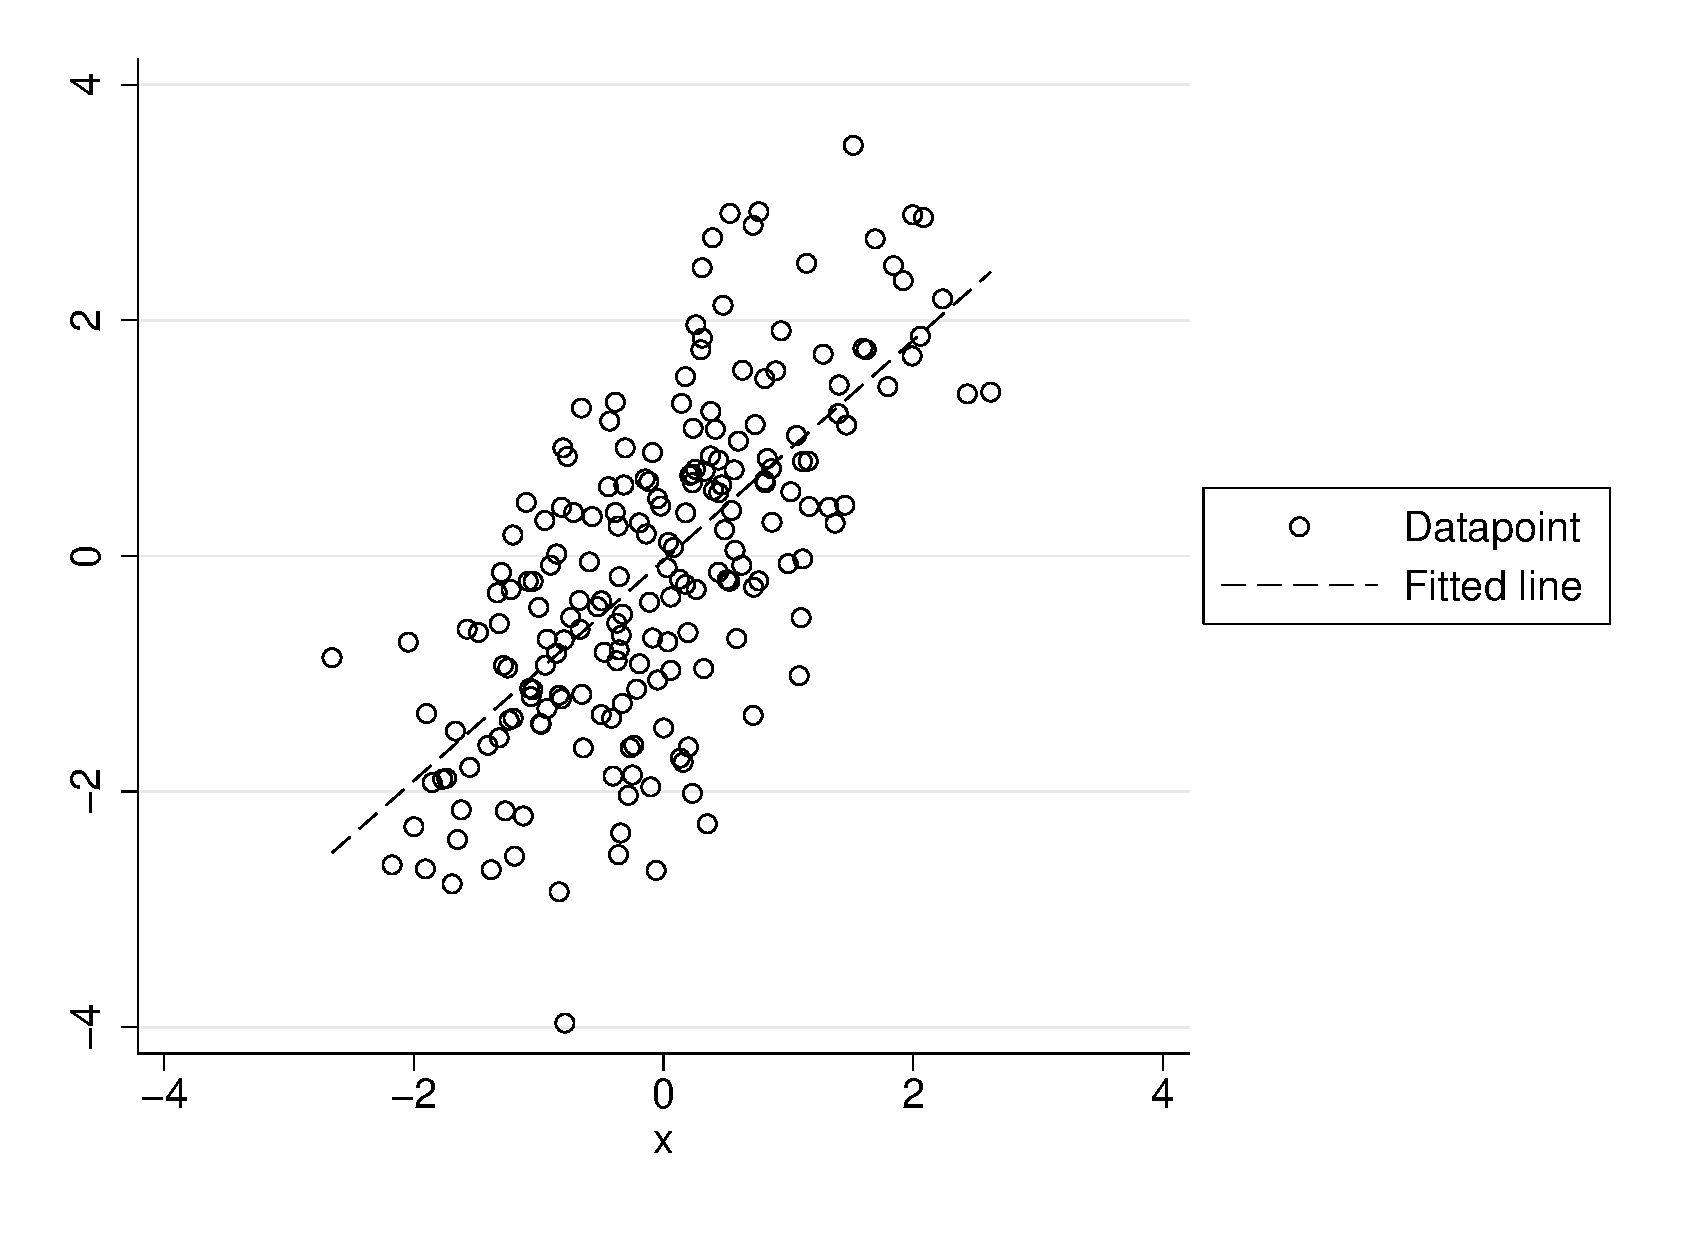
\includegraphics[angle=0,
           width=.75\textwidth]{linearok.eps}
   \caption{Data where $y$ is a linear function of $x$}
  \label{fig:linearok}
\end{figure}
In many cases relationships are not linear and if you do not transform the data the estimated relationships are not valid. A classic violation of this is a quadratic relationship.
\begin{figure}
   \centering
   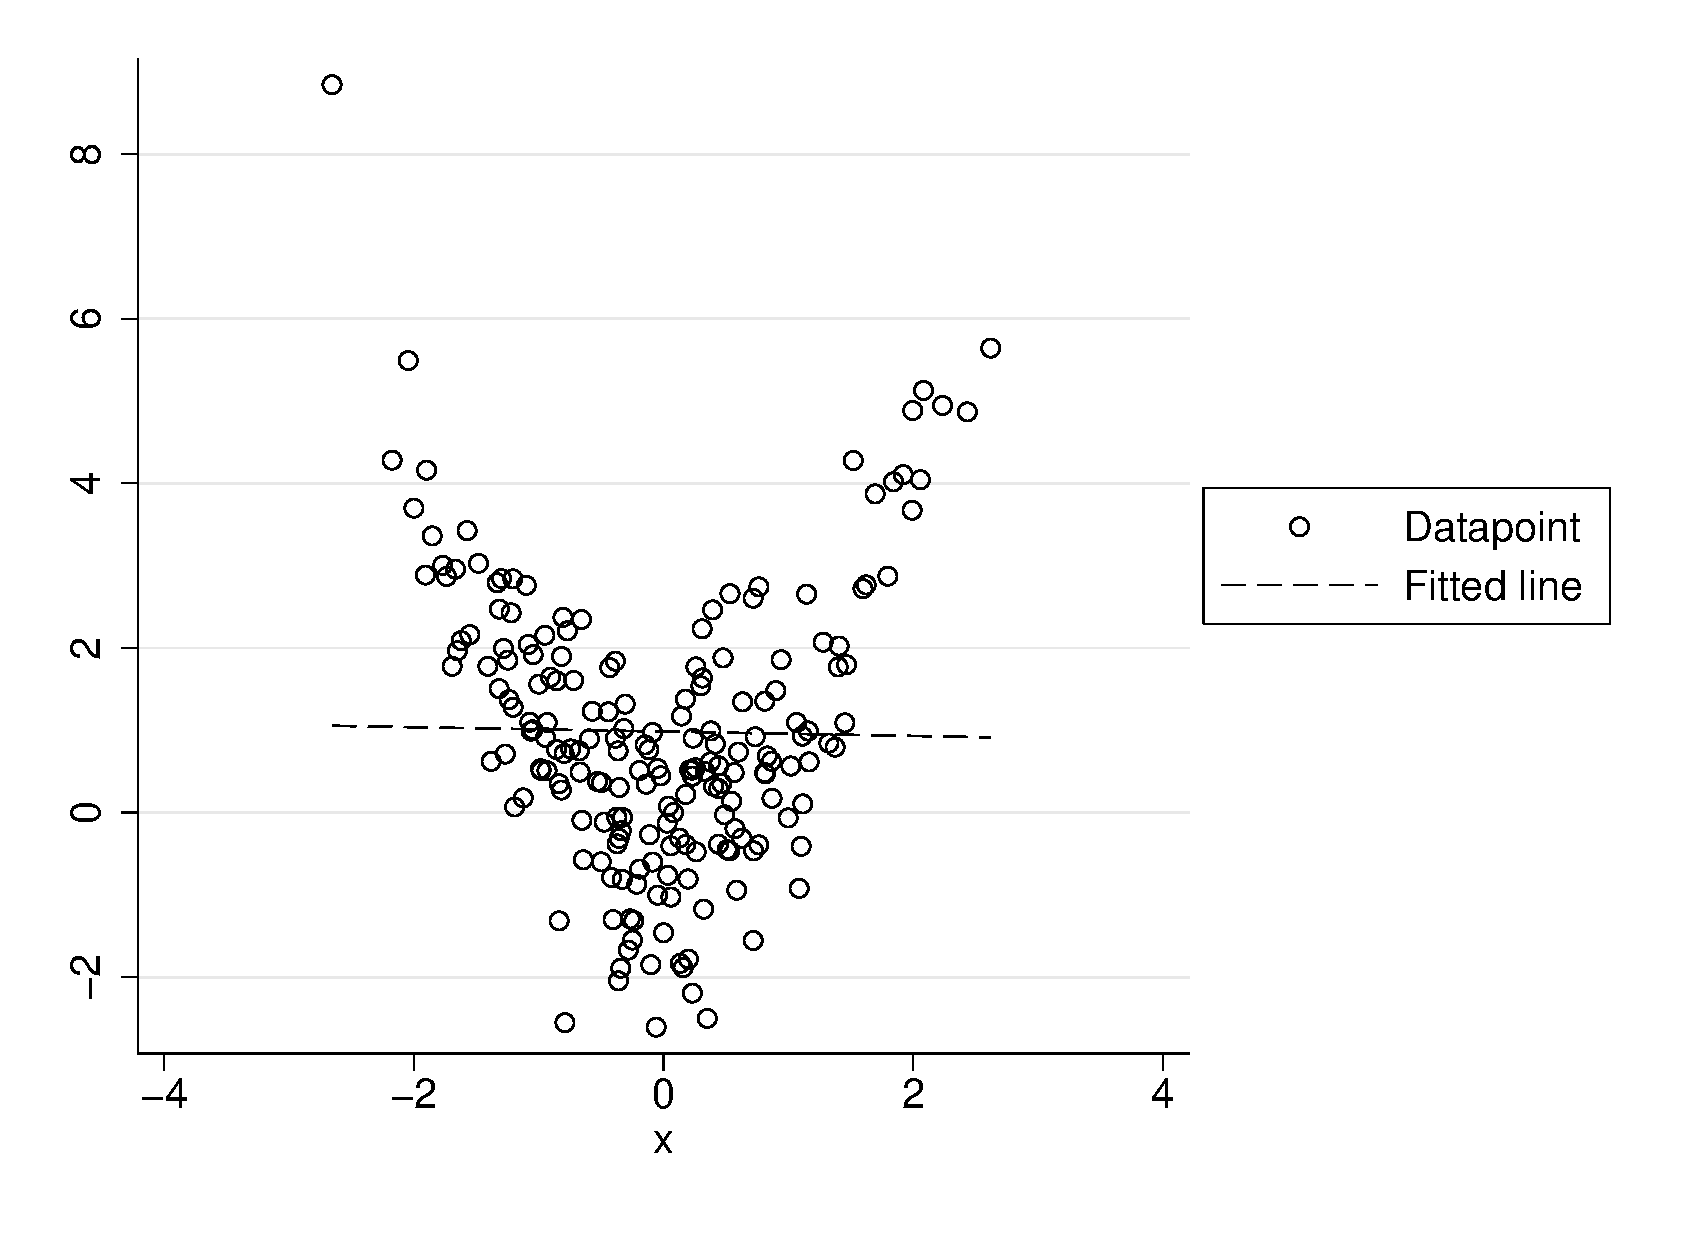
\includegraphics[angle=0,
           width=.75\textwidth]{linearnotok.eps}
   \caption{Data where $y$ is not a linear function of $x$}
  \label{fig:linearnotok}
\end{figure}
Figure~\ref{fig:linearnotok} displays this situation. When the relationship is quadratic and you fit a linear model without transformations, the slope may not reflect the data. In this case, the fitted slope is close to 0 even though it is obvious there is a relationship in the data.
Unfortunately, there is no easy way to check this assumption outside of a examining the data. This is why we have theory. The best regression diagnostic is theory. Your model should be governed by theory. Trust your theory.
\subsection{The expected value of any residual is zero}
Related to the previous assumption is that we assume that the expected value of a residual is 0. "Expected" is fancy statistics language for "average." Thus, we expect that the residuals to be 0, on average, for any level of predictor. The math forces this to be true overall. However, I find more nuanced way of thinking of this assumption is to assume that for every value of x, the expected value of the residuals is 0. If we have a multivariate model, then instead of x we can use the fitted value of y.
\begin{figure}
   \centering
   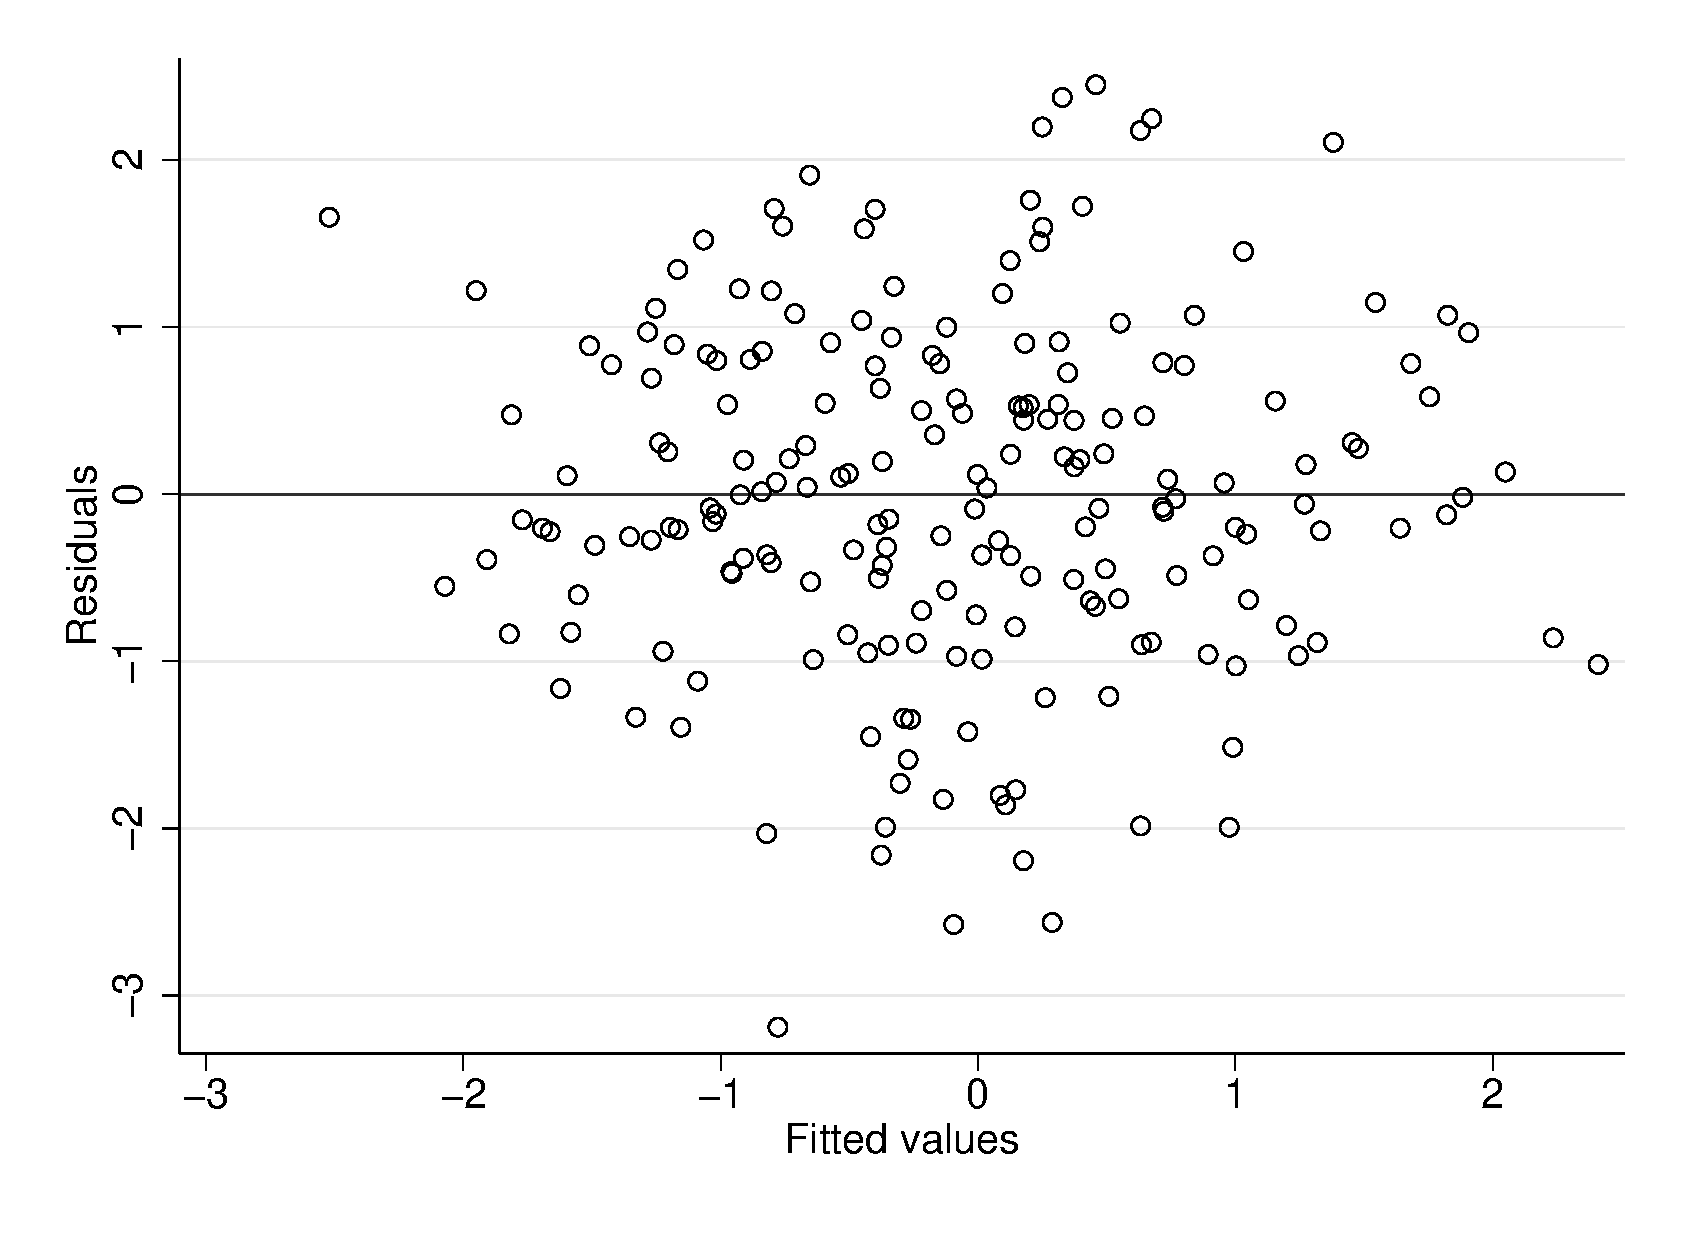
\includegraphics[angle=0,
           width=.75\textwidth]{mean0ok.eps}
   \caption{Data where $e$ is zero on average}
  \label{fig:mean0ok}
\end{figure}
The reason we can use a fitted value of y is that the fitted value of y is just a linear combination of all the predictors. We can inspect this visually by making a scatterplot of the residuals by the fitted values, see Figure~\ref{fig:mean0ok} where we meet the assumption that residuals average to 0. If, on the other hand, there is some pattern to the residuals, like in a un-modeled quadratic relationship, the plot may look like Figure~\ref{fig:mean0notok}.
\begin{figure}
   \centering
   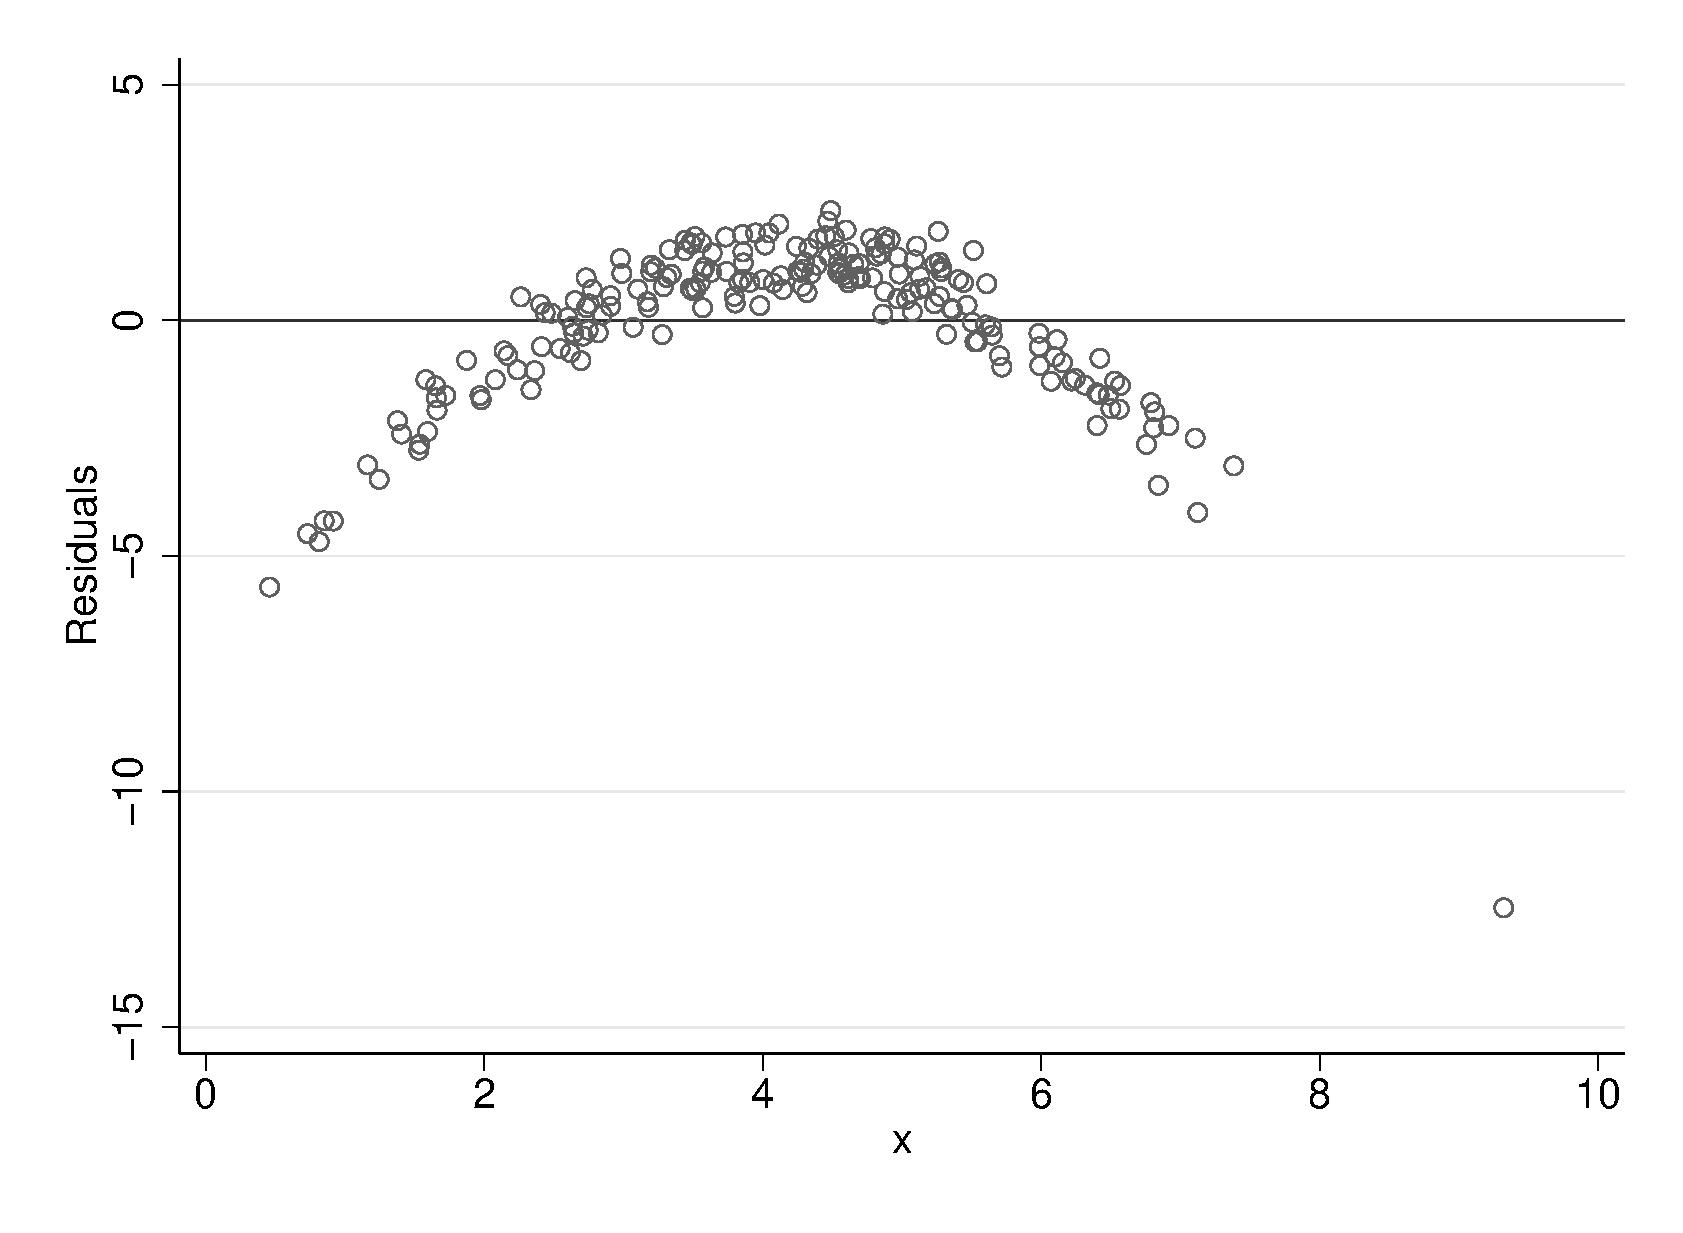
\includegraphics[angle=0,
           width=.75\textwidth]{mean0notok.eps}
   \caption{Data where $e$ is not zero on average}
  \label{fig:mean0notok}
\end{figure}
\subsection{The variance of the residuals is constant}
As we will see throughout the book, many of the formulas for standard errors and other measures make the assumption that there is a single variance for all the residuals, $\sigma^2$.

However, in many situations this is not the case. When this assumption is violated, standard error become biased, making hypothesis tests difficult. Often this happens for practical reasons. For example, we will look at an example where charitable giving is a function of income. When income is low, there is little variance in giving because those who do not have a lot of money cannot give anything. At the other end, there is quite a bit of variance: you have people like Bill Gates who give a lot, and people like Steve Jobs who did not give much (at least publicly). When this is violated, you may see a "fan" pattern in your residuals like in Figure~\ref{fig:hetero}
\begin{figure}
   \centering
   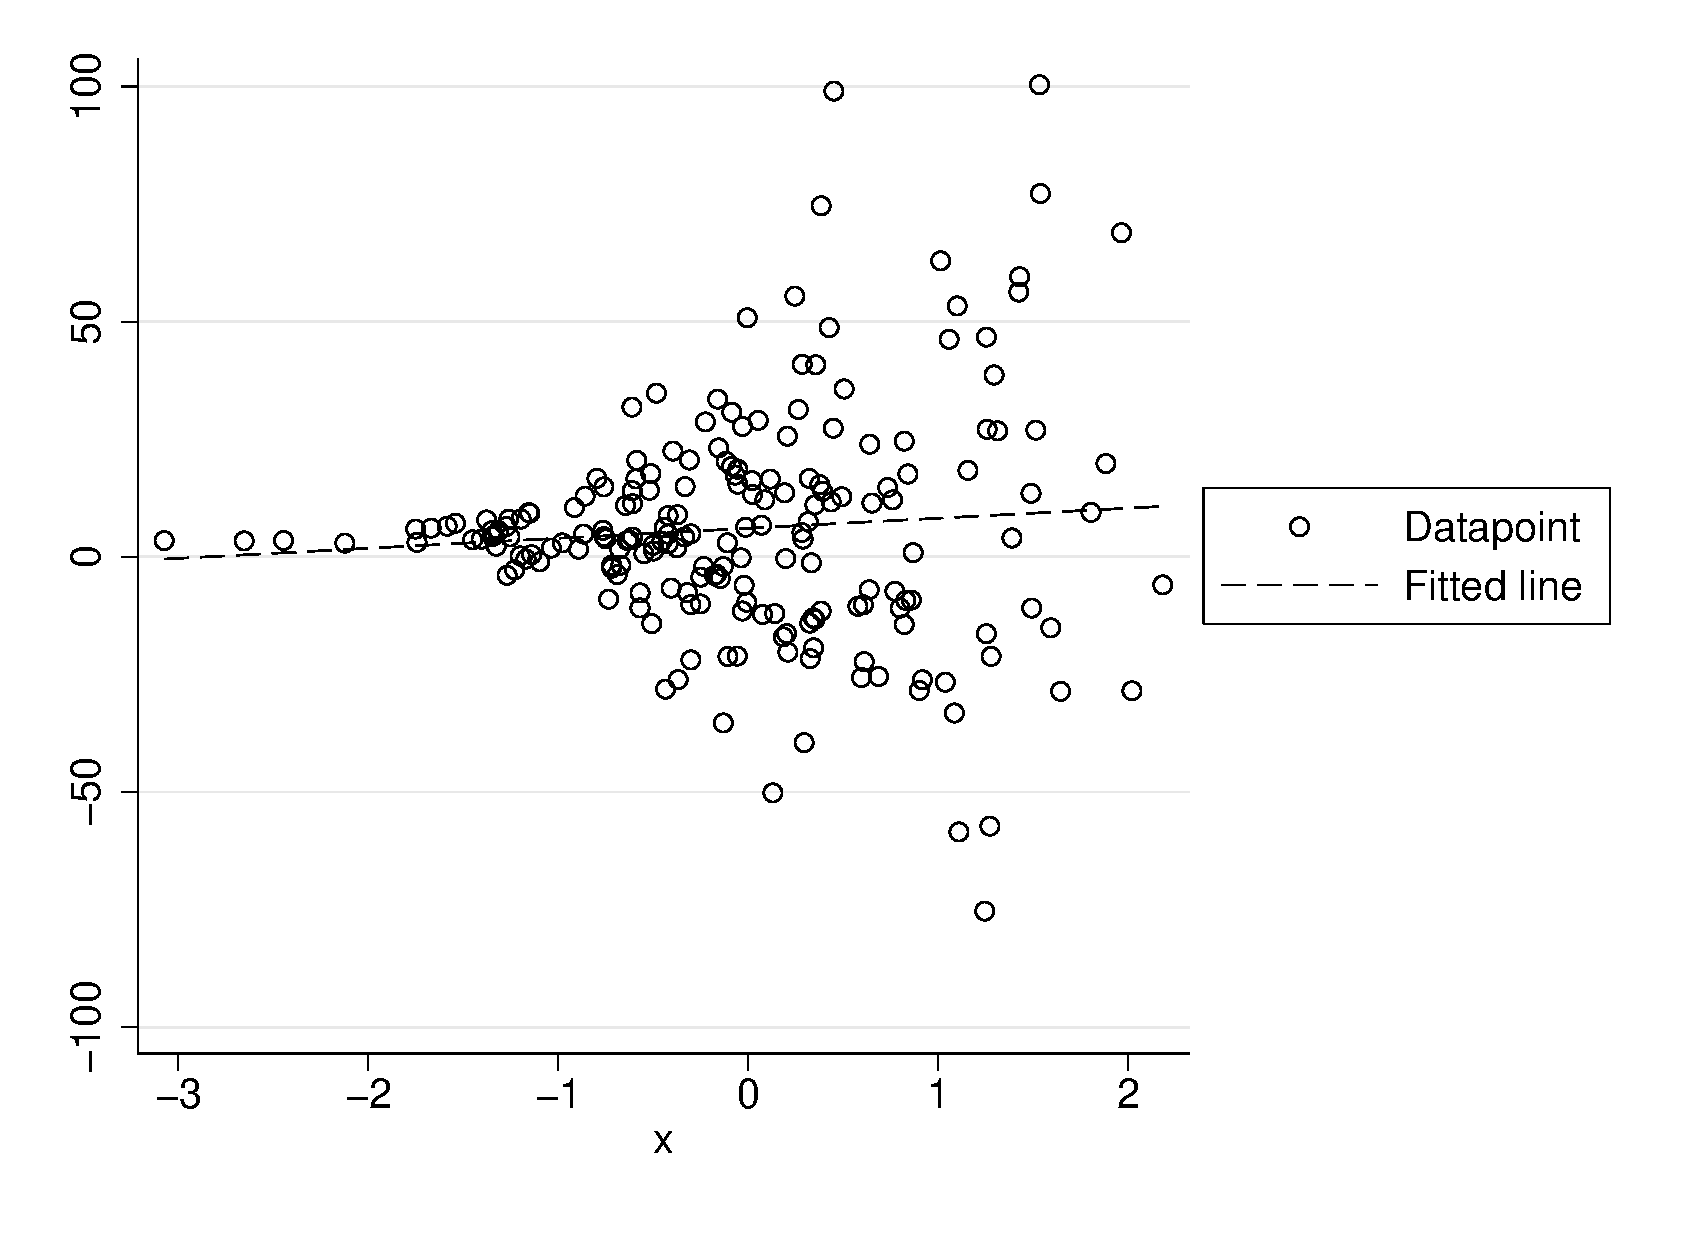
\includegraphics[angle=0,
           width=.75\textwidth]{hetero.eps}
   \caption{Data where $e$ does not have constant variance}
  \label{fig:hetero}
\end{figure}
\subsection{The covariance of all residuals is zero}
One of the most commonly violated assumptions is that all the residuals are independent. We can express this as
\begin{equation}
\mbox{cov}\left(e_i,e_j\right)=0
\end{equation}
There are several ways in which observations of y can be correlated:
\begin{enumerate}
 \item Observations are adjacent to each other across time
 \item Observations are members of common geographical regions
 \item Observations are members of other common meaningful clusters
 \item Any combination of the above, and more
\end{enumerate}
This is an old problem in social science and survey research. There are many solutions to this issue and we cover many of them in these notes.
\subsection{The values of the predictors are not random}
In normal regression we assume that the predictors, especially the intercept, are not random variables.  When we cluster sample, that is sample groups then units within those groups, the intercept can be argued to be a random variable and thus violating this assumption.  Another example is time within units.  Many of the multilevel models are designed to compensate for this issue.
\subsection{The values of the predictors are not exact linear combinations of each other}
This assumption is pretty easy to confirm. If it is violated, and one variable is exactly correlated with another, it is impossible in invert . Many software packages with automatically remove offending variables from models.
\subsection{The errors are distributed normally}
Many students misunderstand this assumption to mean that the outcome needs to be distributed normally. This is not the case. The residuals, the outcome net of the model, must be normally distributed.
For example, consider a model a continuous predictor $x$ and another dichotomous predictor $z$. A histogram of the data appears in Figure~\ref{fig:dummyhist} and you can see the bi-modal distribution. We see in Figure~\ref{fig:dummyhist_r} that net of the model the errors are almost normally distributed. We need to make this assumption to prove that the least squares estimator is the maximum likelihood estimator.
\begin{figure}
   \centering
   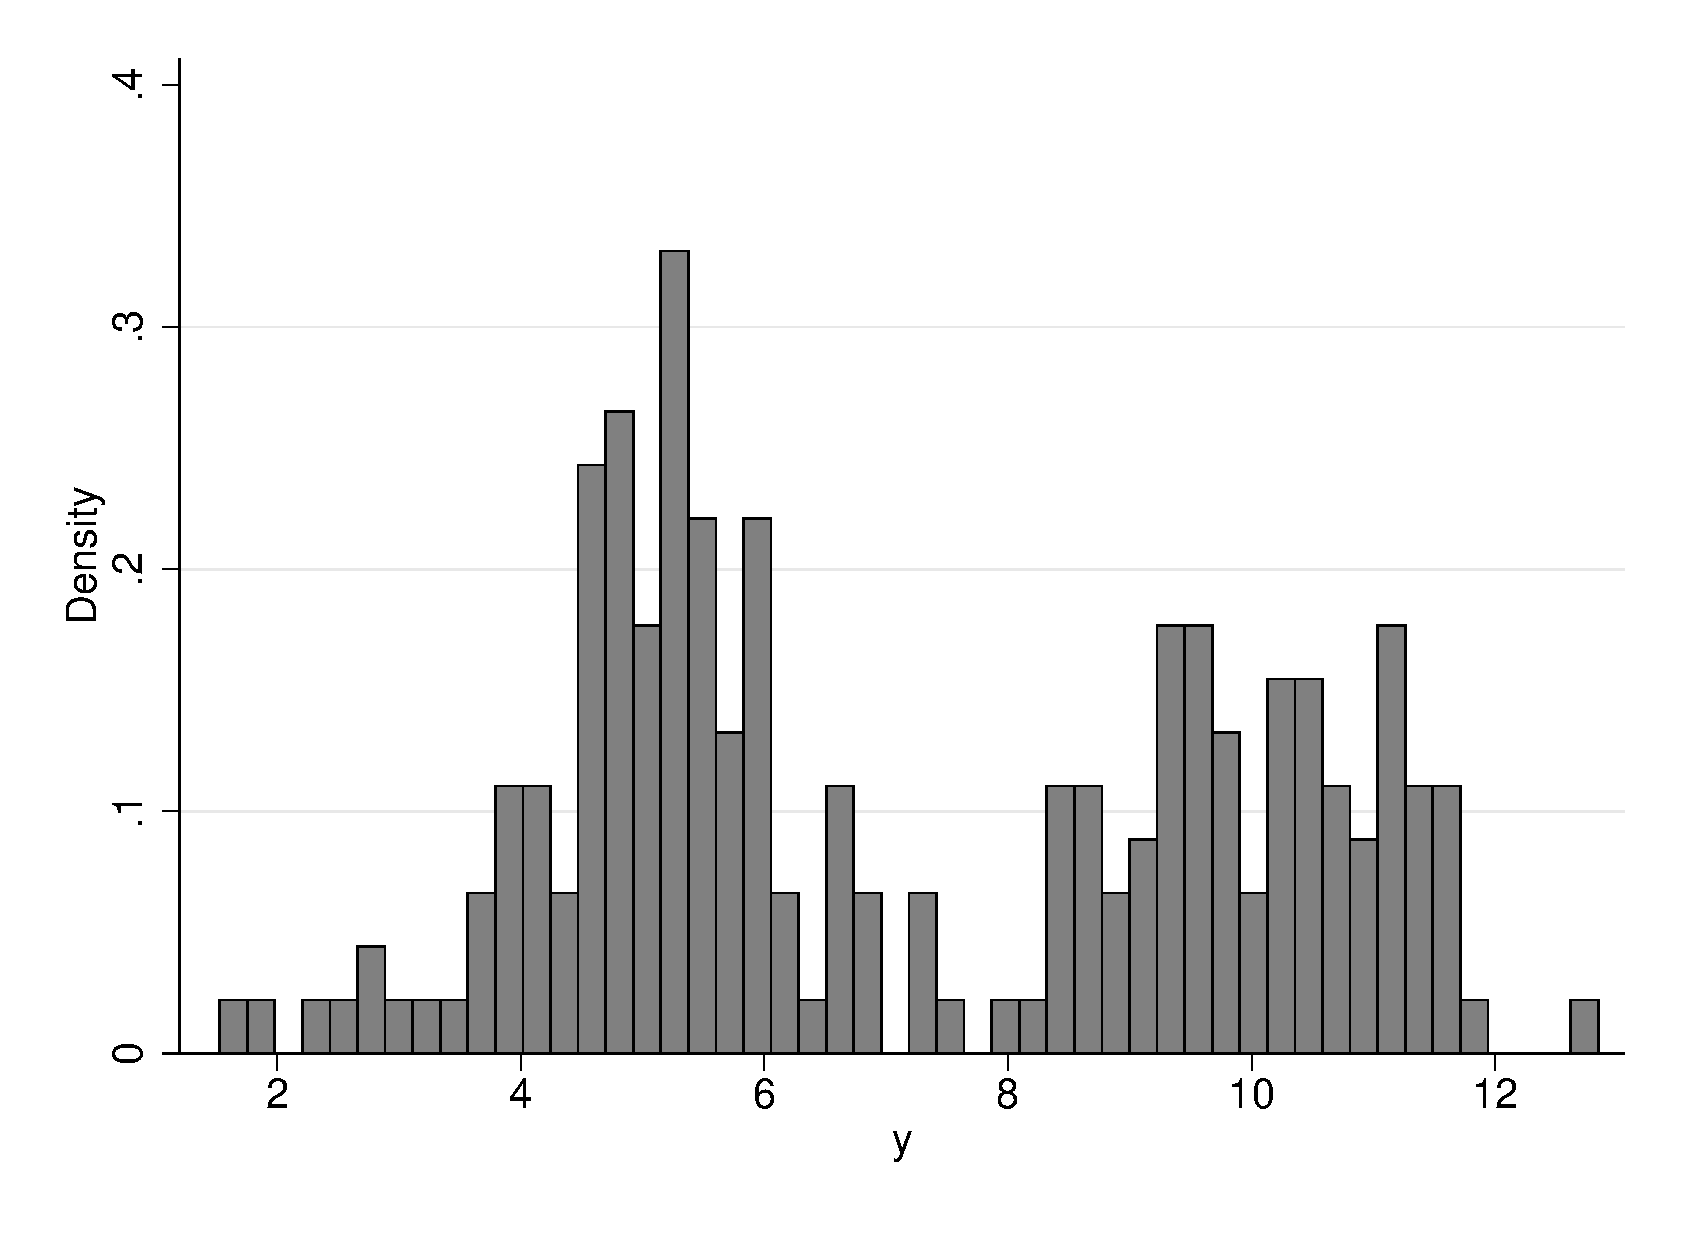
\includegraphics[angle=0,
           width=.75\textwidth]{dummyhist.eps}
   \caption{Data $y$ as a function of a dummy variable}
  \label{fig:dummyhist}
\end{figure}
\begin{figure}
   \centering
   \includegraphics[angle=0,
           width=.75\textwidth]{dummyhist_r.eps}
   \caption{Residuals of a model for $y$ that included a dummy variable}
  \label{fig:dummyhist_r}
\end{figure}

However, sometimes there is no way to achieve normal errors. Situations in which the outcome is dichotomous or a count variable with a large proportion of zeros will never produce normally distributed outcomes. In those situations we need to use generalized linear models (GLMs).

\section*{For more information}
For OLS regression inference and diagnostics, see \citep{fox}. For model evaluation and diagnostics, consult \citep{hill}. Power analysis for regression is covered in \citep{cohen1988statistical} and \citep{maxwell2008sample}.



\chapter{Colinearity}\citep{fox}

Colinearity among predictors is an interesting problem in regression. From one point of view, it is a scourge that reduces the precision of estimates and can make our coefficients unstable. From another point of view, it is the reason we perform multiple regression in the first place. The following offers an explicit example of the problem. Note, however, the actual issue is often less obvious.

I will first describe how it creates problem for precision, as it is an interesting discussion. From there, there really is not much to write about, since most "solutions" are pretty cheap and don't work that well.

\section{Perfect colinearity}

If two predictors in the model are perfectly correlated, they must be measuring the exact same thing. Therefore, it does not make sense to put the same information into the model twice. Don't worry about inadvertently making this mistake, as the {\bf X'X} matrix will not be able to be inverted in this case and your software will produce an error.

\section{Non-perfect colinearity}

This leaves us with the more plausible issue. In any case, two variable in your model are likely to be correlated {\it at least a little bit}. This follows simple logic that if $x$ and $z$ are correlated with $y$, then there must be at least some relationship between $x$ and $z$, even if it is just a little bit.

Again, there is nothing wrong with this, since this is why we want to perform multiple regression in the first place. However, there are limits to how much correlation we can have among our predictors.

\subsection{The variance inflation factor}

Recall from section~\ref{sec:matrixv} that in the bivariate case the variance of the regression coefficient is equation~\eqref{eq:olsb1var}
\[
\mbox{var}\left(\beta_1\right)=\frac{\sigma^2}{\sum_{i=1}^N\left(x_i-\bar{x}\right)^2}
\]
this can be extended to the multiple regression case for slope $j$ of predictor $j$ by adding the variance inflation factor (VIF), $\frac{1}{1-R^2_j}$, to the formula
\begin{equation}\label{eq:olsb1varwvif}
\mbox{var}\left(\beta_j\right)=\frac{1}{1-R^2_j}\frac{\sigma^2}{\left(N-1\right)s^2_j}
\end{equation}
The VIF is literally what it sounds like, its the extent to which (or factor of) the variance of a predictor is increased, given the multiple correlation between it and the other predictors.

Here, $R^2_j$ is the key ingredient. $R^2_j$ is like any other $R^2$ statistic, except here it is how much of predictor $j$ is explained by the {\it other predictors}. The larger $R^2_j$, the larger the variance (and standard error) of $\beta_j$.\footnote{Note, also that since $s^2$ is the variance, we can return to the sum of squares my multiplying the variance by $N-1$.}


\begin{figure}
   \centering
   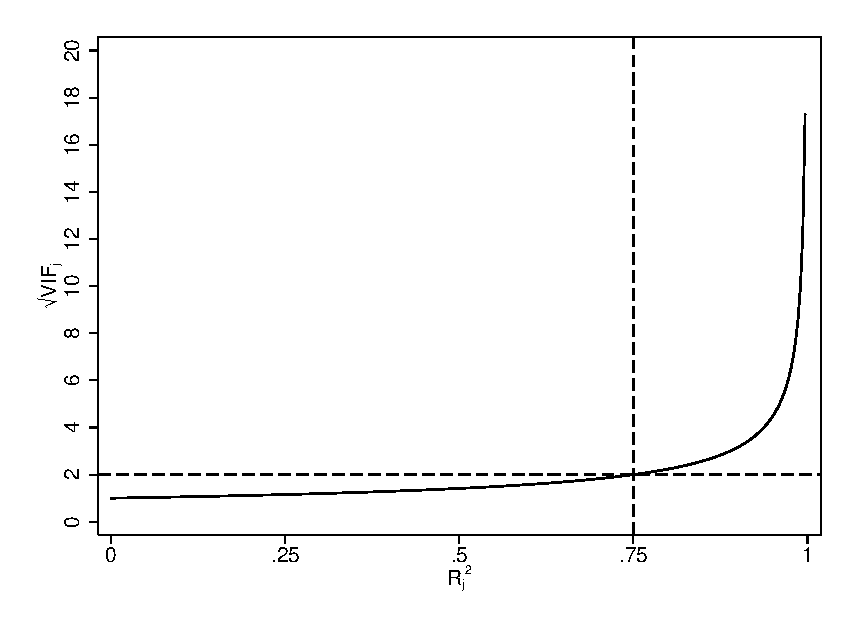
\includegraphics[angle=0,
           width=1\textwidth]{vif.eps}
   \caption{Relationship between the variance inflation factor and $R^2_j$}
  \label{fig:vif}
\end{figure}

But how much is too much correlation among the predictors? Consider Figure~\ref{fig:vif}, where we plot the square root of the VIF against the value of $R^2_j$. Note that the standard error doubles when $R^2_j$ is 0.75. That is, our standard errors only double when three fourths of the variation in one variable is explained by the other predictors. After that, things get worse pretty fast.

\subsection{Example with city data}

The example that follows is pretty silly, but it highlights the issues that you can encounter with high levels of multicolinearity. Suppose the data in Table~\ref{tab:rentdata}, at the end of this chapter. It's census data from the 1980s and includes the average rent, average family income, median household income, and percent of the population with a college degree for various rural places.

Table~\ref{tab:rentcorr} provides the correlations and Figure~\ref{fig:rentmatrix} is a scatter plot matrix of these variables. As you can see, and expectedly, mean family income and median household income are highly correlated.

\begin{table}[htbp]\centering
 \caption{Correlations of variables in Table~\ref{tab:rentdata}
\label{tab:rentcorr}}
\begin{tabular}{lcccc}
\hline
& Mean & Mean family & Median & Percent \\
& rent & income & household & with BA \\
& & & income & \\
\hline
Mean rent & 1.00 \\
Mean family income & 0.63 & 1.00 \\
Median household income & 0.66 & 0.96 & 1.00 \\
Percent with BA & 0.58 & 0.81 & 0.72 & 1.00 \\
\hline
\end{tabular}
\end{table}

An analysis of these data has a simple hypothesis, that higher the family income, holding education constant, the higher rent should be. Now, examine model 1 in Table~\ref{tab:rentmodel}, mean family income has a negative (and significant) slope. This is the other thing that can happen with highly correlated predictors, the sign can flip.

This isn't to say that the model is {\it wrong}, but we have to take it literally: holding the median constant, if the mean increases (i.e. the data become more skewed), rent decreases.

This, however, is not a useful analysis. The better option is to select either the mean family income or the median household income as we do in Models 2 and 3.

The discussion of VIFs can inform the difference in the significance of the effect of education between Model 2 and 3. Notice how, in Table~\ref{tab:rentcorr} that the percent with a college degree is more correlated with mean family income. That correlation is 0.8132, which translates into a VIF of
\[
VIF = \frac{1}{1-R^2_j} = \frac{1}{1-0.8132^2}=2.95
\]
making the effect of education not significant.

However, the correlation with the median income is lower, 0.7238, with a VIF of only 2.10, and the effect of education is now significant.
\[
VIF = \frac{1}{1-R^2_j} = \frac{1}{1-0.7238^2}=2.10
\]

\begin{figure}
   \centering
   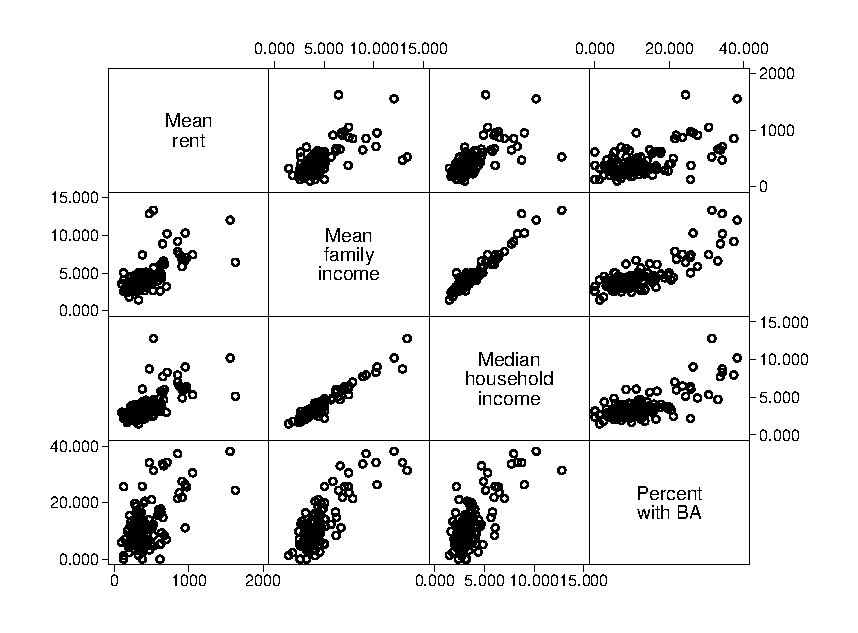
\includegraphics[angle=0,
           width=1\textwidth]{rent_corr.eps}
   \caption{Scatter matrix of variables in Table~\ref{tab:rentdata}}
  \label{fig:rentmatrix}
\end{figure}

\begin{table}[htbp]\centering
 \caption{Models predicting mean rent in census places Table~\ref{tab:rentdata}
\label{tab:rentmodel}}
\begin{tabular}{lccc}
\hline
Variable      &    Model 1 & Model 2 & Model 3 \\
\hline
Mean family income  &   -79.636* &   56.360***&        \\
      &  (38.517)  &  (14.952)  &        \\
Median household income  &   140.822***&        &   69.508***\\
      &  (37.090)  &        &  (13.827)  \\
Percent with BA  &   0.111** &    0.060  &    0.064* \\
      &   (0.037)  &   (0.036)  &   (0.029)  \\
Intercept  &   133.748** &   106.433* &   96.588* \\
      &  (43.034)  &  (44.795)  &  (39.645)  \\
\hline
\multicolumn{4}{l}{Model Statistics} \\
\hline
N      &   120.000  &   120.000  &   120.000  \\
F      &   34.683  &   40.206  &   48.528  \\
$R^2$    &    0.473  &    0.407  &    0.453  \\
$df$ Regression     &    3.000  &    2.000  &    2.000  \\
Sum of Squares Regression     & 3548574.288  & 3056921.326  & 3402777.993  \\
$df$ Error     &   116.000  &   117.000  &   117.000  \\
Sum of Squares Error     & 3956217.179  & 4447870.140  & 4102013.473  \\
\hline
\multicolumn{4}{l}{Variance Inflation Factors} \\
\hline
Mean Income & 21.81 & 2.95 & \\
Median Income & 15.55 & & 2.10 \\
Percent with BA & 3.40 & 2.95 & 2.10 \\
\hline
\multicolumn{4}{l}{$SE$s in parentheses, $*p<0.05,**p<0.01,***p<0.001$} \\
\hline
\end{tabular}
\end{table}

\subsection{What to do?}
There are essentially two things you can do to solve colinearity:
\begin{itemize}
\item{drop variables}
\item{combine variables}
\end{itemize}

\subsubsection{Drop variables}
This is essentially what we did in Models 2 and 3 in Table~\ref{tab:rentmodel}. Since we can make the argument that both income variables are essentially measuring the same thing, we just pick one and be done with it.

\subsubsection{Combine variables}
The other option is to use factor analysis (which is beyond the scope of these notes for now) to create a common factor score that combines the information from the predictors which are highly correlated.

\section*{For more information}
For treatment of multicollinearity in regression, see \citep{fox} and \citep{hill}. For comprehensive regression analysis, consult \citep{agresti} and \citep{cameron2005microeconometrics}.





\chapter{Outliers}

Data are not perfect. At times, we run into the problem of one case having more influence over the least squares line than other cases. In regression, we assume that each case exerts equal influence on the regression line. In some cases, a single extreme value of a predictor can change the entire regression line. For example, consider Figure~\ref{fig:xout}. The graph on the left is for well behaving data, and the graph on the right shows the effect of a single extreme $x$ variable. Things are not as bad if we have an extreme value on the outcome, however, as we see in Figure~\ref{fig:yout}.

\begin{figure}
   \centering
   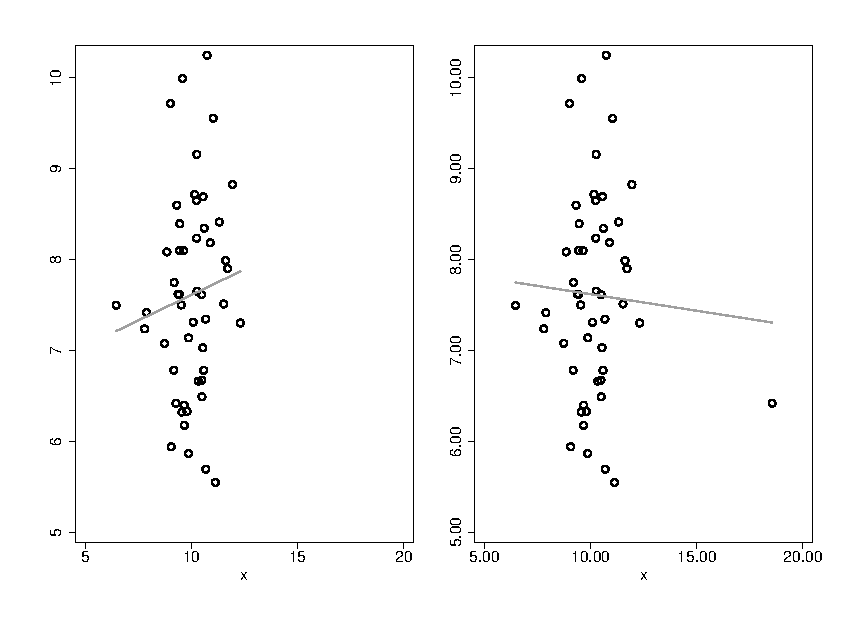
\includegraphics[angle=0,
           width=.75\textwidth]{xout.eps}
   \caption{Effect of extreme value of $x$}
  \label{fig:xout}
\end{figure}

\begin{figure}
   \centering
   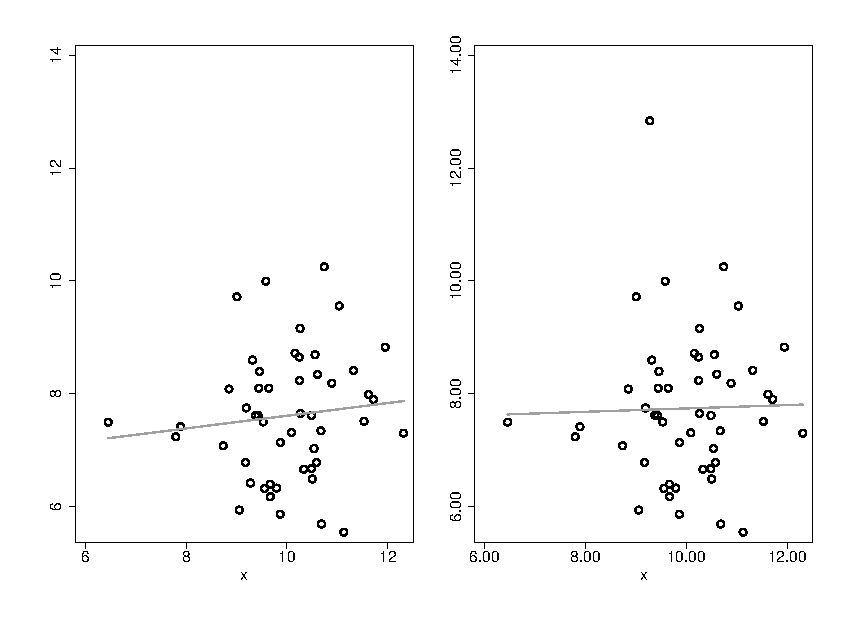
\includegraphics[angle=0,
           width=.75\textwidth]{yout.eps}
   \caption{Effect of extreme value of $y$}
  \label{fig:yout}
\end{figure}

Life isn’t so clear as these figures, however. How would be able to detect outlier variables when the number of cases are several hundred? Turns out there are a several different measures and tea-leaves to read. Let’s go over the favorites.

After you fit a model, there are about 6 big methods to detect outliers. These methods create a value for each case, and so these must be plotted for visual inspection. Generally by the case number, or "index."

As a reference, each measure plotted on normal data is displayed in Figure~\ref{fig:outnorm}.

\begin{figure}
   \centering
   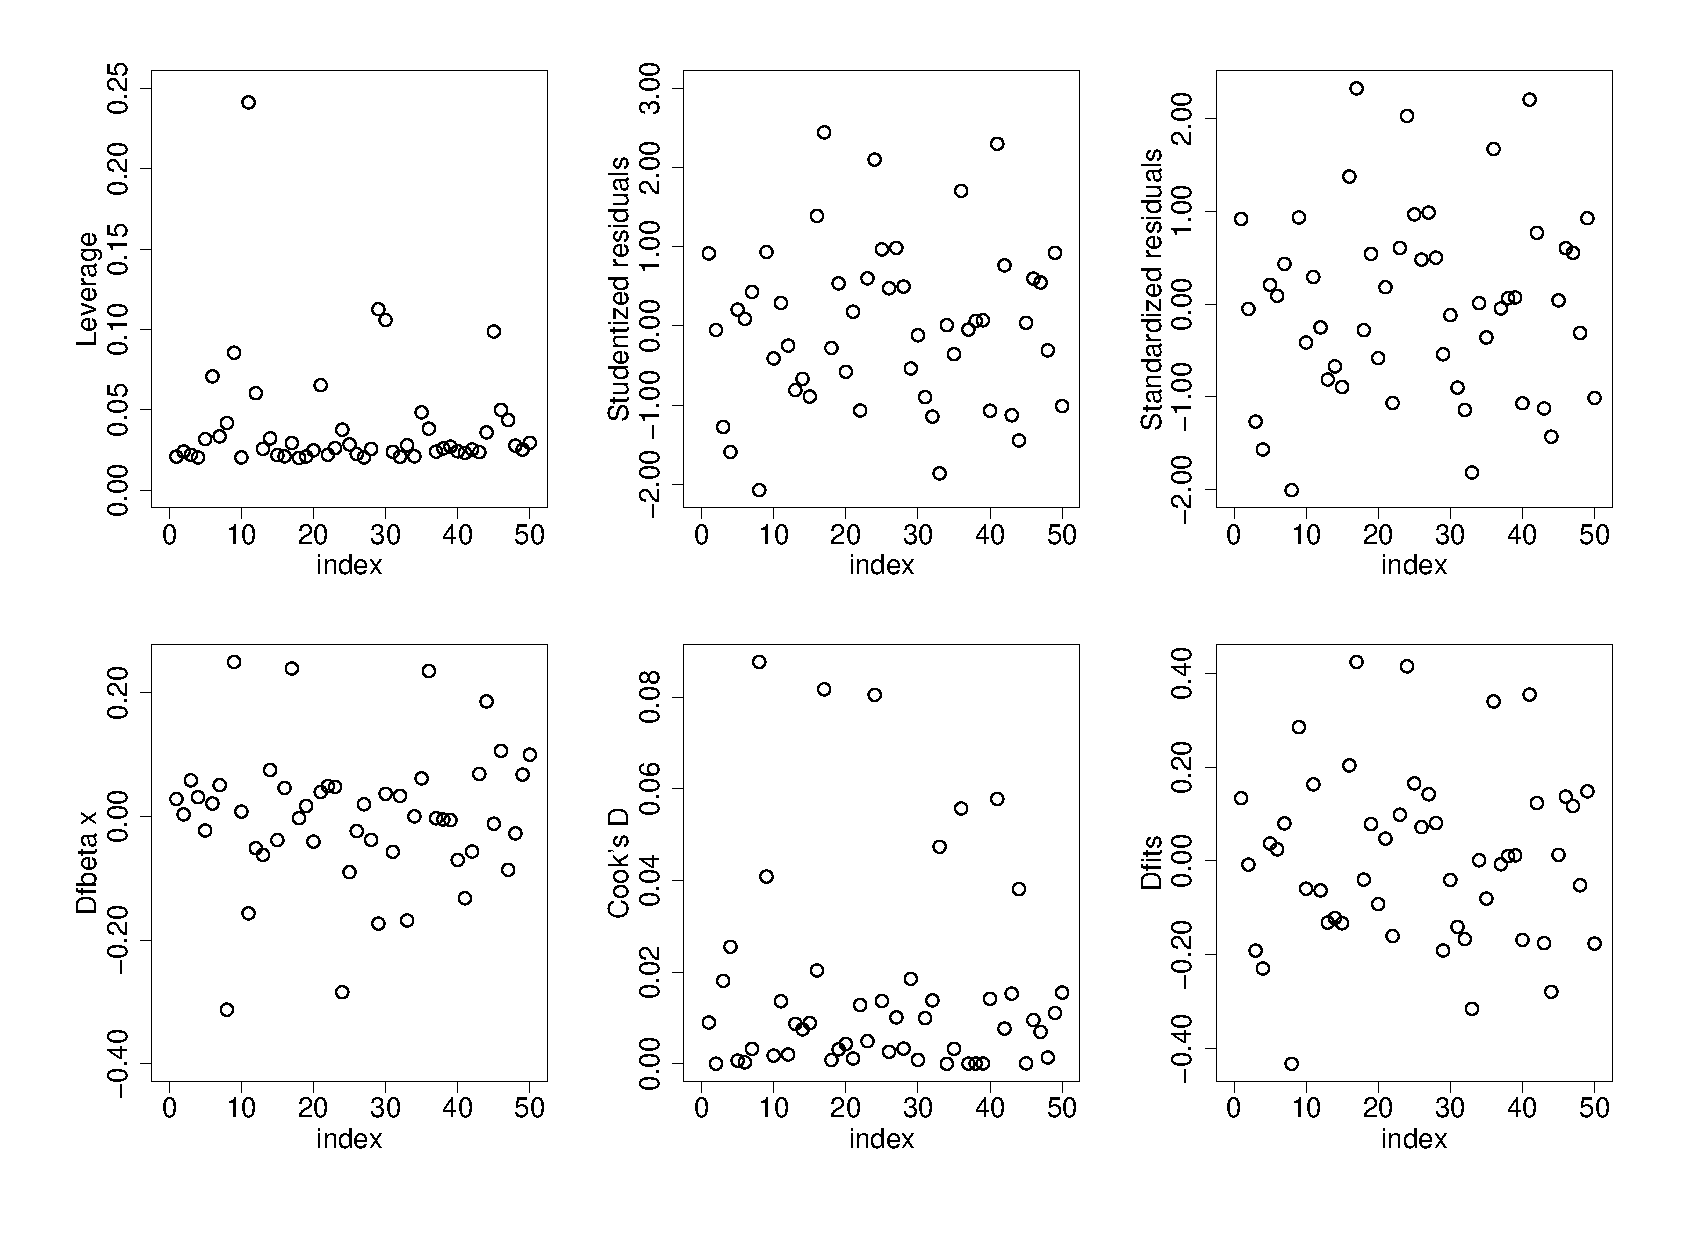
\includegraphics[angle=0,
           width=.75\textwidth]{normal_allmeasures_index.eps}
   \caption{Outlier values by case number of typical data in Table~\ref{tab:outdata}}
  \label{fig:outnorm}
\end{figure}

\section{Leverage}

If we examine the plots above, we can notice that outlier $x$ tend to drag the regression line around. This is called leverage. Leverage can be modeled by saying that each $j^{th}$ {\it fitted} value is a function of all the {\it observed} values of $y$,
\begin{equation}
\hat{y}_j=h_{1j}y_1+\ldots+h_{nj}y_n
\end{equation}
\begin{equation}
=\sum_{i=1}^N h_{ij}y_i
\end{equation}
In a simple bivariate regression, $h_j$ can be calculated with
\begin{equation}
h_j=\frac{1}{N}+\frac{\left(x_j-\bar{x}\right)^2}{\sum_{i=1}^N\left(x_i-\bar{x}\right)^2}
\end{equation}
For example, the calculations are shown in Table~\ref{tab:lever} for a small set of 5 cases.

\begin{table}[htbp]\centering
\caption{Example leverage calculations
\label{tab:lever}}
\begin{tabular}{lccc}
\hline
& $x$ & $\left(x-\bar{x}\right)^2$ & $h$ \\
\hline
&-0.960&0.006&0.201 \\
&-0.260&0.605&0.312 \\
&-3.020&3.928&0.930 \\
&-0.150&0.789&0.346 \\
&-0.800&0.057&0.211 \\
\hline
Sum & & 5.385 \\
Mean & -1.038 \\
\hline
\end{tabular}
\end{table}

If we examine the data in Table~\ref{tab:outdata} and plot the leverage values for the regression of $y$ on the $x$ column with the extreme case, you can see that case has a leverage value of 0.62 in Figure~ref{fig:xleverlab}.


\begin{figure}
   \centering
   \includegraphics[angle=0,
           width=.75\textwidth]{xout_hatvalues_label.eps}
   \caption{Scatter plot of data in Table~\ref{tab:outdata} ($y$ with extreme $x$) leverage values}
  \label{fig:xleverlab}
\end{figure}

However, a more useful method to detect which case(s) has (have) the extreme values is to plot the leverage value by case number, or {\it: index} as in Figure~\ref{fig:xlever}.

\begin{figure}
   \centering
   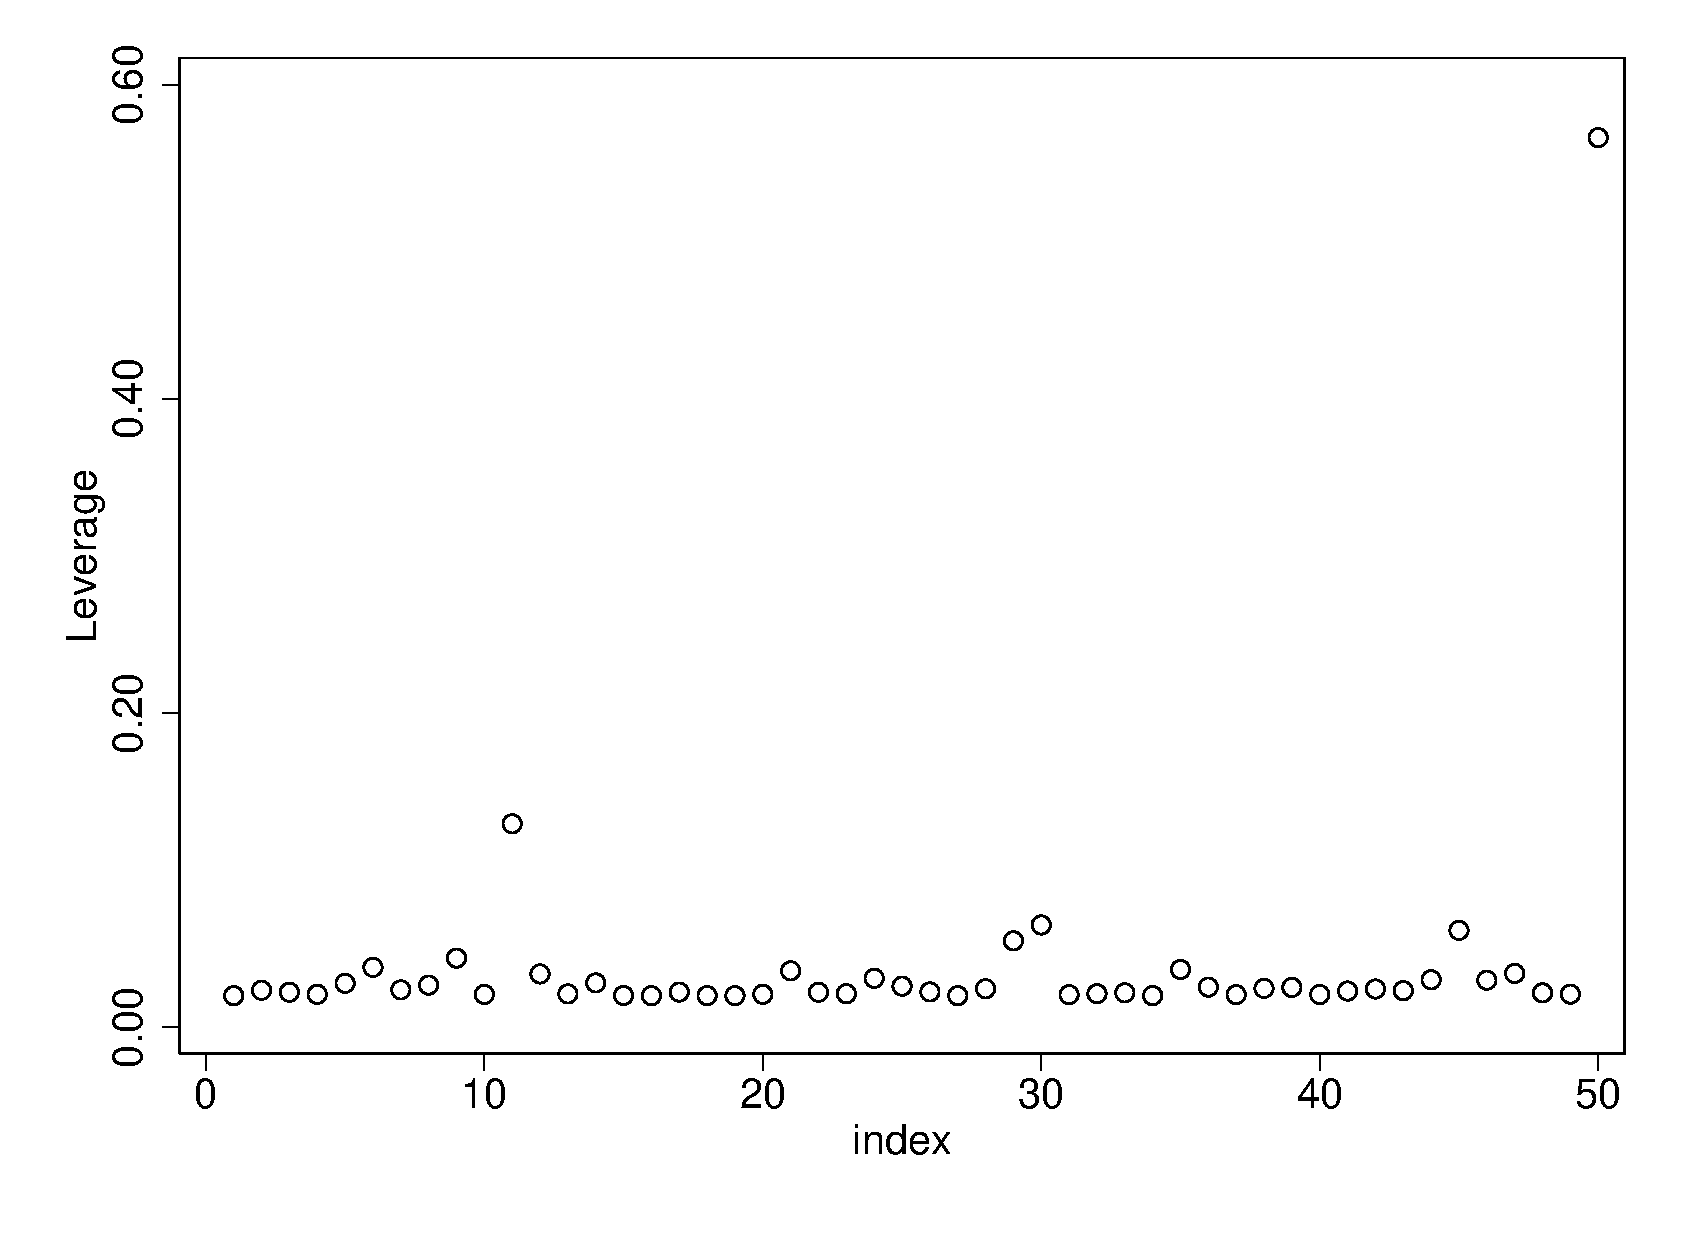
\includegraphics[angle=0,
           width=.75\textwidth]{xout_hatvalues_index.eps}
   \caption{Leverage values for extreme value of $x$ by case number of data in Table~\ref{tab:outdata}}
  \label{fig:xlever}
\end{figure}

As you can see in Figure~\ref{fig:ylever}, the leverage formulas have less utility in the cases of extreme $y$ values.

\begin{figure}
   \centering
   \includegraphics[angle=0,
           width=.75\textwidth]{yout_hatvalues_index.eps}
   \caption{Leverage values for extreme value of $y$ by case number of data in Table~\ref{tab:outdata}}
  \label{fig:ylever}
\end{figure}

\section{Standardized residuals}

Another plausible measure is the standardized residual from the model relative to the leverage, $h_i$

\begin{equation}
e^{\left(standardized\right)}_i=\frac{e_i}{s_e\sqrt{1-h_i}}
\end{equation}

where $s_e$ is the standard deviation of the residuals from the model. Figures with extraordinary values of $x$ and $y$ are displayed in Figures~\ref{fig:xstandard} and ~\ref{fig:ystandard}, respectively.

\begin{figure}
   \centering
   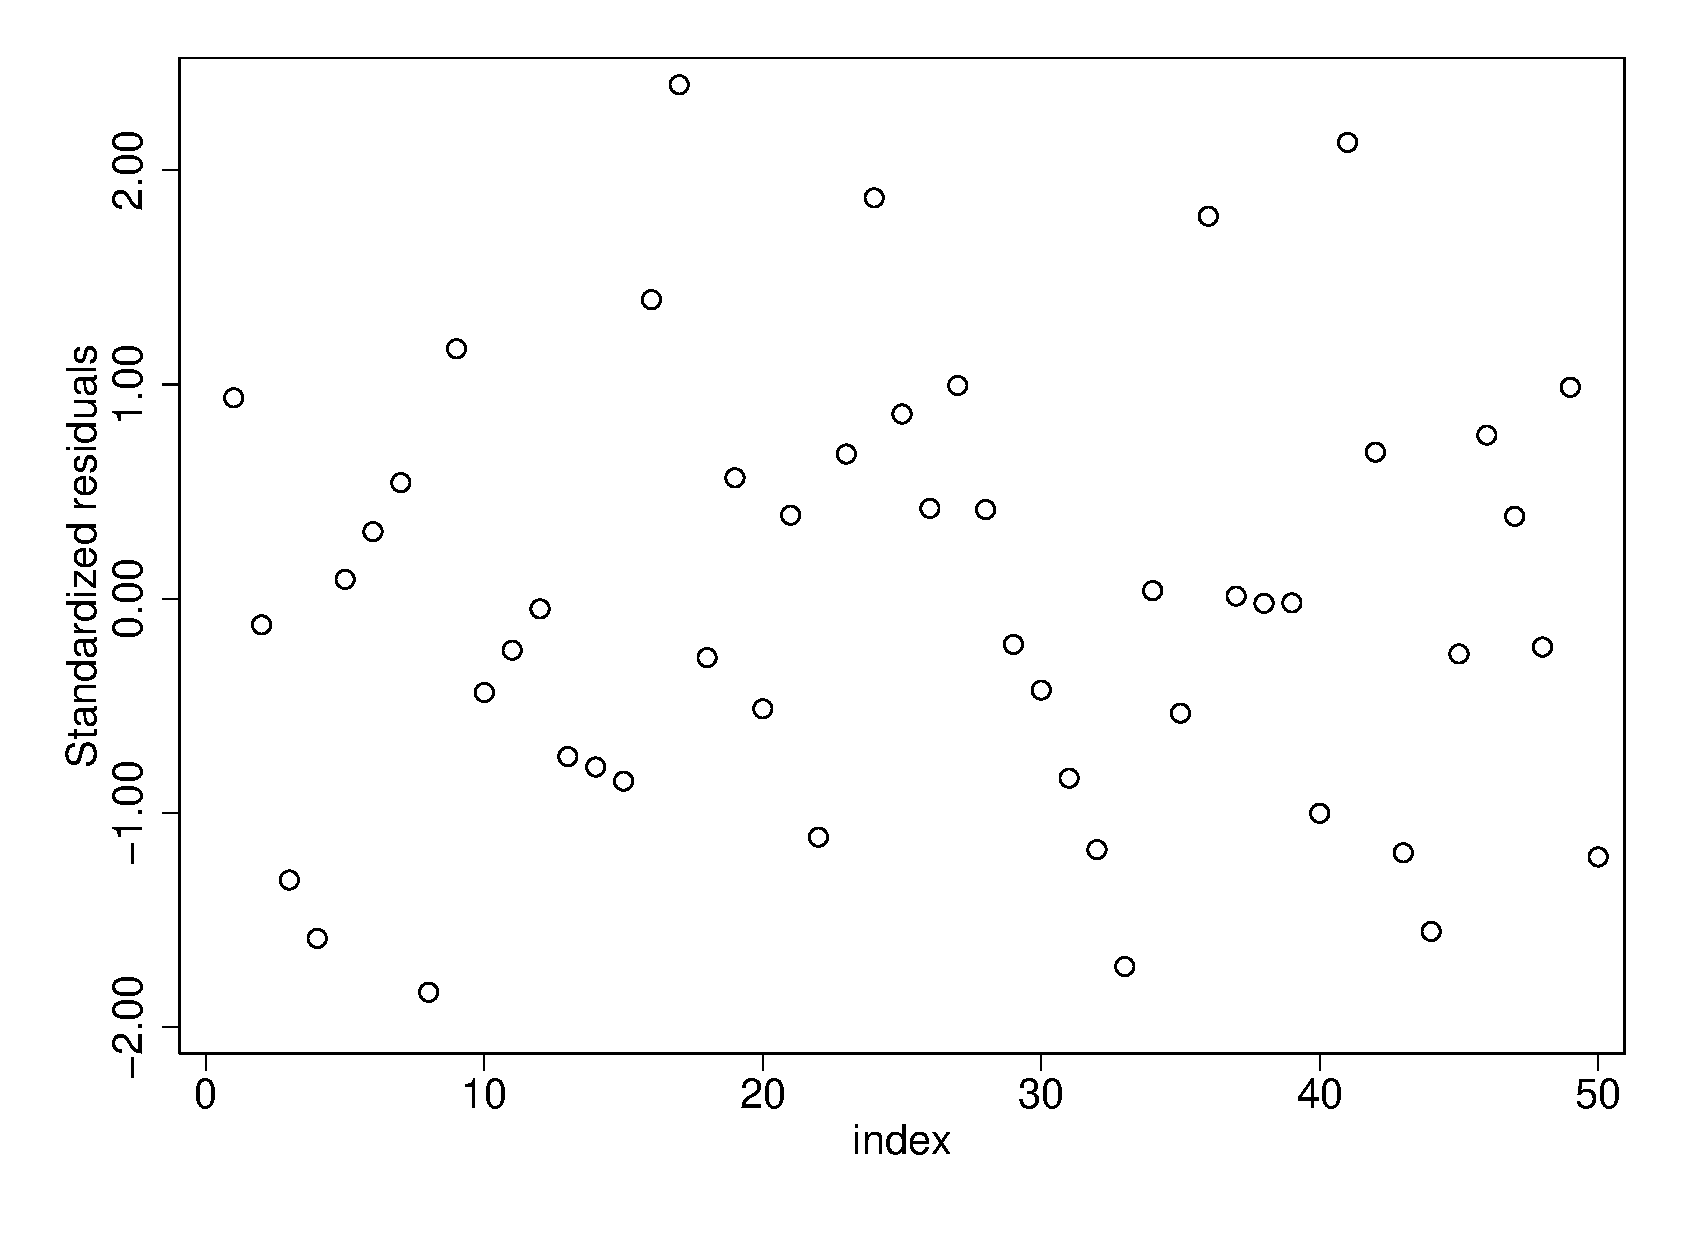
\includegraphics[angle=0,
           width=.75\textwidth]{xout_standard_index.eps}
   \caption{Standardized residual values for extreme value of $x$ by case number of data in Table~\ref{tab:outdata}}
  \label{fig:xstandard}
\end{figure}

\begin{figure}
   \centering
   \includegraphics[angle=0,
           width=.75\textwidth]{yout_standard_index.eps}
   \caption{Standardized residual values for extreme value of $y$ by case number of data in Table~\ref{tab:outdata}}
  \label{fig:ystandard}
\end{figure}

\section{Studentized residuals}

Another approach to residuals is to employ a standard deviation of the results from a model that excludes a particular case. Thus, for a given case $i$, this residual is
\begin{equation}
e^{\left(studentized\right)}_i=\frac{e_i}{s^{\left(-i\right)}_e\sqrt{1-h_i}}
\end{equation}
Figures with extraordinary values of $x$ and $y$ are displayed in Figures~\ref{fig:xstudent} and ~\ref{fig:ystudent}, respectively.
\begin{figure}
   \centering
   \includegraphics[angle=0,
           width=.75\textwidth]{xout_student_index.eps}
   \caption{Studentized residual values for extreme value of $x$ by case number of data in Table~\ref{tab:outdata}}
  \label{fig:xstudent}
\end{figure}

\begin{figure}
   \centering
   \includegraphics[angle=0,
           width=.75\textwidth]{yout_student_index.eps}
   \caption{Studentized residual values for extreme value of $y$ by case number of data in Table~\ref{tab:outdata}}
  \label{fig:ystudent}
\end{figure}


\section{DFBETA}

Yet another way to think about outliers is not how they influence the errors, but instead how they influence the regression slopes.
Thus, the DFBETA. This is the difference in a regression slope for predictor $p$ if a particular case $i$ was removed
\begin{equation}
D_{pi}=\beta_p - \beta_p^{-i}
\end{equation}

\begin{figure}
   \centering
   \includegraphics[angle=0,
           width=.75\textwidth]{xout_dfb_index.eps}
   \caption{Df-Beta values for extreme value of $x$ by case number of data in Table~\ref{tab:outdata}}
  \label{fig:xdfb}
\end{figure}

\begin{figure}
   \centering
   \includegraphics[angle=0,
           width=.75\textwidth]{yout_dfb_index.eps}
   \caption{Df-Beta values for extreme value of $y$ by case number of data in Table~\ref{tab:outdata}}
  \label{fig:ydfb}
\end{figure}

Figures with extraordinary values of $x$ and $y$ are displayed in Figures~\ref{fig:xdfb} and ~\ref{fig:ydfb}, respectively.

\section{Cook's distance}

The Cook's distance measure combines the leverage values with standardized residuals
\begin{equation}
D_i = \frac{e^{\left(standardized\right)}_i}{k+1}\times\frac{h_i}{1-h_i}
\end{equation}


\begin{figure}
   \centering
   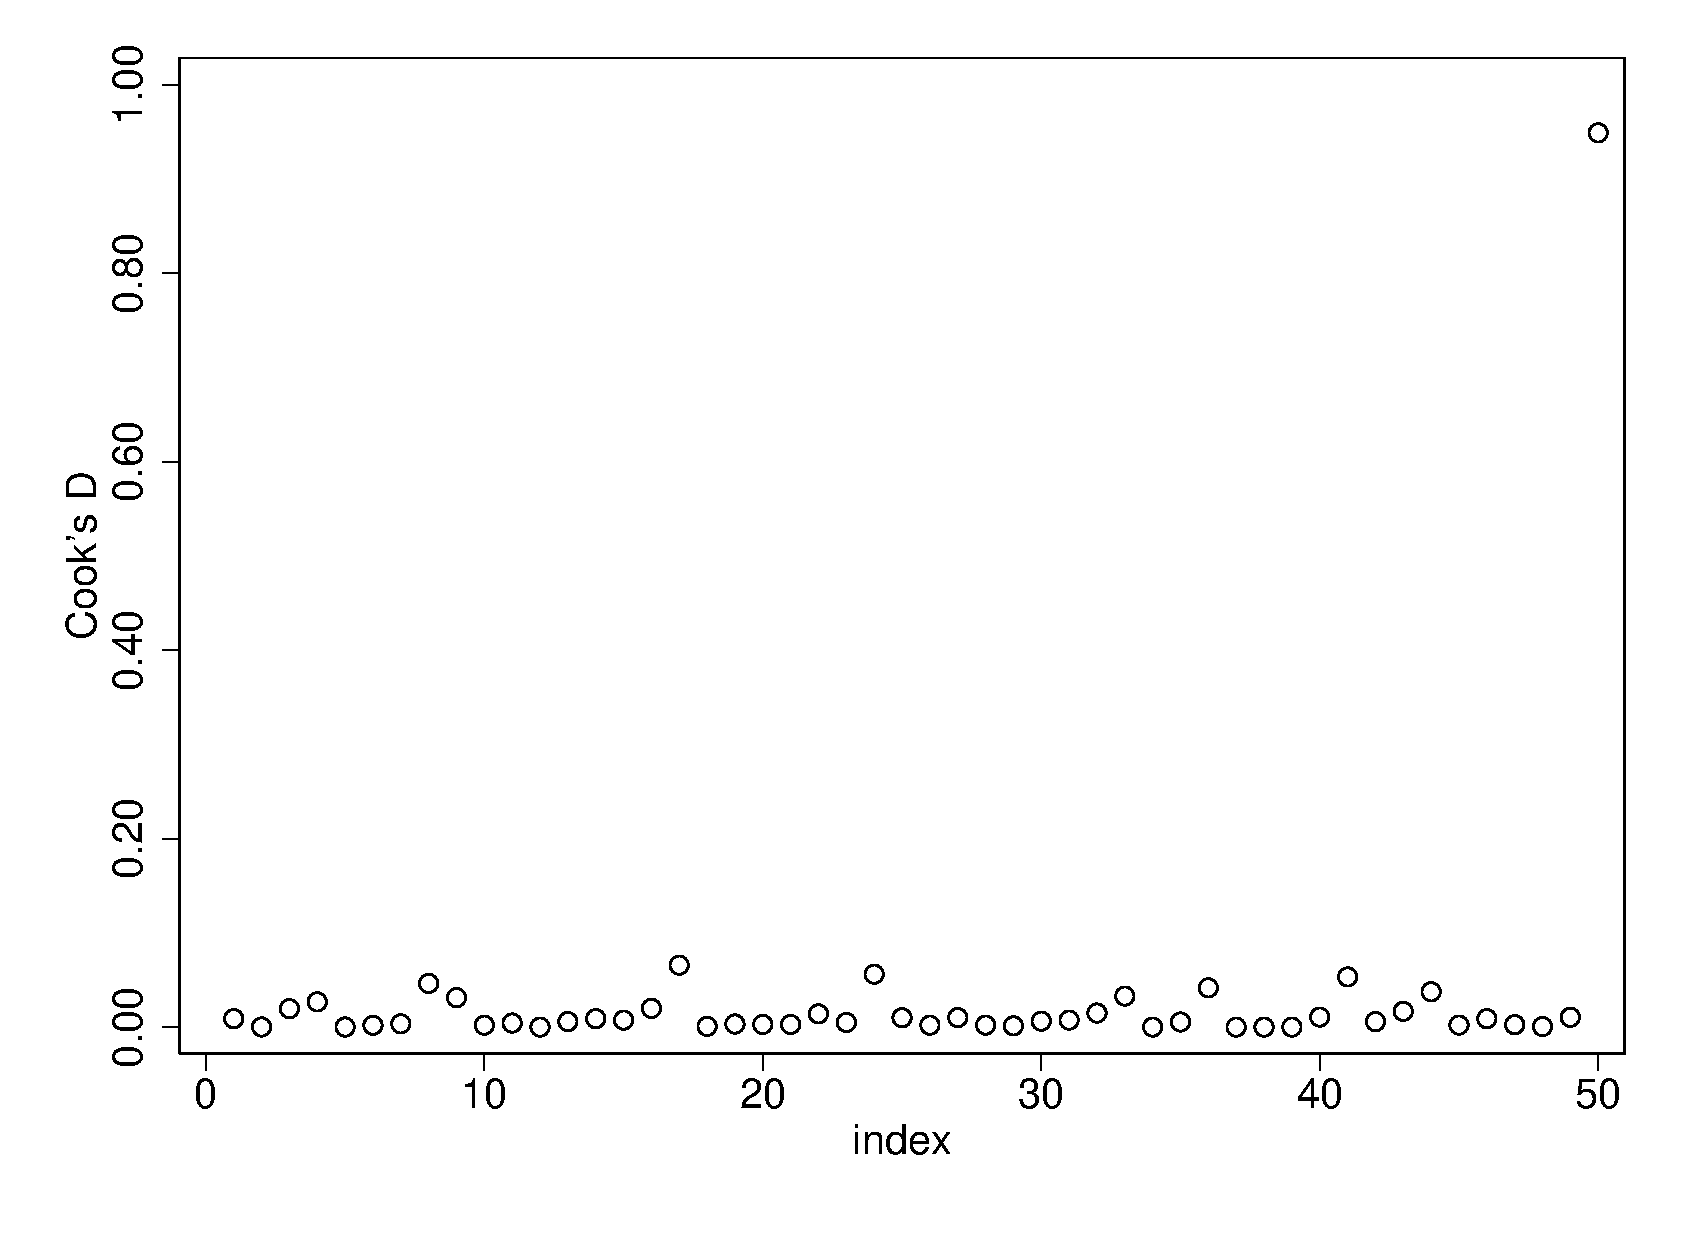
\includegraphics[angle=0,
           width=.75\textwidth]{xout_cooks_index.eps}
   \caption{Cook's distance values for extreme value of $x$ by case number of data in Table~\ref{tab:outdata}}
  \label{fig:xcook}
\end{figure}

\begin{figure}
   \centering
   \includegraphics[angle=0,
           width=.75\textwidth]{yout_cooks_index.eps}
   \caption{Cook's distance values for extreme value of $y$ by case number of data in Table~\ref{tab:outdata}}
  \label{fig:ycook}
\end{figure}

Figures with extraordinary values of $x$ and $y$ are displayed in Figures~\ref{fig:xcook} and ~\ref{fig:ycook}, respectively.

\section{Dfits}


Similar to Cook's distance is the DFITS measure.

\begin{equation}
D_i = e_i\times \sqrt{\frac{h_i}{1-h_i}}
\end{equation}

Figures with extraordinary values of $x$ and $y$ are displayed in Figures~\ref{fig:xdfit} and ~\ref{fig:ydfit}, respectively.

\begin{figure}
   \centering
   \includegraphics[angle=0,
           width=.75\textwidth]{xout_dfit_index.eps}
   \caption{D-fit values for extreme value of $x$ by case number of data in Table~\ref{tab:outdata}}
  \label{fig:xdfit}
\end{figure}

\begin{figure}
   \centering
   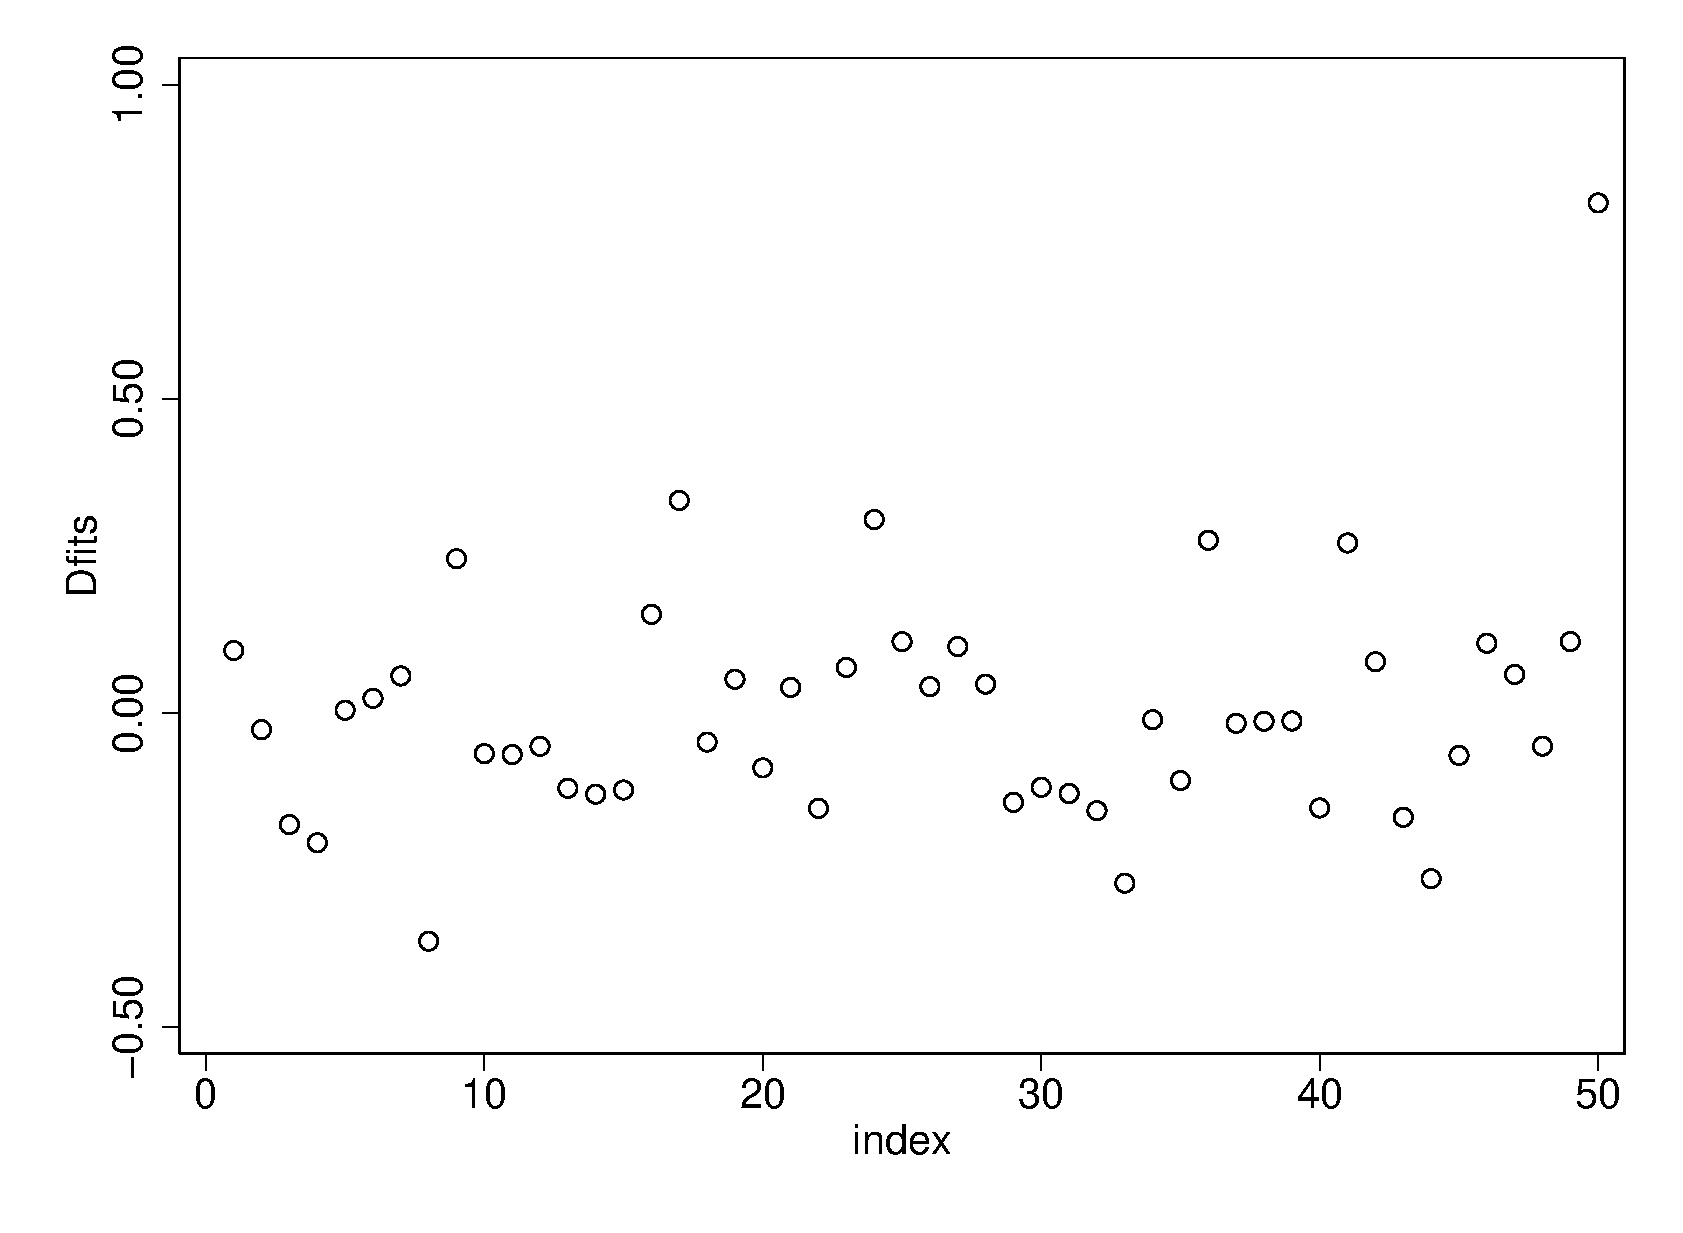
\includegraphics[angle=0,
           width=.75\textwidth]{yout_dfit_index.eps}
   \caption{D-fit values for extreme value of $y$ by case number of data in Table~\ref{tab:outdata}}
  \label{fig:ydfit}
\end{figure}

\section{Summary}

As you can see, there are several measures to detect outliers. In most cases, it will be difficult to spot them initially. Table~\ref{tab:outsum} gives a general summary of the different methods and how well they work to discover extreme $x$ or $y$ values. In the end, I recommend the use of the Dfits measure as it combines the leverage values with the residuals (thus involves both the outcome and predictors).

\begin{table}[htbp]\centering
\caption{Summary of outlier measures for extreme $x$ and $y$
\label{tab:outsum}}
\begin{tabular}{lll}
\hline
Measure & Extreme $x$ & Extreme $y$ \\
\hline
Leverage & Yes & No \\
Standardized residuals & No & Yes \\
Studentized residuals & Maybe & Yes \\
DFBETA & Yes & No \\
Cook's distance & Yes & Maybe \\
DFits & Yes & Yes \\
\hline
\end{tabular}
\end{table}



\chapter{Coding strategies}
This chapter is all about how to alter our predictors and outcomes to make regression models give us the information we need to know.
\section{Centering}
The most basic transformation of a variable is to add or subtract something from it. An important example of this is to center a variable. This is also called de-meaning a variable (but I prefer "centering"). Centering a variable is the simple procedure of taking a variable and subtracting its mean value.
\begin{equation}
x_i^{*}=x_i-\bar{x}
\end{equation}
This does powerful things for regressions and it makes your life easier. The benefits include making your intercept more interpretable and understanding complex coding schemes such as interactions much easier. It should be noted that centering will not change your slopes or the standard errors of your slopes. It will change your intercept and the standard error of your intercept.

It works by moving the $y$-intercept to the mean of your predictor. Since the intercept is always when your predictor(s) are 0, you make 0 the mean when you subtract it, see Figure~\ref{fig:centering_fit}.
\begin{figure}
   \centering
   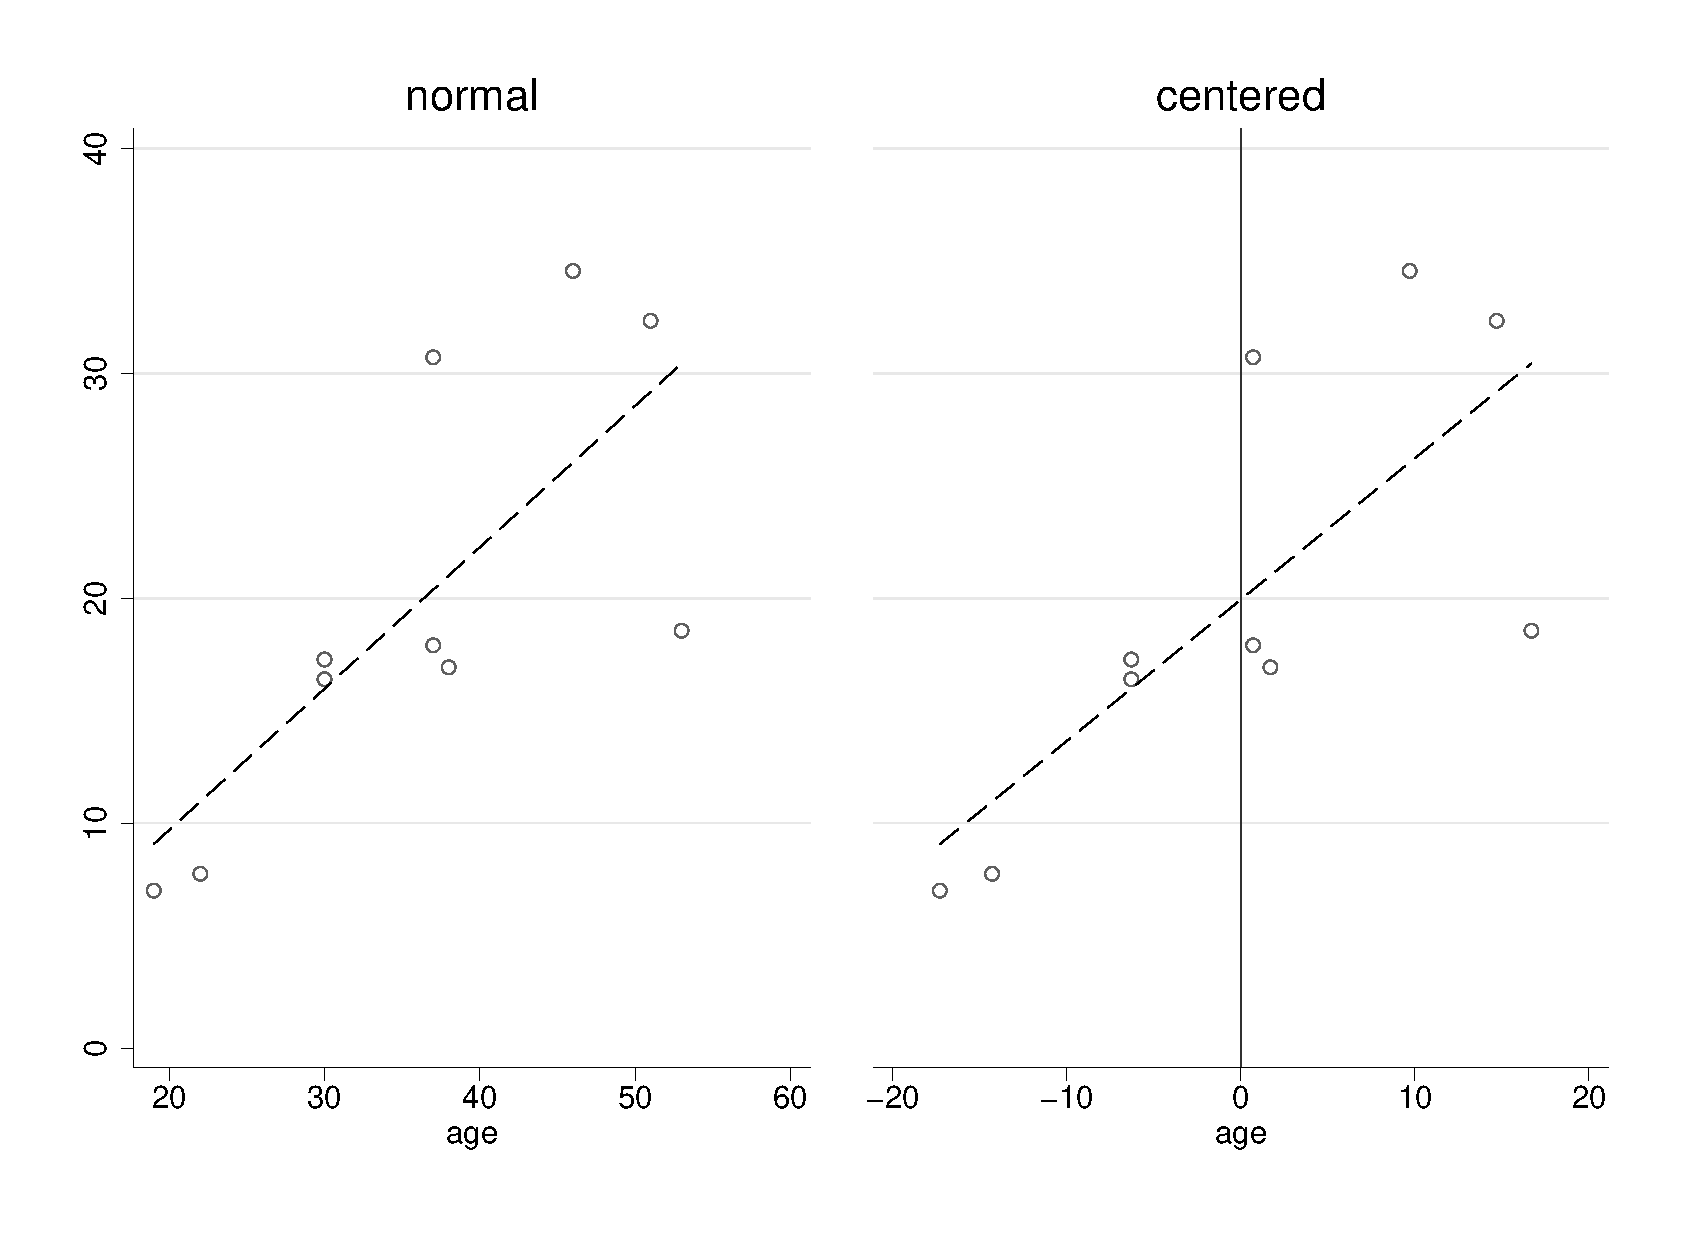
\includegraphics[angle=0,
           width=.75\textwidth]{centering_fit.eps}
   \caption{Illustration of centering}
  \label{fig:centering_fit}
\end{figure}
Centering can be done in models with a single variable or with many variables.

To understand what centering does, consider Model 3 from Table~\ref{tab:wagereg_all}:
\[
\hat{y}_i=\beta_0+\beta_1edu_i+\beta_2age_i+\beta_3female_i
\]
We know that $\beta_1$ is the effect of a single year of education on wages, $\beta_2$ is the effect of a single year of age on wages, and $\beta_3$ is the difference between females and males. What does $\beta_0$ mean again? It's the (average) value of $wage$ when $edu$, $age$, and $female$, all equal zero. Consider the models in Table~\ref{tab:wagecenter}, which use more data than the wage models in the other tables. In Model 1, none of the variables are centered.  So, according to this model, the intercept tells us that uneducated babies who are male make -4.651 dollars an hour. This doesn't make sense on many levels.
\begin{table}[htbp]\centering
\caption{Models predicting age with different centering strategies
\label{tab:wagecenter}}
\begin{tabular}{lccc}
\hline
Coefficients&Model 1&Model 2&Model 3 \\
\hline
edu &    0.930***&    0.930***&    0.930***\\
      &   (0.034)  &   (0.034)  &   (0.034)  \\
age     &    0.261***&    0.261***&    0.261***\\
      &   (0.009)  &   (0.009)  &   (0.009)  \\
female   &   -3.474***&   -3.474***&   -3.474***\\
      &   (0.207)  &   (0.207)  &   (0.207)  \\
Intercept    &   -4.651***&    5.006***&   17.289***\\
      &   (0.597)  &   (0.474)  &   (0.147)  \\
\hline
\multicolumn{4}{l}{Model Statistics} \\
\hline
$N$ 							&  3997.000  &  3997.000  &  3997.000  \\
$F$ 							&   590.668  &   590.668  &   590.668  \\
$R^2$ 						&    0.307  &    0.307  &    0.307  \\
$df$ Regression 			&    3.000  &    3.000  &    3.000  \\
Sum of Squares Regression 	&  75828.174  &  75828.174  &  75828.174  \\
$df$ Error 					&  3993.000  &  3993.000  &  3993.000  \\
Sum of Squares Error 		& 170869.757  & 170869.757  & 170869.757  \\
\hline
\multicolumn{4}{l}{Model 2: age centered, Model 3: edu and age centered.} \\
\multicolumn{4}{l}{$SE$s in parentheses, $***p<0.001$} \\
\hline
\end{tabular}
\end{table}
We now move to Model 2, where we have centered age. Now the intercept tells us that an {\it averaged aged} male with no education can expect to make about 5 dollars an hour. This is plausible. Next, in Model 3, we also center education. Now, an averaged aged male with an average number of years of education makes 17.30 an hour. Notice that in each case, while the intercept changed, the standard error of the intercept kept getting smaller and smaller. No other numbers in the table changed.

The standard error of the intercept gets smaller because the variance of any predicted value is always lowest at the mean. The reason for this is because the variance of any predicted value of $y$ based on some value of $x$, say $x_0$, is equation~\eqref{eq:varfit}
\[
\mbox{var}\left(\hat{y}_0\right)=\left(\frac{\sigma^2}{N}+\frac{\left(x_0-\bar{x}\right)^2\sigma^2}{\sum_{i=1}^N\left(x_i-\bar{x}\right)^2}\right)\sigma^2
\]
and that fraction to the right gets smaller the closer the value is to the mean of $x$. This gets reflected in the smaller standard error of the intercept.
\begin{figure}
   \centering
   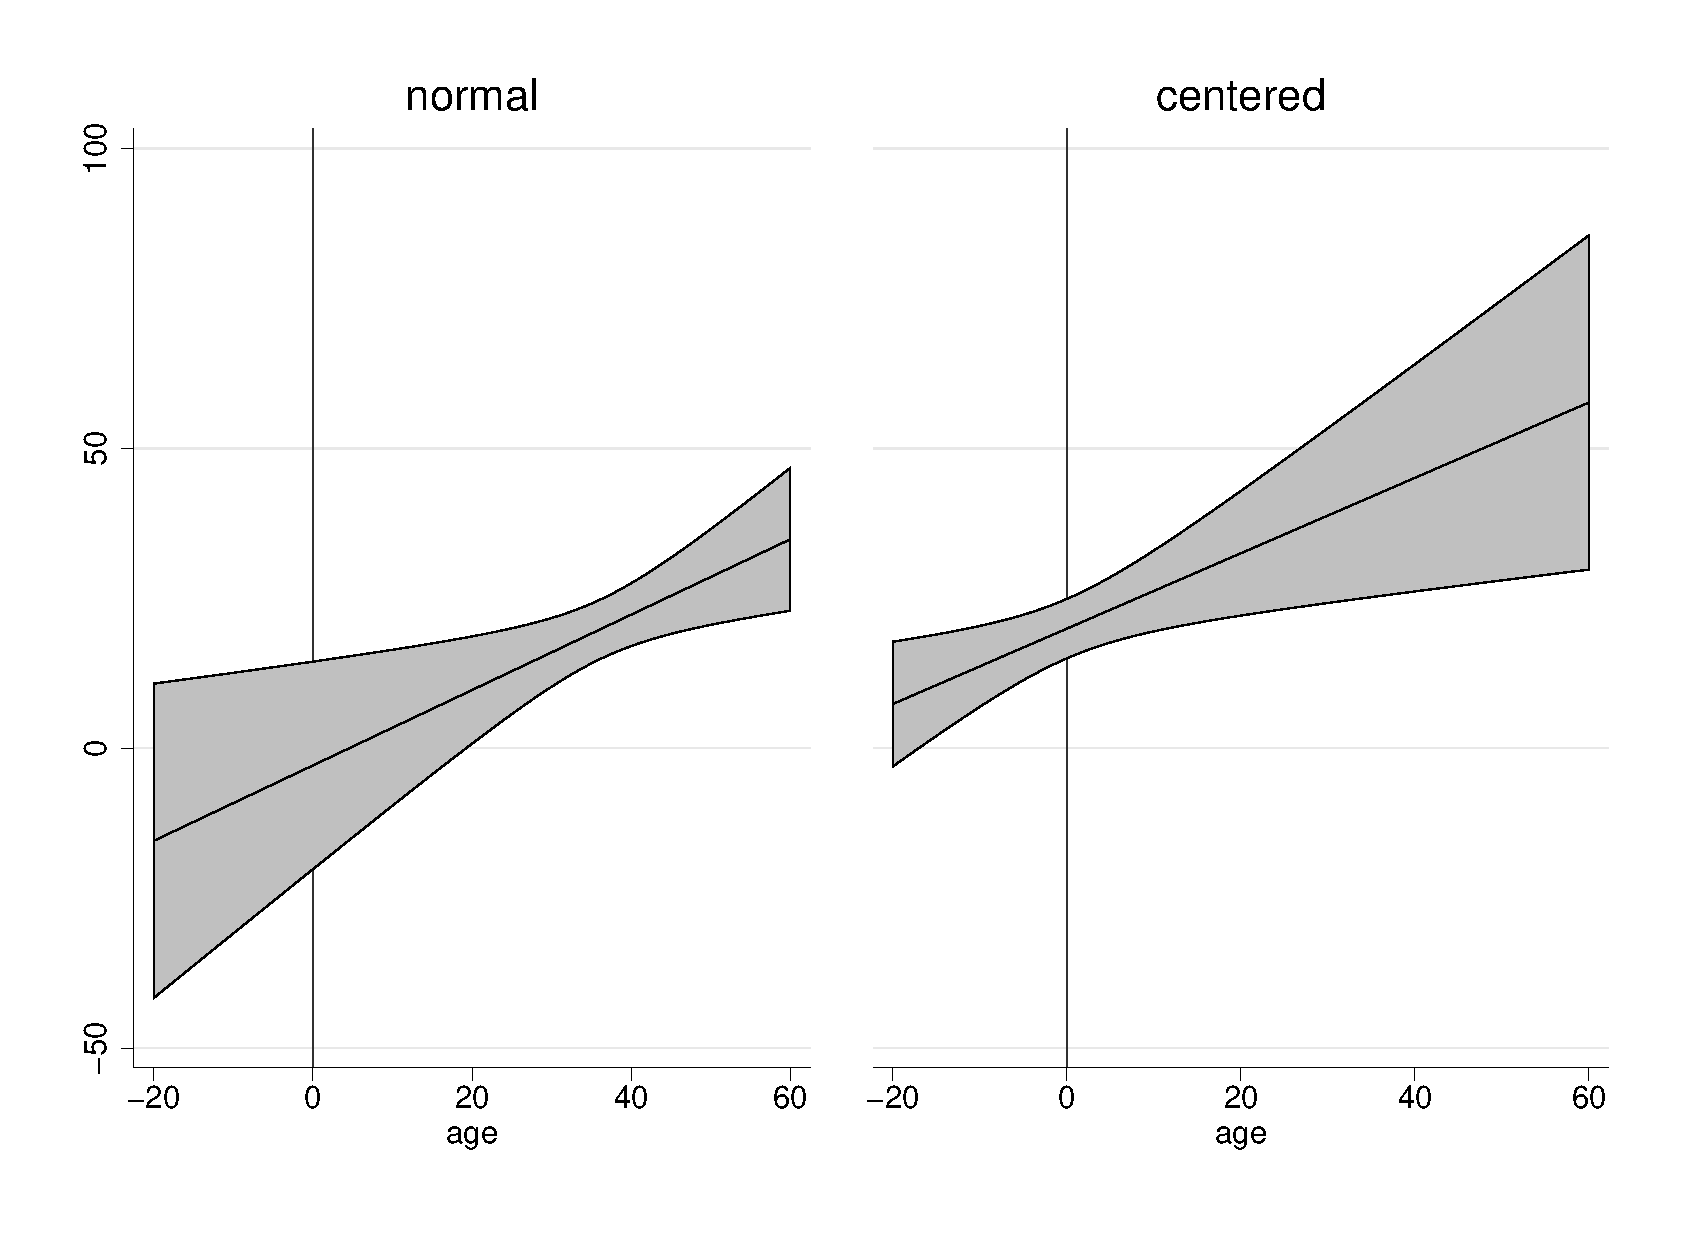
\includegraphics[angle=0,
           width=.75\textwidth]{centering_fitci.eps}
   \caption{Confidence interval of regression line}
  \label{fig:centering_fitci}
\end{figure}
We can see this in the bivariate case by looking at Figure~\ref{fig:centering_fitci}. Note how the confidence intervals are small around the mean of the distribution of the predictor. Centering moves the intercept to this point of small(er) variance. Centering is a good practice for building a good "reference" statistic.

\begin{table}[htbp]\centering
\caption{ Wage models with different age and education units
\label{tab:wagereg_alt}}
\begin{tabular}{lccc}
\hline
Coefficients&Model 1&Model 2&Model 3 \\
\hline
edu &    0.930***&    0.930***&    2.823***\\
      &   (0.034)  &   (0.034)  &   (0.104)  \\
age     &    0.261***&    2.613***&    2.613***\\
      &   (0.009)  &   (0.087)  &   (0.087)  \\
female   &   -3.474***&   -3.474***&   -3.474***\\
      &   (0.207)  &   (0.207)  &   (0.207)  \\
Intercept    &   -4.651***&   -4.651***&    7.632***\\
      &   (0.597)  &   (0.597)  &   (0.353)  \\
\hline
\multicolumn{4}{l}{Model Statistics} \\
\hline
$N$ &  3997.000  &  3997.000  &  3997.000  \\
$F$ &   590.668  &   590.668  &   590.668  \\
$R^2$ &    0.307  &    0.307  &    0.307  \\
$df$ Regression &    3.000  &    3.000  &    3.000  \\
Sum of Squares Regression 	 &  75828.174  &  75828.174  &  75828.174  \\
$df$ Error 		 &  3993.000  &  3993.000  &  3993.000  \\
Sum of Squares Error 	 & 170869.757  & 170869.757  & 170869.757  \\
\hline
\multicolumn{4}{l}{Model 2: age in 10 year units.} \\
\multicolumn{4}{l}{Model 3: age in 10 year units and edu is standardized.} \\
\multicolumn{4}{l}{$SE$s in parentheses, $***p<0.001$} \\
\hline
\end{tabular}
\end{table}

\section{Changing the unit}

A regression slope always tells us the difference in the outcome based on a single-unit increase in the predictor. Sometimes, a single unit increase isn't meaningful. For example, take age. Your wage probably won't increase that much from year to year. According to Table~\ref{tab:wagecenter}, Model 1, it will increase by 26.1 cents a year. A more meaningful distinction would be 10 years of age.

To capture this, we could divide age by 10 and rerun the model. This would make $\beta_2=2.613$. By moving the decimal of the predictor left, we move the decimal of the slope (and standard error) to the right. Compare the effect of age in Models 1 and 2 in Table~\ref{tab:wagereg_alt}. Nothing else changes. It is good practice to keep your predictors in units to maximize the digits available in your tables.

\section{Standardization}

Another transformation is $z$-scoring. It is simply centering the predictor and dividing by the standard deviation of the predictor
\begin{equation}
x_i^{(z)}=\frac{x_i-\bar{x}}{s_x}
\end{equation}

Sometimes this is called standardization. This changes the units of the variable into "standard deviation" units. This also centers variables on their mean. The slope's interpretation is now that a one-unit increase in the predictor is "a standard deviation" increase. Compare the effect of education in Models 2 and 3 in Table~\ref{tab:wagereg_alt}. In Model 2, for every year of education, wages increase by 93 cents. In Model 3, we see that an increase of a standard deviation in education increases wages by about 2.82 dollars. Nothing else changes.


\section{Power Transformations}

Sometimes the data are not linear. They need to be linear for a regression to count. There are several ways to transform data. One is the Box-Cox family of transformations
\begin{equation}
x\rightarrow x^p\equiv\frac{x^p-1}{p}\forall p>0
\end{equation}
This gives us the various effects of squaring, etc. This is nice when we think that the effect of $x$ on $y$ is not constant (like it accelerates or decelerates). {\bf Be careful with squares, always graph out our predicted values to know what you are dealing with}.

Many people make the mistake that just because a square term is significant, it must mean a u-shaped relationship. That depends on the strength of the main effect (i.e., the effect of $x$) and the effect of the square (i.e., the effect of $x^2$). Figures~\ref{fig:square1} through~\ref{fig:square4} illustrate the differences.
\begin{figure}
   \centering
   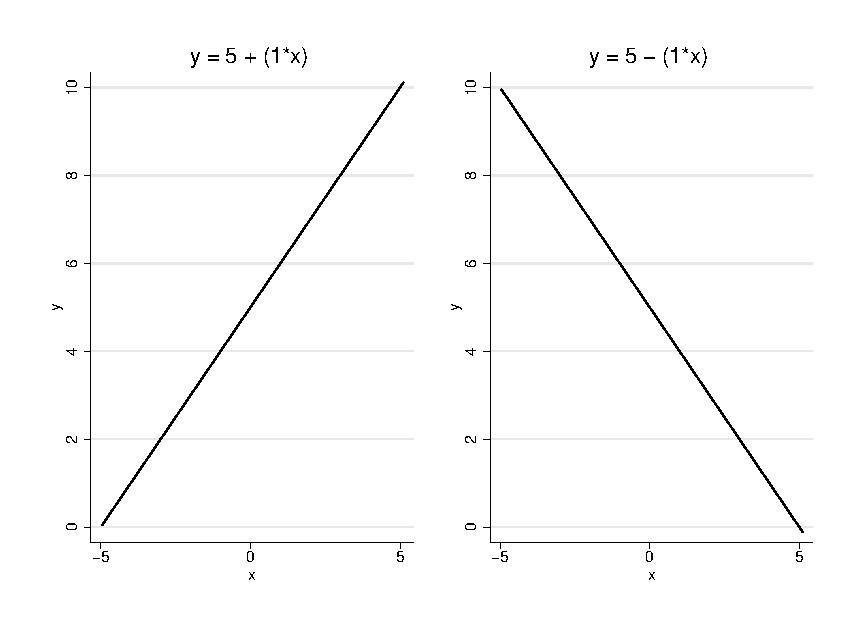
\includegraphics[angle=0,
           width=.75\textwidth]{square1.eps}
   \caption{Models without a quadratic relationships}
  \label{fig:square1}
\end{figure}
\begin{figure}
   \centering
   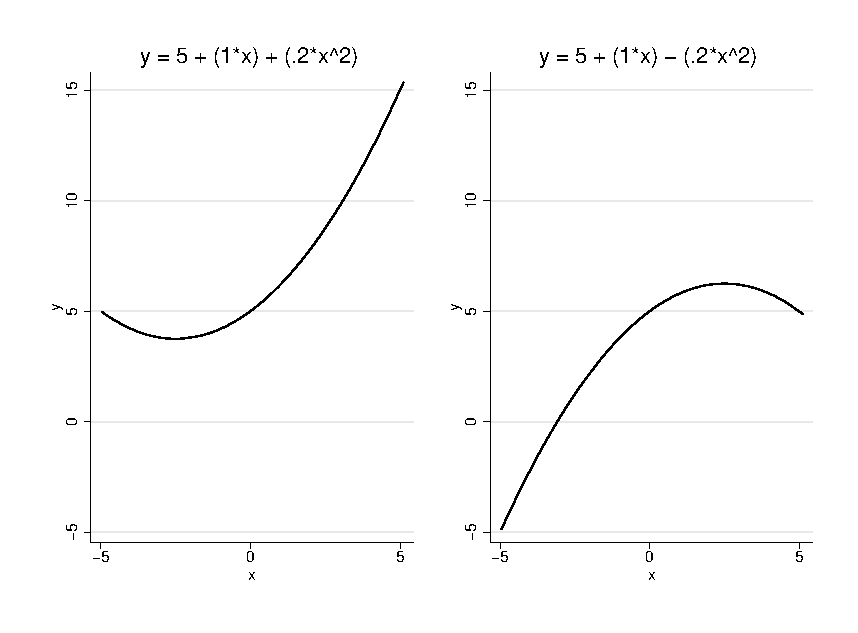
\includegraphics[angle=0,
           width=.75\textwidth]{square2.eps}
   \caption{Models with a positive relationship that accelerates (left) and one that decelerates (right)}
  \label{fig:square2}
\end{figure}
\begin{figure}
   \centering
   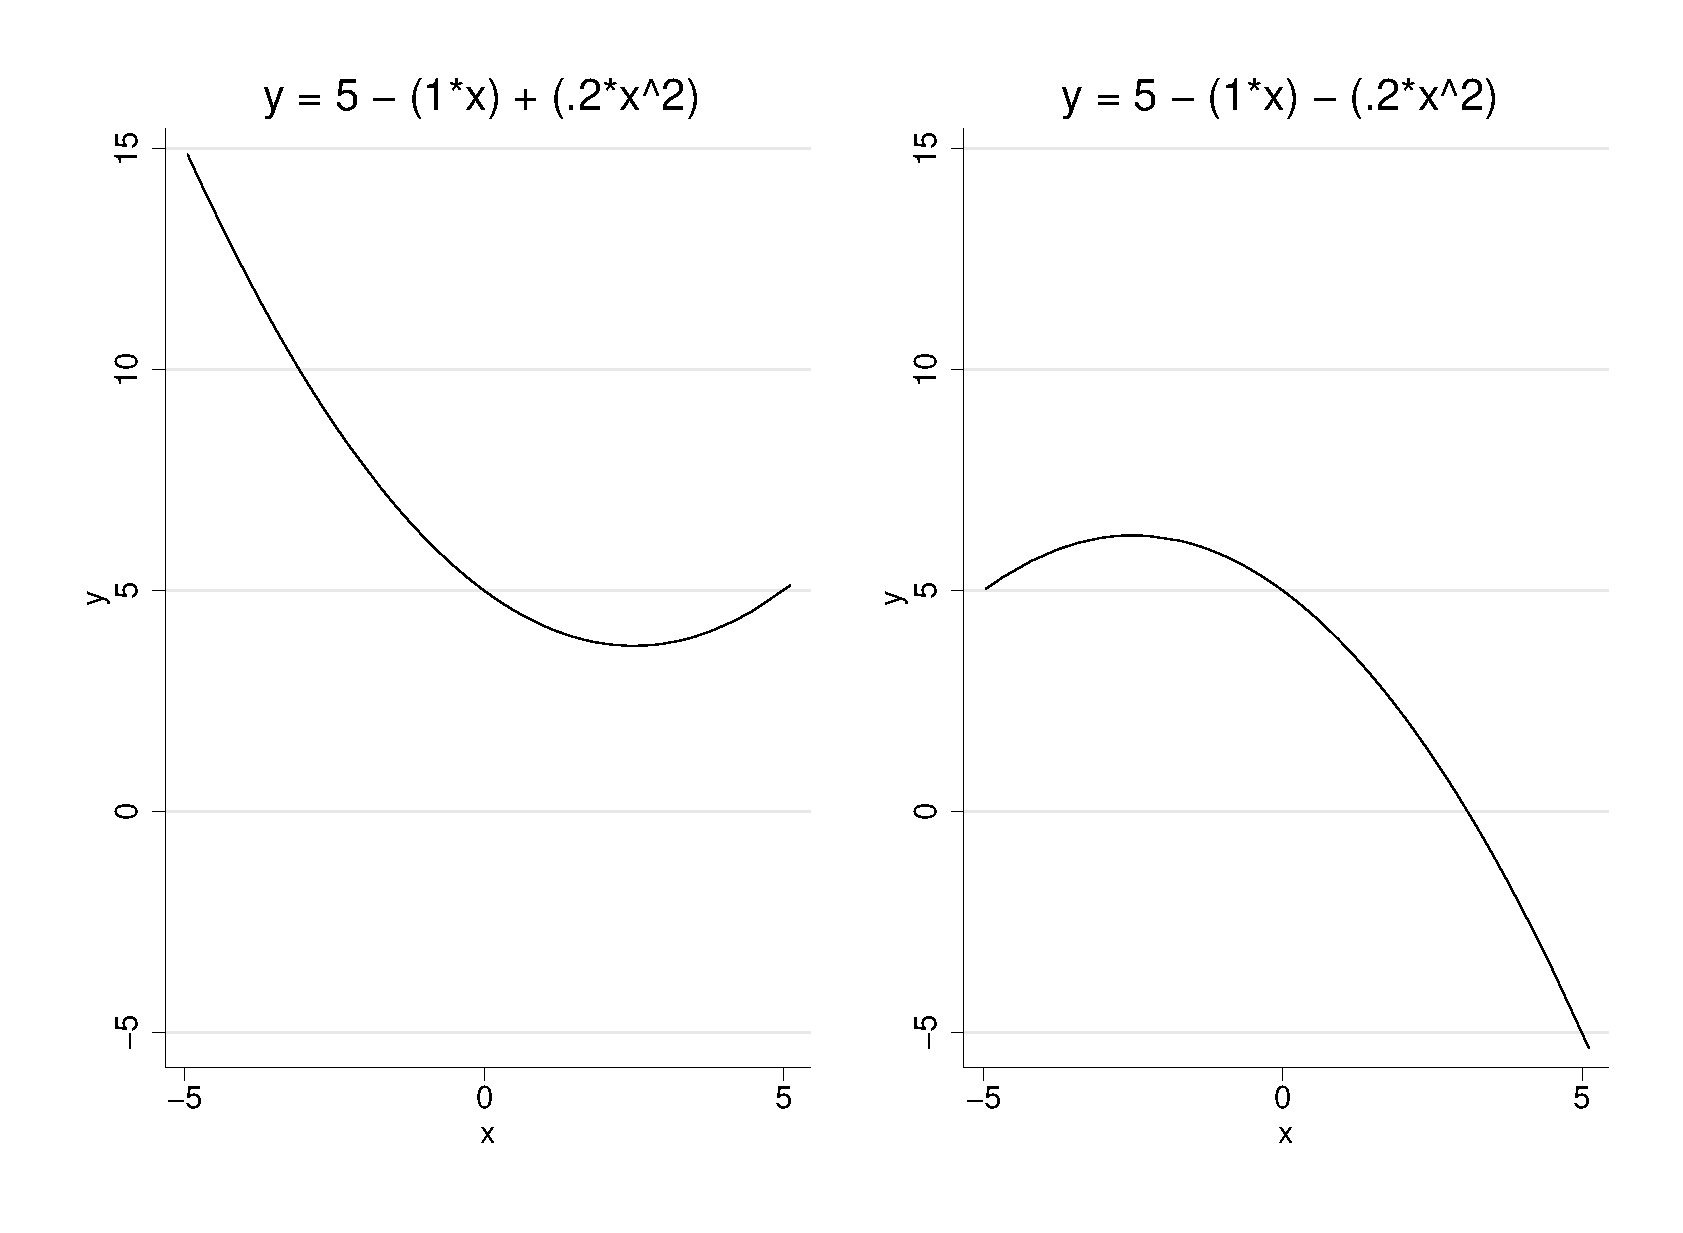
\includegraphics[angle=0,
           width=.75\textwidth]{square3.eps}
   \caption{Models with a negative relationship that decelerates (left) and one that accelerates (right)}
  \label{fig:square3}
\end{figure}
\begin{figure}
   \centering
   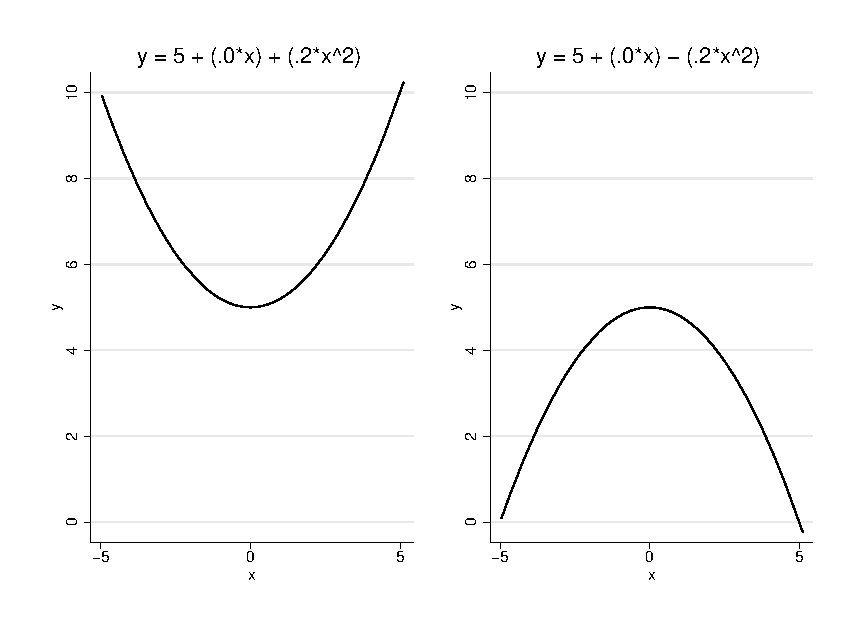
\includegraphics[angle=0,
           width=.75\textwidth]{square4.eps}
   \caption{Models without a main effect but a positive quadratic relationship (left) and a negative relationship (right)}
  \label{fig:square4}
\end{figure}
What can also be important is to know what the slope of the line is at any given point along the line. Let's take the function
\[
y=\beta_0-\beta_1x-\beta_2x^2
\]
\[
y=5-1x-0.2x^2
\]
What is the slope (or the slope of the tangent line) of this line at $x = 0.50$? Calculus gives us an easy formula for this
\begin{equation}
\frac{\partial y}{\partial x}|x=\beta_1+2\beta_2x
\end{equation}
for example, when x = 0.50,
\[
\frac{\partial y}{\partial x}|x=-1+2\left(-.2\right)x
\]
\[
\frac{\partial y}{\partial x}|x=-1+2\left(-.2\right)0.50
\]
\[
\frac{\partial y}{\partial x}|x=-1.2
\]
This is visualized in Figure~\ref{fig:calc}; notice the intercept for the tangent line is the same as the regression line.
\begin{figure}
   \centering
   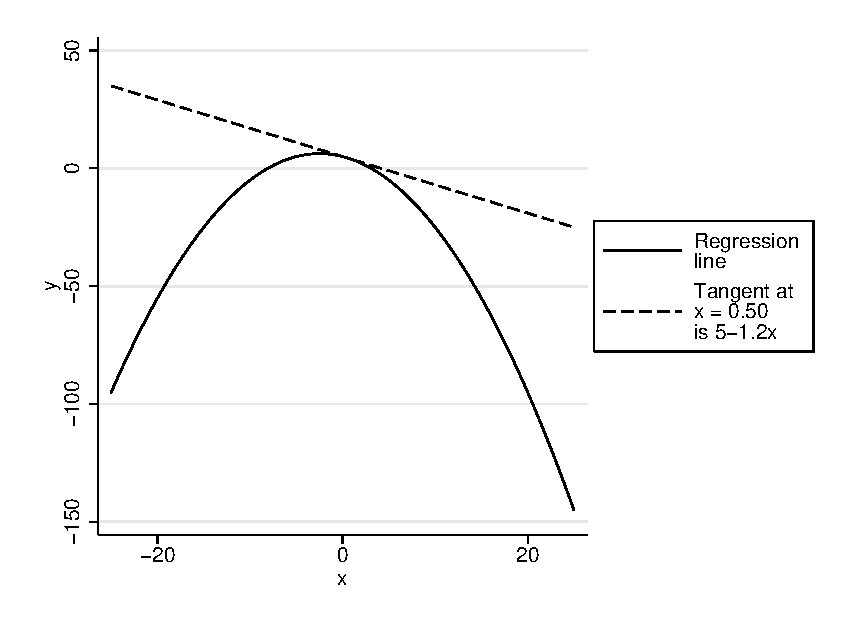
\includegraphics[angle=0,
           width=.75\textwidth]{calc.eps}
   \caption{Quadratic relationship with tangent}
  \label{fig:calc}
\end{figure}
\subsection{Logs}
\label{sec:logs}
A special case of a power transformation is the log. Figure~\ref{fig:ln} shows the natural log, $\mbox{ln}\left(x\right)$.
\begin{figure}
   \centering
   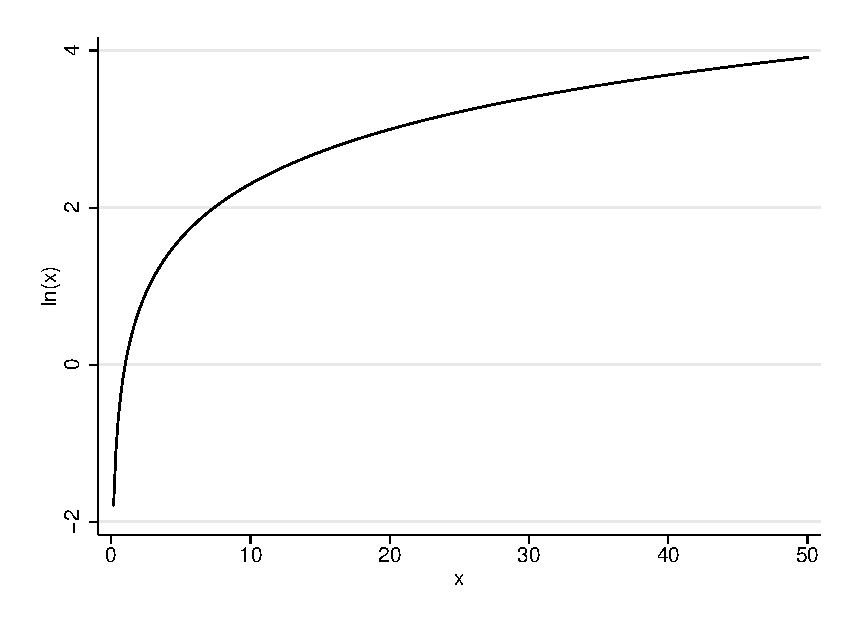
\includegraphics[angle=0,
           width=.75\textwidth]{ln.eps}
   \caption{ln($x$)}
  \label{fig:ln}
\end{figure}
This helps tone down predictors, and even outcomes, that are highly skewed. Once transformed, we can then run our regression on them. Even more fun is logging both $x$ and $y$, which produces an elasticity (i.e., a 1 percent increase in $x$ gives a $\beta$ percent change in $y$).
\subsubsection{Examples with logs as outcome, predictor, or both}
\label{sec:midpointref}
I have a sample of people who give to charities. We want to know the relationship between what they give and their income in thousand dollar units. Table~\ref{tab:charitydes} give the summary statistics of the variables we will use: the amount given to charity in the last year, household income in thousand dollar units\footnote{In this section we present data where income was measured as several categories and total amount given was assessed numerically. We transform the income categories into the midpoint dollar amount, then divide by 1000.}, the natural log of the amount given, and the natural log of the household income in thousands.
\begin{figure}
   \centering
   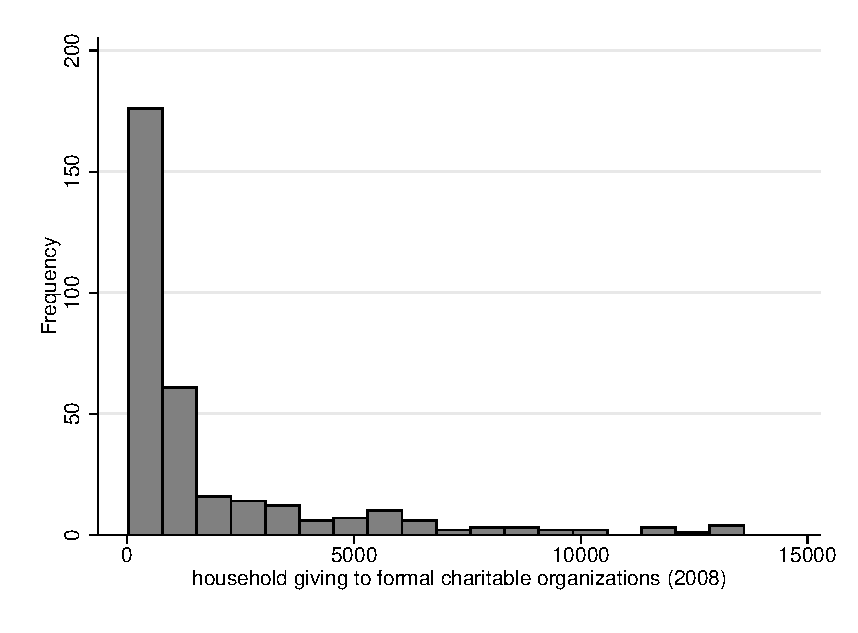
\includegraphics[angle=0,
           width=.75\textwidth]{gave.eps}
   \caption{Distribution of charitable giving}
  \label{fig:gave}
\end{figure}
\begin{table}[htbp]
\caption{\label{tab:charitydes} Summary statistics for charity models}\centering\medskip
\begin{tabular}{llcc}\hline
Variable & Description & $mean$ & $SE\left(mean\right)$  \\ \hline
gaveamt & Amount given & 1796.99 & 148.64 \\
hhincome & Income in k & 60.36 & 1.20 \\
lngaveamt & ln(Amount given) & 6.54 & 0.08 \\
lnhhincome & ln(Income in k) & 4.02 & 0.02 \\ \hline
 \end{tabular}
\end{table}
When we examine our outcome, amount given, we see that it is highly skewed, see Figure~\ref{fig:gave}. This will most likely produce several problems:
\begin{enumerate}
\item The variance will not be constant
\item The mean of the residuals will not consistently be zero
\item We may have outliers in the tail of the distribution
\end{enumerate}


\begin{table}[htbp]\centering
\caption{ Models predicting charitable giving in dollars
\label{tab:charity}}
\begin{tabular}{lcccc}
\hline
Coefficients&Model 1&Model 2&Model 3&Model 4 \\ \hline
hhincome centered  &   22.614*** &    0.014*** &        &        \\
      &   (6.777)  &   (0.004)  &        &        \\
ln(hhincome) centered &        &        &  1156.648** &    0.730*** \\
      &        &        &  (356.840)  &   (0.193)  \\
Intercept    &  1796.988*** &    6.543*** &  1796.988*** &    6.543*** \\
      &  (146.392)  &   (0.079)  &  (146.528)  &   (0.079)  \\
\hline
\multicolumn{5}{l}{Model Statistics} \\
\hline
$N$ &   328.000  &   328.000  &   328.000  &   328.000  \\
$F$ 	 &   11.134  &   14.822  &   10.506  &   14.296  \\
$R^2$  &    0.033  &    0.043  &    0.031  &    0.042  \\
$df$ Regression &    1.000  &    1.000  &    1.000  &    1.000  \\
$df$ Error 		 &   326.000  &   326.000  &   326.000  &   326.000  \\
Log-likelihood &  -3049.966  &  -582.776  &  -3050.271  &  -583.030  \\
\hline
\multicolumn{5}{l}{Models 2 and 4 have a logged outcome. hhincome in thousand dollar units.} \\
\multicolumn{5}{l}{$SE$s in parentheses, $***p<0.001$} \\
\hline
\end{tabular}
\end{table}
Table~\ref{tab:charity} presents four models. The first model predicts giving with income using the unaltered versions of both variables (note: income is centered):
\[
gave_i=\beta_0+\beta_1\left(hhincome_i-\overline{hhincome}_i\right) + e_i.
\]
The second model predicts the natural log of giving with the unaltered version of income:
\[
\mbox{ln}\left(gave_i\right)=\beta_0+\beta_1\left(hhincome_i-\overline{hhincome}_i\right)+e_1.
\]
The third model predicts unaltered giving with the natural log of income, centered on the mean natural log of income:
\[
gave_i=\beta_0+\beta_1\left(\mbox{ln}\left(hhincome\right)_i-\overline{\mbox{ln}\left(hhincome\right)}_i\right) + e_i.
\]
Finally, the fourth model predicts the natural log of giving with the natural log of income, centered as well:
\[
\mbox{ln}\left(gave_i\right)=\beta_0+\beta_1\left(\mbox{ln}\left(hhincome\right)_i-\overline{\mbox{ln}\left(hhincome\right)}_i\right)+e_i.
\]
\paragraph{Interpretation of Model 1}

Since we centered income, the intercept indicates that a household with average income gives about 1,797 dollars. For each thousand dollars increase in income, giving increases by about 23 dollars. Overall, this model explains about 3.3 percent of the variation.

\paragraph{Interpretation of Model 2}

In this model, we have transformed giving into the natural log of giving. Income is still centered, so the intercept is still the average natural log of giving. We can take the exponent of this quantity to estimate the geometric mean of giving (not the arithmetic mean)
\begin{equation}
e^{\beta_0} = \left(\bar{y}_{geometric}|x=0\right)
\end{equation}
\[
e^{6.543} = 694.37
\]
which tells us that the average household gives about 694 dollars. This estimate is much smaller than Model 1 (1,797 dollars).

Estimating the effect of income requires us to take the exponent of $\beta_1$. Thus, $\left(e^{\beta_1}-1\right)\times100$ will tell us the percent increase in the outcome for a one unit change in the predictor if $\beta_1>0$. When $\beta_1<0$, $\left(1-e^{\beta_1}\right)\times100$ will tell us the percent decrease in the outcome for a one unit change in the predictor. For example, when income is at the mean, we have already established that the amount given is 694.37 dollars. If we increase income by a thousand dollars (a one unit increase), the dollar amount given is
\[
e^{6.543+0.014} = 704.16
\]
The ratio of these two amounts is
\[
\frac{y|x=1}{y|x=0} = \frac{704.16}{694.37}=1.014
\]
which is equal to the exponent of the slope
\[
e^{\beta_1}=\frac{y|x=1}{y|x=0}
\]
\[
e^{0.014}=1.014
\]
which indicates a
\[
\left(e^{\beta_1}-1\right)\times100 = \left(1.014-1\right)\times100=1.4 \mbox{ percent}
\]
increase. Note that the fact that the coefficient was 0.014 and the percent increase was 1.4 is a coincidence. When the coefficient is larger, the numbers will not match.

If we log these variables, their distributions behave better (but what we really care about is the distribution of giving)

\paragraph{Interpretation of Model 3}

We know that the average donation for the log of the average household income is 1,796.99. What does the coefficient mean? To understand that we need to realize that since we logged our predictor, our comparison is between the average log and an additional log. This would be a lot of income. Let's instead say that income increases 10 percent (or by a factor of 1.1). This makes the difference in our outcome as
\[
1156.648\times\mbox{ln}\left(1.1\right)=110.24 \mbox{ dollars}
\]

The final use of log-transformations in OLS regression is when both dependent and predictor variable are logged.

\paragraph{Interpretation of Model 4}

In this model, both the outcome and predictor is transformed to the natural log. This produces an elasticity. Thus, coefficient tells us the percent ({\it not proportion}) change in the outcome based on a 1 {\it percent} change in the predictor. Here, we see that giving changes by 0.730 percent, for each percentage change in the predictor. Here is a walk-through on how this works.

Table~\ref{tab:charitydes} gives the means for our variables, both the unaltered version and the natural log version. From Table~\ref{tab:charity}, we can find that the dollar amount for the mean natural log of giving is $e^{6.543}=694.37$ dollars. The mean natural log of income is 4.02, which translates into an amount of $e^{4.02}=55.70$ thousand dollars. A 1 percent increase of 55.70 thousand dollars is $1.01\times55.70 = 56.26$ thousand dollars, of which the natural log is 4.03. Thus, a 1 percent increase in the natural log of income is 0.01. Plugging this into the model, our predicted natural log of giving is $6.543+0.730\left(0.01\right)=6.550$, the exponent of which is 699.45. $\left(699.45 - 694.37\right)/694.37=0.01$, or a 1 percent increase.

\subsubsection{Testing models with log likelihoods}
\label{sec:likelihoodtest}
As a bonus, Table~\ref{tab:charity} includes the log likelihood of each model. We can only compare log likelihoods for models with the same outcome and exact same set of data. That means we can compare Models 1 and 3, and Models 2 and 4.

Recall that the log likelihood of a model is $\mbox{ln}\left(L\left(\theta\right)\right)$. Also remember that the test of two log likelihoods for models A and B is equation~\eqref{eq:lrtest}
\[
\chi^2=2\left(\mbox{ln}\left(L\left(\theta_a\right)\right)-\mbox{ln}\left(L\left(\theta_{null}\right)\right)\right)
\]
We see the log likelihood of Model 1 in Table~\ref{tab:charity}, the model with unaltered predictors with the unaltered outcome, is -3029.966, and the likelihood of Model 3, the model with the natural log of income with the unaltered outcome is -3050.271. The test comparing whether Model 3 is a better model is
\[
\chi^2=2\left(-3029.966- -3050.271\right)=40.61
\]
We can then evaluate this against the $\chi^2$ distribution with 1 degree of freedom, which produces a probability of 0.000000002. This is clear evidence that using the unaltered version of the predictor, Model 1, is a much better model. Looking at Models 2 and 4, this test results in 0.508, the probability of which is 0.476, telling us that there is no difference, statistically, in the model fit between Models 2 and 4.

\section*{For more information}
For comprehensive treatment of variable coding and transformation strategies in regression, see \citep{fox} and \citep{hill}. For discussion of logarithmic transformations and elasticity interpretations, consult \citep{cameron2005microeconometrics}. Maximum likelihood methods and likelihood ratio testing are covered in detail in \citep{eliason1993maximum}.



\chapter{Analysis of covariance (ANCOVA)}

Analysis of covariance (ANCOVA) is simply a regression with both continuous and categorical predictors. It has, however, a special application in situations in which we have "pre" and "post" scores.

\section{The meaning of the intercept}

Before we enter a categorical predictor, let us first examine some properties of the intercept in models with paired $y$ and $x$ variables. Consider the hypothetical data in Table~\ref{tab:prepostdata}. This table has three columns, the first column is our post-test scores, the second column is our pretest scores, and the third column is the difference for reference. Since the "pre" and "post" tests are from the same units, we can compare the average change with a {\it paired} $t$-test
\begin{equation}
t=\frac{\bar{d}\sqrt{N}}{s_{d}}
\end{equation}
where $\bar{d}$ is the average difference (that is, the average of a new variable measuring the difference) and $s_{d}$ is the standard deviation of those differences. The result for the data in Table~\ref{tab:prepostdata} is $\bar{d}=9.4791$ and $s_{d} = 10.98465$ with 100 observations (which means the standard error of the difference is $\frac{s_{d}}{\sqrt{100}}=1.098465$). This leads to a $t$-value of 8.6294, which has a very small $p$-value.

How can we replicate this result with regression?

\subsection{As-is regression}

The idea is simple, suppose that there was no change, a scatter plot would simply be a diagonal line, as in Figure~\ref{fig:prepostsame}. If, however, on average respondents did change, then the line should rise or fall and this would be reflected in the intercept.

Thus, we may think we could fit the model
\begin{equation}
post_i = \beta_0 + \beta_1 pre_i + e_i
\end{equation}

and look at the intercept.

\begin{figure}
   \centering
   \includegraphics[angle=0,
           width=.75\textwidth]{prepostsame.eps}
   \caption{Scatter plot of data in which pre and post scores are the same with solid regression line}
  \label{fig:prepostsame}
\end{figure}

This thinking is adequate when the regression slope ($\beta_1$) for pre is approximately 1. However, the intercept is less telling about the change for the average pre score if the slope is greater or less than 1, as can be seen in Figure~\ref{fig:prepostalt}

\begin{figure}
   \centering
   \includegraphics[angle=0,
           width=.75\textwidth]{prepostalt.eps}
   \caption{Different functions for pre-post regressions}
  \label{fig:prepostalt}
\end{figure}

A regression of post on pre, however, gives the difference for a low-scoring pre. This is reflected in Model 1 in Table~\ref{tab:prepostreg}, where the intercept is -12.498. This result is very different than the result of the paired $t$-test. The problem is that we are generally interested in the change for the {\it average} pretest, and the intercept reflects the change for a pre of 0.

\subsection{Regression on pre-centered variables}

If we center post and pre, on the {\it pre} mean,
\begin{equation}
post_i-\bar{pre} = \beta_0+\beta_1\left(pre_i-\bar{pre}\right)
\end{equation}
the intercept now reflects the average change for the average pre-test. This is reflected in Model 2 in Table~\ref{tab:prepostreg}. Note that in this case, $\beta_0$ is the result of the paired $t$-test. We can see the difference in Figure~\ref{fig:prepostreg}. When the data are not centered, the intercept is negative. However, by centering both the post and pre on the pre mean, we move the axis for $x$ and $y$ and now the intercept is positive. In general, this gives the {\it average} change for the {\it average} pre, which reflects the paired $t$-test difference.

\begin{figure}
   \centering
   \includegraphics[angle=0,
           width=.75\textwidth]{prepostreg.eps}
   \caption{Scatter plot of data in Table~\ref{tab:prepostdata} with solid regression line and dashed reference lines}
  \label{fig:prepostreg}
\end{figure}

\subsection{Regression on the difference}

The first is to create a new variable that is the difference of post-pre and run an intercept only regression
\begin{equation}
post_i - pre_i = \beta_0 + e_i
\end{equation}
This is represented in Model 3 in Table~\ref{tab:prepostreg}, which reflects the result of the paired $t$-test.

\subsection{Why different standard errors for centered and difference models?}

Comparing Models 2 and 3 in Table~\ref{tab:prepostreg} you will notice that the standard errors for the intercept are different. To understand why, we need to remember where the standard error of intercepts comes from. The intercept is a predicted value (when $x$ is 0), and so like any other predicted value, the variance of the predicted value is equation~\eqref{eq:varfit}
\[
\mbox{var}\left(\hat{y}_0\right)=\left(\frac{\sigma^2}{N}+\frac{\left(x_0-\bar{x}\right)^2\sigma^2}{\sum_{i=1}^N\left(x_i-\bar{x}\right)^2}\right)\sigma^2
\]
and the standard error is
\begin{equation}
\mbox{SE}\left(\hat{y}_0\right)=\sigma\left(\frac{1}{N}+\frac{\left(x_0-\bar{x}\right)^2}{\sum_{i=1}^N\left(x_i-\bar{x}\right)^2}\right)^{1/2}
\end{equation}
which is governed by the residual variation $\sigma$ and the deviation from the mean. In the case of a centered model, the term $\frac{\left(x_0-\bar{x}\right)^2}{\sum_{i=1}^N\left(x_i-\bar{x}\right)^2}$ drops out, which leaves
\begin{equation}
\mbox{SE}\left(\hat{y}_0\right)^{centered}=\sigma\left(\frac{1}{N}\right)^{1/2}
\end{equation}
\begin{equation}
\mbox{SE}\left(\hat{y}_0\right)^{centered}=\frac{\sigma}{\sqrt{N}}
\end{equation}
which is the same as the variance of the mean, c.f. equation~\eqref{eq:meanvar}, and since $\sigma$ is smaller in Model 2 than in Model 3 (because we use the covariate), the standard error is smaller reflecting the use of more information.

\begin{table}[htbp]\centering
 \caption{Models to analyze differences between pre and post data in Table~\ref{tab:prepostdata}
\label{tab:prepostreg}}
\begin{tabular}{lccc}
\hline
Coefficients & Model 1 & Model 2 & Model 3 \\
\hline
Pre      &    1.455***&    1.455***&        \\
      &   (0.102)  &   (0.102)  &        \\
Intercept    &   -12.498* &    9.479***&    9.479***\\
      &   (5.035)  &   (1.007)  &   (1.098)  \\
\hline
\multicolumn{4}{l}{Model Statistics} \\
\hline
N      &   100.000  &   100.000  &   100.000  \\
F      &   202.700  &   202.700  &    0.000  \\
$R^2$     &    0.674  &    0.674  &    0.000  \\
$df$ Regression    &    1.000  &    1.000  &    0.000  \\
Sum of Squares Regression    &  20547.835  &  20547.835  &    0.000  \\
$df$ Error    &   98.000  &   98.000  &   99.000  \\
Sum of Squares Error     &  9934.307  &  9934.307  &  11945.602  \\
$\sigma$    &   10.068  &   10.068  &   10.985  \\
\hline
\multicolumn{4}{l}{Model 2 pre and post both centered on pretest mean} \\
\multicolumn{4}{l}{Model 3 predicts post-pre difference} \\
\multicolumn{4}{l}{$SE$s in parentheses, $*p<0.05, ***p<0.001$} \\
\hline
\end{tabular}
\end{table}

\subsection{Gains in power using regression technique}

A natural question is to ask under what circumstances using the regression technique is favorable. That is, when does it decrease standard errors by a measurable amount?

This can be answered with a quantity I call the PTIF for paired test inflation factor, which is
\begin{equation}
PTIF=\frac{1+v-2\rho\sqrt{v}}{\left(1-\rho^2\right)v}\times\frac{N-2}{N-1}
\end{equation}
where $\rho$ is the correlation between $y$ and $x$ $v$ is the ratio of the variance of $y$ to $x$. This quantity tells you how much larger the variance of the test is using the paired approach compaired to the the regression approach.

\section{ANCOVA: Bush election opinion example}

100 randomly sampled cases from the American National Election Study (2000 Pre- and Post-Election Survey) are presented in Table~\ref{tab:bushdata}. The cases are evenly divided among respondents who believed the outcome of the 2000 election was fair and those who believed it was not fair. Prior to the election and after things were settled, respondents were asked to give a temperature score (0-100) for several public figures, including G. W. Bush. The "before" and "after" columns are those scores that correspond the before and after the election, respectively.

Table~\ref{tab:bushmeans} presents the averages on the pre and post scores, and the average difference between post and pre (post-pre) by whether the respondents thought the election was fair.

\begin{table}[htbp]\centering
\caption{ Mean scores about G. W. Bush before and after 2000 election by whether election was fair
\label{tab:bushmeans}}
\begin{tabular}{lcccc}
\hline
Was election fair? & Score before election & Score after election & After - before \\
\hline
No &   55.84 &   51.50 &   -4.34 \\
Yes &   65.40 &   66.36 &    0.96 \\
\hline
  Total &   60.62 &   58.93 &   -1.69 \\
\hline
\end{tabular}
\end{table}

\subsection{Was there change, on average?}

We could of course perform a paired $t$-test

In this case the paired $t$-test is
\begin{equation}
t=\frac{\bar{d}\sqrt{N}}{s_{d}}
\end{equation}
\begin{equation}
t=\frac{-1.69\sqrt{100}}{18.44}
\end{equation}
\begin{equation}
t=-0.92
\end{equation}
Which has a standard error of the difference of 1.844 and results in a $p$ value of 0.36 with $N-1=99$ degrees of freedom.

\subsection{As-is regression}

As before we begin with a regression without centering. This is presented as Model 1 in Table~\ref{tab:bushreg}. If we take this model literally, we would believe that on average, the approval for Bush increased nearly 12 points from before the election to after. In fact, this is reflecting the change for persons who scored him at 0 before the election, and thus represents only regression towards the mean.

\subsection{Regression on pre-centered data}

Looking to Model 3 in Table~\ref{tab:bushreg}, our intercept again reflects the marginal difference in Table~\ref{tab:bushmeans} of -1.690, which in this case is not significant; but the standard error is smaller than the $t$-test. We can see the difference between the as-is regression and the pre-centered data in Figure~\ref{fig:bushscatter} and Figure~\ref{fig:bushscatterc}.

\begin{figure}
   \centering
   \includegraphics[angle=0,
           width=.75\textwidth]{bushscatter.eps}
   \caption{Scatter plot of data in Table~\ref{tab:bushdata} with regression line (note: small jitter added to points)}
  \label{fig:bushscatter}
\end{figure}


\begin{figure}
   \centering
   \includegraphics[angle=0,
           width=.75\textwidth]{bushscatterc.eps}
   \caption{Scatter plot of data in Table~\ref{tab:bushdata} (centered on pre mean) with regression line (note: small jitter added to points)}
  \label{fig:bushscatterc}
\end{figure}

\subsection{ANCOVA model: adding a categorical co-variate}

Now things get interesting. We can now ask ourselves if believing the election was fair influenced the impact on respondents from before to after the election. Adding in the simple covariate, a dummy variable indicating whether the respondent felt the election was fair, leads to Models 2 and 4 in Table~\ref{tab:bushreg}. In both models, the effect of believing the election was fair yields the same result, model fit, etc. However, the intercept in Model 2 would lead us to believe that there was no change for those who felt the election was not fair. However, this again reflects individuals who scored Bush as 0 on the pre score. Using the centering technique, we instead find that for a person who thought the election was unfair, but had the global average on the pretest, their opinion of Bush decreased 5.556 points. Those who believed the election was fair increased -5.556+7.733=2.177 points.

In order to replicate the results in Table~\ref{tab:bushmeans}, we would need to center pre and post on the pre means specific to the categorical variable. We do this in Model 5 in Table~\ref{tab:bushreg}. In that case, the intercept is -4.34, and the effect of fair is 5.3, for a difference specific to those who thought the election was fair of -4.34+5.3 = 0.96, which is reflected in the means table. Unfortunately, by removing the mean differences due to the fairness indicator, we are no longer comparing the same pretest and our results are no longer significant.

\subsubsection{Lord's paradox}

Which is the correct method? If we centered on the within-group means, we find no effect. If we center on a global mean, we find an effect. This is the crux behind the famous Lord's paradox, named after Frederic M. Lord who called attention to it in 1967. There is no apparent answer, except to be explicit on the research question and use the correct means when centering.

\begin{table}[htbp]\centering
 \caption{Models to analyze differences between pre and post election scores for G. W. Bush
\label{tab:bushreg}}
\begin{tabular}{lccccc}
\hline
Coefficients & Model 1 & Model 2 & Model 3 & Model 4 & Model 5 \\
\hline
Pre  &    0.780***&    0.746***&    0.780***&    0.746*** & 0.746*** \\
      &   (0.077)  &   (0.077)  &   (0.077)  &   (0.077) & (0.077) \\
Fair    &        &    7.733* &        &    7.733* & 5.300 \\
      &        &   (3.575)  &        &   (3.575) & (3.497)  \\
Intercept    &   11.640* &    9.869  &   -1.690  &   -5.556* & -4.340 \\
      &   (4.997)  &   (4.974)  &   (1.781)  &   (2.500) & (2.472) \\
\hline
\multicolumn{6}{l}{Model Statistics} \\
\hline
N      &   100.000  &   100.000  &   100.000  &   100.000 & 100.00 \\
F      &   102.575  &   55.553  &   102.575  &   55.553 & 47.674  \\
$R^2$     &    0.511  &    0.534  &    0.511  &    0.534 & 0.496 \\
$df$ Regression    &    1.000  &    2.000  &    1.000  &    2.000 & 2.000 \\
Sum of Squares Reg.    &  32542.960  &  33973.928  &  32542.960  &  33973.927 & 29155.688  \\
$df$ Error    &   98.000  &   97.000  &   98.000  &   97.000 & 97.000  \\
Sum of Squares Error     &  31091.550  &  29660.582  &  31091.549  &  29660.582 & 29660.582  \\
\hline
\multicolumn{5}{l}{Model 3 pre and post centered on pretest mean } \\
\multicolumn{5}{l}{Model 4 pre and post centered on pretest mean } \\
\multicolumn{5}{l}{Model 5 pre and post centered on pretest mean within group} \\
\multicolumn{5}{l}{$SE$s in parentheses, $*p<0.05, ***p<0.001$} \\
\hline
\end{tabular}
\end{table}

\section*{For more information}
For treatment of analysis of covariance and pre/post designs, see \citep{agresti} and \citep{cameron2005microeconometrics}. For discussion of causal inference in quasi-experimental designs and the relationship to ANCOVA, consult \citep{qed}. Lord's paradox and related challenges in covariate adjustment are discussed in detail in \citep{lord67} and \citep{lord69}. 

\chapter{Interactions}

In many analyses we may consider that the effect of $x$ on $y$ is moderated by a third variable, $z$. That is to say, the slope of $x$ may be different depending on the level or value of $z$. These ideas can be tested in a regression framework through interactions. An interaction between two variables, $a$ and $b$ is simply the product of the variables, which can be noted as $a\times b$.

\section{Interactions between categorical predictors}

First, consider a model in which $y$ is a function of two categorical predictors, $x$, and $z$. Each predictor takes on two values (0 and 1). Suppose some variable $y$ was a function of both of these variables, and that these variables interacted in some way to produce effects greater than the combination of their marginal effects. That is to say, $x$ has an effect when $x=1$, $z$ has an effect when $z=1$, but when $x$ and $z$ both are 1, there is an additional effect.

Consider Table~\ref{tab:caty}, in which I report the mean of $y$ for different values of $x$ and $z$, as well as the marginals. We can fit a model to estimate the difference between $x=0$ and $x=1$ regardless of the level of $z$:
\[
y_i = \beta_0+\beta_1x_i+e_i
\]
Where $\beta_0$ is the average of $y$ when $x=0$ and $\beta_1$ is the difference between $\hat{y}|x=1$ and $\hat{y}|x=0$, or $\beta_1 = \left(\hat{y}|x=1\right) - \left(\hat{y}|x=0\right)$. Model 1 in Table~\ref{tab:catyreg} gives this effect (with some rounding error in the third decimal).

\begin{table}[htbp]\centering
\caption{Means of $y$ across two categorical predictors \label{tab:caty}
\textbf{} }\begin{tabular} {@{} rrrr @{}} \\
 & $z = 0$ & $z = 1$ & All $z$ \\
\hline
$x = 0$ &  0.449 & -1.158 & -0.355 \\
$x = 1$ & -0.977 & 0.290 & -0.343 \\
\hline
All $x$ & -0.264 & -0.434 & -0.349 \\
\hline
\multicolumn{4}{@{}l}{$N=400$, balanced data\footnotesize{\emph{} }}
\end{tabular}
\end{table}

Likewise, we can fit a model to estimate the difference between $z=0$ and $z=1$ regardless of the level of $x$:
\[
y_i = \beta_0+\beta_1z_i+e_i
\]
Where $\beta_0$ is the average of $y$ when $z=0$ and $\beta_1$ is the difference between $\hat{y}|z=1$ and $\hat{y}|z=0$, or $\beta_1 = \left(\hat{y}|z=1\right) - \left(\hat{y}|z=0\right)$. Model 2 in Table~\ref{tab:catyreg} gives this effect (with some rounding error in the third decimal).

Note that in both cases, the intercept is the mean of $y$ when the predictors are zero. In this case, $x$ and $z$ are independent, and so the effects in Model 3
\[
y_i=\beta_0+\beta_1x_i+\beta_2z_i
\]
do not change. Unfortuneatly, the intercept, $\beta_0$, does not equal any of the cells.

However, we can compare the mean of $y$ when $x=0$ and $z=0$, with the mean of $y$ when $x=1$ and $z=0$, with the mean of $y$ when $x=0$ and $z=1$, and the mean of $y$ when $x=1$ and $z=1$, using an interaction. Thus, we fit Model 4 in Table~\ref{tab:catyreg}:
\[
y_i=\beta_0+\beta_1x_i+\beta_2z_i+\beta_3\left(x_i\times z_i\right)
\]

In Models 1, 2, and 3, none of the effects were significant. In Model 4, we see that we have an effect for $x$, and effect for $z$, and an interaction effect for $x_i\times z_i$. With this model, we are able to reproduce each cell in the table.\footnote{note: there is some rounding error}
\[
\left(\hat{y}|x=0,z=0\right)=\beta_0=0.449
\]
\[
\left(\hat{y}|x=1,z=0\right)=\beta_0+\beta_1=0.449+-1.429=0.977
\]
\[
\left(\hat{y}|x=0,z=1\right)=\beta_0+\beta_2=0.449+-1.606=-1.158
\]
\[
\left(\hat{y}|x=1,z=1\right)=\beta_0+\beta_1+\beta_2+\beta_3=0.449+-1.429+-1.606+2.873=0.290
\]
Note that interactions can be interpreted in the number of ways that we have variables interacting. For example, $\beta_3$ can be interpreted as the way the effect of $x$ changes when $z$ is equal to 1. That is to say, we can think of $\beta_3$ as
\[
\left(\frac{\Delta y}{\Delta x}\vert z=0\right)=\beta_1
\]
and
\[
\left(\frac{\Delta y}{\Delta x}\vert z=1\right)=\beta_1+\beta_3
\]
Similarly, $\beta_3$ can be interpreted as the way the effect of $z$ changes when $x$ is equal to 1.
\[
\left(\frac{\Delta y}{\Delta z}\vert x=0\right)=\beta_2
\]
and
\[
\left(\frac{\Delta y}{\Delta z}\vert x=1\right)=\beta_2+\beta_3
\]
In both cases, it is $\beta_3$ that is making the difference.
\begin{table}[htbp]\centering
\caption{Models predicting $y$ as a function of categorical predictors in for data in Table~\ref{tab:caty}
\label{tab:catyreg}}
\begin{tabular}{lcccc}
\hline
Coefficients&   Model 1  &   Model 2  &     Model 3  &    Model 4  \\
\hline
$x$     &    0.011  &        &    0.011  &   -1.425***\\
      &   (0.129)  &        &   (0.129)  &   (0.151)  \\
$z$     &        &   -0.170  &   -0.170  &   -1.606***\\
      &        &   (0.129)  &   (0.129)  &   (0.151)  \\
$x\times z$   &        &        &        &    2.873***\\
      &        &        &        &   (0.214)  \\
Intercept    &   -0.355***&   -0.264** &   -0.270* &    0.449***\\
      &   (0.091)  &   (0.091)  &   (0.111)  &   (0.107)  \\
\hline
\multicolumn{5}{l}{$SE$s in parentheses, $* p < 0.05, ** p < 0.01, ***p<0.001$} \\
\hline
\end{tabular}
\end{table}
\subsection{Example of categorical interactions on math scores}
  I used the Early Childhood Longitudinal Study, Kindergarten class of 1998-1999 to estimate the effects of gender and race on math scores for kindergartners. The math scores were standardized to allow the slope coefficients to represent changes in standard deviations. Model 1 in Table~\ref{tab:eclsinter} presents the following model where math is a function of gender:
\[
math_i=\beta_0+\beta_1female_i+e_i
\]
Model 2 presents the following model where math is a function of race:
\[
math_i=\beta_0+\beta_1black_i+e_i
\]
Model 3 presents the following model where math is a function of gender and race:
\[
math_i=\beta_0+\beta_1female_i+\beta_2black_i+e_i
\]
and Model 4 presents the following model where math is a function of gender, race, and the interaction of gender and race:
\[
math_i=\beta_0+\beta_1female_i+\beta_2black_i+\beta_3\left(female_i\times black_i\right)+e_i.
\]
We first interpret Model 1. Recalling that the intercept, $\beta_0$, is always the value of $y$ when all predictors are zero, we interpret that standardized math scores are equal to about 0.014 for {\it male} students, and that {\it female} students' math scores are 0.027 standard deviations lower, on average, than {\it male} students. However, this finding is not statistically signifiant, with a $t$-value of
\[
t=\frac{\beta_1}{SE\left(\beta_1\right)}=\frac{-0.027}{0.019}=-1.42
\]
which has a probability, or $p$-value, of 0.078, which is greater than the threshold of $\alpha = 0.05$. Thus, the effect is not significant.
\begin{table}[htbp]\centering
\caption{Model predicting kindergartner math scores as a function of gender and race
\label{tab:eclsinter}}
\begin{tabular}{lcccc}
\hline
Coefficients&Model 1&Model 2&Model 3&Model 4 \\
\hline
female   &   -0.027  &        &   -0.021  &   -0.035  \\
      &   (0.019)  &        &   (0.019)  &   (0.020)  \\
black    &        &   -0.501***&   -0.500***&   -0.570***\\
      &        &   (0.032)  &   (0.032)  &   (0.046)  \\
female$\times$black &        &        &        &    0.134* \\
      &        &        &        &   (0.064)  \\
Intercept    &    0.014  &    0.050***&    0.060***&    0.067***\\
      &   (0.014)  &   (0.010)  &   (0.014)  &   (0.014)  \\
\hline
\multicolumn{5}{l}{Model Statistics} \\
\hline
$F$ 							 &    2.018  &   244.643  &   122.955  &   83.456  \\
$R^2$ 						 &    0.000  &    0.022  &    0.022  &    0.023  \\
$df$ Regression 			 &    1.000  &    1.000  &    2.000  &    3.000  \\
$df$ Error 					 &  10694.000  &  10694.000  &  10693.000  &  10692.000  \\
\hline
\multicolumn{5}{l}{Math score standardized, N= 10696} \\
\multicolumn{5}{l}{$SE$s in parentheses, $***p<0.001$}{\footnotesize{\emph{Source: ECLS-K}}} \\
\hline
\end{tabular}
\end{table}
Turning to Model 2, we interpret that standardized math scores are equal to about 0.050 for {\it non-Black} students, and that {\it Black} students' math scores are 0.501 standard deviations lower, on average. This finding is statistically signifiant with $p$-value of less than 0.001, and is marked as such in the table with three stars ($***$).

Model 3 presents both variables, $female$ and $black$ as predictors, and we find again that the effect of being female is not significant, but the effect of being Black is, again estimating a gap of about half a standard deviation.

Model 4 is more interesting, introducing the interaction between race and gender. We now have four groups of students and their means: Non-Black males, Non-Black females, Black males, and Black females.  The estimated mean of Non-Black males is calculated as
\[
\hat{y}=\beta_0+\beta_1\left(female\right)+\beta_2\left(black\right)+\beta_3\left(female \times black\right)
\]
\[
\hat{y}=\beta_0+\beta_1\left(0\right)+\beta_2\left(0\right)+\beta_3\left(0 \times 0\right)
\]
\[
\hat{y}=\beta_0
\]
\[
\hat{y}=0.067
\]
The intercept is now the mean of non-Black males, with an average score of 0.067. The mean of Non-Black females is
\[
\hat{y}=\beta_0+\beta_1\left(female\right)+\beta_2\left(black\right)+\beta_3\left(female \times black\right)
\]
\[
\hat{y}=\beta_0+\beta_1\left(1\right)+\beta_2\left(0\right)+\beta_3\left(1 \times 0\right)
\]
\[
\hat{y}=\beta_0+\beta_1
\]
\[
\hat{y}=0.067+-0.035=0.032
\]
However, since $\beta_1$ is not significant, the difference between non-Black males and females is not statistically significant. Turning to Black males, we find that the predicted mean is
\[
\hat{y}=\beta_0+\beta_1\left(female\right)+\beta_2\left(black\right)+\beta_3\left(female \times black\right)
\]
\[
\hat{y}=\beta_0+\beta_1\left(0\right)+\beta_2\left(1\right)+\beta_3\left(0 \times 1\right)
\]
\[
\hat{y}=\beta_0+\beta_2
\]
\[
\hat{y}=0.067+-0.570=-0.503
\]
Finally, the mean for Black females is
\[
\hat{y}=\beta_0+\beta_1\left(female\right)+\beta_2\left(black\right)+\beta_3\left(female \times black\right)
\]
\[
\hat{y}=\beta_0+\beta_1\left(1\right)+\beta_2\left(1\right)+\beta_3\left(1 \times 1\right)
\]
\[
\hat{y}=\beta_0+\beta_1+\beta_2+\beta_3
\]
\[
\hat{y}=0.067+-0.035+-0.57+0.134=-0.404
\]
Thus, because of the interaction between $female$ and $black$, we find that among Black students, the gap in math scores is less for females than it is for males. That is to say, gender moderates the effect of race on math scores.

\section{Interactions between a categorical and a continuous predictor}

More often than interactions between categorical predictors is the wish to see if the effect of a continuous predictor is moderated by membership in a particular group. For example, suppose we had three groups of observations, Group 1, Group 2, and Group 3, and that we had some outcome variable $y$ and predictor of interest, $x$. Such a data is presented in Table~\ref{tab:groupxy}.

\begin{table}[htbp]\centering
\caption{Small dataset of random variables from three groups \label{tab:groupxy}
\textbf{} }\begin{tabular} {@{} rrrrrrrr @{}} \\
\multicolumn{2}{@{}c}{Group 1} & & \multicolumn{2}{@{}c}{Group 2} & & \multicolumn{2}{@{}c}{Group 3} \\
$y$ & $x$ & \textbf{} & $y$ & $x$ & \textbf{} & $y$ & $x$ \\
\hline
30.97 & 8.14 & & 70.69 & 8.98 & & 16.81 & 18.98 \\
18.97 & 9.02 & & 74.53 & 8.91 & & 21.07 & 18.91 \\
28.00 & 8.16 & & 79.28 & 11.20 & & 12.09 & 21.20 \\
32.02 & 10.58 & & 66.17 & 8.22 & & 16.84 & 18.22 \\
42.92 & 10.82 & & 69.19 & 10.47 & & 6.37 & 20.47 \\
30.26 & 7.78 & & 61.24 & 6.11 & & 24.59 & 16.11 \\
37.75 & 10.79 & & 82.44 & 11.37 & & 14.20 & 21.37 \\
28.87 & 8.34 & & 72.89 & 10.09 & & 12.37 & 20.09 \\
33.99 & 10.70 & & 79.51 & 11.89 & & 8.18 & 21.89 \\
41.90 & 13.50 & & 80.01 & 12.35 & & 5.93 & 22.35 \\
\hline
\multicolumn{2}{@{}l}{\footnotesize{\emph{} }}
\end{tabular}
\end{table}

We then plot each group onto the same scatterplot in Figure~\ref{fig:interscatter}, with Group 1 as circles, Group 2 as triangles, and Group 3 as squares. Overall, it appears that there is a negative relationship between $x$ and $y$, but closer inspection reveals that Groups 1 and 2 appear to have a positive relationship between $x$ and $y$. How can we decompose this information? First, we create dichotomous indicators $d_2$ and $d_3$, where
\[
d_2 = \left\{ \begin{array}{ll}
     1 & \mbox{if $Group = 2$};\\
     0 & \mbox{otherwise}.\end{array} \right.
\]
and
\[
d_3 = \left\{ \begin{array}{ll}
     1 & \mbox{if $Group = 3$};\\
     0 & \mbox{otherwise}.\end{array} \right.
\]
using Group 1 as the reference group.
\begin{figure}
   \centering
   \includegraphics[angle=0,
           width=.75\textwidth]{interscatter.eps}
   \caption{Scatter plot of data in Table~\ref{tab:groupxy}}
  \label{fig:interscatter}
\end{figure}
We then explore the data with a series of models in Table~\ref{tab:interreg}. The first model is simply a bivariate model of $y$ on $x$,
\[
y_i=\beta_0+\beta_1x_i+e_i
\]
The second model adjusts the intercept of the bivariate relationship by entering the dichotomous indicators $d_2$ and $d_3$,
\[
y_i=\beta_0+\beta_1x_i+\beta_2d_{2i}+\beta_3d_{3i}+e_i
\]
and finally, the third model enters interactions of $x$ with $d_2$ and $d_3$,
\[
y_i=\beta_0+\beta_1x_i+\beta_2d_{2i}+\beta_3d_{3i}+\beta_4\left(d_{2i}\times x_i\right)+\beta_5\left(d_{3i} \times x_i\right)+e_i
\]

\begin{table}[htbp]\centering
\caption{Models from data in Table~\ref{tab:groupxy}
\label{tab:interreg}}
\begin{tabular}{lccc}
\hline
Coefficients&Model 1&Model 2&Model 3 \\
\hline
$x$     &   -3.238***&    0.998  &    2.784***\\
      &   (0.737)  &   (0.671)  &   (0.742)  \\
$d_2$  &        &   40.855***&   36.338** \\
      &        &   (2.938)  &  (10.220)  \\
$d_3$  &        &   -28.875***&   64.276***\\
      &        &   (7.434)  &  (15.833)  \\
$d_2 \times x$  &        &        &    0.422  \\
      &        &        &   (1.020)  \\
$d_3 \times x$  &        &        &   -5.578***\\
      &        &        &   (1.020)  \\
Intercept  &   82.854***&   22.799** &    5.328  \\
      &  (10.447)  &   (6.887)  &   (7.373)  \\
\hline
\multicolumn{4}{l}{$SE$s in parentheses, $**p<0.01$, $***p<0.001$} \\
\hline
\end{tabular}
\end{table}
Model 1 in Table~\ref{tab:interreg} reports a negative relationship between $x$ and $y$. This is confirmed in the first panel of Figure~\ref{fig:interfit}, where we see the fit line sloping downward. While this describes the bivariate relationship, our inspection of the data revealed a positive relationship for Groups 1 and 2.

We then fit Model 2, and work to understand exactly what the effects of $d_2$ and $d_3$ are doing. Starting with Group 1. We can find the group specific regression model for Group 1 by plugging values
\[
\hat{y}=\beta_0+\beta_1x+\beta_2d_{2}+\beta_3d_{3}
\]
\[
\hat{y}=\beta_0+\beta_1x+\beta_20+\beta_30
\]
\[
\hat{y}=\beta_0+\beta_1x
\]
and we find that the terms for $d_2$ and $d_3$ drop off.

We then move to Group 2. We can again eliminate some coefficients by simply plugging in numbers to the regression model
\[
\hat{y}=\beta_0+\beta_1x+\beta_2d_{2}+\beta_3d_{3}
\]
\[
\hat{y}=\beta_0+\beta_1x+\beta_21+\beta_30
\]
\[
\hat{y}=\beta_0+\beta_1x+\beta_2
\]
Since $\beta_0$ and $\beta_2$ are constants, we can gather terms to create an adjusted intercept
\[
\hat{y}=\left(\beta_0+\beta_2\right)+\beta_1x
\]
Therefore, the intercept for Group 2 in Model 2 in Table~\ref{tab:interreg} is $\beta_0+\beta_2$. We can do the same for Group 3:
\[
\hat{y}=\beta_0+\beta_1x+\beta_2d_{2}+\beta_3d_{3}
\]
\[
\hat{y}=\beta_0+\beta_1x+\beta_20+\beta_31
\]
\[
\hat{y}=\beta_0+\beta_1x+\beta_3
\]
\[
\hat{y}=\left(\beta_0+\beta_3\right)+\beta_1x
\]
and we find that the intercept for Group 3 in Model 2 in Table~\ref{tab:interreg} is $\beta_0+\beta_3$. Yet, in each case, the slope is $\beta_1$. That means that each group should have its own intercept, but the same slope. That is, the model for Group 1 is
\[
\hat{y}=\beta_0+\beta_1x
\]
\[
\hat{y}=22.799+0.998x
\]
and Group 2 is
\[
\hat{y}=\left(\beta_0+\beta_2\right)+\beta_1x
\]
\[
\hat{y}=\left(22.799+40.855\right)+0.998x
\]
\[
\hat{y}=63.564+0.998x
\]
and Group 3 is
\[
\hat{y}=\left(\beta_0+\beta_3\right)+\beta_1x
\]
\[
\hat{y}=\left(22.799+-28.875\right)+0.998x
\]
\[
\hat{y}=-6.076+0.998x
\]
This draws three parallel lines, and we can see that in the second panel of Figure~\ref{fig:interfit}. The problem with Model 2, however, is that the slope is not significant. We then move to Model 3 where we interact $x$ with $d_2$ and $d_3$.

Understanding models with such interactions is tractable when we perform the same "plug and chug" procedure as in the non-interaction models. First, we can discover the regression line for Group 1:
\[
\hat{y}=\beta_0+\beta_1x+\beta_2d_{2}+\beta_3d_{3}+\beta_4\left(d_{2}\times x\right)+\beta_5\left(d_{3} \times x\right)
\]
Remember for Group 1, $d_2$ and $d_3$ both equal 0, so
\[
\hat{y}=\beta_0+\beta_1x+\beta_20+\beta_30+\beta_4\left(0\times x\right)+\beta_5\left(0 \times x\right)
\]
\[
\hat{y}=\beta_0+\beta_1x
\]
\[
\hat{y}=5.328+2.784x
\]
Simple as that, all other slopes get zeroed out. Next, we move to Group 2
\[
\hat{y}=\beta_0+\beta_1x+\beta_21+\beta_30+\beta_4\left(1\times x\right)+\beta_5\left(0 \times x\right)
\]
\[
\hat{y}=\beta_0+\beta_1x+\beta_2+\beta_4x
\]
Now, we have two constants, $\beta_0$ and $\beta_2$, and two slopes for $x$, $\beta_1$ and $\beta_4$. So, we can collect terms
\[
\hat{y}=\left(\beta_0+\beta_2\right)+\left(\beta_1+\beta_4\right)x
\]
Thus, we can view $\beta_2$ as the Group 2 adjustment for the intercept, and $\beta_4$ as the adjustment to the slope of $x$ for Group 2. That means that the Group 2 specific regression model is
\[
\hat{y}=\left(5.328+36.338\right)+\left(2.784+0.422\right)x
\]
\[
\hat{y}=41.666+3.206x
\]
We do the same steps for Group 3
\[
\hat{y}=\beta_0+\beta_1x+\beta_20+\beta_31+\beta_4\left(0\times x\right)+\beta_5\left(1 \times x\right)
\]
\[
\hat{y}=\beta_0+\beta_1x+\beta_3+\beta_5x
\]
\[
\hat{y}=\left(\beta_0+\beta_3\right)+\left(\beta_1+\beta_5\right)x
\]
\[
\hat{y}=\left(5.238+64.276\right)+\left(2.784+-5.578\right)x
\]
\[
\hat{y}=69.514+-2.794x
\]
This means that Group 2 does indeed have a negative slope. We can see these lines in the third panel of Figure~\ref{fig:interfit}.
\begin{figure}
   \centering
   \includegraphics[angle=0,
           width=.75\textwidth]{interfit.eps}
   \caption{Scatter and fit plots of Models from data in Table~\ref{tab:groupxy}}
  \label{fig:interfit}
\end{figure}

\subsection{Example of a continuous-categorical interaction on math scores}

We return to the ECLS-K data on math scores for kindergartners. In these models we predict math scores based on two variables. The first variable is a dichotomous variable for school sector, $private$, coded 0 for public and 1 for private school. The next variable is $pared$, which is a standardized ($z$) score of parental education with a mean 0 and standard deviation of 1.

Model 1 in Table~\ref{tab:intereclscon} models math as a function of school sector
\[
y_i = \beta_0+\beta_1private_i+e_i
\]
Model 2 models math as a function of parental education
\[
y_i = \beta_0+\beta_1pared_i+e_i
\]
Model 3 models math as a function of school sector and parental education
\[
y_i = \beta_0+\beta_1private_i+\beta_2pared_i+e_i
\]
and finally, Model 4 tests whether school sector moderates the relationship between parental education and math scores
\[
y_i = \beta_0+\beta_1private_i+\beta_2pared_i+\beta_3\left(private_i \times pared_i\right)+e_i.
\]
\begin{table}[htbp]\centering
\caption{Models predicting math scores as a function of school sector and parental education
\label{tab:intereclscon}}
\begin{tabular}{lcccc}
\hline
Coefficients&Model 1&Model 2&Model 3&Model 4 \\
\hline
private   &    0.348***&        &    0.174***&    0.209***\\
      &   (0.023)  &        &   (0.023)  &   (0.024)  \\
pared    &        &    0.349***&    0.328***&    0.349***\\
      &        &   (0.011)  &   (0.011)  &   (0.012)  \\
private $\times$ pared&        &        &        &   -0.113***\\
      &        &        &        &   (0.028)  \\
Intercept    &   -0.077***&    0.000  &   -0.039***&   -0.036***\\
      &   (0.011)  &   (0.009)  &   (0.010)  &   (0.010)  \\

\hline
\multicolumn{5}{l}{Model Statistics} \\
\hline
$F$  &   228.079  &  1100.807  &   582.391  &   394.440  \\
$R^2$  &    0.021  &    0.093  &    0.098  &    0.100  \\
$df$ Regression 			 &    1.000  &    1.000  &    2.000  &    3.000  \\
$df$ Error 					 &  10694.000  &  10694.000  &  10693.000  &  10692.000  \\
\hline
\multicolumn{5}{l}{Math score and $pared$ standardized, N= 10696} \\
\multicolumn{5}{l}{$SE$s in parentheses, $***p<0.001$}
{\footnotesize{\emph{Source: ECLS-K}}} \\
\hline
\end{tabular}
\end{table}
We see in Model 1 that students who attend private schools have, on average, 0.348 standard deviations higher math scores than students who attend public schools. In Model 2, the data report that for each standard deviation increase in parental education, that math scores also increase about 0.349 standard deviations.

However, these effects are somewhat spurious, since when we combine the effects in Model 3, we find the effect of school sector reduced to almost half, while the effect of parental education remains. Model 4 offers some interesting information, however.

If we look at the model, we can calculate the "public" school relationship between parental education and math
\[
\hat{y} = \beta_0+\beta_1private+\beta_2pared+\beta_3\left(private \times pared\right)
\]
\[
\hat{y} = \beta_0+\beta_10+\beta_2pared+\beta_3\left(0 \times pared\right)
\]
\[
\hat{y} = \beta_0+\beta_2pared
\]
\[
\hat{y} = -0.036+0.349pared
\]
which shows that in {\it public} schools, parental education is a powerful predictor. In private schools, the effect of parental education is
\[
\hat{y} = \beta_0+\beta_11+\beta_2pared+\beta_3\left(1 \times pared\right)
\]
\[
\hat{y} = \left(\beta_0+\beta_1\right)+\left(\beta_2+\beta_3\right)pared
\]
\[
\hat{y} = \left(-0.036+0.209\right)+\left(0.349+-0.113\right)pared
\]
\[
\hat{y} = 0.173+0.236pared
\]
which means that in {\it private} schools, the effect of parental education is less, 0.236, than in {\it public} schools, 0.349. However, the intercept is also larger in private schools.

\section{Interactions between continuous predictors}

Interactions between continuous predictors are often tricky to understand. My strategy is to fit the model with continuous predictors, but then convert one variable into a quasi-categorical variable during interpretation. My method to make this easier is to convert one of the variables in used in the interaction into a $z$ score; usually the proposed moderating variable.

The model for a continuous interaction is like any other model with interactions. The outcome $y$ is predicted with (along with controls) two variables $x$ and $z$, and the product of $x$ and $z$, $x\times z$
\[
y_i=\beta_0+\beta_1x_i+\beta_2z_i+\beta_3\left(x_i\times z_i\right)+e_i
\]
The trick to visualizing how the moderation affects the regression lines is to pick three values for $z$, and if $z$ is standardized, natural candidates are (a) one standard deviation below the mean, -1, (b) the mean, 0, and (c) one standard deviation above the mean, 1. Thus, the regression line for one standard deviation below the mean is
\[
\hat{y}=\beta_0+\beta_1+\beta_2\left(-1\right)+\beta_3\left(x\times -1\right)
\]
\[
\hat{y}=\beta_0+\beta_1x-\beta_2-\beta_3x
\]
\[
\hat{y}=\left(\beta_0-\beta_2\right)+\left(\beta_1-\beta_3\right)x
\]
the regression line for the mean is
\[
\hat{y}=\beta_0+\beta_1+\beta_2\left(0\right)+\beta_3\left(x\times 0\right)
\]
\[
\hat{y}=\beta_0+\beta_1x
\]
and the regression line for one standard deviation above the mean is
\[
\hat{y}=\beta_0+\beta_1+\beta_2\left(1\right)+\beta_3\left(x\times 1\right)
\]
\[
\hat{y}=\beta_0+\beta_1x+\beta_2+\beta_3x
\]
\[
\hat{y}=\left(\beta_0+\beta_2\right)+\left(\beta_1+\beta_3\right)x.
\]

\subsection{Example of a continuous-continuous interaction on income}

In this example we will use data from the 2008 GSS to estimate how income is affected by the prestige of someone's job verses their level of education. Our running hypothesis is that the prestige moderates the impact of education on income.

Income in the GSS is measured categorically, with $\geq$ 25 thousand dollars as the top category. Just as we did in \ref{sec:midpointref} (see footnote), I mid-pointed the categories to create a continuous variable. Table~\ref{tab:incomeprestige} presents four models. The first model predicts income as a function of the standardized prestige, $z$
\[
y_i=\beta_0+\beta_1prestige_i+e_i
\]
Model 2 predicts income as a function of years of education
\[
y_i=\beta_0+\beta_1educ_i+e_i
\]
Model 3 predicts income as a function of both prestige and years of education
\[
y_i=\beta_0+\beta_1prestige_i+\beta_2educ_i+e_i
\]
and finally, Model 4 includes the interaction of prestige and years of education
\[
y_i=\beta_0+\beta_1prestige_i+\beta_2educ_i+\beta_3\left(prestige_i\times educ_i\right)+e_i.
\]
\begin{table}[htbp]\centering
\caption{Models predicting income in thousands as a function of occupational prestige and education
\label{tab:incomeprestige}}
\begin{tabular}{lcccc}
\hline
Coefficients&Model 1&Model 2&Model 3&Model 4 \\
\hline
prestige  &    1.529***&        &    0.813***&    4.767***\\
      &   (0.120)  &        &   (0.138)  &   (0.594)  \\
educ    &        &    0.629***&    0.460***&    0.448***\\
      &        &   (0.041)  &   (0.048)  &   (0.047)  \\
prestige $\times$ educ &        &        &        &   -0.273***\\
      &        &        &        &   (0.040)  \\
Intercept    &   22.250***&   13.515***&   15.940***&   16.532***\\
      &   (0.120)  &   (0.570)  &   (0.663)  &   (0.662)  \\
\hline
\multicolumn{5}{l}{Model Statistics} \\
\hline
$F$   &   163.625  &   238.865  &   131.906  &   105.361  \\
$R^2$  &    0.068  &    0.093  &    0.106  &    0.124  \\
$df$ Regression 			 &    1.000  &    1.000  &    2.000  &    3.000  \\
$df$ Error 					  &  2234.000  &  2332.000  &  2232.000  &  2231.000  \\
\hline
\multicolumn{5}{l}{prestige standardized, $N= 2236$} \\
\multicolumn{5}{l}{$SE$s in parentheses, $***p<0.001$}
{\footnotesize{\emph{Source: GSS 2008}}} \\
\hline
\end{tabular}
\end{table}
\begin{figure}
   \centering
   \includegraphics[angle=0,
           width=.75\textwidth]{gssedupres.eps}
   \caption{Income as a function of education by prestige of occupation from Model 4 in Table~\ref{tab:incomeprestige}}
  \label{fig:gssedupres}
\end{figure}

Looking at Model 1, and noting the prestige is a standardized variable and that income is measured in thousands, we see that for each standard deviation increase in prestige, annual income increases by about 1,529 dollars, with an average income of about 22,250 dollars. An examination of Model 2 indicates that for each year of education, annual income increases by about 629 dollars.

Model 3 estimates the effect of education, holding constant the effects of occupational prestige. We see the effect of prestige is smaller when we control for education, this time showing only a 813 dollar increase for each standard deviation increase in prestige. The effect is also reduced, showing only a 460 dollar increase for each year of education.

We now turn to Model 4, which includes the interaction of $\left(prestige \times educ\right)$, we can focus on the effect of education for different levels of prestige. Since prestige is standardized, we can pick three levels of prestige: (a) one standard deviation below the mean, -1, (b) the mean, 0, and (c) one standard deviation above the mean, 1.

First, we figure out the model for education where prestige = -1
\[
\hat{y}=\beta_0+\beta_1prestige+\beta_2educ+\beta_3\left(prestige\times educ\right)
\]
\[
\hat{y}=\beta_0+\beta_1-1+\beta_2educ+\beta_3\left(-1\times educ\right)
\]
\[
\hat{y}=\beta_0-\beta_1+\beta_2educ-\beta_3educ
\]
\[
\hat{y}=\left(\beta_0-\beta_1\right)+\left(\beta_2-\beta_3\right)educ
\]
\[
\hat{y}=\left(16.532-4.767\right)+\left(0.448--0.273\right)educ
\]
\[
\hat{y}=11.765+0.721educ
\]
Next, the model for education where prestige = 0 (the mean)
\[
\hat{y}=\beta_0+\beta_1prestige+\beta_2educ+\beta_3\left(prestige\times educ\right)
\]
\[
\hat{y}=\beta_0+\beta_10+\beta_2educ+\beta_3\left(0\times educ\right)
\]
\[
\hat{y}=\beta_0+\beta_2educ
\]
\[
\hat{y}=16.532+0.448educ
\]
Finally, the model for education where prestige = 1
\[
\hat{y}=\beta_0+\beta_1prestige+\beta_2educ+\beta_3\left(prestige\times educ\right)
\]
\[
\hat{y}=\beta_0+\beta_11+\beta_2educ+\beta_3\left(1\times educ\right)
\]
\[
\hat{y}=\beta_0+\beta_1+\beta_2educ+\beta_3educ
\]
\[
\hat{y}=\left(\beta_0+\beta_1\right)+\left(\beta_2+\beta_3\right)educ
\]
\[
\hat{y}=\left(16.532+4.767\right)+\left(0.448+-0.273\right)educ
\]
\[
\hat{y}=21.299+0.175educ
\]
Note that, substantively, when occupational prestige is low (-1), the intercept is also low, but the effect of education is strong. When prestige is average (0), the intercept is higher, signaling that pay is somewhat better, but the returns on education are lower (lower slope). Finally, when prestige is high (1), the intercept is even higher and the effects of education are lower still. Of course, this all makes sense. These patterns are visualized in Figure~\ref{fig:gssedupres}. 

\chapter{Heteroskedasticity}
\label{sec:het}
Recall the typical regression model
\[
y_i=\beta_0+\sum_p\beta_px_{ip}+e_i
\]
We make the assumption that
\[
\mbox{var}\left(e_i\right)=\sigma^2
\]
Note how there is no subscript on sigma squared. We assume that the variance is constant for each case $i$. That is, we assume {\it \underline{homo}skedasticity}. We can visualize homoskedasticity in Figure~\ref{fig:hetokcurv}, where the residuals of each prediction have a relatively constant distribution.

{\it \underline{Hetero}skedasticity}, where $\sigma^2$ is not constant across values of our predictions, can cause standard errors to be biased, making hypothesis tests difficult to interpret. We can visualize heteroskedasticity in Figure~\ref{fig:hetnotokcurv}, where the residuals of each prediction are not consistent.

\begin{figure}
   \centering
   \includegraphics[angle=0,
           width=.75\textwidth]{hetokcurv.eps}
   \caption{Regression with relatively constant variance}
  \label{fig:hetokcurv}
\end{figure}
\begin{figure}
   \centering
   \includegraphics[angle=0,
           width=.75\textwidth]{hetnotokcurv.eps}
   \caption{Regression with non-constant variance}
  \label{fig:hetnotokcurv}
\end{figure}

\section{Why non-constant variance is a problem}

In bivariate regression, we can represent the variance (the square of the standard error) of the slope as equation~\eqref{eq:olsb1var}
\[
\mbox{var}\left(\beta_1\right)=\frac{\sigma^2}{\sum_{i=1}^N\left(x_i-\bar{x}\right)^2}
\]
where $\sigma^2$ is the variance of the residuals. Mechanically, it just means that the standard error is a function of the variance of the residuals standardized by the sum of squares in the predictor.

We do not actually know the true variance of the residuals, so we estimate the variance of the residuals with
\begin{equation}
\hat{\sigma}^2=\frac{\sum_{i=1}^N\hat{e}_i^2}{N-p}
\end{equation}
and assume that it is constant for all predicted values, $\hat{y}_i$. When the variance of the residuals is not constant, then the formula for the variance of the slope is more complicated
\begin{equation}
\mbox{var}\left(\beta_1\right)=\frac{\sum_{i=1}^N\left(\left(x_i-\bar{x}\right)^2\sigma_i^2\right)}{\left(\sum_{i=1}^N\left(x_i-\bar{x}\right)^2\right)^2}
\end{equation}
Now, the variance of the residual is unique for each case (note the subscript $i$ on $\sigma_i^2$) and is scaled by the squared deviation from the mean. We a critical problem: since we only have one observation for each prediction, there is no way to estimate the variance of the errors for that prediction. OLS regression software does not know this, so estimates of the standard errors are potentially biased.

The direction of this bias is not consistently reported in statistical texts. Econometricians generally think that the variances are overestimated, leading to difficulty in rejecting hypotheses. This would be annoying, but somewhat acceptable with large samples. However, others believe that the direction of the bias is unknown, so in some cases the null hypothesis rejection is false.

\section{Testing for heteroskedasticity}

When the issue is introduced, often people show a figure like Figure~\ref{fig:hetero}. However, it often doesn't look this straightforward. More often, you need theory to tell you that you should expect heteroskedastic relationships and you should plan ahead for them.  We again return to charity and household income; see Tables~\ref{tab:charitydes} and \ref{tab:charity} in the discussion of logs in \ref{sec:logs}.

We expect that the variance of giving is going to be lower for lower-income households (they just do not have as much) and higher for richer households (some give, some do not, some give a lot). We can examine a regression of charity on income, visually, and inspect a plot of the residuals by the prediction, $\hat{y}_i$. I do this in Figure~\ref{fig:hetcharity}. Notice how the "spread" of residuals differs based on the prediction.

\begin{figure}
   \centering
   \includegraphics[angle=0,
           width=.75\textwidth]{hetcharity.eps}
   \caption{Regression of charity on income (left), residuals by fitted values (right)}
  \label{fig:hetcharity}
\end{figure}

How can we detect heterskedasticity without having to look at graphics?

One simple test is called the Breusch-Pagan test. It tests for a function to the variance of the residuals based on a set of predictors. The logic of the test is that if there is heteroskedasticity, then the magnitude of the residuals (and thus the variance) would be dependent on some set of predictors. In other words, if we have a regression model
\[
y_i = \beta_0+\beta_1x_i+e_i
\]
we then suppose some variance function
\[
\frac{e_i^2}{\sigma^2}=\gamma_0+\gamma_1z_{1i}\ldots\gamma_kz_{ki}+v_i
\]
Where $e_i$ is the residual of each case and $\sigma^2$ is the variance of all the residuals. The reason for the denominator is to standardize the residuals to a z-score, which makes the results of the test applicable to a $\chi^2$ distribution. If it is not immediately obvious how this standardization occurs, recall that a $z$-score takes the form of
\[
z_i = \frac{x_i-\bar{x}}{s}
\]
where the numerator, $x_i-\bar{x}$, is the difference between an observed case and the mean and the denominator, $s$, is the standard deviation. Now consider that a residual is just the difference between an observed case and the predicted value, $e_i=y_i-\hat{y}$, that has a mean of 0.

Since a predicted value is just a conditional mean, we can see the analogue to a $z$-score numerator. In this notation, we consider $\sigma^2$ to be the variance of the residuals. Therefore, $\sigma$ is the standard deviation of the residuals. With all of these pieces, we can see that the dependent variable of our variance function, $\frac{e_i^2}{\sigma^2}$, is basically a $z$-score.

By default, we use the predicted values of $y$ as our predictor for the variance function. This is a convenient thing to do when we have several predictors since $\hat{y}$ is just a linear combination of the predictors anyway.

The test procedure is this. Suppose we fit a model to the data
\[
y_i = \beta_0+\sum_p\beta_px_{pi}+e_i
\]
and predicted the fitted values
\[
\hat{y}_i = \beta_0+\sum_p\beta_px_{pi}
\]
and estimated the variance of the residuals, $\hat{\sigma}^2$, using the models sum of squared errors, $SSE_{model}$:
\begin{equation}
\hat{\sigma}^2=\frac{SSE_{model}}{N}
\end{equation}
We then calculate a standardized residual
\begin{equation}
u_i=\frac{e_i^2}{\hat{\sigma}^2}
\end{equation}
and fit an auxiliary model using the fitted values as a predictor
\[
u_i=\gamma_0+\gamma_1\hat{y}_i+v_i
\]
We then find the sum of squares regression for this auxiliary regression model ($SSR_{auxiliary}$) and divide it by 2:
\begin{equation}
\theta=\frac{SSR_{auxiliary}}{2}
\end{equation}
This statistic has a $\chi^2$ distribution with 1 degree of freedom. Thus, it can be statistically evaluated. If this statistic is greater than about 3.84, then the model is likely heterskedastic.

The logic is that if the sum of squares for the regression in this auxiliary model is large, then there is a relationship between the {\it magnitude} of the residual and the predictor(s) of the original model.

\subsection{Breusch-Pagan example}

For example, Model 1 in Table~\ref{tab:charityhet} produced a set of residuals that were converted in a standardized outcome. The auxiliary model produced a sum of squares regression of 85.570, see Table~\ref{tab:charityresid}. We then calculate our test
\[
\theta=\frac{SSR_{auxiliary}}{2}=\frac{85.570}{2}=42.785
\]
Which has a $p$-value of 0.00000000003; statistically significant.

This is a problem for the analysis as it is. While the point estimates (the slope) are trustworthy, the standard errors are not (they may be too big, they may be too small) making hypothesis testing difficult. The rest of this chapter is devoted to what you can do to generate appropriate standard errors while essentially preserving the model.

\section{Robust standard errors}

The first method to combat heterskedasticity is to directly address the standard errors. Thus, we want to estimate robust standard errors. Recall the issue is that with non-constant variance, the variance estimate of the bivariate slope is
\begin{equation}
\mbox{var}\left(\beta_1\right)=\frac{\sum_{i=1}^N\left(\left(x_i-\bar{x}\right)^2\sigma_i^2\right)}{\left(\sum_{i=1}^N\left(x_i-\bar{x}\right)^2\right)^2}
\end{equation}
Recall that the problem was that there was no way to estimate the variance of a single residual $\sigma_i^2$. However, Hal White suggested that we substitute with each case's squared residual instead to produce
\begin{equation}
\mbox{var}\left(\beta_1\right)=\frac{\sum_{i=1}^N\left(\left(x_i-\bar{x}\right)^2e_i^2\right)}{\left(\sum_{i=1}^N\left(x_i-\bar{x}\right)^2\right)^2}
\end{equation}
Why would $e_i^2$ make a good substitute for $\sigma_i^2$? Remember that a population variance is the sum of squared deviations from the mean divided by the number in the population
\[
\mbox{var}\left(x\right)=\frac{\sum_{i=1}^N\left(x_i-\bar{x}\right)^2}{N}
\]
Since the expected mean residual is 0, and we only have 1 observation,
\[
\mbox{var}\left(e\right)=\frac{\sum_{i=1}^1\left(e_i-0\right)^2}{1}=\frac{\sum_{i=1}^1\left(e_i\right)^2}{1}=e_i^2
\]
Thus, the square of the residual is a good choice. All robust standard errors do is fit the original model, save the residuals, and reuse them to calculate new variances. Model 2 in Table~\ref{tab:charityhet} presents robust standard errors. Note that in this case, the standard error of the slope is larger.

\subsection{Robust standard errors in matrix notation}
\label{sec:robustmatrix}
Recall from \ref{sec:matrixv} that the variance of the slopes is expressed as
\[
\bf V\left({\hat{b}}\right)=\left(\frac{1}{N}X'X\right)^{-1}\sigma^2
\]
This expression also makes the assumption of constant variance. The expression is more complicated in its general form without this assumption
\begin{equation}
\bf V\left({\hat{b}}\right)=\left(X'X\right)^{-1}X'\left(V\left(y\right)\right)X\left(X'X\right)^{-1}
\end{equation}
When we assume constant variance and uncorrelated errors, then
\begin{equation}
\bf V\left(y\right)=\sigma^2 \it I
\end{equation}
Where $\bf \it I$ is a matrix of 1s in the diagonal and 0s otherwise. For example, if we had 4 observations, then
\[
\bf \it I =
\begin{bmatrix}
1&0&0&0 \\
0&1&0&0 \\
0&0&1&0 \\
0&0&0&1 \\
\end{bmatrix}
\]
When we multiply this matrix by the scalar such as $\sigma^2$, then the diagonals become $\sigma^2$ and the off diagonals stay 0:
\[
\bf \sigma^2\it I =
\begin{bmatrix}
\sigma^2&0&0&0 \\
0&\sigma^2&0&0 \\
0&0&\sigma^2&0 \\
0&0&0&\sigma^2 \\
\end{bmatrix}
\]
This all makes $\bf V\left(y\right)$ a very simple entity of the same scalar along the diagonals, allowing us to cancel out most of the $\bf X'X$s. This leaves us with $\bf \sigma^2\left(X'X\right)$ to express the variances of our slopes. However, when we have non-constant variances then we are no longer dealing with a single scalar. Instead, we theoretically have a variance for each case, $\sigma_i^2$. This makes
\begin{equation}
\bf V\left(y\right)=\mbox{diag}\left\{\sigma_1^2\ldots\sigma_N^2\right\}
\end{equation}
The "diag" notation is a short hand for saying the following elements are along the diagonal on a matrix that is otherwise 0s. For example, in our 4 case scenario,
\[
\bf V\left(y\right) =
\begin{bmatrix}
\sigma_1^2&0&0&0 \\
0&\sigma_2^2&0&0 \\
0&0&\sigma_3^2&0 \\
0&0&0&\sigma_4^2 \\
\end{bmatrix}
\]
Of course, as we noted before, we do not know $\sigma_i^2$. Instead, as White suggested, we define a matrix where the diagonal is the square of the residuals
\begin{equation}
\bf \Sigma=\mbox{diag}\left\{e_1^2\ldots e_N^2\right\}
\end{equation}
We then use that for our variance estimation
\begin{equation}
\bf V\left(b_{robust}\right)=\left(X'X\right)^{-1}X'\Sigma X\left(X'X\right)^{-1}
\end{equation}
This is often called a "sandwich" estimator because we sandwich $\Sigma$ in between two instances of $\bf \left(X'X\right)^{-1}$.

\section{Generalized least squares}
\label{sec:glmintro}

The second approach to addressing heterskedasticity is to address the variance function directly. In this case, we theorize that the magnitude of the residuals, and thus the variance of them, is correlated with $x$. For our example, we believe that the variance of giving to charity increases with household income. Thus, we can weight the data in such a way to compensate for this relationship.

We can estimate our models by way of weighted least squares (WLS) and take two approaches to doing so: (a) we can assume we "know" a simple relationship between our errors and a predictor or (b) we can estimate the variance function to make a feasible model.

\subsection{Weighted least squares}

One possible way to think about this relationship is that the observed variance for a residual is a function of the "true" variance proportional to the magnitude of our predictor
\[
\mbox{var}\left(e_i\right)=\sigma^2x_i
\]
Following White's suggestion that the best guess of the variance of a single residual is the square of the residual, we can easily see that our observed residuals, , are a product of the true residual and the square root of $x$
\begin{equation}
e_i^2=u_i^2x_i
\end{equation}
\[
e_i=u_i\sqrt{x_i}
\]
\[
\frac{e_i}{\sqrt{x_i}}=u_i
\]
Thus, the only logical thing to do to estimate the true error, $u_i$, is to divide the entire model (including the intercept) by $\sqrt{x_i}$
\begin{equation}
\frac{y_i}{\sqrt{x_i}}=\beta_0\frac{1}{\sqrt{x_i}}+\beta_1\frac{x_i}{\sqrt{x_i}}+\frac{e_i}{\sqrt{x_i}}
\end{equation}
In effect, this procedure weights the data by
\begin{equation}
w_i=\frac{1}{\sqrt{x_i}}
\end{equation}
The results of this model are presented as Model 3 in Table~\ref{tab:charityhet}.

\subsection{Weighted least squares in matrix form}

We again return to matrix algebra to see how this generalizes to the least squares linear model. If we make the strong assumption that variances of the errors are proportional to another variable like $\sigma_i^2=\sigma^2/w_i^2$, then we know that the likelihood of the model is
\begin{equation}
L\left({\bf b},\sigma^2\right)=\frac{1}{\left(2\pi\right)^{\frac{N}{2}}}e^{\left(-\frac{1}{2}\bf{\left(y-Xb\right)'\Sigma^{-1}\left(y-Xb\right)}\right)}
\end{equation}
where
\begin{equation}
\Sigma = \sigma^2\times \mbox{diag}\left\{\frac{1}{a_i^2}\ldots\frac{1}{w_N^2}\right\}={\bf \sigma^2W^{-1}}
\end{equation}
With this likelihood function we can get to the formula for the coefficients that maximizes the likelihood and minimizes the squares of the weighted errors, $\sum_{i=1}^N\left(w_ie_i\right)^2$
\begin{equation}
\bf b_{WLS}=\left(X'WX\right)^{-1}X'Wy
\end{equation}
where
\begin{equation}
{\bf W} = \mbox{diag}\left\{w_1\ldots w_N\right\}
\end{equation}
Compare this the OLS estimator,~\eqref{eq:olsmatrix}
\[
{\bf{b=\left(X'X\right)^{-1}X'y}}
\]
It is almost the same thing except that the weight matrix is sandwiched in there. The variance-covariance matrix of these slopes is
\begin{equation}
\bf V\left(b_{WLS}\right)=\sigma^2\left(X'WX\right)^{-1}
\end{equation}
Compare this to the OLS variances
\begin{equation}
\bf V\left(b_{OLS}\right)=\sigma^2\left(X'X\right)^{-1}
\end{equation}
Again, it is almost the same thing except for the addition of the weight matrix. However, you may wish to use the robust-weighted variances, which like White's robust variances is a somewhat complicated expression
\begin{equation}
\bf V\left(b_{WLS, robust}\right)=\left(X'WX\right)^{-1}X'W\Sigma WX\left(X'WX\right)^{-1}
\end{equation}
However, you should be able to see the resemblance to the typical robust errors we just covered in \ref{sec:robustmatrix}.
\begin{equation}
\bf V\left(b_{robust}\right)=\left(X'X\right)^{-1}X'\Sigma X\left(X'X\right)^{-1}
\end{equation}
\subsection{Feasible generalized least squares}

Weighted least squares assumes that the observed variance function is simple and known
\[
\mbox{var}\left(e_i\right)=\sigma^2x_i
\]
It really could be
\[
\mbox{var}\left(e_i\right)=\sigma^2x_i^2
\]
or
\[
\mbox{var}\left(e_i\right)=\sigma^2x_i^{\frac{1}{2}}
\]
I doubt that it ever really is known. Thus, the power of $x$ can be another parameter to estimate, $\lambda$
\begin{equation}
\mbox{var}\left(e_i\right)=\sigma^2x_i^{\lambda}
\end{equation}
When we took the square root above, we were weighting the data by $\frac{1}{x^{\frac{1}{2}}}$; $\lambda = \frac{1}{2}$. Now, we would like to create weights allowing the power of $x$ to be flexible. How can we estimate $\lambda$? We can take the log of the expression to get
\begin{equation}
\mbox{ln}\left(\sigma^2x_i^{\lambda}\right)=\mbox{ln}\left(\sigma^2\right)+\lambda\left(\mbox{ln}\left(x_i\right)\right)
\end{equation}
by taking the exponent of both sides we get
\[
e^{\mbox{ln}\left(\sigma^2x_i^{\lambda}\right)}=e^{\mbox{ln}\left(\sigma^2\right)+\lambda\left(\mbox{ln}\left(x_i\right)\right)}
\]
\begin{equation}
\sigma^2x_i^{\lambda}=e^{\gamma_0+\gamma_1z_i}
\end{equation}
so basically
\[
\gamma_0 = \mbox{ln}\left(\sigma^2\right),
\]
\[
\gamma_1 = \lambda,
\]
and
\[
z_i=\mbox{ln}\left(x_i\right)
\]
Did you catch what we did? One of the greatest tricks in the book of social science is to take a multiplicative relationship with unknown powers like
\[
\sigma^2x_i^{\lambda}
\]
and transforming it into something resembling a linear function that we can estimate
\begin{equation}
w_i=\frac{1}{e^{\gamma_0+\gamma_1\mbox{ln}\left(x_i\right)}}
\end{equation}
Thus, we can estimate weights were we allow $\lambda$ to be anything. Since $\gamma_0$ or $\mbox{ln}\left(\sigma^2\right)$ is just a constant, we are still weighting proportional to $x$, only now we are scaling $x$ based on empirical information. Generalized least squares requires us to know the exact weights, but this method allows us to make a {\it feasible} and empirical estimation of the weights, and that is why it is called feasible generalized least squares (FGLS).
Doing this in a software package is relatively straightforward.
\begin{enumerate}
\item Estimate the naive variance of our residuals, which in practice is the square of the OLS residual
\item Run a non-linear least squares model, where these squared residuals are function of the the exponent of a regression line that uses $\mbox{ln}\left(x\right)$ as a predictor
\item Estimate the weights with the inverse of the linear prediction
\item Re-estimate the model using these weights
\end{enumerate}

In Model 4 from Table~\ref{tab:charityhet}, the estimate of $\gamma_1$ is 1.76 which implies $\mbox{var}\left(e_i\right)=\sigma^2x_i^{1.76}$, quite different than $\mbox{var}\left(e_i\right)=\sigma^2x_i^{1}$ that we thought we knew in weighted least squares model. It also produced the smallest standard error.

What makes this method so attractive is not only can we empirically estimate the functional form of the variance, but we can put in any variable we want into that non-linear model. The matrixes for estimation are the same as in the weighted least squares, or generalized least squares, model. What makes this different is the method we used to estimate the weights.
How do these methods compare?

\begin{table}[htbp]\centering
\caption{Models predicting charitable giving that handle heterskedasticity
\label{tab:charityhet}}
\begin{tabular}{lcccc}
\hline
Coefficients&   Model 1  &   Model 2  &     Model 3  &    Model 4  \\
\hline
hhincome  &   22.614***&   22.614** &   22.186***&   21.989***\\
      &   (6.777)  &   (7.135)  &   (6.023)  &   (5.868)  \\
Intercept  &   432.067  &   432.067  &   457.873  &   468.022  \\
      &  (434.469)  &  (381.719)  &  (334.358)  &  (283.750)  \\
\hline
\multicolumn{5}{l}{Model Statistics} \\
\hline
$N$ &   328.000  &   328.000  &   328.000  &   328.000  \\
$F$  &   11.134  &   10.046  &   13.567  &   14.040  \\
$R^2$ &    0.033  &    0.033  &    0.040  &    0.041  \\
$df$ Regression &    1.000  &    1.000  &    1.000  &    1.000  \\
$df$ Error 				 &   326.000  &   326.000  &   326.000  &   326.000  \\
\hline
\multicolumn{5}{l}{Model 1 is OLS regression} \\
\multicolumn{5}{l}{Model 2 is OLS regression with robust $SE$s} \\
\multicolumn{5}{l}{Model 3 is WLS regression} \\
\multicolumn{5}{l}{Model 4 is FGLS regression, $\gamma_1 = 1.76$} \\
\multicolumn{5}{l}{$SE$s in parentheses, $** p < 0.01, ***p<0.001$} \\
\hline
\end{tabular}
\end{table}
We see that compared to the OLS model, the robust standard errors increased the standard error and reduced the level of significance. However, the generalized least squares model had a slightly smaller standard error, and the feasible generalized least squares had the smallest standard error of all. In this case, it did not make that much of a difference, but in a situation in which a paper is on the line, these methods can prove invaluable.

\begin{table}[htbp]\centering
\caption{Model of residuals from Model 1 in Table~\ref{tab:charityhet} on fitted values
\label{tab:charityresid}}
\begin{tabular}{lccc}
\hline
Coefficients&Model \\
\hline
$\hat{y}$   &    0.001***\\
      &   (0.000)  \\
Intercept    &   -0.879  \\
      &   (0.558)  \\
\hline
\multicolumn{1}{l}{Model Statistics} \\
\hline
$N$ 				 &   328.000  \\
$F$ 				 &   12.173  \\
$R^2$ 			  &    0.036  \\
$df$ Regression 	 &    1.000  \\
Sum of Squares Regression 	 &   85.570  \\
$df$ Error 			 &   326.000  \\
Sum of Squares Error 	 &  2291.589  \\
\hline
\multicolumn{1}{l}{Model predicting standardized residuals} \\
\multicolumn{1}{l}{$SE$s in parentheses, $***p<0.001$} \\
\hline
\end{tabular}
\end{table}



\chapter{Generalized least squares, in general}
\label{sec:glmchapter}

The next few chapters will utilize a method of estimation known as generalized least squares. We encountered this method first when talking about solving non-constant variance in Chapter~\ref{sec:het}. In this brief chapter, we outline the basics of using generalized least squares.

Generalized least squares is essentially a weighting technique to solve the issue of correlated error terms.

Recall the linear model in matrix form, ~\eqref{eq:matrixolsmodel}
\[
{\bf{y=Xb+e}}
\]
\[
\begin{bmatrix}
y_i \\
\vdots \\
y_N \\
\end{bmatrix}
= \\
\begin{bmatrix}
1&x_{11}&\cdots&x_{p11} \\
\vdots&\vdots&\ddots&\vdots \\
1&x_{1N}&\cdots&x_{pN} \\
\end{bmatrix}
\begin{bmatrix}
\beta_0 \\
\beta_1 \\
\vdots \\
\beta_p \\
\end{bmatrix}
+ \\
\begin{bmatrix}
e_1 \\
\vdots \\
e_N \\
\end{bmatrix}
\]
Life is easier when we assume each error term, $e_i$ is independent of all other error terms. That allows us to say that they are distributed normally with mean 0 and variance $\sigma^2$. If this is not the case, we need to express the residuals as being normal, with a mean 0, but a variance-covariance matrix of $\Sigma_{ee}$
\begin{equation}
{\bf e} \sim N\left({\bf 0,\Sigma_{ee}}\right)
\end{equation}
The use of $\Sigma$ is a little confusing, but we use it since it is the capital version of $\sigma$. $\Sigma_{ee}$ is a theoretical matrix in which the variance of the residuals fall along the diagonal, and the relationship of each residual is expressed in the off-diagonals.

If $\Sigma_{ee}$ were known, we could write out the log-likelihood function for the slopes of a normally distributed outcome
\begin{equation}
\mbox{ln}\left(L\left({\bf b, \vert \bf y}\right)\right)=-\frac{N}{2}\mbox{ln}\left(2\pi\right)-\frac{1}{2}\mbox{ln}\left(\mbox{det}\bf \Sigma_{ee}\right)-\frac{1}{2}{\bf \left(y-Xb\right)'\Sigma_{ee}^{-1}\left(y-Xb\right)}
\end{equation}
and like least squares in general, we are working to minimize the residuals, ${\bf \left(y-Xb\right)'\Sigma_{ee}^{-1}\left(y-Xb\right)}$. Doing the calculus to find the estimator of {\bf b} yields
\begin{equation}
{\bf b} = \left({\bf X'\Sigma_{ee}^{-1}X}\right)^{-1}{\bf X'\Sigma_{ee}^{-1}y}
\end{equation}
with variances of our slopes provided by
\begin{equation}
V\left({\bf b_{GLS}}\right)= \left({\bf X'\Sigma_{ee}^{-1}X}\right)^{-1}
\end{equation}
As I stated earlier, generalized least squares is essentially a transformation. If we consider the matrix $\Gamma$ to be the square-root of $\Sigma_{ee}^{-1}$, then $\Gamma'\Gamma = \Sigma_{ee}^{-1}$. In that case, $X^{*} = \Gamma X$ and $y^{*} = \Gamma y$, and the estimator of the slopes is the familiar
\begin{equation}
{\bf b = \left(X^{*'}X^{*}\right)^{-1}X^{*'}y^{*}}
\end{equation}
which is why GLS is generally accomplished with weights. Of course, we need to guess at these weights, as we do with non-constant variance problems, see Chapter~\ref{sec:het}.


\chapter{Logistic regression}
\label{sec:logit}
Generalized linear models, of which the logit is one, form a large branch of statistical models that seek to use many of the tools of linear regression on dependent variables that do not meet the requirements of OLS regression; namely linearity and normality.

We begin by trying to derive the estimator for a dichotomous outcome, finding we have a problem, then offering a solution. We then move from this specific circumstance to a more general framework of generalized linear models that can encompass many types of outcomes that can be expressed in a specific form.

Consider the data in Table~\ref{tab:logitexample}. Figure~\ref{fig:exlogit1} presents a scatter plot of these data.  How would we best model $y$? One possibility would be to use OLS regression and fit a linear probability model
\[
y_i=\beta_0+\beta_1x_i+e_i
\]
The big problem with this approach is that some values of $x$ produce nonsense values of $y$, as we can see in Figure~\ref{fig:exlogit2}. In this figure, two of the values of $x$ predict values of $y$ that are less than 1, which is out of the range for this type of outcome.

\begin{figure}
   \centering
   \includegraphics[angle=0,
           width=.75\textwidth]{exlogit1.eps}
   \caption{Scatterplot of data in Table~\ref{tab:logitexample}}
  \label{fig:exlogit1}
\end{figure}

The other more technical problems with this approach is that we don't meet all the assumptions of OLS regression:
\begin{itemize}
\item{$y$ is a linear function of predictors--NO!}
\item{The expected value of any residual is zero--NO!}
\item{The variance of the residuals in constant--NO!}
\item{The covariance of all residuals is zero, i.e. $\mbox{cov}\left(e_i,e_j\right)=0$}
\item{The values of the predictors are not random (especially the intercept)}
\item{The values of the predictors are not linear combinations of each other}
\item{The errors are distributed normally--NO!}
\end{itemize}

\begin{table}[htbp]\centering
\caption{Dichotomous variable $y$ and predictor $x$ \label{tab:logitexample}
\textbf{} }\begin{tabular} {@{} c c @{}} \\
$y$ & $x$ \\
\hline
0&5\\
0&8\\
0&12\\
1&12\\
0&10\\
0&10\\
0&9\\
1&14\\
0&6\\
1&11\\
\hline
\multicolumn{2}{@{}l}{\footnotesize{\emph{} }}
\end{tabular}
\end{table}

\begin{figure}
   \centering
   \includegraphics[angle=0,
           width=.75\textwidth]{exlogit2.eps}
   \caption{Scatterplot of data in Table~\ref{tab:logitexample} with linear probability model (OLS)}
  \label{fig:exlogit2}
\end{figure}

\subsection{Dealing with probabilities and odds}

To fit a model with these data, we need to deal with the mean of $y$. Remember that regression is about means, and regression is about predicting the mean of $y$ as a function of covariates. Recall that the mean of a dichotomous variable is a proportion. The issue with regression is that we are constrained by the fact that proportions are bound by 1 and 0, and regressions are infinite lines. The trick is to transform expected (i.e., the mean) outcome into a logit (log odds).

Thus, the mean of $y$ is
\begin{equation}
\bar{y} = \mbox{proportion of 1s} = \mbox{chance of 1s}
\end{equation}
and then the odds are
\[
\mbox{odds} = \frac{\mbox{Chance of something happening}}{\mbox{Chance of something not happening}}
\]
or
\begin{equation}
\mbox{odds} = \frac{\bar{y}}{1-\bar{y}}
\end{equation}
which can be turned into an infinite line with a natural log
\begin{equation}
\mbox{log odds} = \mbox{ln}\left(\frac{\bar{y}}{1-\bar{y}}\right)
\end{equation}

So, let's call the function for the mean of $y$ as a function of $x$ $\pi$. This makes the bivariate regression
\begin{equation}
\mbox{ln}\left(\frac{\pi\left(x\right)}{1-\pi\left(x\right)}\right)=\beta_0+\beta_1x
\end{equation}
This gives us a regression model to fit the log-odds as a function of covariates
\begin{equation}
\mbox{ln}\left(\frac{\mbox{Pr}\left(y_i = 1\right)}{\mbox{Pr}\left(y_i = 0\right)}\right)=\beta_0+\beta_1x
\end{equation}
which we can rearrange to get a function for the mean (i.e. probability) of $y$
\begin{equation}
\pi\left(x\right)=\frac{e^{\beta_0+\beta_1x}}{1+e^{\beta_0+\beta_1x}}
\end{equation}

To summarize, given a mean of $y$, which we will call the probability $p$, we can consider the logit function that produces log-odds (the left panel of Figure~\ref{fig:logitfunction})
\begin{equation}
logit(p) = \mbox{ln}\left(\frac{p}{1-p}\right)
\end{equation}
as the quantity to model, and then once we have the estimates of $\beta_0$ and $beta_1$ that predict the log-odds, we can return to probabilities with the inverse logit function (the right panel of Figure~\ref{fig:logitfunction})
\begin{equation}
inv.logit(\beta_0,\beta_1,x)=\frac{e^{\beta_0+\beta_1x}}{1+e^{\beta_0+\beta_1x}}
\end{equation}

\begin{figure}
   \centering
   \includegraphics[angle=0,
           width=.75\textwidth]{logitfunction.eps}
   \caption{Logit and inverse-logit functions}
  \label{fig:logitfunction}
\end{figure}

\subsection{Estimating a regression that predicts probabilities and odds}
Recall that the likelihood for a binomial variable is
\[
L\left(p \vert y_1 \ldots y_N\right)=p^{\sum_{i=1}^Ny_i}\left(1-p\right)^{N-\sum_{i=1}^Ny_i}
\]
where $\mbox{Pr}\left(y_i = 1\right) = p$, see ~\eqref{eq:plikelihood}. We can rewrite this as
\begin{equation}
L\left(p_i \vert y_1 \ldots y_N\right)=\prod_{i=1}^N\pi\left(x_i\right)^{y_i}\left(1-\pi\left(x_i\right)\right)^{1-y_i}
\end{equation}
or
\begin{equation}
L\left(p_i \vert y_1 \ldots y_N\right)=\prod_{i=1}^N \left(\frac{\pi\left(x_i\right)}{1-\pi\left(x_i\right)}\right)^{y_i}\left(1-\pi\left(x_i\right)\right)
\end{equation}
Since
\[
\left(\frac{\pi\left(x_i\right)}{1-\pi\left(x_i\right)}\right)=e^{\beta_0+\beta_1x_i}
\]
and
\[
\left(1-\pi\left(x_i\right)\right) = \left(1+e^{\beta_0+\beta_1x_i}\right)^{-1}
\]
then the likelihood is
\begin{equation}
L\left(p_i \vert y_1 \ldots y_N\right)=\prod_{i=1}^N e^{y_i\beta_0+\beta_1x_i}\left(1+e^{\beta_0+\beta_1x_i}\right)^{-1}
\end{equation}
and the log likelihood is
\begin{equation}
\mbox{ln}\left(L\left(p_i \vert y_1 \ldots y_N\right)\right)=\sum_{i=1}^N y_i\left(\beta_0+\beta_1x_i\right)-\mbox{ln}\left(1+e^{\beta_0+\beta_1x_i}\right)
\end{equation}

Now that we have a likelihood function, we {\it should} be able to derive the estimators for the intercept and slope. Let's start with the intercept:
\begin{equation}
\frac{\partial\mbox{ln}\left(L\left(p_i \vert y_1 \ldots y_N\right)\right)}{\partial\beta_0}=\sum_{i=1}^Ny_i-\frac{e^{\beta_0+\beta_1x_i}}{1+e^{\beta_0+\beta_1x_i}}
\end{equation}
set to zero and
\begin{equation}
\sum_{i=1}^Ny_i=\sum_{i=1}^N\frac{e^{\beta_0+\beta_1x_i}}{1+e^{\beta_0+\beta_1x_i}}
\end{equation}
the solution is the sum of $y$'s needs to be the sum of predicted probabilities. Now, for the slope
\begin{equation}
\frac{\partial\mbox{ln}\left(L\left(p_i \vert y_1 \ldots y_N\right)\right)}{\partial\beta_1}=\sum_{i=1}^Nx_iy_i-\frac{x_i}{1+e^{-\beta_0+\beta_1x_i}}
\end{equation}
set to zero and
\begin{equation}
\sum_{i=1}^Nx_iy_i=\sum_{i=1}^N\frac{x_i}{1+e^{-\beta_0+\beta_1x_i}}
\end{equation}
No solution exists.

\section{Introduction to maximum likelihood estimation}

How can we find these parameters? We can take advantage of another problem with non-linear outcomes: the variance is dependent on the mean. For example, the variance of a binomial variable is $\mbox{var}\left(y\right)=\bar{y}\left(1-\bar{y}\right)$ or $\mbox{var}\left(p\right)=p\left(1-p\right)$. We then use the tricks we used to solve non-constant variance (see Chapter~\ref{sec:het}, weighted least squares) iteratively. In matrix notation, one procedure of {\it iterative weighted least squares} is as follows (computers do something slightly different, see Chapter~\ref{sec:chapterglm}
\begin{enumerate}
\item{start with $\beta_0$ = the mean, and $\beta_1$ = 0}
\item{calculate weights based on the variance of the mean. In the case of a binomial outcome, the weight for each case is = $\hat{y}_i\left(1-\hat{y}_i\right)$}, where $\hat{y}_i=\frac{e^{\beta_0+\beta_1x_i}}{1+e^{\beta_0+\beta_1x_i}}$
\item{redo the least squares estimates of $\beta_0$ and $\beta_1$ with the new weights and using the residual $(y_i-\hat{y}_i)$ as the outcome. In matrix notation, this is}
\begin{equation}
{\bf{b}_{l+1}} ={\bf{b}_{l}} + {\bf{\left(X'W_lX\right)^{-1}X'\left(y-\hat{y}_l\right)}}
\end{equation}
\item{Each time, calculate the log-likelihood for the new predictions, using the log-likelihood function specific to the type of outcome. In the case of a binomial outcome, this is $\mbox{ln}\left(L\left(p_i \vert y_1 \ldots y_N\right)\right)=\sum_{i=1}^N y_i\left(\beta_0+\beta_1x_i\right)-\mbox{ln}\left(1+e^{\beta_0+\beta_1x_i}\right)$}
\item{Keep going with steps 2-4 until the changes in the log-likelihood are small}
\end{enumerate}

Once we have the parameters, getting the standard errors of the parameters is pretty easy (with matrix algebra). The Asymptotic (i.e. when the samples are big) distribution of the maximum likelihood estimator of the slopes is
\begin{equation}\label{eq:glmmatrixvar}
\mbox{var}\left({\bf b}\right) = {\bf{\left(X'WX\right)^{-1}}}
\end{equation}
and the square-root of the diagonal elements are the standard errors.

\subsection{Example logistic regression estimation}

While this is boring, it does offer some insight. We begin with the data in Table~\ref{tab:logitexample}. The first step is to estimate the mean of our outcome variable, which in this case is 0.3. Using the likelihood function, we see that the log-likelihood for this data is -6.109. We set the intercept to the log-odds (-0.847) and the slope to 0.

\begin{table}[htbp]\centering
\caption{Results from iteration 0 \label{tab:iteration0}
\textbf{} }\begin{tabular} {@{} c c c c @{}} \\ \hline
 iteration 0 \\ \hline
$y$&$p_0$&$\mbox{ln}(odds_0)$&$ll_0$\\ \hline
0&0.300&-0.847&-0.357\\
0&0.300&-0.847&-0.357\\
0&0.300&-0.847&-0.357\\
1&0.300&-0.847&-1.204\\
0&0.300&-0.847&-0.357\\
0&0.300&-0.847&-0.357\\
0&0.300&-0.847&-0.357\\
1&0.300&-0.847&-1.204\\
0&0.300&-0.847&-0.357\\
1&0.300&-0.847&-1.204\\ \hline
&&log likelihood =& -6.10864 \\ \hline
\multicolumn{4}{@{}l}{\footnotesize{\emph{$\beta_0$ = -.84729786, $\beta_1$ = 0 } }}
\end{tabular}
\end{table}

We then use these proportions to get the variances ($p\left(1-p\right)$) for the weight matrix and crank out
\[
{\bf{b}_{l+1}} ={\bf{b}_{l}} + {\bf{\left(X'W_lX\right)^{-1}X'\left(y-\hat{y}_l\right)}}
\]
the results are in Table~\ref{tab:iteration1}. We see that the predicted probabilities are now different, we have a slope, and the log-likelihood is now up -3.726. We keep going like this, each time getting new variances and slopes, until the log-likelihoods stop changing, see Tables~\ref{tab:iteration2} to ~\ref{tab:iteration6}. I plot the iteration's log-likelihoods in Figure~\ref{fig:iteration}.

\begin{table}[htbp]\centering
\caption{Results from iteration 1 \label{tab:iteration1}
\textbf{} }\begin{tabular} {@{} ccccccc @{}} \\ \hline
 iteration 1  \\ \hline
$y$&$p_0$&$y - p_0$&$var(p_0)$&$p_1$&$\mbox{ln}(odds_1)$&$ll_1$ \\ \hline
0&0.300&-0.300&0.210&0.033&-3.370&-0.034\\
0&0.300&-0.300&0.210&0.147&-1.760&-0.159\\
0&0.300&-0.300&0.210&0.596&0.387&-0.905\\
1&0.300&0.700&0.210&0.596&0.387&-0.518\\
0&0.300&-0.300&0.210&0.335&-0.686&-0.408\\
0&0.300&-0.300&0.210&0.335&-0.686&-0.408\\
0&0.300&-0.300&0.210&0.227&-1.223&-0.258\\
1&0.300&0.700&0.210&0.812&1.460&-0.209\\
0&0.300&-0.300&0.210&0.056&-2.833&-0.057\\
1&0.300&0.700&0.210&0.463&-0.150&-0.771\\
\hline &&&& log likelihood & = & -3.72638 \\
\hline
\multicolumn{7}{@{}l}{\footnotesize{\emph{$\beta_0$ = -6.0527866, $\beta_1$ = .53664833} }}
\end{tabular}
\end{table}


\begin{table}[htbp]\centering
\caption{Results from iteration 2 \label{tab:iteration2}
\textbf{} }\begin{tabular} {@{} ccccccc @{}} \\ \hline
 iteration 2 \\ \hline
$y$&$p_1$&$y - p_1$&$var(p_1)$&$p_2$&$\mbox{ln}(odds_2)$&$ll_2$ \\ \hline
0&0.033&-0.033&0.032&0.004&-5.645&-0.004\\
0&0.147&-0.147&0.125&0.047&-3.003&-0.048\\
0&0.596&-0.596&0.241&0.627&0.520&-0.987\\
1&0.596&0.404&0.241&0.627&0.520&-0.467\\
0&0.335&-0.335&0.223&0.224&-1.241&-0.254\\
0&0.335&-0.335&0.223&0.224&-1.241&-0.254\\
0&0.227&-0.227&0.176&0.107&-2.122&-0.113\\
1&0.812&0.188&0.153&0.907&2.281&-0.097\\
0&0.056&-0.056&0.052&0.008&-4.764&-0.008\\
1&0.463&0.537&0.249&0.411&-0.361&-0.890\\
\hline &&&& log likelihood & = & -3.12144 \\
\hline
\multicolumn{7}{@{}l}{\footnotesize{\emph{$\beta_0$ = -10.047784, $\beta_1$ = .88065271} }}
\end{tabular}
\end{table}


\begin{table}[htbp]\centering
\caption{Results from iteration 3 \label{tab:iteration3}
\textbf{} }\begin{tabular} {@{} ccccccc @{}} \\ \hline
 iteration 3 \\ \hline
$y$&$p_2$&$y - p_2$&$var(p_2)$&$p_3$&$\mbox{ln}(odds_3)$&$ll_3$ \\ \hline
0&0.004&-0.004&0.004&0.000&-7.763&-0.000\\
0&0.047&-0.047&0.045&0.016&-4.132&-0.016\\
0&0.627&-0.627&0.234&0.670&0.710&-1.110\\
1&0.627&0.373&0.234&0.670&0.710&-0.400\\
0&0.224&-0.224&0.174&0.153&-1.711&-0.166\\
0&0.224&-0.224&0.174&0.153&-1.711&-0.166\\
0&0.107&-0.107&0.096&0.051&-2.922&-0.052\\
1&0.907&0.093&0.084&0.958&3.130&-0.043\\
0&0.008&-0.008&0.008&0.001&-6.553&-0.001\\
1&0.411&0.589&0.242&0.377&-0.501&-0.975\\
\hline &&&& log likelihood & = & -2.92932 \\
\hline
\multicolumn{7}{@{}l}{\footnotesize{\emph{$\beta_0$ = -13.815145, $\beta_1$ = 1.2103927} }}
\end{tabular}
\end{table}


\begin{table}[htbp]\centering
\caption{Results from iteration 4 \label{tab:iteration4}
\textbf{} }\begin{tabular} {@{} ccccccc @{}} \\ \hline
 iteration 4 \\ \hline
$y$&$p_3$&$y - p_3$&$var(p_3)$&$p_4$&$\mbox{ln}(odds_4)$&$ll_4$ \\ \hline
0&0.000&-0.000&0.000&0.000&-8.922&-0.000\\
0&0.016&-0.016&0.016&0.009&-4.749&-0.009\\
0&0.670&-0.670&0.221&0.693&0.816&-1.182\\
1&0.670&0.330&0.221&0.693&0.816&-0.366\\
0&0.153&-0.153&0.130&0.123&-1.967&-0.131\\
0&0.153&-0.153&0.130&0.123&-1.967&-0.131\\
0&0.051&-0.051&0.048&0.034&-3.358&-0.034\\
1&0.958&0.042&0.040&0.973&3.598&-0.027\\
0&0.001&-0.001&0.001&0.001&-7.531&-0.001\\
1&0.377&0.623&0.235&0.360&-0.576&-1.022\\
\hline &&&& log likelihood & = & -2.90239 \\
\hline
\multicolumn{7}{@{}l}{\footnotesize{\emph{$\beta_0$ = -15.877707, $\beta_1$ = 1.3911007 } }}
\end{tabular}
\end{table}


\begin{table}[htbp]\centering
\caption{Results from iteration 5 \label{tab:iteration5}
\textbf{} }\begin{tabular} {@{} ccccccc @{}} \\ \hline
 iteration 5 \\ \hline
$y$&$p_4$&$y - p_4$&$var(p_4)$&$p_5$&$\mbox{ln}(odds_5)$&$ll_5$ \\ \hline
0&0.000&-0.000&0.000&0.000&-9.149&-0.000\\
0&0.009&-0.009&0.009&0.008&-4.870&-0.008\\
0&0.693&-0.693&0.213&0.697&0.835&-1.195\\
1&0.693&0.307&0.213&0.697&0.835&-0.361\\
0&0.123&-0.123&0.108&0.117&-2.018&-0.125\\
0&0.123&-0.123&0.108&0.117&-2.018&-0.125\\
0&0.034&-0.034&0.033&0.031&-3.444&-0.031\\
1&0.973&0.027&0.026&0.976&3.687&-0.025\\
0&0.001&-0.001&0.001&0.000&-7.722&-0.000\\
1&0.360&0.640&0.230&0.356&-0.592&-1.032\\
\hline &&&& log likelihood & = & -2.90169 \\
\hline
\multicolumn{7}{@{}l}{\footnotesize{\emph{$\beta_0$ = -16.279248, $\beta_1$ = 1.4261493} }}
\end{tabular}
\end{table}

\begin{table}[htbp]\centering
\caption{Results from iteration 6 \label{tab:iteration6}
\textbf{} }\begin{tabular} {@{} ccccccc @{}} \\ \hline
 iteration 6 \\ \hline
$y$&$p_5$&$y - p_5$&$var(p_5)$&$p_6$&$\mbox{ln}(odds_6)$&$ll_6$ \\ \hline
0&0.000&-0.000&0.000&0.000&-9.155&-0.000\\
0&0.008&-0.008&0.008&0.008&-4.874&-0.008\\
0&0.697&-0.697&0.211&0.697&0.835&-1.195\\
1&0.697&0.303&0.211&0.697&0.835&-0.360\\
0&0.117&-0.117&0.104&0.117&-2.019&-0.125\\
0&0.117&-0.117&0.104&0.117&-2.019&-0.125\\
0&0.031&-0.031&0.030&0.031&-3.447&-0.031\\
1&0.976&0.024&0.024&0.976&3.689&-0.025\\
0&0.000&-0.000&0.000&0.000&-7.728&-0.000\\
1&0.356&0.644&0.229&0.356&-0.592&-1.032\\
\hline &&&& log likelihood & = & -2.90169 \\
\hline
\multicolumn{7}{@{}l}{\footnotesize{\emph{$\beta_0$ = -16.291254, $\beta_1$ = 1.4271929} }}
\end{tabular}
\end{table}

\begin{figure}
   \centering
   \includegraphics[angle=0,
           width=.75\textwidth]{iteration.eps}
   \caption{Log-likelihoods from maximum likelihood iterations to fit logistic regression to data in Table~\ref{tab:logitexample}}
  \label{fig:iteration}
\end{figure}


With our logistic regression in hand, ($\beta_0$ = -16.291254, $\beta_1$ = 1.4271929), we can now predict the probability of $y=1$ with
\begin{equation}
\hat{p}_i = \frac{e^{\beta_0+\beta_1x_i}}{1+e^{\beta_0+\beta_1x_i}}
\end{equation}
These values are plotted in Figure~\ref{fig:exlogit3}. Notice how the regression line does not cross 0 or 1, unlike Figure~\ref{fig:exlogit2}.

\begin{figure}
   \centering
   \includegraphics[angle=0,
           width=.75\textwidth]{exlogit3.eps}
   \caption{Scatterplot of data in Table~\ref{tab:logitexample} with logistic regression model}
  \label{fig:exlogit3}
\end{figure}

\subsection{Model statistics}

Models can then be summarized as having good or poor “fit” by looking at the "deviance". The model deviance is
\begin{equation}
G^2 = -2\mbox{ln}\left(L\right)
\end{equation}
We can use this quantity to get a measure of model fit. This is measure is a pseudo-$R^2$. The idea behind this measure is that we measure how much "deviance" we remove by fitting our model. If we use the log-likelihood from iteration 0 ($\mbox{ln}\left(L_0\right)$) and the log-likelihood from the final iteration ($\mbox{ln}\left(L_f\right)$), we can think of the pseudo-$R^2$ as
\begin{equation}
R^2_{pseudo}=1-\frac{G^2_f}{G^2_0}=1-\frac{\mbox{ln}\left(L_f\right)}{\mbox{ln}\left(L_0\right)}
\end{equation}
Another way to think about model fit is with a $\chi^2$ statistic
\begin{equation}
\chi^2 = -2\left(\mbox{ln}\left(L_0\right)-\mbox{ln}\left(L_f\right)\right)
\end{equation}
with degrees of freedom equal to predictors, excluding the constant. Why excluding the constant, because we use the constant in the null (0) model, and this $\chi^2$ statistic reflects how much the likelihood function "improved" with our extra parameters. In other words, its a likelihood ratio test (see Chapter~\ref{sec:lrtest})!

This is another method to test the model. Recall that the likelihood for the null model above (Table ~\ref{tab:iteration0}) was -6.10864, and that by iteration 6, (Table ~\ref{tab:iteration6}) was -2.90169. This leads to a $\chi^2$ of
\[
\chi^2 = -2((-6.10864)-(-2.90169)) = 6.4139
\]
which is significant with 1 degree of freedom.

In the model, the slope is $\beta_1$ = 1.4271929 with a standard error (see next section) of 0.9986. This leads to a test statistic of
\[
z = 1.4271929/0.9986 = 1.4292
\]
Not significant. Unlike OLS regression, the test of the significance for model fit does not directly relate to the test of coefficients.

\subsection{Variances of slopes}

Without getting {\it too} technical, the variance of the slopes is related to the curvature of the likelihood function at the end of the iterations. In other words, it is related to how "flat" the function is at that point. When it is very flat, the estimates are uncertain and the standard errors are large. If it less flat, and more of a tip, the estimate is precise, and the standard errors are small. The mechanics of how this works is a little beyond the scope of these notes, but the foregoing discussion should shed some intuitive light.

If you compare Figure~\ref{fig:iteration} with Figure~\ref{fig:ll}, you will notice that the plot of iterations looks very similar to the left portion of the likelihood function. How "flat" this region is when the iteration stops is what drives the standard errors. To better understand this, recall that the variance of a proportion is ~\eqref{eq:pvar}
\[
\mbox{var}\left(p\right) = \frac{p\left(1-p\right)}{N}
\]
As with all standard errors, this depends on the variance, which in this case is $p\left(1-p\right)$ and the sample size $N$. Note that the variance is a function of the mean, $p$. The shape of the likelihood function is also a function of $p$, as you recall from Chapter~\ref{sec:pml}. This leads to the intuition that the variance is linked to the shape of the likelihood function.

If you examine Figure~\ref{fig:MLse} you will notice a few things. First, for any value of $p$, the shape of the likelihood function is the same. However, as you increase sample size (going down the rows), the variance of $p$ decreases, leading to a more precise estimate. We expect this. But notice what happens when you stay with the same sample size, but change the value of $p$: as $p$ moves to 0.50, the variance {\it increases}!

\begin{figure}
   \centering
   \includegraphics[angle=0,
           width=.75\textwidth]{MLse.eps}
   \caption{Variance of proportion estimator and likelihood functions for various proportions and sample sizes}
  \label{fig:MLse}
\end{figure}

Why does it increase? It depends on how "flat" the likelihood curve is around the estimate. If we zoom in on a row in Figure~\ref{fig:MLse}, instead assuming 100 cases, we get Figure~\ref{fig:MLsezoom}. Notice how the tip of the curve for $p = 0.10$ is "sharp", then how the tip of the curve for $p = 0.50$ is "not as sharp." This "sharpness" is reflected in the variances of the point estimate, which is related directly to what that point estimate actually is; this is different than normal data, where the means and variances are independent.

To connect everything, recall the matrix formula for the variances of the slopes ~\eqref{eq:glmmatrixvar}
\[
\mbox{var}\left({\bf b}\right) = {\bf{\left(X'WX\right)^{-1}}}
\]
what is ${\bf W}$ again? The variances of the predictions for each case ($\hat{p}_i\left(1-\hat{p}_i\right))$! Thus, the standard errors for a logistic regression are based on the variances of the predictions.

Since the concept of degrees of freedom for logistic models is difficult, what many people do is a Wald test for the coefficients. That is, we simply use the $z$ distribution to evaluate the null hypothesis:
\[
z = \frac{\beta}{SE\left(\beta\right)}
\]
where
\[
SE\left(\beta\right) = \sqrt{\mbox{var}\left(\beta\right)}
\]

\begin{figure}
   \centering
   \includegraphics[angle=0,
           width=.75\textwidth]{MLsezoom.eps}
   \caption{Variance of proportion estimator and likelihood functions for various proportions and sample sample size = 100}
  \label{fig:MLsezoom}
\end{figure}

\subsubsection{More technical}

With Figure~\ref{fig:MLsezoom} we can see that the variance is related to the curvature of the likelihood function, or the second derivative. We can see this by taking the second derivative of the likelihood function for the intercept
\[
\frac{\partial^2\mbox{ln}\left(L\right)}{\partial\beta_0^2}=-\sum_{i=1}^N\frac{e^{-\left(\beta_0+\beta_1x_i\right)}}{\left(1+e^{-\left(\beta_0+\beta_1x_i\right)}\right)^2}
\]
which reduces to
\begin{equation}
\frac{\partial^2\mbox{ln}\left(L\right)}{\partial\beta_0^2}=-\sum_{i=1}^N\hat{p}_i\left(1-\hat{p}_i\right)
\end{equation}
and for the slope
\[
\frac{\partial^2\mbox{ln}\left(L\right)}{\partial\beta_1^2} = -\sum_{i-1}^N\left(x_i^2\left(\frac{e^{\beta_0+\beta_1x_i}}{1+e^{\beta_0+\beta_1x_i}}\right)\left(1-\frac{e^{\beta_0+\beta_1x_i}}{1+e^{\beta_0+\beta_1x_i}}\right)\right)
\]
which reduces to
\begin{equation}
\frac{\partial^2\mbox{ln}\left(L\right)}{\partial\beta_1^2}=-\sum_{i=1}^Nx_i^2\hat{p}_i\left(1-\hat{p}_i\right)
\end{equation}
Also, covariance is related to
\begin{equation}
\frac{\partial^2\mbox{ln}\left(L\right)}{\partial\beta_0\beta_1}=-\sum_{i=1}^Nx_i\hat{p}_i\left(1-\hat{p}_i\right)
\end{equation}
As you can see, the curvature of the function is directly related to the variance of the prediction in both cases. These second derivatives of the squared slopes $(\beta_0^2)$ and $(\beta_1^2)$, as well as the product, $(\beta_0\beta_1)$, are formed into what is called a Hessian matrix which is computed with ${\bf{X'WX}}$.
The inverse of ${\bf{X'WX}}$ provides the variances and covariances. This is why the curvature of the likelihood estimation function drives the standard errors of the slopes.

\section{Interpretation}

The core of interpretation in {\it any} regression is the unit of the outcome. In the case of logistic regression the outcome is not a probability, but the log-odds. Thus, the coefficients are in the units of log-odds.

The way to interpret each coefficient is as change in the log-odds. However, log-odds doesn’t have any intrinsic meaning. Instead, it makes more sense to talk about an odds-ratio. This is the ratio the represents what happens when $x$ increases by a single unit. In other words, there are the odds for a value of $x$, and there are the odds for a value $x+1$, what is the ratio between the two? The answer is the exponent of the slope for $x$, $e^{\beta}$.

This is easier to understand with an example. Suppose a simple model where $x$ is coded as either 0 or 1 and the outcome $y$, of course, is coded as 0 or 1. We can think of this as a two by two table as in Table~\ref{tab:2by2}. We can think of the odds that $y$ = 1 given $x$ = 0 as
\begin{equation}
\mbox{odds}\left(y = 1| x = 0\right) = \frac{n_{2,1}/n_{+,1}}{n_{1,1}/n_{+,1}}
\end{equation}
and the odds that $y$ = 1 given that $x$ = 1 as
\begin{equation}
\mbox{odds}\left(y = 1| x = 1\right) = \frac{n_{2,2}/n_{+,2}}{n_{1,2}/n_{+,2}}
\end{equation}
the ratio of these odds works out to
\begin{equation}
\mbox{odds-ratio} = \frac{n_{2,2}/n_{1,2}}{n_{2,1}/n_{1,1}} = \frac{38/7}{14/41} = 15.898
\end{equation}

\begin{table}[htbp]\centering
\caption{Simple 2$\times$2 table \label{tab:2by2}
\textbf{} }\begin{tabular} {@{} cccc @{}} \\
$y$/$x$ & 0 & 1 & total \\ \hline
0 & 41 ($n_{1,1}$) & 7 ($n_{1,2}$) & 48 ($n_{1,+}$) \\
1 & 14 ($n_{2,1}$) & 38 ($n_{2,2}$) & 52 ($n_{2,+}$) \\ \hline
total & 55 ($n_{+,1}$) & 45 ($n_{+,2}$) & 100 ($n_{+,+}$) \\
\end{tabular}
\end{table}

If we had the actual dataset of 100 cases, we could run a logistic regression
\[
\mbox{ln}\left(\frac{\mbox{Pr}\left(y_i = 1\right)}{\mbox{Pr}\left(y_i = 0\right)}\right)=\beta_0 + \beta_1x_i
\]
\[
\mbox{ln}\left(\frac{\mbox{Pr}\left(y_i = 1\right)}{\mbox{Pr}\left(y_i = 0\right)}\right)=-1.074515 + 2.766191x_i
\]
which would produce an estimate of $\beta_1 = 2.766191$, and $e^{2.766191}=15.898$. How is this the case. Again, it comes back to logs. We can write it out like this
\[
\mbox{ln}\left(\mbox{odds}_{x=1}\right) - \mbox{ln}\left(\mbox{odds}_{x=0}\right) = \left(\beta_0+\beta_1\right) - \beta_0 = \beta_1
\]
take the exponent of both sides
\[
\mbox{exp}\left[\mbox{ln}\left(\mbox{odds}_{x=1}\right) - \mbox{ln}\left(\mbox{odds}_{x=0}\right)\right] = \mbox{exp}\left[\beta_1\right]
\]
\begin{equation}\label{eq:oddsratio}
\frac{\mbox{odds}_{x=1}}{\mbox{odds}_{x=0}} = \mbox{exp}\left[\beta_1\right]
\end{equation}
Thus, the exponent of the slope literally is the ratio of the odds. The log odds for $x=0$ is the intercept, -1.074515, which equals odds of 0.34146. The odds for $x=1$ is -1.074515 + 2.766191 = 1.691676, which equals odds of 5.42857. The ratio is 5.42857/0.34146 = 15.898. The nice thing is that this works with continuous (predictor) variables as well.

\subsubsection{Language}

For example, say the odds-ratio is 1.2, then the odds of the outcome being coded "1" is 120 percent as coded "0." Since "120 percent of the odds" is still clumsy, we can take out the "of the odds" by subtracting 1.00 from the odds ratio and replace it with "more odds". Thus, with an odds-ratio of 1.2 we can say: It is 20 percent more odds to get a code of "1" than a code of "0."

If the odds-ratio is 1.00, then the odds of "1" is 100 percent the odds of "0"—the same odds, so equal chances, no effect.

If the odds-ratio is less than 1.0, we can use similar language. Say the odds-ratio is 0.8. Then we can say that the outcome being coded "1" is 80 percent the odds as coded "0." "80 percent the odds" means less odds of "1."  However, “80 percent the odds” is clumsy as well. One thing you can do is subtract the odds ratio from 1.00 and say that the odds of a "1" code is so much less likely. With an odds-ratio is 0.80, 1.00-0.80 = 0.20, so a code of "1" has 20 percent fewer odds.

\subsubsection{Warning!}

I was careful not to use the word {\it chance}. "Chance" often connotes probabilities, and while it is technically not wrong to talk about chance (odds are chances as well), an odds-ratio does not deal with probability. For example, the chance in Table~\ref{tab:2by2} of $y=1|x=0$ is about 25 percent (0.25). The chance of $y=1|x=1$ is about 84 percent (0.84). Taking the ratio, 0.84/0.25 = 3.360. This is a lot different than the {\it odds}-ratio of 15.898. The sloppy report or paper will say the chances increased by 16 fold, putting the idea in people's minds that the probabilities increased 1600 percent--not true!

\subsection{Example logit}

In this section we consider whether some basic covariates impact the opinions of a controversial Arizona law.  SB1070, as the law is commonly known, was passed in Arizona in 2010 and was intended to curb the influx of illegal migrants into the state. One of the provisions was the ability of law enforcement to legally stop and question anyone they suspected of being in the state illegally. Obviously, this stirred a bit of controversy at the time and led to some data collection.  In the analysis below, we consider what demographic and political characteristics of individuals lend themselves to supporting the "stop and question" (SandQ) portion of the law. The descriptive statistics are presented in Table~\ref{tab:sb1070des}.

\begin{table}[htbp]\centering
\caption{Summary statistics of SB1070 poll\label{tab:sb1070des}
\textbf{} }\begin{tabular} {@{} l cccccc @{}} \\ \hline
\textbf{} & {Approve} & {Years} & {Age} & { Female} & {Rep.} & {Dem.} \\
N = 562 & SandQ & {of Educ.} & {$<60$} & \textbf{} & \textbf{ } & \textbf{ } \\
\hline
      Mean(not approve) &   &   15.497 &   0.497 &   0.644 &   0.181 &   0.520 \\
     SD(not approve)   &   &   2.389 &   &   &   &   \\ \\
     Mean(approve)  &   &   14.460 &   0.488 &   0.566 &   0.504 &   0.184 \\
     SD(approve)   &   &   2.167 &   &   &   &   \\ \\
    Mean(all) &   0.685 &   14.786 &   0.491 &   0.591 &   0.402 &   0.290 \\
     SD(all)   &   &   2.289 &   &   &   &   \\
\hline
\multicolumn{7}{@{}l}{
\footnotesize{\emph{Source:} Morrison Institute, Arizona State University}}
\end{tabular}
\end{table}

We see that in this sample, nearly 70 percent of the sample approve of this provision. We also see that the years of education of those that do not approve is a year higher than those who approve. we also see that of those that do not approve, about half are Democrats, and of those that approve, about half are Republican (the reference group is independent).

Next, we fit the model to this data, and the results are presented in Table~\ref{tab:sb1070logit}. Looking at years of education (centered on high school), we see that the log odds decrease by 0.210 for each year of education; the result is significant. Taking the exponent of this, we see that this leads to a decrease in the odds of about 20 percent, again for each year of education. Age and female are not significant.

However, Republicans are far more likely than independents to approve of the provision. The log odds increase by almost 1 when comparing Republicans to independent voters. This leads to an odds ratio of about 2.7. There is an equal and opposite effect for being a Democrat, with the log odds decreasing by 1, leading to a 66 percent reduction in the odds.

The pseudo-$R^2$ is about 0.15, meaning that the likelihood function improved by about 15 percent. The likelihood ratio test is about 104, and with 5 degrees of freedom the model is highly significant.


\begin{table}[htbp]\centering
 \caption{Logistic regression model predicting approval of Arizona SB1070 law provision of questioning
\label{tab:sb1070logit}}
\begin{tabular}{lcc}
\hline
Variable      &    Model & Odds-Ratio  \\
\hline
Year of education - 12    &   -0.210***&    0.811***\\
      &   (0.044)  &   (0.036)  \\
Age LT 60    &   -0.063  &    0.939  \\
      &   (0.204)  &   (0.192)  \\
Female   &   -0.274  &    0.760  \\
      &   (0.210)  &   (0.159)  \\
Republican    &    0.988***&    2.685***\\
      &   (0.258)  &   (0.692)  \\
Democrat    &   -1.069***&    0.343***\\
      &   (0.238)  &   (0.082)  \\
Intercept    &    4.143***&   \\
      &   (0.721)  &   \\
\hline
\multicolumn{1}{l}{Model Statistics} \\
\hline
N      &   562.000  \\
Log-likelihood (null model)    &  -350.127  \\
Log-likelihood (final model)     &  -298.060  \\
Pseudo-$R^2$    &    0.149  \\
$\chi^2 LR$    &   104.133  \\
$df$ Regression    &    5.000  \\
\hline
\multicolumn{1}{l}{$SE$s in parentheses, $***p<0.001$} \\
\hline
\end{tabular}
\end{table}

\subsection{Marginal predictions}

Usually what policy makers want to know is the difference in terms of probability, not odds.  This can be a tricky business because while differences in log odds are linear, and thus constant no matter the reference point, this is not the case with probabilities. Going back to our SB1070 model (Table~\ref{tab:sb1070logit}), we can calculate the predicted probability by simply using the regression model to calculate the log odds, then using the inverse logistic function on the log odds.

For example, the intercept of the model in Table~\ref{tab:sb1070logit} is 4.143, and given the coding of the variables, this represents a male independent voter, with 12 years of education, who is aged 60 or older, which works out to a probability of $e^{4.143}/\left(1+e^{4.143}\right) = 0.9844$. This is represented in Figure~\ref{fig:sb1070hs}, which shows right side of the logit curve with points marked for independents, republicans, and democrats, all assuming older, high school aged, male populations. These numbers are literally just plugging in the coefficients. For example, the log odds for democrats is 4.143-1.069 = 3.074, which translates into a probability of $e^{3.074}/\left(1+e^{3.074}\right) = 0.9558$. Thus, for older males with high school educations, the marginal difference in probabilities is 0.9558 - 0.9844 = 0.0286, or about 3 percentage points.

Next, we alter another parameter and reevaluate these marginal changes. For each year of education the log odds decrease by -0.210, so moving from a high school to a college degree decreases the log odds by $-0.210\times4 = -0.84$ We then shift all the predicted log odds by this amount and recalculate the differences between the political identities. These are presented in Figure~\ref{fig:sb1070col}. Notice that the spacing in the vertical lines is the same as in Figure~\ref{fig:sb1070hs}, but the difference in the horizontal lines (the differences in the probabilities) are different. Now, the effect of being a democrat is about 3 percentage points. In other words, when thinking about probabilities, the effect of political affection is twice as large for the college education as for the high school educated. Assumptions make a difference!


\begin{figure}
   \centering
   \includegraphics[angle=0,
           width=.75\textwidth]{sb1070hs.eps}
   \caption{Predictions of the probability of approval of Arizona law based on model in Table~\ref{tab:sb1070logit} (12 years of education, male, older population)}
  \label{fig:sb1070hs}
\end{figure}


\begin{figure}
   \centering
   \includegraphics[angle=0,
           width=.75\textwidth]{sb1070col.eps}
   \caption{Predictions of the probability of approval of Arizona law based on model in Table~\ref{tab:sb1070logit} (16 years of education, male, older population)}
  \label{fig:sb1070col}
\end{figure}

\bibliographystyle{plainnat}
\bibliography{bib}

\end{document} 